\chapter*{Executive Summary}
\addcontentsline{toc}{chapter}{Executive Summary}
\section{Graphical Abstract}

\begin{centering}
\centering{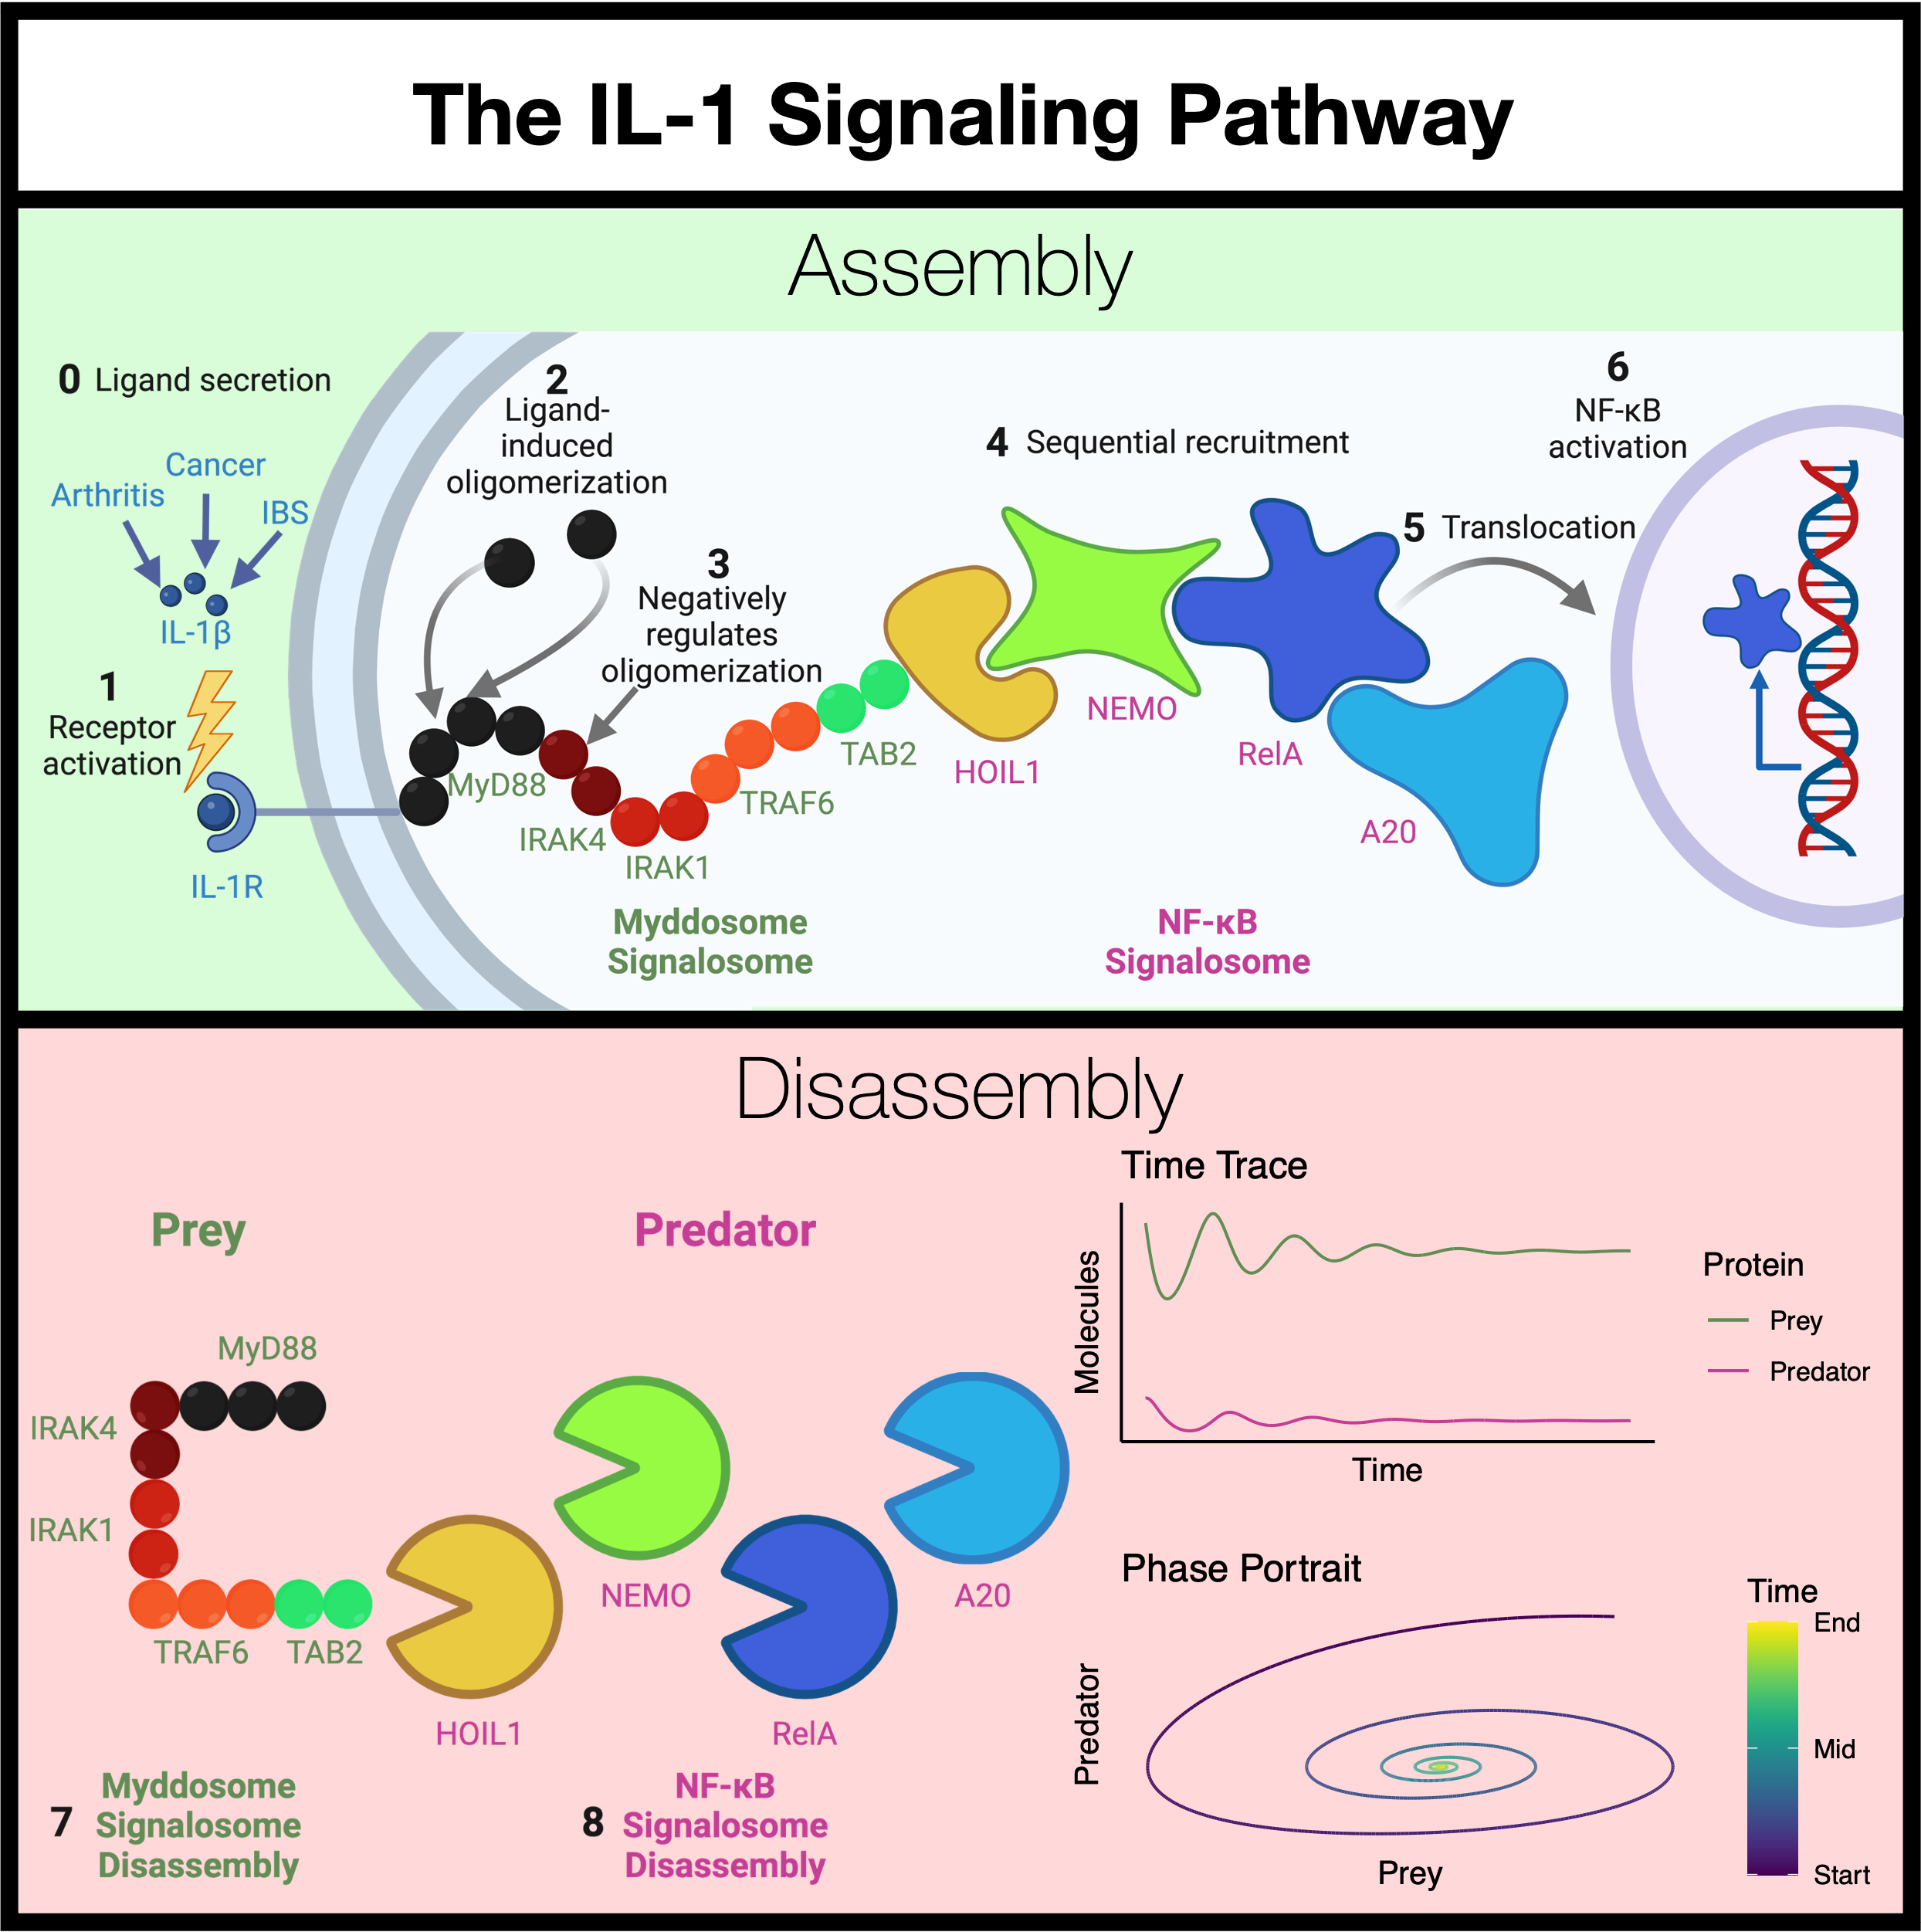
\includegraphics[width=0.8\textwidth, height=0.8\textheight, keepaspectratio]{img/Graphical_Abstract.png}}
\captionsetup{parbox=none}
\captionof{figure}[Graphical abstract]{\textbf{Graphical abstract.} (Designed using BioRender.com)}
\label{img:Graphical_Abstract}
\end{centering}

\section{Highlights}
\begin{itemize}
\item Two new membraneless organelles discovered using physics tools
\item IL-1 pathway proteins have ligand-induced sequential assembly
\item IRAK4 regulates MyD88 oligomer length
\item IL-1 pathway disassembly mechanism identified
\item Novel equations recapitulate IL-1 pathway dynamics
\item New image analysis pipeline tracks single-molecule changes
\end{itemize}

\cleardoublepage
\phantomsection
\addcontentsline{toc}{chapter}{Contents}
\tableofcontents
\chaptermark{Contents}

\cleardoublepage
\phantomsection
\addcontentsline{toc}{chapter}{\listfigurename}
\listoffigures
\chaptermark{List of Figures}

\cleardoublepage
\phantomsection
\addcontentsline{toc}{chapter}{List of Publications}
\chapter*{List of Publications}
\chaptermark{List of Publications}
\section*{Peer-reviewed}
\sectionmark{}

\begin{hangparas}{.5in}{1}
\setlength{\parskip}{0pt}
Cao F, \textbf{Deliz-Aguirre R}, Gerpott FH, Ziska E, Taylor MJ. Myddosome clustering in IL-1 receptor signaling regulates the formation of an NF-κB activating signalosome. EMBO Reports, e57233.

\textbf{Deliz-Aguirre R}, Cao F, Gerpott FH, Auevechanichkul N, Chupanova M, Mun Y, Ziska E, Taylor MJ. MyD88 oligomer size functions as a physical threshold to trigger IL1R Myddosome signaling. Journal of Cell Biology. 2021 May 6;220(7):e202012071.
\end{hangparas}

\section*{Pre-prints}
\begin{hangparas}{.5in}{1}
\setlength{\parskip}{0pt}
Srikanth N, \textbf{Deliz-Aguirre R}, Gola DK, Bilay M, Ziska E, Taylor MJ. IRAK4 autophosphorylation controls inflammatory signaling by activating IRAK oligomerization. bioRxiv. 2023:2023-12.

Cao F, \textbf{Deliz-Aguirre R}, Gerpott FH, Ziska E, Taylor MJ. Myddosome clustering in IL-1 receptor signaling regulates the formation of an NF-kB activating signalosome. bioRxiv. 2023:2023-01.

\textbf{Deliz-Aguirre R}, Cao F, Gerpott FH, Auevechanichkul N, Chupanova M, Mun Y, Ziska E, Taylor MJ. On demand MyD88 oligomerization is controlled by IRAK4 during Myddosome signaling. BioRxiv. 2020 Sep 3:2020-09.
\end{hangparas}

\cleardoublepage
\phantomsection
\chapter*{Abstract}
\addcontentsline{toc}{chapter}{Abstract}
\chaptermark{Abstract}
\sectionmark{}
Modularity is a recurring theme in biological networks where independent elements repeat and shuffle to produce novel functions. In innate immunity, supramolecular organizing centers (SMOCs) are an example of modularity, characterized by ligand-induced complex self-assembly, and signaling components increase in local concentration. The Myddosome is a SMOC that assembles in response to the ligand IL-1, a vital proinflammatory cytokine. The Myddosome-mediated IL-1 signaling pathway has been extensively characterized using biochemical methods, yet dynamic information remains limited. There are conflicting reports of how the IL-1 pathway proteins assemble, and it is unknown whether IL-1 pathway complexes disassemble. This thesis investigated the Myddosome-mediated IL-1 signal transduction dynamics, combining a completely new high-throughput image analysis pipeline, phase portrait analysis, a novel microscopy assay, and CRISPR/Cas9-edited live lymphoma cell lines.

Here, I show that the IL-1 pathway assembly has sequential steps, ligand-induced de novo oligomerization, proteins regulating oligomer size, and two modules: the Myddosome and NF-κB signalosomes. The upstream Myddosome signalosome (MyD88, IRAK4, IRAK1, TRAF6, TAB2) appears first, has no FRAP recovery, and shows positive internal feedback. The downstream NF-κB signalosome (HOIL1, NEMO, RelA, A20) appears later, recovers after FRAP, and negatively regulates the Myddosome signalosome. I also show, for the first time, that the IL-1 pathway disassembles after crossing a critical stoichiometric ratio, and that dynamical equations can recapitulate assembly-disassembly.

These results demonstrate how a SMOC-dependent pathway uses modularity to achieve regulation. Understanding signaling modules holds significant implications for elucidating the regulatory circuitry in biological networks. My high-throughput pipeline offers a promising approach to achieving this objective.
\vspace{1.0cm}
\\
keywords: \emph{IL-1 signaling, inflammation, protein dynamics, biophysics, systems biology}

\begin{center}
\selectlanguage{german}
{\Large Zusammenfassung}
\end{center}
\textit{Modularität ist ein wiederkehrendes Thema in biologischen Netzwerken, in denen sich unabhängige Elemente wiederholen und neu zusammensetzen, um neue Funktionen zu erzeugen. In der angeborenen Immunität sind supramolekular organisierende Zentren (SMOCs) ein Beispiel für Modularität, die durch eine ligandeninduzierte komplexe Selbstassemblierung gekennzeichnet sind und deren Signalkomponenten in ihrer lokalen Konzentration zunehmen. Das Myddosom ist ein SMOC, das sich als Reaktion auf den Liganden IL-1, ein wichtiges proinflammatorisches Zytokin, zusammensetzt. Der Myddosom-vermittelte IL-1-Signalweg wurde mit biochemischen Methoden umfassend charakterisiert, doch Informationen zur Dynamik sind weiterhin begrenzt. Es gibt widersprüchliche Berichte darüber, wie die Proteine des IL-1-Signalwegs zusammengesetzt werden, und es ist nicht bekannt, ob die Komplexe des IL-1-Signalwegs wieder abgebaut werden. In dieser Arbeit wurde die Dynamik der Myddosom-vermittelten IL-1-Signaltransduktion untersucht, wobei eine völlig neue Hochdurchsatz-Bildanalyse-Pipeline, eine Phasenporträtanalyse, ein neuartiger Mikroskopie-Assay und CRISPR/Cas9-editierte lebende Lymphomzelllinien kombiniert wurden.}

\textit{Hier zeige ich, dass der Aufbau des IL-1-Signalwegs sequenzielle Schritte, eine ligandeninduzierte De-novo-\\Oligomerisierung, Proteine, die die Oligomergröße regulieren, und zwei Module umfasst: das Myddosom und die NF-κB-Signalosome. Das stromaufwärts gelegene Myddosom-Signalosom (MyD88, IRAK4, IRAK1, TRAF6, TAB2) erscheint zuerst, zeigt keine Erholung in FRAP-Experimenten und zeigt eine positive interne Rückkopplung. Das nachgeschaltete NF-κB-Signalosom (HOIL1, NEMO, RelA, A20) erscheint später, erholt sich nach FRAP und reguliert das Myddosom-Signalosom negativ. Ich zeige auch zum ersten Mal, dass sich der IL-1-Signalweg nach Überschreiten eines kritischen stöchiometrischen Verhältnisses auflöst und dass dynamische Gleichungen den Zusammenbau und den Abbau nachbilden können.}

\textit{Diese Ergebnisse zeigen, wie ein SMOC-abhängiger Signalweg Modularität zur Regulierung einsetzt. Das Verständnis von Signalisierungsmodulen ist von großer Bedeutung für die Aufklärung der regulatorischen Schaltkreise in biologischen Netzwerken. Meine Hochdurchsatz-Pipeline bietet einen vielversprechenden Ansatz, um dieses Ziel zu erreichen.}
\vspace{1.0cm}

\textit{Schlüsselwörter:} IL-1-Signalisierung, Entzündung, Protein-Dynamik, Biophysik, Systembiologie.
\selectlanguage{english}

\cleardoublepage
\phantomsection
\chapter*{Acknowledgements}
\addcontentsline{toc}{chapter}{Acknowledgements}
\epigraph{Alone we can do so little; together we can do so much.}{Hellen Keller}
\chaptermark{Acknowledgements}
\sectionmark{}
I am grateful to my mentor, Dr. Marcus J. Taylor, whose patience and supervision were instrumental in the success of this interesting project. Your attention to detail and pursuit of improvement made my doctoral studies an enriching experience. Your mentorship unlocked abilities within me I never dreamed were possible--it transformed my perspective on what I am capable of achieving. For this and more, thank you.

I am indebted to my Thesis Advisory Committee. Prof. Dr. Arturo Zychlinsky, your leadership style embodies the principle that true leadership is rooted in selfless dedication to helping others, igniting curiosity in all, and maintaining equity. Dr. Olivia Majer, your encouragement, positive attitude, and lessons on balance were indispensable to this learning journey. Thank you for your continuous help and feedback, especially with presentations and writing. I enjoyed hearing your innate immunity perspective, and vivid lab stories in our joint lab meetings. Prof. Dr. Simone Reber, your networking skills and “elegance in simplicity” approach to scientific communication set an example for me. I appreciate how you used the joint lab meetings to teach us how to think quantitatively---I will forever use medians. Prof. Dr. Elena Levashina, you have emphasized the bigger picture, and reminded me that science exists to enlighten and inspire others, an influence I will carry on.

I would like to thank everyone in the Taylor lab. Dr. Fakun Cao, your good temperament and honesty has been a blessing. I appreciate all you taught me, from microscopy to critical thinking. Niranjan A. Srikanth you are a superb listener who radiates calmness. Thanks for all the lessons in biophysics--and that anything can be done in R. Dr. Fenja Gerpott, my wise predecessor, your support, tips and encouragement to keep on has been invaluable. Elke Ziska, my desk neighbor for years, thanks for being enthusiastic and sharing research victories together. Nichanok “Nicha” Auevechanichkul, your happiness is infectious and brings much joy to all of us in the lab. I will forever remember the protocol songs. Mauriz Lichtenstein, your dry humor doubled as the voice of reason. Finn Lobnow, your support in all things technical showed you are as resourceful as you are caring. Paulina Dirvanskytė, your humor provided much-needed lightness in challenging times. Claudia Abad-Baucells, your prevailing spirit and determination taught me that challenges are to be overcome with unwavering resolve. Elba del Val, thank you for teaching me biology terms in Spanish, and for all the laughs we had fighting R. Kathrin Lättig, your creativity knows no limits, and you always made us smile. Anna Kulesza, your adventurous nature and musical sessions have made the journey more enjoyable. Mariam Chupanova, your Midas touch that turns everything into gold and endless knowledge has been truly awe-inspiring. Alex Schmidt, your unique perspective definitely made us all rethink what we know about biology. My sincerest gratitude to Viviane Finke, YeVin Mun, Hans Lindig, Dr. Florenz Cruz, and Margaux Bilay who have each contributed to this lab experience in their own way.

I am very grateful for the collaborators at the Max Planck Institute of Molecular Cell Biology and Genetics (Dresden, Germany) who made me feel like family. Prof. Dr. Stephan W. Grill, your infectious energy and unquenchable curiosity fueled an exciting learning environment. Welcoming me into your lab as one of your own has meant more than words can express. Prof. Dr. Arjun Narayanan, your unique perspective, especially through the physics lens, has transformed how I approach science. I appreciate all the patience you had in showing me the world of phase portraits and dynamical systems. Your rational, calm approach, coupled with the final push you provided, has been instrumental in the completion of this thesis. Words cannot express how deeply thankful I am for going above and beyond, providing dependable support. Dr. Victoria Yan, thanks for being a biology-physics interpreter, and for sharing the world of \emph{C. elegans}. Archit Bhatnagar, thanks for the discussions on how to conceptualize numbers and visualize them. It taught me a lot about data analysis. Jan Geisler, thanks for all the help in coding tools for understanding complex systems. I am very appreciative to everyone in the Grill Lab for welcoming me, and offering input on this work.

Thanks to the Majer Lab of the Max Planck Institute for Infection Biology (MPI-IB) for always brightening up my day, especially Harshita Mishra, Anna Dingfelder, Dennis Hinkel, Oliver Thieck, Dr. Ee Lyn Lim, Fenja Blank and Ioulia Sampani. My heartfelt thanks to the Reber lab (MPI-IB) for all the wonderful biophysics discussions. Dr. Abin Biswas, I appreciate all your research insider tips, and your lessons on statistics. I would also like to thank the Zychlinsky lab (MPI-IB) for their relentless encouragement. Dr. Garth L. Burn, I appreciate the expert advice you provided me, from how to become a better professional scientist to learning the literature and reviewing my writing. I am extremely grateful that you reviewed this thesis so thoroughly. Sergio González San Miguel, thank you for always making fascinating questions that I never thought about my research. I also appreciate all the hours you dedicated to reviewing this thesis. 

I would also like to thank our collaborators, particularly Prof. Dr. Kevin Thurley from the German Rheumatism Research Center “DRFZ” (Berlin, Germany), who also served as a member of my Thesis Advisory Committee, and to Jana Wolf and Fabian Konrath of the Max Delbrück Center for Molecular Medicine (Berlin, Germany), for their ideas on cell signaling.

I'm grateful to the MPI-IB Administration, including Dr. Franziska Streßmann, Sybille Kim, Veronika Majer, Sarah Kuck, Cornelia Heinz, and EDV for providing dependable support. Dr. Susann Beetz, thank you for inviting me to Berlin and making me feel part of the institute. Dr. Piet Jonas, thank you for all the clever ideas on coding and all things computational.

My appreciation extends to the Center of Infection Biology and Immunity (ZIBI) people for insightful discussions, especially Dr. Juliane Kofer for helping me settle into Berlin smoothly, and to Dr. Linn Lundvall for attentive listening and advice.

I would like to thank the Max Planck Society for funding my doctoral fellowship. I would also like to acknowledge the Max Planck Computing and Data Facility (MPCDF) for allowing me to perform computations on the high-performance computing (HPC) system Raven, Cobra and Draco, and for providing technical support.

I would like to thank the doctoral defense commission, Prof. Dr. Ana Pombo, Prof. Dr. Andrew Plested, Prof. Dr. Arjun Narayanan, Prof. Dr. Chiara Romagnani and Prof. Dr. Thomas Sommer. Not only did each of you selflessly volunteer to come to my defense, but the kindness in our interactions is moving. Prof. Dr. Chiara Romagnani, I would also like to thank you for your career advice, and as a former ZIBI student representative, thank you for being a wonderful and diplomatic ZIBI faculty spokesperson. Us, students, felt included and listened.

I am very grateful to all my previous mentors who gave me the skills to succeed professionally, and encouraged me to become a scientist. I am especially grateful to Dr. Sebastian R. Schmidl for making me discover my true passion in his lab, for encouraging me to further my training in Germany, and for offering his support and guidance throughout the years.

Last but not least, my deepest gratitude goes out to my beloved partner, family, and friends, who always lend an ear when needed, reminding me to think forward, and of the power of love and perseverance. Your faith in me has been my strength, and your love, my sustenance. To those back home, I appreciate all the sacrifices you made, and your encouragement to chase my dreams in Germany. This achievement is as much yours as it is mine.

Thank you, all, from the bottom of my heart!

\chapter*{Contributor Roles Taxonomy Author Statement}
\chaptermark{CRediT Author Statement}
The thesis manuscript prepared by Rafael Deliz-Aguirre benefited greatly from the contributions of Marcus J. Taylor, Arjun Narayanan, Arturo Zychlinsky, Fakun Cao, Garth L. Burn, Olivia Majer, Simone Reber, Sergio Gonzalez San Miguel, Niranjan A. Srikanth, Paulina Dirvanskytė, and Finn Lobnow who provided extensive reading, insightful comments, and constructive feedback.

Figure panel contributions are listed in each figure legend. Results contributions are listed below.\footnote{Style from Contributor Roles Taxonomy (CRediT) Author Statement: Allen, L. O’Connell, A. \& Kiermer, V. (2019). How can we ensure visibility and diversity in research contributions? How the Contributor Role Taxonomy (CRediT) is helping the shift from authorship to contributorship. Learned Publishing.}

\section*{Chapter~\ref{chapter:p1}}
\begin{itemize}
\item \textbf{Rafael Deliz-Aguirre}: Methodology, Software, Validation, Formal Analysis, Investigation, Data Curation, Writing - Original Draft, Writing - Review \& Editing, Visualization.

\item \textbf{Fakun Cao}: Methodology, Validation, Formal Analysis, Investigation, Data Curation, Writing - Original Draft, Writing - Review \& Editing, Visualization.

\item \textbf{Elke Ziska}: Methodology, Validation, Investigation, Writing - Review \& Editing.

\item \textbf{Fenja H.U. Gerpott, Nichanok Auevechanichkul, Mariam Chupanoval}: Validation, Investigation, Writing - Review \& Editing.

\item \textbf{YeVin Mun}: Investigation, Writing - Review \& Editing.

\item \textbf{Alexander Shmidt}: Methodology, Software.

\item \textbf{Viviane Fenk}: Investigation, Data Curation.

\item \textbf{Marcus J. Taylor}: Conceptualization, Methodology, Validation, Formal Analysis, Investigation, Resources, Data Curation, Writing - Original Draft, Writing - Review \& Editing, Visualization, Supervision, Project Administration, Funding Acquisition.

\end{itemize}

\section*{Chapter~\ref{chapter:p2}}
\begin{itemize}

\item \textbf{Rafael Deliz-Aguirre}: Conceptualization, Methodology, Software, Validation, Formal Analysis, Investigation, Data Curation, Visualization, Writing - Original Draft, Writing - Review \& Editing.

\item \textbf{Fakun Cao}: Validation, Formal Analysis, Investigation, Data Curation, Writing - Review \& Editing, Visualization.

\item \textbf{Niranjan A. Srikanth}: Investigation, Validation, Writing - Review \& Editing.

\item \textbf{Elke Ziska, Claudia Abad-Baucells, Elba del Val}: Investigation, Validation.

\item \textbf{Kathrin Lättig, Anna Kulesza}: Validation.

\item \textbf{Arjun Narayanan}: Conceptualization, Methodology, Writing - Review \& Editing, Supervision.

\item \textbf{Stefan W. Grill}: Methodology, Resources, Supervision, Project Administration.

\item \textbf{Marcus J. Taylor}: Conceptualization, Methodology, Investigation, Resources, Writing - Review \& Editing, Supervision, Project Administration, Visualization.

\end{itemize}

\cleardoublepage
\phantomsection
\chapter*{List of Abbreviations}
\addcontentsline{toc}{chapter}{List of Abbreviations}
\chaptermark{List of Abbreviations}
% It is on a separate document
\makeatletter
\chaptermark{List of Abbreviations}
\sectionmark{}
% \newcommand{\tocfill}{\cleaders\hbox{$\m@th \mkern\@dotsep mu . \mkern\@dotsep mu$}\hfill} % leading dots
\newcommand{\tocfill}{\cleaders\hbox{}\hfill}
\makeatother
\newcommand{\abbrlabel}[1]{\makebox[3cm][l]{\textbf{#1}\ \tocfill}}
\newenvironment{abbreviations}{\begin{list}{}{\renewcommand{\makelabel}{\abbrlabel}%
        \setlength{\labelwidth}{3cm}\setlength{\leftmargin}{\labelwidth+\labelsep}%
                                              \setlength{\itemsep}{0pt}}}{\end{list}}
                     
\begin{spacing}{0.75}
\begin{abbreviations}
% Paste abbreviations below   
\item[ABIN] A20-Binding Inhibitor of NF-κB
\item[AI] Artificial Intelligence
\item[ALS] Amyotrophic Lateral Sclerosis
\item[CAPS] Cryopyrin-Associated Periodic Syndrome
\item[CARD] Caspase Recruitment Domain
\item[CCD] Charge-Coupled Device
\item[CD] Cluster of Differentiation
\item[CI] Confidence Interval
\item[CMOS] Complementary Metal-Oxide-Semiconductor
\item[COVID-19] Coronavirus Disease 2019
\item[CPU] Central Processing Unit
\item[CRediT] Contributor Roles Taxonomy
\item[CRISPR] Clustered Regularly Interspaced Short Palindromic Repeats
\item[cryoEM] Cryo-Electron Microscopy
\item[CSV] Comma-Separated Values
\item[Ct] Cycle of Threshold
\item[DAPI] 4′, 6-Diamidino-2-Phenylindole
\item[DD] Death Domain
\item[DISC] Death-Inducing Signaling Complex
\item[DMSO] Dimethyl Sulfoxide
\item[DNA] Deoxyribonucleic Acid
\item[e.g.] Exempli Gratia (\emph{for example}, Latin)
\item[EDV] Elektronische Datenverarbeitung
\item[eGFP] Enhanced Green Fluorescent Protein
\item[EL4] Murine T-lymphoma Cell Line
\item[EL4.NOB-1] EL4 Cell Line with No Binding-1
\item[ELISA] Enzyme-Linked Immunosorbent Assay
\item[ERK] Extracellular-Signal Regulated Kinase
\item[FAS] Fatty Acid Synthase
\item[FIJI] Fiji Is Just ImageJ
\item[FRAP] Fluorescence Recovery After Photobleaching
\item[GB] Gigabyte
\item[GFP] Green Fluorescent Protein
\item[GHz] Gigahertz
\item[GPU] Graphics Processing Unit
\item[HeLa] Henrietta Lacks (Cell Line)
\item[HOIL1] Heme-Oxidized Iron Regulatory Protein 2 Ubiquitin Ligase 1
\item[HP] High Performance
\item[HPC] High-Performance Computing
\item[HU] Humboldt University of Berlin
\item[i.e.] id est (\emph{that is}, Latin)
\item[ID] Identifier
\item[IFS] Immuno-Fluorescence Staining
\item[IKK] IκB Kinase
\item[IL-1] Interleukin-1
\item[IL-1R] IL-1 Receptor
\item[IL-2] Interleukin-2
\item[IL] Interleukin
\item[ImageJ] Image Processing and Analysis in Java
\item[IP] Immunoprecipitation
\item[IRAK] IL-1R Associated Kinase
\item[IRAK1] Interleukin-1 Receptor-Associated Kinase 1
\item[IRAK2] Interleukin-1 Receptor-Associated Kinase 2
\item[IRAK4] Interleukin-1 Receptor-Associated Kinase 4
\item[IRF] Interferon Regulatory Factor
\item[IRP2] Iron-Responsive Element-Binding Protein 2
\item[IκB] Inhibitor κ B
\item[JCB] Journal of Cell Biology
\item[JNK] c-Jun N-terminal kinase
\item[K63-Ub] Lysine 63-Linked Ubiquitin Chain
\item[KO] Knockout
\item[LAP] Linear Assignment Problem
\item[LC] Liquid Chromatography
\item[LoG] Laplacian of Gaussian
\item[LPS] Lipopolysaccharide
\item[LUBAC] Linear Ubiquitin Chain Assembly Complex
\item[LUT] Look-Up Table
\item[M1-Ub] Methionine 1-Linked Ubiquitin Chain
\item[MAD] Median Absolute Deviation
\item[MAP] Mitogen-Activated Protein
\item[MAPK] Mitogen-Activated Protein Kinase
\item[MATLAB] MATrix LABoratory
\item[MAVS] Mitochondrial Antiviral Signaling Protein
\item[metR] Methionine Repressor
\item[MPCDF] Max Planck Computing and Data Facility
\item[MPI-IB] Max Planck Institute for Infection Biology
\item[MS] Mass Spectrometry
\item[mScarlet] Modified Red Fluorescent Protein
\item[MyD88] Myeloid Differentiation Primary Response 88
\item[ND2] Nikon Imaging Software (NIS)-Elements Document Version 2
\item[NEMO] NF-κB Essential Modulator
\item[NF-κB] Nuclear Factor κ-Light-Chain-Enhancer of Activated B-cells
\item[OpenCV] Open Source Computer Vision Library
\item[OS] Operating System
\item[P-Values] Probability Values
\item[PALM] Photoactivated Localization Microscopy
\item[PAMP] Pathogen-Associated Molecular Pattern
\item[PARLEYS] Phase Portrait Analysis and Relative Kinetics Comparison Localization Analysis with Extraction of Data Yielding Statistics
\item[PCA] Principal Component Analysis
\item[PCR] Polymerase Chain Reaction
\item[PIRATES] Pipeline for Image Analysis with Reference Images, Automated Tracking, Extraction of Intensities, and Segmentation
\item[PP] Phase Portrait
\item[PPAR] Peroxisome Proliferation Activator Receptor
\item[PPI] Protein-Protein Interaction
\item[PRR] Pattern Recognition Receptor
\item[RA] Rheumatoid Arthritis
\item[RAM] Random Access Memory
\item[RANK] Receptor Activator of NF-κB
\item[RAR] Retinoic Acid Receptor
\item[RAS] Rat Sarcoma
\item[RelA] NF-κB Subunit
\item[rev] Reverse
\item[RH] Ras Homolog
\item[RING] Really Interesting New Gene
\item[RLR] RIG-I-Like Receptor
\item[RNA] Ribonucleic Acid
\item[ROI] Region of Interest
\item[sCMOS] Scientific Complementary Metal-Oxide-Semiconductor
\item[SD] Standard Deviation
\item[SEM] Standard Error of the Mean/Median
\item[SH2] Src Homology 2
\item[SIM] Structured Illumination Microscopy
\item[SLB] Supported Lipid Bilayer
\item[SMOC] Supramolecular Organizing Center
\item[SNR] Signal-to-Noise Ratio
\item[SRC] Proto-Oncogene Tyrosine-Protein Kinase Src
\item[STORM] Stochastic Optical Reconstruction Microscopy
\item[TAB] TGF-β-Activated Kinase 1 (TAK1)-Binding Protein
\item[TAB2] TAB 2
\item[TAK1] TGF-β-Activated Kinase 1
\item[TIFF] Tagged Image File Format
\item[TIR] Toll/Interleukin-1 Receptor
\item[TIRAP] Toll/Interleukin-1 Receptor Domain-Containing Adaptor Protein
\item[TIRF] Total Internal Reflection Fluorescence
\item[TIRF-M] TIRF Microscopy
\item[TLR] Toll-Like Receptor
\item[TLR4] Toll-Like Receptor 4
\item[TNF] Tumor Necrosis Factor
\item[TRADD] TNF Receptor Superfamily Member 1A-Associated Via Death Domain
\item[TRAF] TNF Receptor-Associated Factor
\item[TRAF6] TNF Receptor-Associated Factor 6
\item[TRIF] TIR Domain-Containing Adaptor Protein Inducing Interferon-β
\item[WT] Wild-Type
\item[XML] eXtensible Markup Language
\item[YYYYMMDD] Year Month Day

\begin{comment}
\item[ABIN] A20-Binding Inhibitor of NF-κB
\item[ACN] Acetonitrile
\item[AHA] Azidohomoalanine
\item[AHD] ABIN Homology Domain
\item[AI] Artificial Intelligence
\item[ALS] Amyotrophic Lateral Sclerosis
\item[AP-1] Activator Protein 1
\item[ATP] Adenosintriphosphate
\item[BMDC] Bone Marrow-Derived Dendritic Cell
\item[BMDM] Bone Marrow-Derived Macrophage
\item[bp] Base Pair
\item[BRCA1] Breast Cancer Gene 1
\item[BSA] Bovine Serum Albumin
\item[c-Jun] Cellular Jun Proto-Oncogene
\item[CAA] Chloroacetamide
\item[CAPS] Cryopyrin-Associated Periodic Syndrome
\item[CARD] Caspase Recruitment Domain
\item[CCD] Charge-Coupled Device
\item[CD] Cluster of Differentiation
\item[CD40] Cluster of Differentiation 40
\item[CHX] Cycloheximide
\item[CI] Confidence Interval
\item[CMOS] Complementary Metal-Oxide-Semiconductor
\item[COVID-19] Coronavirus Disease 2019
\item[CPU] Central Processing Unit
\item[CRediT] Contributor Roles Taxonomy
\item[CRISPR] Clustered Regularly Interspaced Short Palindromic Repeats
\item[cryoEM] Cryo-Electron Microscopy
\item[CSV] Comma-Separated Values
\item[Ct] Cycle of Threshold
\item[CYLD] Ubiquitin Carboxyl-Terminal Hydrolase Cylindromatosis
\item[DAMP] Danger Associated Molecular Pattern
\item[DAPI] 4′, 6-Diamidino-2-Phenylindole
\item[DD] Death Domain
\item[dH\textsubscript{2}O] Distilled Water
\item[DISC] Death-Inducing Signaling Complex
\item[DLBCL] Diffuse Large B-cell Lymphoma
\item[DMSO] Dimethyl Sulfoxide
\item[DNA] Deoxyribonucleic Acid
\item[DTT] Dithiothreitol
\item[DUB] Deubiquitinating Enzyme
\item[e.g.] Exempli Gratia (\emph{for example}, Latin)
\item[EDTA] Ethylenediaminetetraacetic Acid
\item[EDV] Elektronische Datenverarbeitung
\item[eGFP] Enhanced Green Fluorescent Protein
\item[EGFR] Epidermal Growth Factor Receptor
\item[EL4] Murine T-lymphoma Cell Line
\item[EL4.NOB-1] EL4 Cell Line with No Binding-1
\item[ELISA] Enzyme-Linked Immunosorbent Assay
\item[ERK] Extracellular-Signal Regulated Kinase
\item[EtOH] Ethanol
\item[FACS] Fluorescence Activated Cell Sorting
\item[FAS] Fatty Acid Synthase
\item[FBS] Fetal Bovine Serum
\item[FIJI] Fiji Is Just ImageJ
\item[FRAP] Fluorescence Recovery After Photobleaching
\item[fwd] Forward
\item[GB] Gigabyte
\item[GFP] Green Fluorescent Protein
\item[GHz] Gigahertz
\item[GPCR] G Protein-Coupled Receptor
\item[GPU] Graphics Processing Unit
\item[gRNA] Guide RNA
\item[GSDMD] Gasdermin
\item[HEK] Human Embryonic Kidney
\item[HEK293] Human Embryonic Kidney 293 (Cell Line)
\item[HeLa] Henrietta Lacks (Cell Line)
\item[HIV] Human Immunodeficiency Virus
\item[HLA-B27] Human Leukocyte Antigen B27
\item[HOIL1] HOIL-1-Interacting Protein
\item[HOIP] HOIL-1-Interacting Protein
\item[HP] High Performance
\item[HPC] High-Performance Computing
\item[HRP] Horse Radish Peroxidase
\item[HU] Humboldt University of Berlin
\item[i.e.] id est (\emph{that is}, Latin)
\item[ID] Identifier
\item[IFN] Interferon
\item[IFS] Immuno-Fluorescence Staining
\item[IKK] IκB Kinase
\item[IKK1] Inhibitor of NF-κB Kinase Subunit α
\item[IKK2] Inhibitor of NF-κB Kinase Subunit β
\item[IKKg] Inhibitor of NF-κB Kinase Subunit γ
\item[IL-1] Interleukin-1
\item[IL-10] Interleukin-10
\item[IL-12] Interleukin-12
\item[IL-18] Interleukin-18
\item[IL-18R] Interleukin-18 Receptor
\item[IL-1R] IL-1 Receptor
\item[IL-1R1] Interleukin-1 Receptor 1
\item[IL-1R2] Interleukin-1 Receptor 2
\item[IL-1R3] Interleukin-1 Receptor 3
\item[IL-1Ra] Interleukin-1 Receptor Antagonist
\item[IL-1RAcP] IL-1R Accessory Protein
\item[IL-1RN] Interleukin-1 Receptor Antagonist
\item[IL-2] Interleukin-2
\item[IL-6] Interleukin-6
\item[IL] Interleukin
\item[ImageJ] Image Processing and Analysis in Java
\item[IP] Immunoprecipitation
\item[IRAK] IL-1R Associated Kinase
\item[IRAK1] Interleukin-1 Receptor-Associated Kinase 1
\item[IRAK2] Interleukin-1 Receptor-Associated Kinase 2
\item[IRAK4] Interleukin-1 Receptor-Associated Kinase 4
\item[IRF5] Interferon Regulatory Factor 5
\item[IRF] Interferon Regulatory Factor
\item[IRP2] Iron-Responsive Element-Binding Protein 2
\item[IκB] Inhibitor κ B
\item[JCB] Journal of Cell Biology
\item[JNK] c-Jun N-terminal kinase
\item[K11-Ub] Lysine 11-Linked Ubiquitin Chain
\item[K48-Ub] Lysine 48-Linked Ubiquitin Chain
\item[K63-Ub] Lysine 63-Linked Ubiquitin Chain
\item[kDa] Kilodalton
\item[KO] Knockout
\item[LAP] Linear Assignment Problem
\item[LC] Liquid Chromatography
\item[LLPS] Liquid-Liquid Phase Separation
\item[LoG] Laplacian of Gaussian
\item[LPS] Lipopolysaccharide
\item[LUBAC] Linear Ubiquitin Chain Assembly Complex
\item[LUT] Look-Up Table
\item[M1-pUb] Methionine 1-Linked polyUbiquitin Chain
\item[M1-Ub] Methionine 1-Linked Ubiquitin Chain
\item[mAB] Monoclonal Antibody
\item[MAD] Median Absolute Deviation
\item[MAP] Mitogen-Activated Protein
\item[MAPK] Mitogen-Activated Protein Kinase
\item[MAPKKK] MAP Kinase Kinase Kinase
\item[MATLAB] MATrix LABoratory
\item[MAVS] Mitochondrial Antiviral Signaling Protein
\item[MEF] Mouse Embryonic Fibroblast
\item[metR] Methionine Repressor
\item[MKK] MAP Kinase Kinase
\item[MPCDF] Max Planck Computing and Data Facility
\item[MPI-IB] Max Planck Institute for Infection Biology
\item[mRNA] Messenger RNA
\item[MS] Mass Spectrometry
\item[mScarlet] Modified Red Fluorescent Protein
\item[mTOR] Mammalian Target of Rapamycin
\item[MyD88] Myeloid Differentiation Primary Response 88
\item[NBD] NEMO Binding Domain
\item[ND2] Nikon Imaging Software (NIS)-Elements Document Version 2
\item[NEMO] NF-κB Essential Modulator
\item[NF-κB] Nuclear Factor κ-Light-Chain-Enhancer of Activated B-cells
\item[NLRP3] Leucine Rich Repeat-Containing Protein 2
\item[NZF] Npl4 Zinc Finger
\item[OpenCV] Open Source Computer Vision Library
\item[OS] Operating System
\item[p-IRAK1] Phosphorylated Interleukin-1 Receptor-Associated Kinase 1
\item[p-IRAK4] Phosphorylated Interleukin-1 Receptor-Associated Kinase 4
\item[P-Values] Probability Values
\item[PALM] Photoactivated Localization Microscopy
\item[PAMP] Pathogen-Associated Molecular Pattern
\item[PARLEYS] Phase Portrait Analysis and Relative Kinetics Comparison Localization Analysis with Extraction of Data Yielding Statistics
\item[PBMC] Peripheral Blood Mononuclear Cell
\item[PBS] Phosphate-Buffered Saline
\item[PCA] Principal Component Analysis
\item[PCR] Polymerase Chain Reaction
\item[PFA] Paraformaldehyde
\item[PI3K] Phosphoinositide-3-Kinase
\item[PIP2] Phosphatidylinositol 4,5-Bisphosphate
\item[PIRATES] Pipeline for Image Analysis with Reference Images, Automated Tracking, Extraction of Intensities, and Segmentation
\item[PMSF] Phenylmethylsulfonyl Fluoride
\item[PP] Phase Portrait
\item[PPAR] Peroxisome Proliferation Activator Receptor
\item[PPI] Protein-Protein Interaction
\item[PRR] Pattern Recognition Receptor
\item[pSILAC] Pulsed Stable Isotope Labeling by Amino Acids in the Culture
\item[RA] Rheumatoid Arthritis
\item[RAM] Random Access Memory
\item[RANK] Receptor Activator of NF-κB
\item[RAR] Retinoic Acid Receptor
\item[RAS] Rat Sarcoma
\item[RelA] NF-κB Subunit
\item[RelB] NF-κB Subunit RelB
\item[rev] Reverse
\item[RH] Ras Homolog
\item[RING] Really Interesting New Gene

\item[RIP1] Receptor-Interacting Protein 1
\item[RIP1-A20] Receptor-Interacting Protein 1 and A20
\item[RIPK1] Receptor-Interacting Serine-Kinase 1
\item[RLR] RIG-I-Like Receptor
\item[RNA] Ribonucleic Acid
\item[ROI] Region of Interest
\item[sCMOS] Scientific Complementary Metal-Oxide-Semiconductor
\item[SD] Standard Deviation
\item[SDS] Sodium Dodecyl Sulfate
\item[SDS-PAGE] SDS-Polyacrylamide Gel Electrophoresis
\item[SEM] Standard Error of the Mean/Median
\item[SH2] Src Homology 2
\item[SH3] Src Homology 3
\item[SHARPIN] SHANK-Associated RH Domain-Interacting Protein
\item[SIM] Structured Illumination Microscopy
\item[SLB] Supported Lipid Bilayer
\item[SMOC] Supramolecular Organizing Center
\item[SNP] Single Nucleotide Polymorphism
\item[SNR] Signal-to-Noise Ratio
\item[SRC] Proto-Oncogene Tyrosine-Protein Kinase Src
\item[ssODN] Single Stranded Oligodeoxynucleotides
\item[STORM] Stochastic Optical Reconstruction Microscopy
\item[TAB] TAK Binding Protein
\item[TAB2] TGF-β-Activated Kinase 1 (TAK1)-Binding Protein 2
\item[TAB3] TGF-β-Activated Kinase 1 (TAK1)-Binding Protein 3
\item[TAB] TGF-β-Activated Kinase 1 (TAK1)-Binding Protein
\item[TAK] TGFβ Activated Kinase
\item[TAK1] TGF-β-Activated Kinase 1
\item[TAK1-TAB] TGF-β-Activated Kinase 1 (TAK1)-Binding Protein
\item[Tax1bp1] Tax-1 Binding Protein 1
\item[TBS] Tris-Buffered Saline
\item[TFA] Trifluoroacetic Acid
\item[TGF-β] Transforming Growth Factor β
\item[TIFF] Tagged Image File Format
\item[TIR] Toll/Interleukin-1 Receptor
\item[TIRAP] Toll/Interleukin-1 Receptor Domain-Containing Adaptor Protein
\item[TIRF] Total Internal Reflection Fluorescence
\item[TIRF-M] Total Internal Reflection Fluorescence Microscopy
\item[TIRFM] Total Internal Reflection Fluorescence Microscopy
\item[TLR] Toll-Like Receptor
\item[TLR3] Toll-Like Receptor 3
\item[TLR4] Toll-Like Receptor 4
\item[TLR7] Toll-Like Receptor 7
\item[TLR] Toll-Like Receptor
\item[TNF] Tumor Necrosis Factor
\item[TNF-R] Tumor Necrosis Factor Receptor
\item[TNFAIP] TNFα Induced Protein
\item[TNFR] Tumor Necrosis Factor Receptor
\item[TNIK] Traf2- and Nck-Interacting Kinase
\item[TNIP] Tnfaip3 Interacting Protein
\item[TOLLIP] Toll-Interacting Protein
\item[TRADD] TNFRSF1A-Associated via Death Domain
\item[TRAF] TNF Receptor-Associated Factor
\item[TRAF6] TNF Receptor-Associated Factor 6
\item[TRAF7] TNF Receptor-Associated Factor 7
\item[TRAF] TNF Receptor-Associated Factor
\item[TRIF] TIR Domain-Containing Adaptor Protein Inducing Interferon-β
\item[UBAN] UBD in ABIN Proteins and NEMO
\item[UBD] Ubiquitin Binding Domain
\item[WT] Wild-Type
\item[XML] eXtensible Markup Language
\item[YYYYMMDD] Year Month Day
\end{comment}

\end{abbreviations}
\end{spacing}


\restoregeometry

\pagestyle{plain}

\mainmatter

\pagestyle{fancy}
\renewcommand{\headrulewidth}{0pt} % No header rule

% Even page headers (left-hand pages)
\fancyhead[LE]{\thepage\quad{\scshape\footnotesize\addfontfeatures{LetterSpace=18}\MakeTextLowercase{\leftmark}}}
\fancyhead[RE]{} % Nothing on the right

% Odd page headers (right-hand pages)
\fancyhead[LO]{} % Nothing on the left
\fancyhead[RO]{{\footnotesize {\rightmark}}\quad\thepage}


% Adjusting the footer of the plain page style for all chapter starting pages
\fancypagestyle{plain}{
    \fancyhf{}
    \renewcommand{\headrulewidth}{0pt}
    \renewcommand{\footrulewidth}{0pt}
    \fancyfoot[RO]{\makebox[\paperwidth][r]{\hspace*{\oddsidemargin}\thepage\hspace{\dimexpr\marginparwidth+1.75\marginparsep-0.25in\relax}}}
}

\mygeometry
\part{Introduction}
\restoregeometry
\chapter{What is Inflammation?}
\label{chapter:inflammation}
Homeostasis---the state of stability and health in multicellular organisms, is continually challenged by injury, infections, and tissue malfunction. Inflammation acts as a physiological response to these threats, working to restore homeostasis \autocite{Medzhitov_2008}. The balance of inflammation is crucial; both hypo- and hyper-inflammatory responses can be detrimental to health. Hypo-inflammation may result in a weakened immune response, leading to chronic infection \autocite{Tsirigotis_2016}, while a hyper-inflammatory response can give rise to autoimmunity and inflammatory disorders \autocite{Cavalli_2021}. How is inflammation activated and regulated to eliminate threats and maintain health? Addressing a subset of inflammatory processes is the central aim of this thesis.

\section{Inflammatory cascades}
\label{section:inflammation}
Inflammation plays a critical role in innate immune responses \autocite{Newton_2012} and can be triggered by various factors, such as microbes and injuries. As the first line of defense against threats, inflammation safeguards the organism \autocite{Diamond_2022}. The classical definition of inflammation, characterized by heat, redness, pain, swelling, and loss of function (Fig.~\ref{d:inflammation}), was established two millennia ago \autocite{Rather_1971}. Modern understanding recognizes that inflammatory pathways consist of four components: inducer/trigger, sensor, mediator, and effector \autocite{Medzhitov_2008}, all of which are composed of complex proteins and signaling molecules. Mediators in inflammatory signaling are specialized proteins that play a critical role in amplifying and transmitting signals during the inflammatory response. This thesis will describe the mediator cascade in specific proinflammatory responses. It will help clear whether signaling cascades transduce signals through preassembled complexes or ligand-induced oligomer assembly of complexes.


\begin{centering}
\centering{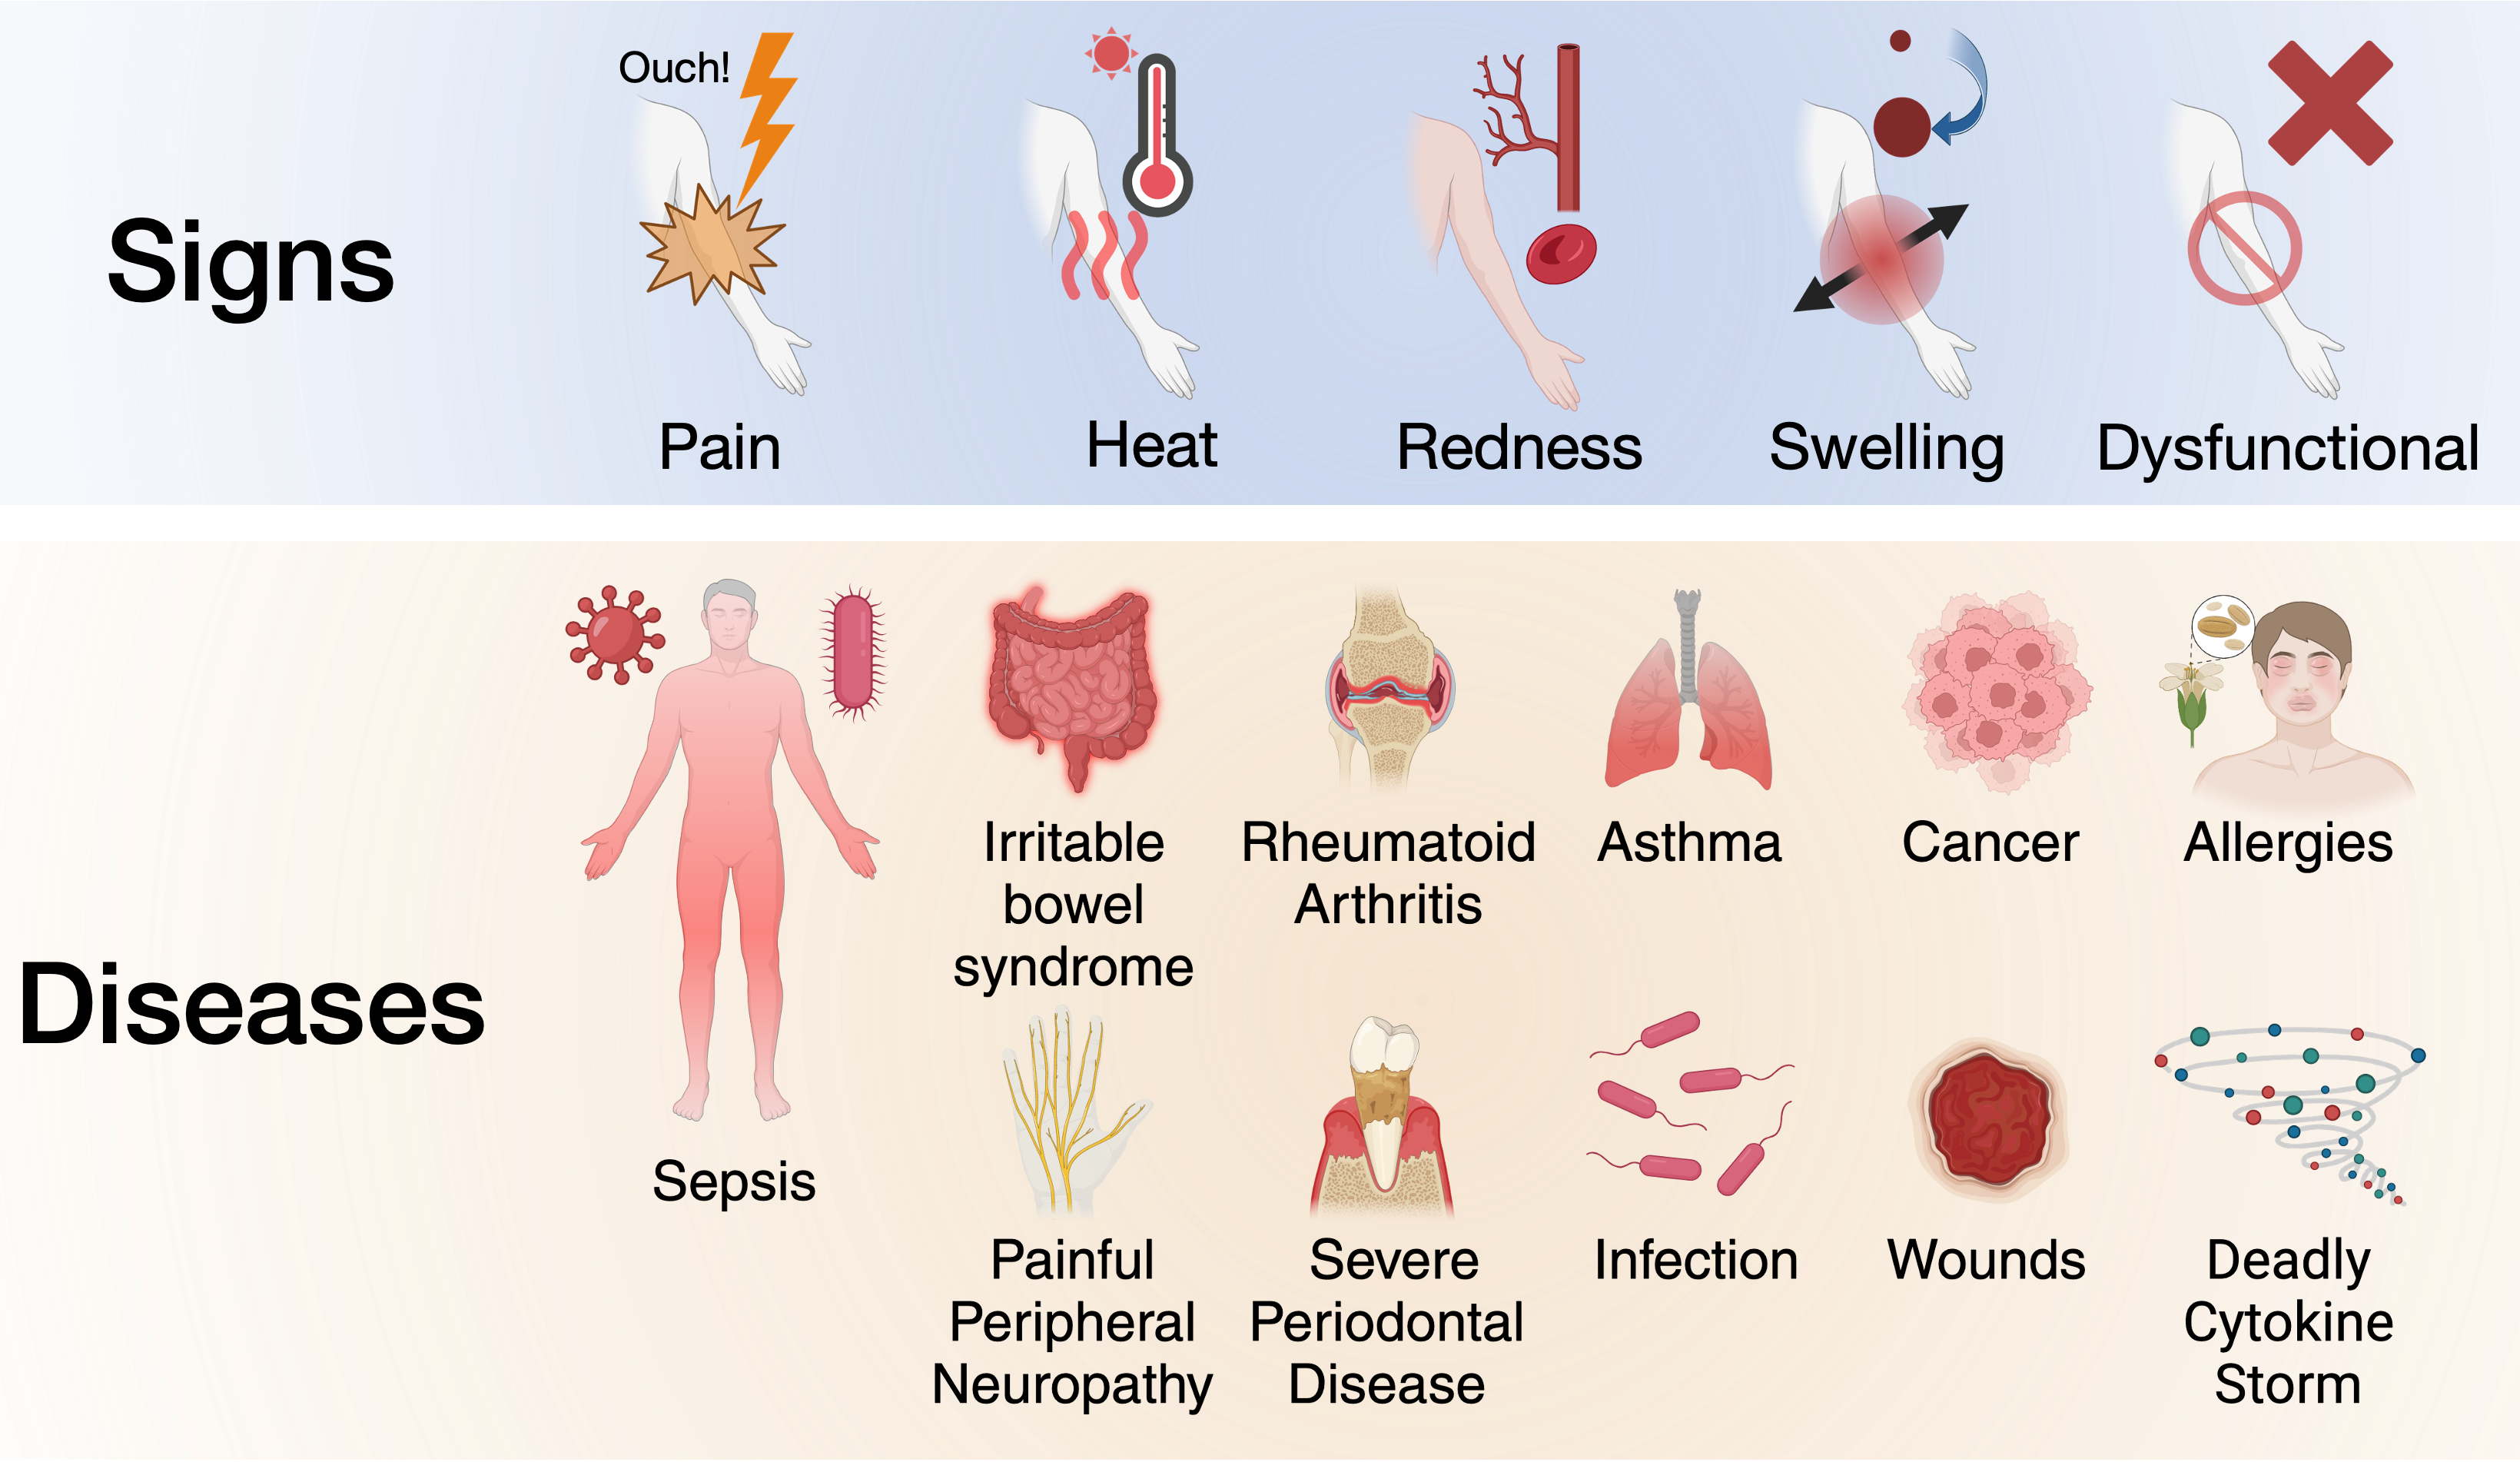
\includegraphics[width=\textwidth, height=\textheight, keepaspectratio]{img/inflammation.png}}
\captionsetup{parbox=none}
\captionof{figure}[Inflammatory responses are implicated in multiple diseases]{\textbf{Inflammatory responses are implicated in multiple diseases.} (Signs) The cardinal signs of inflammation are pain (\emph{dolor}), heat (\emph{calor}), redness (\emph{rubor}), swelling (\emph{tumor}) and loss of function (\emph{functio laesa}). (Diseases) Some of these pathologies can be triggered by microbes (sepsis and infection), autoimmune diseases (irritable bowel syndrome, rheumatoid arthritis), overactive immune systems (including allergies), cancer, neuropathy and asthma. Inflammation is also a normal response to wounds and severe periodontal disease. The similarities between wound response and cancer led to tumors to be called “wounds that do not heal \autocite{Dvorak_1986}.}
\label{d:inflammation}
\end{centering}
 
Interleukin-1{\textbeta} (IL-1{\textbeta}) is a well-known proinflammatory molecule that activates the IL-1 pathway \autocite{Dinarello_2019}. Dysregulation of this pathway, as seen in rheumatoid arthritis, or exposure to threats such as wounds can result in disease emergence, which has made the IL-1 pathway an appealing target for clinical research for which multiple therapies are available \autocite{Dinarello_2019}. Much of our current understanding of the IL-1 pathway overlaps with infection biology because of structural similarities between infection and specific inflammation receptors (specifically, TLR and IL-1, more on this later). Furthermore, both receptor families connect to the same downstream signaling pathways \autocite{Medzhitov_2008}\autocite{Dinarello_2009} \autocite{Takeuchi_2010}\autocite{ONeill_2009}\autocite{Fitzgerald_2020}. Because of this structural similarity, a lot of what is known about the mechanism of inflammatory receptors can be extrapolated from receptors that directly recognize microbes and viruses. Therefore, to understand biochemical and cell biological mechanism of inflammation, we have to also explore the receptors and signaling pathways cells use to detect and respond to microbes.
 
The innate immune system detects microbes by recognizing Pathogen-Associated Molecular Patterns (PAMPs), which are structural “signatures” unique to microbes \autocite{Akira_2003}. Examples of PAMPs include lipopolysaccharide (LPS), found in bacterial membranes, and the bacterial flagellum protein flagellin \autocite{Akira_2006}. A family of receptors called Pathogen Recognition Receptors (PRRs) directly bind and transduce signals in response to these microbial signatures. PRRs were hypothesized to exist before its proof \autocite{Janeway_1989}. The first discovered PPR was Toll-Like Receptor 1, identified in part due to its homology to the \emph{Drosophila} developmental protein, Toll \autocite{Anderson_1985}\autocite{Hashimoto_1988}. Yet, the link of Toll to infection was not immediately apparent; it was a gradual process.
 
In 1991, a seminal paper demonstrated that Toll and the Interleukin-1 Receptor (IL-1R) unexpectedly shares a cytoplasmic domain sequence now called the Toll/interleukin-1 receptor (TIR) domain \autocite{Sims_1988}\autocite{Gay_1991}. Subsequently, Toll was discovered to be an immune receptor responsible for antifungal responses in insects \autocite{Lemaitre_1996}. The first demonstrated PRR confirmed to be involved in infection was TLR4 in 1997 \autocite{Medzhitov_1997}. After, it was shown that these activate NF-κB, concretely tying infection and inflammatory responses \autocite{Alcamo_2001}. Nowadays, there are ten human known TLRs \autocite{ONeill_2013}, nine which have a TIR domain \autocite{ONeill_2013}. An activated TIR domain recruits an adaptor protein known as MyD88 \autocite{Muzio_1997}. Subsequently, TLR-activated MyD88 engages a downstream signaling pathways that is shared with the IL-1 pathway, and is the focus of this research. Given that TLR and IL-1 signaling are thought to be identical \autocite{Balka_2019}\autocite{Pereira_2023}, I will use known TLR/MyD88-dependent NF-κB signaling proteins to supplement the interrogation of the IL-1 pathway.
 
The primary objective of this research is to decipher the IL-1 inflammatory cascade with high spatial and temporal resolution. Because IL-1R and TLR share an intracellular domain, and signal through almost identical signaling pathways, this means that what we learn about IL-1R signaling can most likely be applied to TLR signal transduction. Therefore, this thesis will potentially discover universal mechanisms for how chemical signals initiate inflammation, enhancing our understanding of the innate immune system. In the future, these insights could aid the development of diagnostics and treatments for inflammatory diseases \autocite{Donath_2019}\autocite{Netea_2020}.
 
\chapter{The interleukin-1 signaling pathway}
\chaptermark{IL-1 pathway}
\label{chapter:pathway}
The IL-1 pathway is initiated when the proinflammatory cytokine IL-1{\textbeta} binds to the IL-1 Receptor (IL-1R) \autocite{Dinarello_2019}\autocite{Dinarello_2018}. This interaction culminates in NF-κB activation \autocite{Takeuchi_2002}. However, the intermediate steps in IL-1 signal transduction between receptor activation and nuclear translocation have not been completely identified. I will use light microscopy to resolve these intermediate steps.
 
IL-1 is an evolutionarily conserved cytokine found in most vertebrates, suggesting that it emerged early in vertebrate evolution \autocite{Bird_2002}\autocite{Rivers-Auty_2018}. Although most IL-1 family receptors (excluding IL-33R/IL1RL1) are evolutionarily related, their ligands exhibit greater evolutionary divergence \autocite{Rivers-Auty_2018}. However, despite the diversity of IL-1 family ligands, the common biochemical features suggest a unified signaling mechanism that is conserved across vertebrates. Because various vertebrates have similar IL-1 signaling machinery, this means mice cell lines are suitable for IL-1 experiments \autocite{Pinteaux_2020}.

\section{Supramolecular Organizing Centers}
\label{section:SMOC}
\sectionmark{SMOCs}
Within the field of innate immune signaling, a series of functionally similar large signaling oligomeric structures have been observed, termed supramolecular organizing centers (SMOCs) \autocite{Kagan_2014}. SMOCs are localized signaling complexes that amplify signals by increasing the local concentration of signaling components \autocite{Kagan_2014}. One hallmark of SMOCs includes the self-assembly of signaling proteins in receptors without intrinsic enzymatic activity \autocite{Kagan_2014}. Various signaling complexes have been designated as SMOCs, such as the Myddosome, the Fas ligand death-inducing signaling complex (FAS DISC), the PIDDosome, the RIG-I-like receptor (RLR) complex, and the Inflammasome (The concept of SMOCs is discussed in detail in \autocite{Kagan_2014}\autocite{Qiao_2015}\autocite{Tan_2019}.
 
A crucial SMOC question is if and how the individual components orchestrate self-assembly. The Myddosome could be used as a model of innate immune signaling.
 
\section{The Myddosome}
\subsection{Overview}
\label{section:intro_Myddosome}
The Myddosome is proposed to self-assemble in response to TLR and IL-1R activation, but this has not been quantified \autocite{Kagan_2014}\autocite{Lin_2010}\autocite{Latty_2018}. Analytical ultracentrifugation was employed to determine the MyD88:IRAK4 stoichiometry \autocite{Motshwene_2009}. Subsequently, the Myddosome crystal structure was solved in 2010, revealing a composition of 6\times MyD88, 4\times IRAK4, and 4\times IRAK2 molecules \autocite{Lin_2010}. Lin et al. hypothesized that the assembly mechanism involved self-oligomerization. However, the discrete steps involved in the formation of individual puncta have not been observed. A microscope-based approach would be needed to elucidate the individual assembly dynamics of individual complexes in live cells.
 
\subsection{The assembly dynamics are poorly characterized}
\subsectionmark{Assembly}
\label{subsection:assembly}
Almost a decade later after solving the crystal structure of Myddosomes, Latty et al. reported imaging fluorescently-labeled overexpressed MyD88 assembly using TIRF \autocite{Latty_2018}. This was the first attempt at resolving the dynamics of MyD88 in live cells \autocite{Latty_2018}. While Latty et al. found that MyD88 is LPS-inducible, and ligand strength correlated with NF-κB activation, intriguingly, they also found that Myddosomes coalesce to form “super-Myddosomes” \autocite{Latty_2018}. This result suggests that the spatial organization could play a vital role in regulating downstream signaling reactions. Indeed in 2009, their collaborators showed through ELISA that antibody-induced Toll-Like Receptor clustering enhances Myddosome-mediated signaling \autocite{Motshwene_2009}. Since then, we have shown through live cell microscopy that the spatial organization of Myddosomes is critical for signal transduction \autocite{Cao_2023}.
 
Yet, prior work on Myddosomes have had several limitations. (1) MyD88 overexpression leads to large aggregate formation in the cytosol in several cell lines \autocite{Jaunin_1998}\autocite{Nishiya_2007}. While the authors note their MyD88 structures were LPS-inducible \autocite{Latty_2018}\autocite{Moncrieffe_2020}, the assembly kinetics measured could be affected by overexpression artifacts. Since then, more precise genetic engineering tools have become increasingly accessible. Utilizing these latest innovations, we employed CRISPR/Cas9 to fluorescently label Myddosome proteins at endogenous loci, thereby preserving endogenous expression at physiological levels. While primary cell lines could offer an advantage, these have been limited to IRAK proteins \autocite{De_2018}. (2) When Latty et al. imaged MyD88, they had a dead time of around five minutes due to ligand administered prior to imaging. We addressed this concern of one of the reviewers by using SLB functionalized with IL-1 ligand. This allows us to image events prior to receptor activation. (3) Latty et al. also had low temporal resolution (one frame every 30 seconds), the formation of individual Myddosomes within a diffraction-limited spot remained unaddressed. To address this, we imaged at the faster frequency of one frame every 1-4 seconds.
 
How MyD88 oligomerizes to form a Myddosomes is unclear with conflicting reports. Analytical ultracentrifugation demonstrated that dimers might exist in solution \autocite{Moncrieffe_2020}. Also, certain forms of cancer have assembled Myddosomes in the cytosol in the absence of ligand \autocite{Ngo_2011}, possibly due to constitutively active MyD88 \autocite{Treon_2012}. On the flip side, crystallography suggested that Myddosomes are inducible self-assembling structures \autocite{Kagan_2014}\autocite{Lin_2010}. Yet, the aforementioned studies employ \emph{in vitro} endpoint strategies. They do not clarify if induced cells have preassembled Myddosomes or if they have ligand-induced oligomerization. Here, I will seek to determine which of these two models is correct, preformed scaffolds or ligand-induced \emph{de novo} oligomerization. I will use a microscopy-based approach that, unlike previous methodologies that analyze bulk cells, can resolve the dynamics of individual Myddosome complexes within a diffraction-limited spot. I will also use live cells which are closer to physiological conditions than the aforementioned \emph{in vitro} experiments. I adopted a highly quantitative image analysis approach which enabled me to compare diffraction-limited puncta with other methods, including solved crystal structures \autocite{Deliz-Aguirre_2021} (Chapter~\ref{chapter:p1}). My method has single-molecule resolution as fast as every second. This enables me to ascertain which model is correct---inducible self-assembly or preformed scaffolds. I hypothesize that not only is inducible self-assembly the correct model, but also that Myddosomes form as ligand-induced polymers. This task is important because it can give a basis for which SMOCs oligomerize to form signaling complexes.
 
The IL-1 Receptor-Associated Kinase (IRAK) family also plays a role in Myddosome assembly and signal transduction. However, their precise role in scaffold formation is still unclear. Immunoblotting revealed that the kinase activity of IRAK4 is not required for Myddosome assembly and NF-κB activation \autocite{DeNardo_2018}. Yet, endpoint assays cannot resolve individual assembly dynamics. To gain insights, my colleagues fluorescently labeled and imaged MyD88 alongside IRAK4 or IRAK1, and we knocked-out IRAK4 and IRAK1.
 
\subsection{Does the Myddosome disassemble? Multiple unreconciled views}
\subsectionmark{Disassembly}
\label{subsection:disassembly}
If Myddosome assembly drives signal transduction, it is likely that signal attenuation is controlled by the disassemble of the complex. However, the process of Myddosome disassembly remains poorly understood \autocite{Balka_2019}. Various models have been proposed to explain the TLR-signaling disassembly mechanism. For instance, in TLR2/4 signaling, Myddosomes are internalized post-stimulation via lipid rafts \autocite{Thieblemont_1998}\autocite{Thieblemont_1999}\autocite{Triantafilou_2004}\autocite{Triantafilou_2006}; \autocite{Kagan_2008}\autocite{Barbalat_2009}\autocite{Ruysschaert_2015}. However, it remains unclear whether the same mechanism applies to IL-1 signaling. Notably, TLR4 signaling, unlike IL-1 signaling, utilizes TIRAP/MAL as an adaptor protein to connect the receptor and MyD88 \autocite{Fitzgerald_2001}. Another model proposes that activated Myddosomes form vesicles, as observed in MyD88[L265P] cancers \autocite{Manček-Keber_2018}. Apart from internalization, activated Myddosomes could detach from the receptor and continue signaling, as assembled structures have been detected for hours after LPS stimulation \autocite{Balka_2019}\autocite{Nguyen_2017}. Therefore, an open question in the field is: how are Myddosomes disassembled to attenuate signaling?
 
\section{Downstream of the Myddosome}
\label{section:downstream}
The Myddosome serves as a molecular bridge between the receptor and its downstream signaling proteins. Several protein complexes are involved in the IL-1 pathway downstream of the Myddosome. A brief list of IL-1 pathway interactors is provided below. To understand how the Myddosome transduces its signal, we need to understand what downstream effector proteins it activates.
 
Tumor necrosis factor (TNF) receptor-associated factor 6 (TRAF6) is an adaptor protein with E3 ubiquitin ligase activity \autocite{Muzio_1997}\autocite{Cao_1996}\autocite{Naito_1999}. A solved crystal structure revealed that TRAF6 has three potential binding sites for IRAK1 \autocite{Ye_2002}. However, it is not known when these components interact. If IRAK1 and TRAF6 interact, then one can expect their assembly to be temporally close.
 
The TNF-Activated Kinase 1 (TAK1)-binding protein (TABs) TAK1-TABs complex interacts with the Mydddosome and is ubiquitinated by \\  TRAF6 \autocite{Deng_2000}\autocite{Wang_2001}\autocite{Kanayama_2004}\autocite{Wertz_2004}\autocite{Xia_2009}\autocite{Ajibade_2013}. However, this association is based on an immunoprecipitation experiment \autocite{Kanayama_2004}. As IRAK1 and TRAF6 are direct interactors \autocite{Ye_2002}, and TAB2 interacts with \\ TRAF6 \autocite{Deng_2000}\autocite{Wang_2001}\autocite{Kanayama_2004}\autocite{Wertz_2004}\autocite{Xia_2009}\autocite{Ajibade_2013}, I expect TAB2 to assemble around the same time as TRAF6. By studying TAB2 in its physiological context within the cell, I can elucidate the details of its role in the IL-1 pathway.
 
The Linear Ubiquitin Assembly Complex (LUBAC) forms M1 ubiquitin chains \autocite{Kirisako_2006}. Immunoprecipitation revealed that heme-oxidized iron-responsive element-binding protein 2 (IRP2) ubiquitin ligase 1 (HOIL1) interacts with the Myddosome \autocite{Kelsall_2019}. This means HOIL1 attaches to ubiquitin chains which might be present in early signaling events.
 
Microscopy images have demonstrated that IL-1 induces fluorescently labeled nuclear factor κB (NF-κB) essential modulator (NEMO) to form punctate structures \autocite{Tarantino_2014}. However, the plasmid-based approach taken is susceptible to overexpression artifacts, which could alter regulation. Solved crystal structures have determined that NEMO is part of the IκB kinase (IKK) complex which activates NF-κB \autocite{Rushe_2008}. Therefore, NEMO is a protein of the IKK complex that would be expected to assemble late in NF-κB signaling. As the IKK complex is a late signaling event, interactors within and of this complex may mediate the disassembly of upstream IL-1 pathway proteins.
 
Much of our knowledge regarding IL-1-induced NF-κB signaling comes from endpoint assays \autocite{Muzio_1997}\autocite{Lin_2010}\autocite{Moncrieffe_2020}\autocite{DeNardo_2018}\autocite{Wesche_1997}\autocite{Wu_2003}\autocite{Lo_2009}. While this approach provides a comprehensive list of interactors and physical complexes (Fig.~\ref{img:interactome}), it cannot explain how the IL-1 pathway network came to be realized and activated through time and space within the cellular cytosol. Endpoint assays lack dynamicity and the details of spatial-temporal organization in live cells, including the formation of membraneless organelles.

Methods with high spatiotemporal resolution could offer insights into how different proteins collaborate to transduce a signal. With it, events within a diffraction-limited puncta down to the monomer level can be resolved. When combined with a systems-level microscopy approach, it may be possible to uncover the sequence of assembly, intermediate steps in the assembly of complexes, and regulatory networks in the pathway, including size thresholds, as well as the disassembly mechanism of the IL-1 pathway.

\begin{centering}
\centering{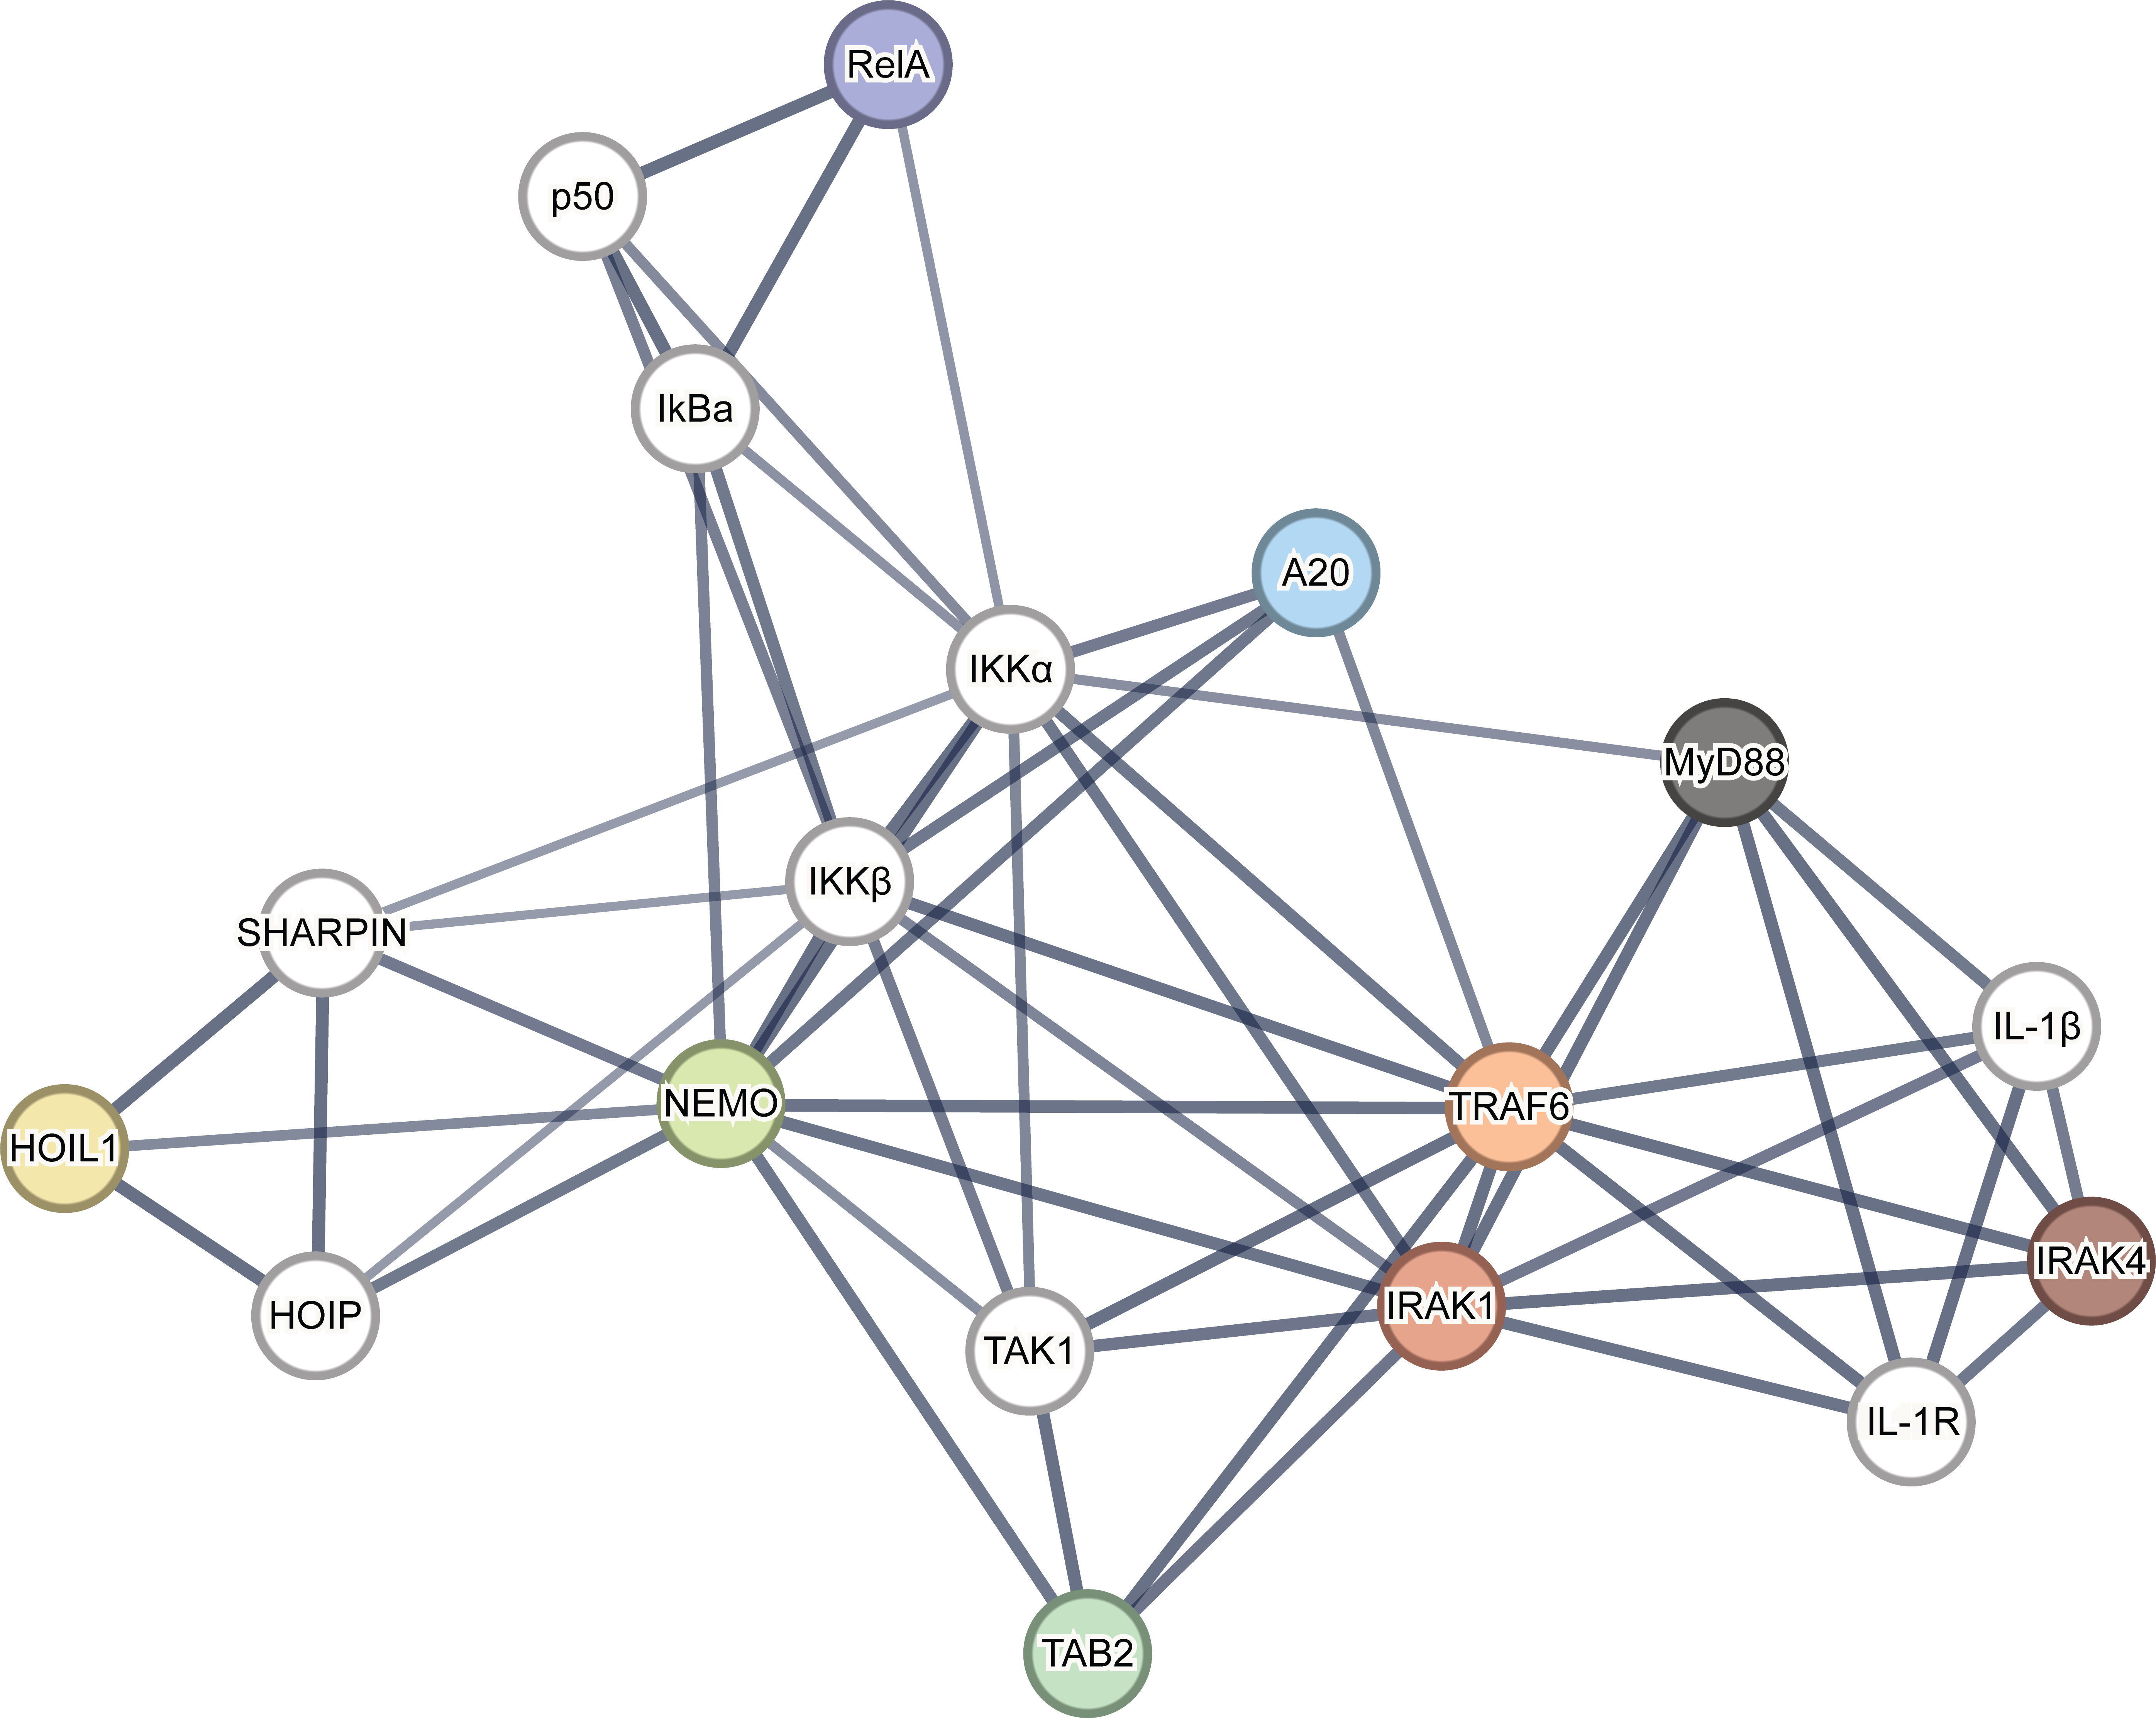
\includegraphics[width=\textwidth, height=\textheight, keepaspectratio]{img/interactome.png}}
\captionsetup{parbox=none}
\captionof{figure}[The IL1{\textbeta}-induced NF-κB signaling pathway interactome]{\textbf{The IL1{\textbeta}-induced NF-κB signaling pathway interactome.} Physical complex network with edge weights indicating the link confidence. Minimum interaction score for linkage is 0.7 (high confidence). Focus proteins are shaded. (Created by the thesis author using string-db.org\autocite{Szklarczyk_2019}}
\label{img:interactome}
\end{centering}
 
For cells, the input is IL-1 ligand and the outputs are NF-κB, MAPK and other transcription factors. Yet, observing the circuitry wiring live through microscopy is an endeavor that has not been undertaken before. Without it, it would be unknown what intermediary steps the IL-1 pathway proteins take to transduce its signal from MyD88 to NF-κB. To help form a more cohesive picture of the pathway, I will survey proteins from several complexes to establish how these proteins cause dynamic changes to each other to produce an output. Focus proteins and my hypothesized pathway assembly order is shown in the figure below (Fig.~\ref{img:pathway}). My hypothesis is that the first complex to assemble is the Myddosome, followed by TRAF6, the TAK1 complex, LUBAC (perhaps simultaneously with the Myddosome or with TRAF6-TAK1 complex), the IKK complex, NF-κB, and lastly, A20. I also hypothesize that once the pathway assembles, it will disassemble. How it disassembles could be a top-down or bottom-up approach. Because the A20 deubiquitinase is recruited by NEMO \autocite{Zhang_2000}\autocite{Mauro_2006}, I hypothesize that disassembly will start with the deubiquitination of the IKK complex and culminate with the Myddosome. However, given the opposing ligase action of NEMO \autocite{Laplantine_2009}, I hypothesize that a critical amount of A20 must be reached before the effects of disassembly are detectable.


\begin{centering}
\centering{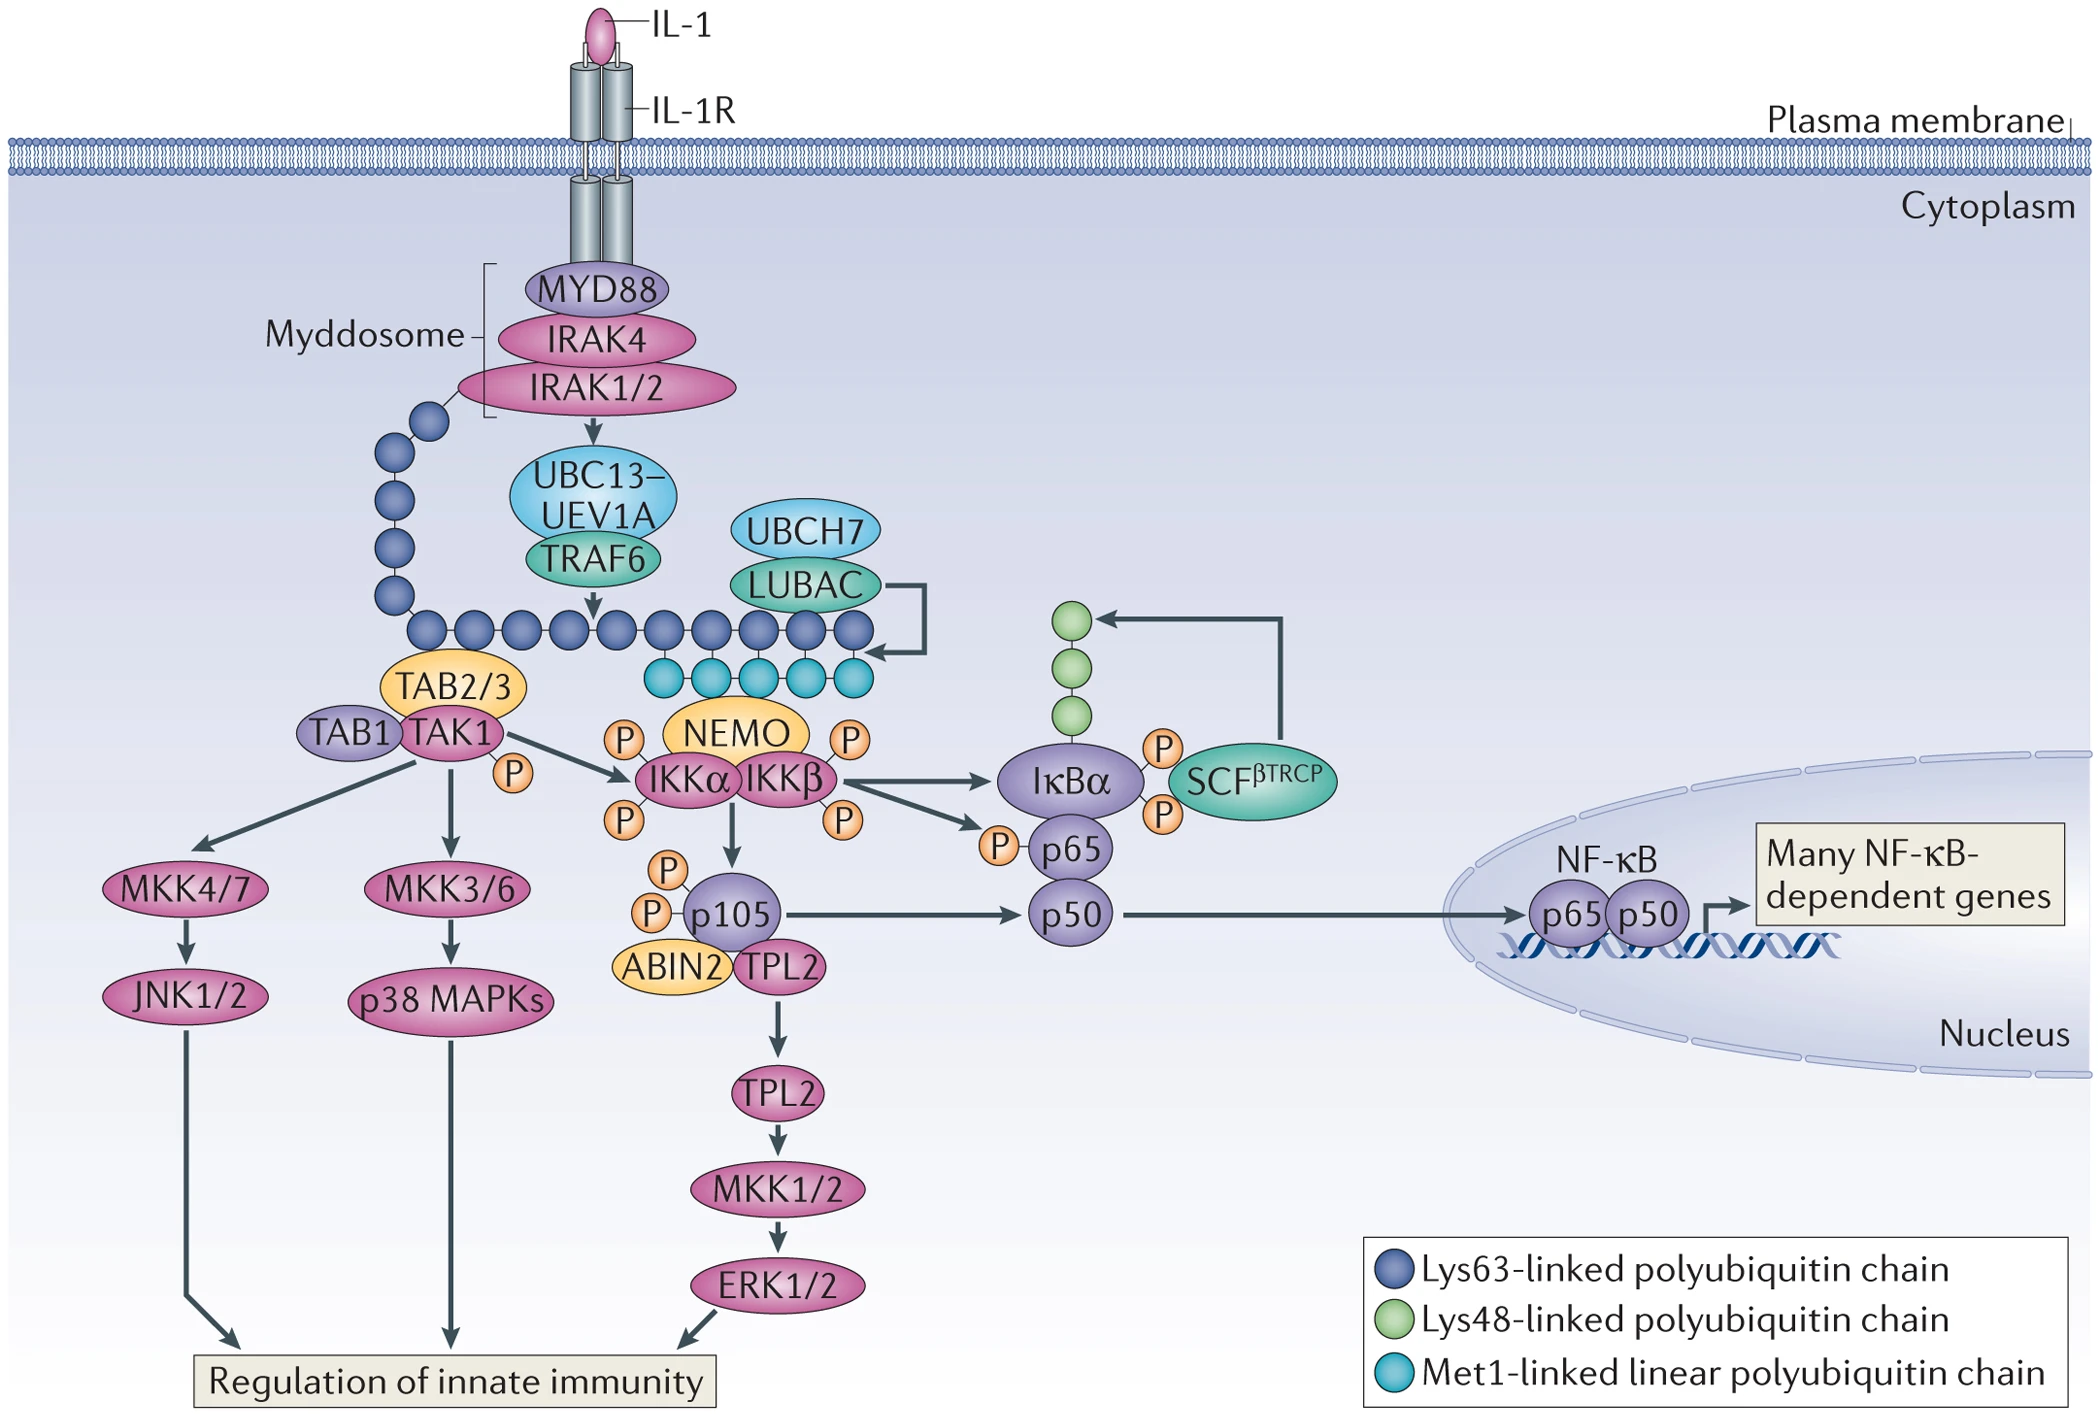
\includegraphics[width=\textwidth, height=\textheight, keepaspectratio]{img/pathway.png}}
\captionsetup{parbox=none}
\captionof{figure}[The IL-1 pathway]{\textbf{The IL-1 pathway.} The proinflammatory cytokine IL-1 induces the activation of the IL-1R signaling pathway involving a series of proteins as shown here. The IL-1R pathway culminates with the activation of NF-κB, MAPK/ERK and JNK. (Image from \autocite{Clark_2013}}
\label{img:pathway}
\end{centering}
% \autocite{Clark_2013}
 
\chapter{Methods applied}
\label{chapter:methods_applied}
\section{EL4.NOB-1, a murine lymphoma cell line}
\label{section:EL4}
\sectionmark{EL4}
The EL4.NOB-1 cell line, hereafter referred to as EL4, is a murine lymphoma cell line that has been extensively used to model the IL-1 pathway because of its known high responsiveness to IL-1 \autocite{ONeill_1990}\autocite{Boraschi_1996}\autocite{Higgins_2020}. This T-cell cell line was isolated from 9,10-dimethyl- 1,2-benzanthracene induced lymphomas on C57BL/6 (Black6) mice \autocite{Ng_2018}. EL4 has been used to study T-cell biology, immune responses, tumors, and immunotherapy. Within immune responses, it has been used to measure T-cell activation, cytokine production and cytotoxicity \autocite{Siese_1999}. To investigate IL-1 induced Myddosome assembly, I employed EL4 cell lines.

The advent of advanced gene editing technology has unlocked the capability of inserting reporter fluorophores at the endogenous loci, which permits fusion protein expression nearer to physiological conditions. Leveraging this technology, this study aims to provide unprecedented insights into the physiology of IL-1 pathway proteins.

\section{Total internal reflection fluorescence microscopy selectively visualizes surface dynamics}
\label{section:TIRF}
\sectionmark{TIRF-M}
The Myddosome assembles at the cell surface \autocite{Lin_2010}\autocite{Latty_2018}. However, conventional fluorescence microscopy cannot distinguish cytosolic MyD88 from surface MyD88 (Fig.~\ref{img:TIRF}A). To study surface dynamics, a microscopy technique that selectively illuminates the plasma membrane is required.
 
Total internal reflection (TIR) is an optical phenomenon that occurs when light traveling through one medium encounters another medium with a higher refractive index. At a specific angle of incidence called the critical angle, light is entirely reflected back into the first medium instead of being transmitted to the second medium (Fig.~\ref{img:TIRF}B). This reflection is known as total internal reflection \autocite{Axelrod_1984}. TIR occurs under certain conditions: (1) the incident light must travel from a medium with a low refractive index to one with a higher index, and (2) the angle of incidence must be greater than the critical angle. Generally, the critical angle is oblique. As the angle of incidence approaches the critical angle, the reflected light becomes increasingly polarized, enhancing the amount of reflected light. Beyond the critical angle, interference occurs, superimposing the light and generating light and dark fields \autocite{Axelrod_1989}\autocite{Axelrod_2008}. A notable property of TIR is the generation of evanescent waves that propagate parallel to the interface, decreasing exponentially as they move further from the interface. These evanescent waves can excite fluorophores near the interface. This property has been exploited in biology with a technique called total internal reflection fluorescence microscopy (TIRF-M), allowing visualization of events near the cell surface with high spatiotemporal resolution. The penetration depth of TIRF-M is approximately 100 nm \autocite{Fish_2022}, enabling exclusive visualization of surface dynamics, such as IL-1 receptor signaling.
 
Two methods can achieve TIRF: one involves a prism to direct light at an angle, while the other uses the objective lens to illuminate the peripheral field of view. Prisms offer more even illumination \autocite{Fish_2022}. The inverted microscope approach is more common because it is easier to implement and more stable. The objective lens illuminates and captures the secondary light emitted from interacting fluorophores.
 
\begin{centering}
\centering{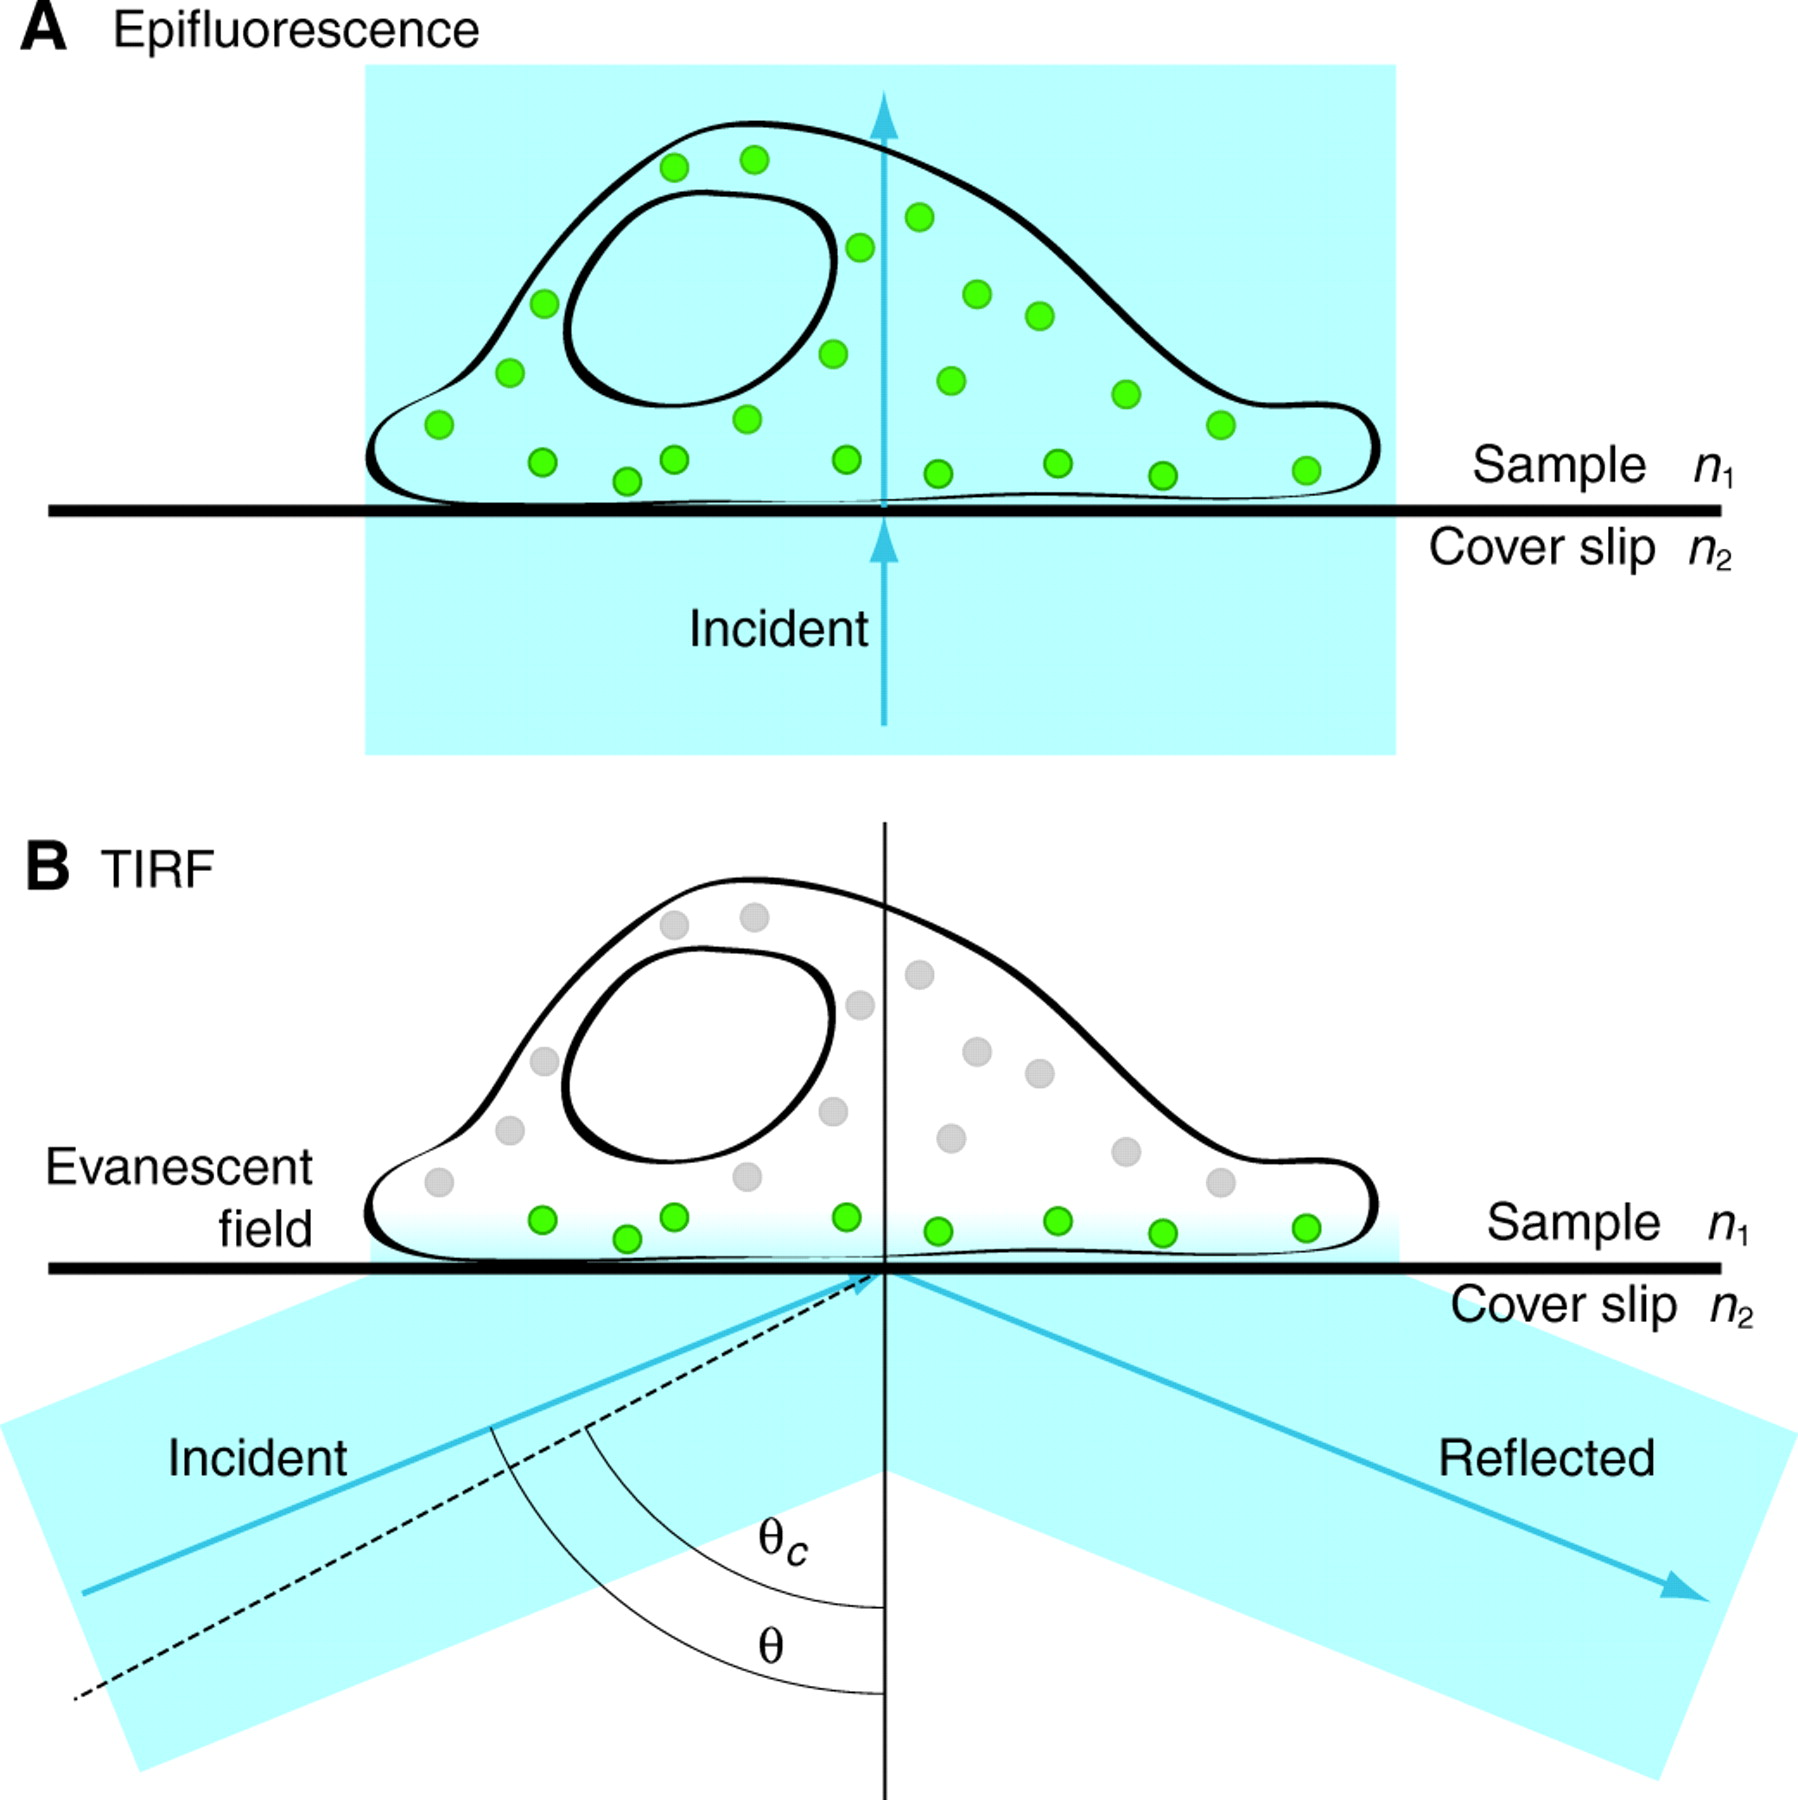
\includegraphics[width=\textwidth, height=\textheight, keepaspectratio]{img/TIRF.jpg}}
\captionsetup{parbox=none}
\captionof{figure}[TIRF microscopy limits light penetration depth]{\textbf{TIRF microscopy limits light penetration depth.} The physics of the glass-medium interface in (A) epifluorescent and (B) TIRF microscopes.
\\
\\
(A) Epifluorescent microscope. Light illuminates the entire sample.
\\
\\
(B) Total internal reflection fluorescence (TIRF) microscope. Light enters at an incident angle (θ) greater than the critical angle (θc). Excitation light is reflected with some light entering the interface as an evanescent wave. Only a few fluorophores are excited (green circles).
\\
\\
Figure from \autocite{Mattheyses_2010}.}
\label{img:TIRF}
\end{centering}
 
TIRF-M has additional benefits for cell biology. It not only limits the field of view to events near the cell surface but also removes background fluorescence outside of this range (Fig.~\ref{img:TIRF_comparison}). Furthermore, it reduces cell phototoxicity \autocite{Fish_2022}. Beyond cells, TIRF-M has been widely used in biochemistry to visualize single molecules and measure protein kinetics, as the reagents would be outside the field of view \autocite{Axelrod_2001}\autocite{Boehm_2016}. Similarly, TIRF-M can address surface biochemistry questions. For instance, TIRF-M can determine the duration of a fluorophore's presence at the cell surface \autocite{Leake_2006}\autocite{Boehm_2016}. I will use TIRF-M to measure the dynamics of IL-1R signaling proteins since they are proximal to the cell surface.
 
\begin{centering}
\centering{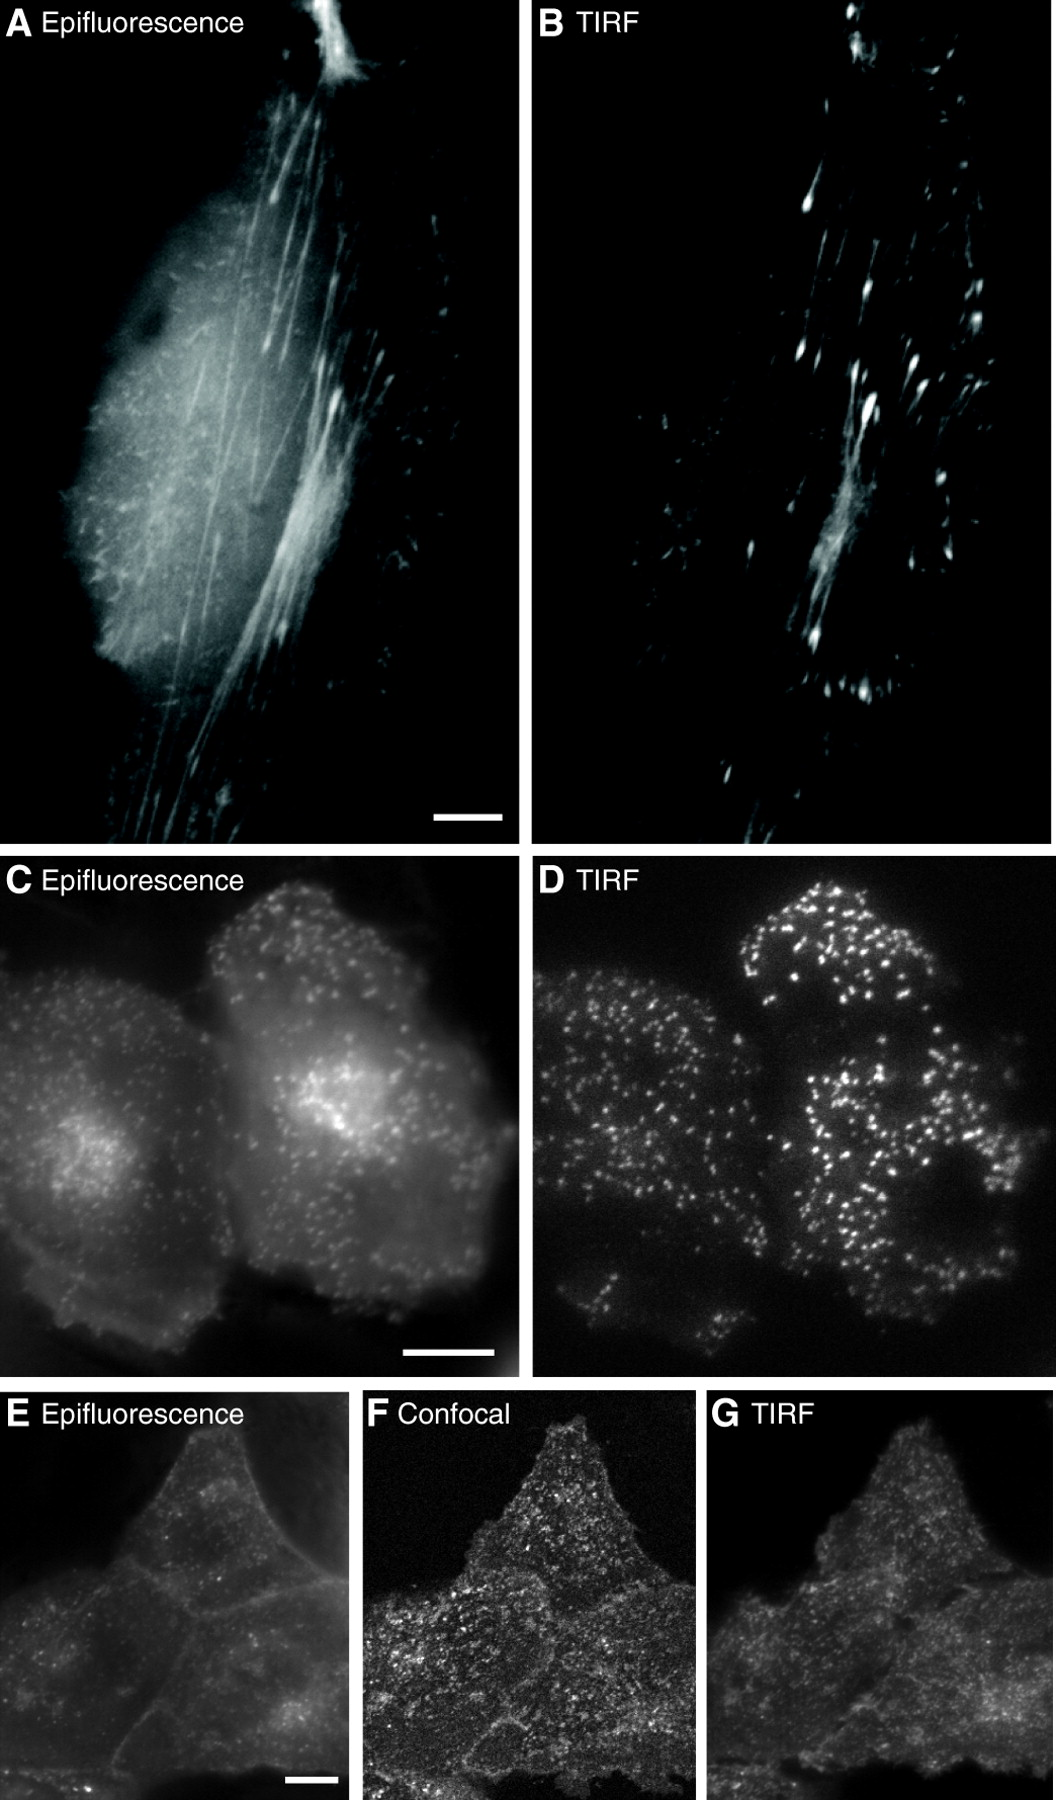
\includegraphics[width=\textwidth, height=\textheight, keepaspectratio]{img/TIRF_comparison.jpg}}
\captionsetup{parbox=none}
\captionof{figure}[Sample illumination is different between epifluorescence and TIRF microscopy]{\textbf{Sample illumination is different between epifluorescence and TIRF microscopy.}
\\
\\
(A, B) Actin (LifeAct-GFP) in Madin-Darby canine kidney cells.
\\
\\
(C, D) Clathrin (clathrin light chain--GFP) in HeLa cells.
\\
\\
(E-G) Caveolin-1 (caveolin-1-eGFP) in Madin-Darby canine kidney cells.
\\
\\
Scale bars: 10 μm. (Figure from \autocite{Mattheyses_2010}.)}
\label{img:TIRF_comparison}
\end{centering}
 
A limitation of TIRF-M is scattered light, which may originate from the distance to the glass-medium interface. The further from the interface, the more likely the observed light is scattered. The cell's composition, including collagen, can also be a source of scattered light \autocite{Axelrod_2021}. To eliminate the effects of scattered light in images, a common approach is to estimate the cytosolic background using a median filter \autocite{Kalaidzidis_2019}. To implement this technique, I have developed a pipeline that subtracts the median filter from the experimental images, resulting in background-reduced images. For further details, please refer to the Methods section in Chapter~\ref{chapter:PIRATES_PARLEYS}.
 
\section{Supported lipid bilayers reconstitute cell-to-cell interactions}
\label{section:SLB}
\sectionmark{Supported lipids}
The ligand is essential for activating the IL-1 pathway. However, introducing ligand directly into the medium prematurely activates cells before they can be visualized, which had been a limitation in previous studies \autocite{Latty_2018}. Because of this approach, the field does not know the initial steps of MyD88 oligomerization. Furthermore, the activation would not be localized if the ligand were added to the medium before imaging. To restrict receptor activation to the interface while controlling the timing of activation, one viable approach is to incorporate the ligand into the glass surface. Supported lipid bilayers (SLBs) are stable artificial phospholipid bilayers similar to the plasma membrane which are formed on top of a flat solid support, in our case, glass. Their preparation is detailed in \autocite{Grakoui_1999}.

Supported lipid bilayers (SLBs) have been effectively employed in vitro for reconstituting membrane dynamics on glass surfaces \autocite{Groves_2003}. By integrating SLBs with total internal reflection fluorescence microscopy (TIRF-M), researchers have functionalized these SLBs to examine immune receptor signaling \autocite{Grakoui_1999}\autocite{ODonoghue_2013}\autocite{Taylor_2017}\autocite{Hui_2019}. I will use SLB to investigate the signal transduction of interleukin-1 (IL-1) in living cells. With SLBs, I can selectively visualize IL-1 receptor dynamics, and elucidate the initial steps of Myddosome assembly, which were unknown \autocite{Latty_2018}.

\section{Phase portrait analysis and its application to protein colocalization}
\label{section:pp}
\sectionmark{Phase portraits}
A dynamic system evolves over time and often exhibits complexity due to multiple interacting variables that produce non-linear responses. The IL-1 pathway is a highly dynamic system \autocite{Latty_2018}\autocite{Deliz-Aguirre_2021}, making the temporal evolution of signaling events and its protein interactions a challenge for dynamical systems.
 
To study complex dynamical systems, a mathematical framework is often employed, which is referred to as systems biology in the biological context \autocite{Wolkenhauer_2005}. Control theory, an engineering field, considers systems as circuits, addressing regulation, feedback, and loops \autocite{Kitano_2002}. These two fields are closely related, and I leveraged their applied mathematics frameworks to decipher the assembly of nine proteins in the IL-1 pathway.
 
Phase portrait analysis is an analytical tool often employed to disentangle complex dynamic systems. It involves the graphical representation of data plotted in phase space, a plot of system variables that maps all possible states of a system. Trajectories are subsequently drawn, and the average change (derivatives) between variables can be determined for all given states. For the IL-1 signaling pathway, phase portrait analysis can be useful for identifying which protein stoichiometry is most stable (the equilibrium point) and how two proteins affect each other’s dynamic (feedback). The shape of the phase portrait can be used to make predictions of the colocalization dynamics of puncta through mathematical modeling, which typically involves differential equations such as predator-prey models. Recently, phase portrait analysis was used to discover the chemical basis of the contraction of the actomyosin cortex in \emph{Caenorhabditis elegans} \autocite{Yan_2022}.
 
\subsection{Predator-prey phase portrait}
\label{subsection:predator_prey}
In its simplest form, rabbit population growth can be modeled as $N(t) = N_0 \cdot e^{rt}$ where
\begin{itemize}
\item $N(t)$ is the population size at time $t$,
\item $N_0$ is the initial population size at $t = 0$,
\item $e$ is the base of the natural logarithm, $\approx 2.72$,
\item $r$ is the growth rate, and
\item $t$ is the time.
\end{itemize}
A simple log-transformation linearizes the population growth. However, introducing predators such as wolves makes the prey (rabbits) population growth dynamics more challenging to predict.

A century ago, scientists faced a similar challenge when Vito Volterra observed oscillatory behaviors in fish population dynamics following predation (example in Fig.~\ref{img:lotka_volterra}A). Independently, Alfred Lotka investigated a similar question involving plants and herbivores. Lotka and Volterra successfully resolved the predator-prey population conundrum by developing a set of equations now known as the Lotka-Volterra equations (history described in \autocite{Ginoux_2017}). Volterra used phase portrait analysis to visualize population trajectories, which helped him discover the population dynamics equations he formulated. The Lotka-Volterra phase portraits are orbital and resemble the letter “D,” depicting the growth of prey population followed by predator population growth (Fig.~\ref{img:lotka_volterra}B). Subsequently, the prey population declines, followed by a collapse of the predator population. This cycle then repeats (Fig.~\ref{img:lotka_volterra}A). A similar approach has been used to examine protein colocalization dynamics on the smaller mesoscale \autocite{Yan_2022}.

\begin{centering}
\centering{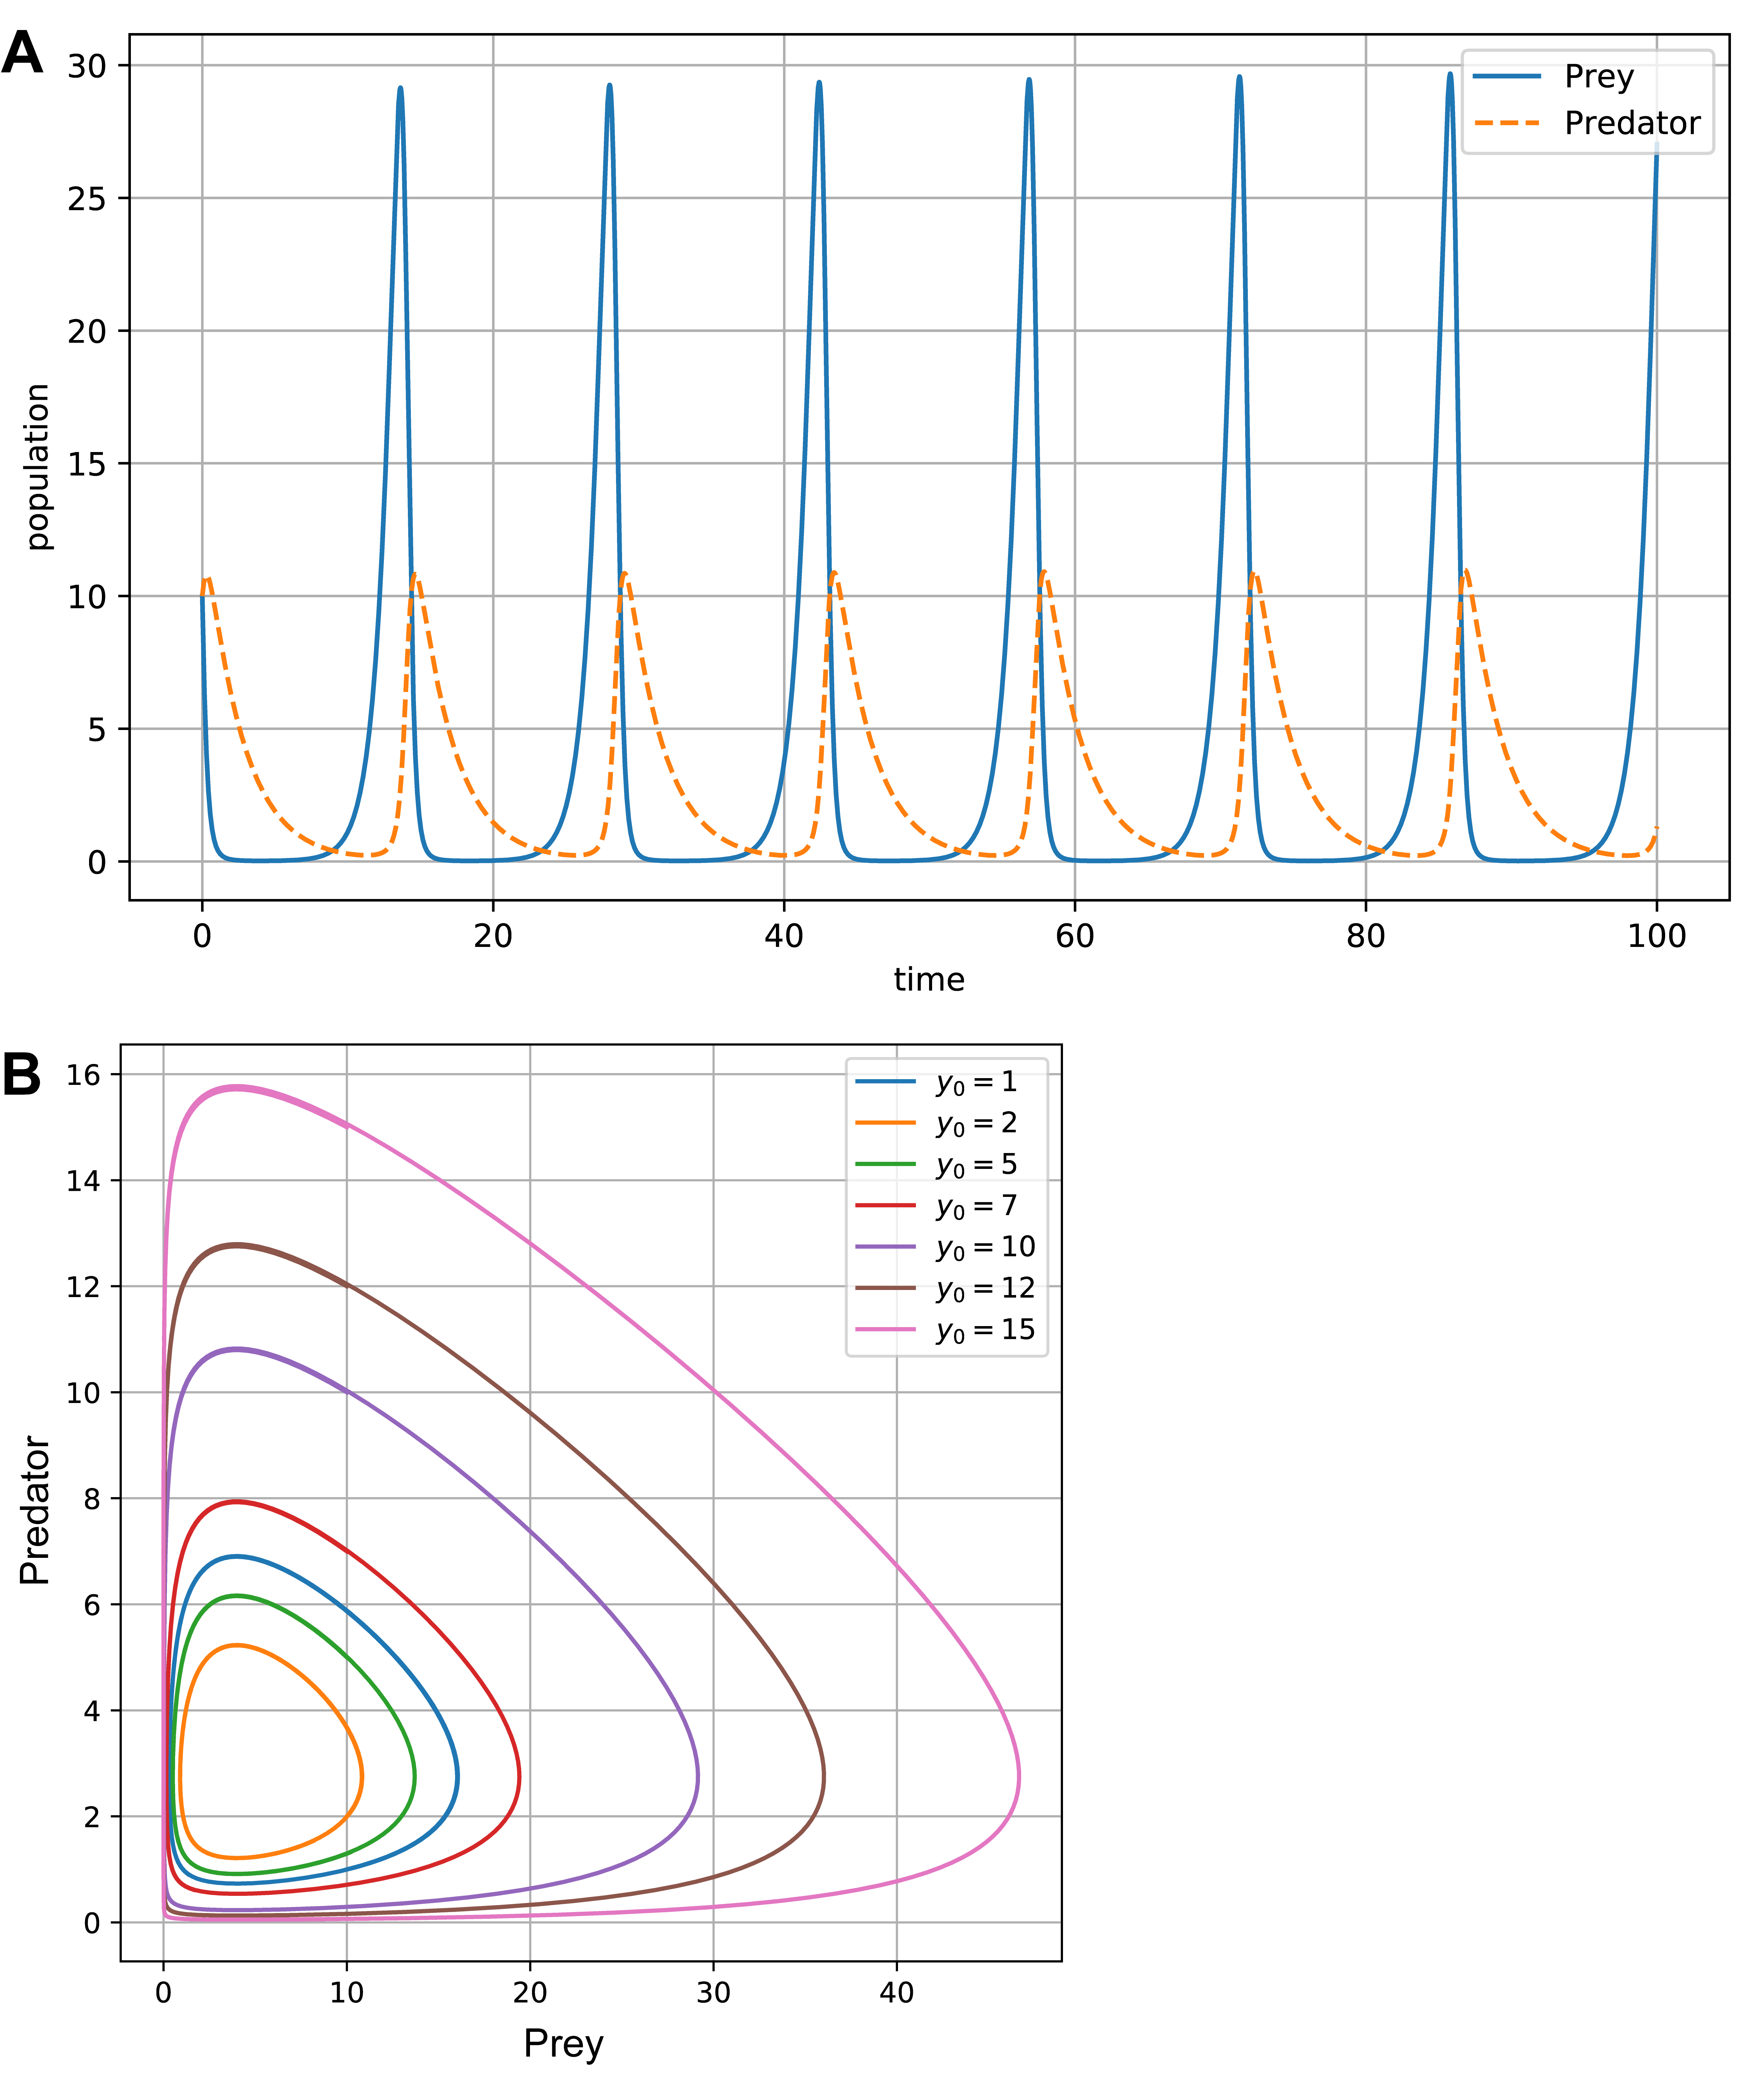
\includegraphics[width=\textwidth, height=\textheight, keepaspectratio]{img/lotka_volterra.png}}
\captionsetup{parbox=none}
\captionof{figure}[Lotka-Volterra predator-prey model]{\textbf{Lotka-Volterra predator-prey model.}
\\
\\
(A) Phase line showing the predator and prey population over time.
\\
\\
(B) Sample phase portraits with different parameters \autocite{wiki:Lotka–Volterra_equations}.}
\label{img:lotka_volterra}
\end{centering}

\section{Protein modules are an emerging level of biochemical organization}
\label{section:modularity}
\sectionmark{Modularity}
Cells must recognize various inputs and generate similar outputs \autocite{Alberts_2002}. However, biologists often wonder how biological complexity arises from a limited set of proteins \autocite{Hyman_2011}. One approach is to use interchangeable parts \autocite{Alcala-Corona_2021}. Evolutionary biology has proposed the concept of modularity to explain protein diversity \autocite{Wagner_2007}. Cellular modularity suggests that the complexity of logical systems in cells can be simplified into functional components called modules \autocite{Alcala-Corona_2021}. The concept of modularity was first put forward by Tony Pawson and colleagues in 1986 when they found that Src homology 2 (SH2) could recognize various phosphorylated proteins \autocite{Sadowski_1986}. Later, his lab and others showed SH2 domains in oncogenic kinases, scaffolds and adaptor proteins. The universality of the SH2 pathway paved the way to modular biological organization \autocite{Scott_2013}. Modules are typically defined in terms of protein domains \autocite{Pawson_1995}\autocite{Bashton_2007}. Modularity is now viewed as circuits with read, write, and erase functions \autocite{Mayer_2017}. However, a module’s actual function depends on its position within the cell’s larger network, as it can be structural or functional \autocite{DelVecchio_2015}\autocite{Dobay_2018}. A similar biological control systems approach may be used to understand the IL-1 pathway's regulatory circuitry. Modularity may not be limited to domains, but rather, it may extend to protein complexes themselves. Indeed, TRAF6 has been shown to be a modular protein that helps bridge diverse pathways \autocite{Wu_2003}\autocite{Naismith_1998}. Similarly, the Myddosome is a module shared by the TLR and IL-1 signaling pathways \autocite{Rosadini_2015}.
 
Modules extend in time, and their activity can control their function \autocite{Callebaut_2005}. Dynamic modularity implies that functional decomposition does not always account for cellular behavior \autocite{Slusarczyk_2012}. This suggests that \emph{in vitro} reconstitution experiments may not accurately reproduce in vivo dynamics. To understand regulation, utilizing cell lines would be a more suitable approach.
 
The concept of modularity has spread to other biological disciplines such as synthetic biology \autocite{DelVecchio_2015} and systems biology \autocite{Wagner_2007}. In synthetic biology, modularity has been applied to program cells with \emph{de novo} functions using genetic engineering \autocite{Bashor_2010}\autocite{Lim_2022}. In systems biology, modules have been employed to understand networks (Del Vecchio et al., 2008). However, synthesizing new biological modules is challenging due to codependence, unintended interactions, and circuit load affecting dynamics (Del Vecchio et al., 2016). Understanding the IL-1 pathway's regulatory meshwork can aid in developing therapeutics that restore homeostasis.
 
Modularity is hypothesized to occur in innate immune pathways \autocite{Tan_2019}. Immune proteins reorganize in various ways to create diverse cellular structures and functions \autocite{Tonegawa_1983}\autocite{Chaplin_2010}. One type of structure which cells use for signaling are called signalosomes. Signalosomes are large, multi-protein signaling complexes that condense \autocite{Bray_1995}. In innate immunity, functionally similar self-oligomerizing structures called Supramolecular Organizing Centers (SMOCs) have been identified \autocite{Kagan_2014}, a type of signalosome. These structures employ common oligomeric structures but exhibit distinct biochemical functions. SMOCs like the Myddosome are one example of domain modularity in biology \autocite{Kagan_2014}\autocite{Tan_2019}. This thesis will explore one example of how proteins achieve comparable signaling outputs from diverse inputs.

The orchestration of an immune response is determined by complex decision making in signaling cascades \autocite{DeFelice_2019}. The decisions may play a role in grading inputs to produce digital and analog outputs \autocite{Cao_2023}. But a critical yet enigmatic part of this puzzle lies within the IL-1 pathway regulation. While protein interactors have been identified, the regulatory mechanisms that lead to decision-making remain elusive. The numerous known interactors of the IL-1 pathway call for a comprehensive review of the dynamics to unveil possible feedback mechanisms of the involved proteins.

\chapter{Aims of the study}
\label{chapter:aims}
\chaptermark{Aims}
\sectionmark{}
Focusing on key IL-1 pathway proteins MyD88, IRAK4, IRAK1, TRAF6, TAB2, HOIL1, NEMO, RelA and A20, this thesis aims to revise the central question: How does the extracellular recognition of IL-1 transform into a controlled yet proportionate cellular response that achieves a decisive cellular outcome through nine key proteins?

To answer this, the focus was on investigating, at the single-molecule level, how cells convert individual behaviors of molecules and complexes in the IL-1 pathways into a highly regulated signaling response.
 
In contrast to previous methodologies, this thesis will use quantitative high-spatiotemporal resolution microscopy to visualize the molecular dynamics of the IL-1 pathway in live cells expressing fluorescently labeled pathway proteins. By integrating TIRF microscopy with supported lipid bilayer technology and high-throughput image analysis, the discrete stages and reactions that govern the transduction of information through the IL-1 pathway can be investigated. More specifically, I will investigate the assembly and disassembly dynamics of the IL-1 pathway.
 
Current technology enables the quantification of single cells with single-molecule resolution near physiological conditions. The widespread availability of CRISPR/Cas9 technology allows for gene editing to insert fluorescent tags at endogenous gene loci, minimizing overexpression artifacts associated with gene-editing strategies prior to CRISPR/Cas9. Additionally, improvements in the quantum efficiency of CMOS sensors permit rapid measurements of single molecules over extended periods of time. Current software supports the detection and tracking of puncta over time, while increasingly fast high-performance computers facilitate the deployment of high-throughput image analysis pipelines. By combining these tools, the IL-1 pathway protein dynamics images can be quantified at an unprecedented scale.

\section{Aim 1: Investigating the Role of MyD88 Oligomer Size in the IL-1 Pathway}
\sectionmark{MyD88 Size Role}
In the first part of this thesis, I will combine different technological approaches to examine how IL-1 transduces signals through the Myddosome. I will explore the dynamic nature of MyD88, assess the colocalization requirements of Myddosome proteins, and determine recruitment times. Additionally, I will investigate the functions of IRAK4 and IRAK1 through genetic knock-outs.

\section{Aim 2: Decoding the Regulatory Circuitry of the Assembly and Disassembly of IL-1 Pathway Proteins}
\sectionmark{IL-1 Circuitry}
In the second part of this thesis, I will expand this assay to study the molecular dynamics of IL-1 pathway proteins, from the Myddosome to the NF-κB complex. Because a high-throughput method to quantify puncta dynamics in live cells does not exist,\footnote{FIJI \autocite{Schindelin_2012} and TrackMate \autocite{Tinevez_2017} functionality is limited in HPC environments} I will create a completely new image analysis pipeline. By applying phase portrait analysis to a newly generated large dataset, I aim to detect novel and previously undiscovered positive and negative feedback loops within the IL-1 pathway. Utilizing modular network theory from biological control systems, I will infer the module(s) that constitute the IL-1 pathway. Since the pathway disassembly mechanism remains unknown, I will investigate how the pathway proteins disassemble. My approach was able to resolve molecular details of disassembly, and ascertain which disassembly model is correct.
 
In summary, the overarching goal of this thesis is to leverage big data to comprehend the molecular mechanisms that regulate IL-1 activated Myddosome assembly and its signal transduction. These regulatory mechanisms are crucial for ensuring a controlled yet decisive inflammatory response capable of clearing threats to restore homeostasis.

\mygeometry
\part{Methods}
\restoregeometry
\chapter{Stoichiometries from images: Puncta quantified with a custom image analysis pipeline}
\label{chapter:pipeline_v1}
\chaptermark{Pipeline v1}
\section{Experimental assay}
\label{section:assay_v1}
Cell culture, gene editing, assays, imaging, data acquisition, statistical analysis, staining, and validation is described in \autocite{Cao_2023}\autocite{Deliz-Aguirre_2021}. 

To decode how the Myddosome assembles, I analyzed the dynamics of MyD88-eGFP in cells that had been activated with the aforementioned SLB system (Fig.~\ref{p1:1}A, microscopy data generated by Mariam Chupanova, Marcus Taylor and myself).

I observed that after a few minutes of cell contact with the SLB, MyD88-eGFP is recruited to the cell surface and forms puncta (Fig.~\ref{p1:3a}A). Initially, these MyD88-GFP puncta were dim and transitory (Fig.~\ref{p1:3a}). Over time, I observed that some puncta became brighter and stable (Fig.~\ref{p1:3a}).

Previous imaging experiments had shown that these MyD88-GFP puncta colocalized with fluorescently labeled IL-1 tethered to the SLB (data acquired by Marcus Taylor) (Fig.~\ref{p1:1}B). Based on this observation, I hypothesized that a portion of these MyD88-GFP puncta are fully assembled Myddosome complexes, and that smaller, dimmer and transitory puncta represent the nucleation and oligomerization of MyD88---the initial stage of Myddosome assembly.

The existence of intermediary steps in Myddosome assembly is unknown. To understand and quantify these intermediary steps, I developed an analysis pipeline that used particle tracking to identify MyD88-GFP puncta within the high spatiotemporal resolution imaging of live cells.

We took images using a sCMOS camera. To remove the camera’s dark-current noise, I captured over a thousand images with the shutter closed at the same exposure as the experimental images. Then, I subtracted the average of these thousand frames from the experimental images.

To minimize the contribution of background fluorescence intensity to measurements of puncta intensity, I passed TIRF-M images through a median filter to estimate background fluorescent intensity across the entire image. This estimated background was subtracted from the image.

Using the TrackMate particle tracker \autocite{Tinevez_2017}, I extracted the fluorescence intensity of MyD88-GFP puncta. The resulting brightness measurements would be in arbitrary units, and offer no stoichiometric insights. Stoichiometric measurements would allow us to compare our live cells to the stoichiometry (oligomer length) of purified Myddosomes \autocite{Lin_2010}.

I calibrated the TIRF-M fluorescence measurements with monomeric GFP. This allows signal normalization, and offers insights into the stoichiometry of individual MyD88 puncta. It also allows me to compare the images captured on different dates. Now, I have a system which lets me estimate MyD88 copy numbers from individual puncta. I can finally compare the fluorescent measurements to the biochemically-determined stoichiometries \autocite{Lin_2010}\autocite{Moncrieffe_2020}.

The image analysis pipeline also enables assaying the kinetics of MyD88 assembly and quantitatively identify intermediate stages of Myddosome assembly (full detail of image analysis pipeline see Methods, “Image analysis pipeline v.1”).


\begin{centering}
\centering{\includegraphics[height=\textwidth, width=\textheight, angle=-90, keepaspectratio]{jcb/Workflow.png}}
\captionsetup{parbox=none}
\captionof{figure}[short caption]{\textbf{Pipeline workflow.}
\\
\\
(1) Images are converted to TIFF. The background is removed.
\\
\\
(2) Images are segmented using the MyD88 channel.
\\
\\
(3) Cells are cut out of the original image and made into substacks. Then, puncta are tracked with TrackMate.
\\
\\
(4) Intensities are extracted with MATLAB.
\\
\\
(5) The MATLAB tables are converted to CSV and in a style which R can read.
\\
\\
(6) The area and background intensity of cells measured by ImageJ are combined into one table.
\\
\\
(7) The puncta are colocalized using a MATLAB script.
\\
\\
(8) The data is analyzed and plots are made using the aforementioned tables.}
\label{fig:p1M}
\end{centering}

\section{Pipeline for analyzing the protein dynamics images}
\label{section:pipeline_v1}
\sectionmark{Dynamics Pipeline v1}
Results~\ref{chapter:p2} uses the \emph{Dynamics Analysis Pipeline}. Its scripts and guides are available at \\ \url{https://github.com/MJ-Taylor-Lab/myddosome-dynamics-pipeline}. The description is available at \autocite{Deliz-Aguirre_2021}.

The pipeline has eight steps:
\begin{enumerate}

\item \textbf{01\_TIFF-Subtract.ijm}. Runs on ImageJ.

\begin{itemize}

\item TIFF is the gold standard scientific image format. The microscope produces proprietary ND2 files which includes a TIFF image plus metadata. This script first splits the 16-bit TIFF stack and metadata from the ND2 files. It then splits channels into different TIFF files. This script is also used to remove the background intensity emanating from dark-frame noise, and the non-specific cytosolic fluorescence. 

\item The camera generates noise from a variety of sources that include dark current, read noise, and thermal noise, as well as photon based response noise like the gain and the flatfield \autocite{Diekmann_2022}. To correct for the dark current noise and the fixed pattern noise, I generated a dark-frame of the camera noise. This frame is generated first by closing the camera shutter and acquiring several (5000 in our case) frames at the same exposure as the experimental images. Then, these frames are mean-averaged. Lastly, this average image is subtracted from the “experimental” and “calibration” images.

\item Cells have autofluorescence, and this could impact the measurements. The non-specific cytosolic fluorescence was estimated using a median filter. Median filters are edge preserving, thus the estimate is symmetric to the cell, retaining the proportions seen. The background was calculated for a 25-px (approximately 3.67 µm) radius. This radius size should roughly correspond to the cell radius.

\end{itemize}

\item \textbf{02\_Segmentation.ijm}. Runs on ImageJ. I segmented the images so that biological replicate measurements exist within an image. This script segments cells using a marker-controlled watershed segmentation (available as a plugin called MorphoLibJ\autocite{Legland_2016}. This script uses a maximum projection of the channel of the reference protein, blurs and dilates it to serve as the marker. It also blurs and erodes the maximum projection image to capture the marker.

\item \textbf{03\_Substacks-TrackMate.ijm}. Runs on ImageJ. 

\begin{itemize}

\item To accelerate the cell analysis, I made substacks from the segmented cells. I already had two stacks, a dark-frame stack for tracking puncta, and a median subtracted substack for obtaining the intensities.

\item From the segmented cells, I calculated the area and brightness.

\item The last step was to track the puncta on the dark-frame subtracted image substacks. I used the TrackMate plugin \autocite{Tinevez_2017}.

\end{itemize}

\item \textbf{04\_Reextracintensities/ReextractIntensities\_04.m}. Runs on MATLAB using a modified script adapted from \autocite{Taylor_2017}. I now have the puncta coordinates, but not the fluorescent intensities. To extract the intensities from the median image, I first extracted the TrackMate coordinates from its XML file output. Then, I segmented a 3\times3 pixel box with sub-pixel localization. Lastly, I extracted the summed intensity from that box and exported it as a table.

\item \textbf{05\_MATLAB-CSV.R}. Runs on R. The MATLAB table was adapted to run on R. with x, y, t, intensity and track ID columns.

\item \textbf{06\_Area-Background.R}. Runs on R. To analyze images on R (later described under 08\_Analysis), I made an output list that lists cell tables, their paths, area and intensity.

\item \textbf{07\_Colocalization/run\_trackmate\_anaylsis.m}. Runs on MATLAB using a modified script adapted from \autocite{Taylor_2017} with coding contributions from Alexander Schmidt (Taylor Lab). For the IRAK4/1 images, we took images of the GFP and mScarlet channels. They were tracked, but separately. Because I was interested in the interplay between proteins, I needed to calculate colocalization. I had three criteria: (1) maximum distance cutoff, (2) minimum association time, and (3) minimum dwell time of the puncta. After this, I generated an output table to be later analyzed in R.

\item \textbf{08\_Analysis}. The last step was the analysis and plotting of the data. Several parameters were calculated for each track, including their dwell time, maximum brightness and intensity change from start to max. I also calculated the max size and recruitment time for the colocalized puncta.

\end{enumerate}

\section{Pipeline for analyzing the staining images}
\label{section:staining_pipeline}
\sectionmark{Staining pipeline}
To assay the level of RelA (NF-κB p65 subunit) and p38 MAPK activation in widefield images of fixed cells , I developed an image analysis pipeline. This image analysis pipeline was implemented in FIJI and R. I employed a threshold-segmentation in FIJI to identify the cytoplasmic and nuclear volume of individual cells. I segmented and identified individual cells using the MyD88-GFP and the RelA/phospho-p38 staining image. To identify the nuclear volumeI segmented DAPI nuclear stain image. The cytoplasmic volume was identified by subtracting the nuclear volume from the cell volume. I then measured the fluorescent intensity of the two segmented cellular areas. Fluorescent intensity values were then analyzed in R. First I normalized the fluorescent intensity values. For RelA I calculated the cytoplasm to nuclear ratio of RelA staining to assay nuclear translocation. For phospho-p38, I measured the nuclear staining intensity.

This analysis confirmed that gene-edited cells line expressing fluorescent protein fusion of MyD88 and IRAK4/1 can still activate a downstream IL-1 signal transduction. In conclusion, our tagging strategy did not abolish IL-1R signaling response. These cell lines can be used to investigate the dynamics of IL-1 mediated Myddosome signal transduction.

The staining images analysis pipeline is available at \\ \url{https://github.com/MJ-Taylor-Lab/myddosome-dynamics-pipeline/tree/master/StainingAnalysisPipeline}. The description is available at \autocite{Deliz-Aguirre_2021}.

\chapter{PIRATES-PARLEYS: A high-throughput image analysis pipeline that quantifies protein dynamics}
\chaptermark{High-throughput pipeline}
\label{chapter:PIRATES_PARLEYS}
My first pipeline was able to quantify the microscope images, track puncta over time and measure puncta intensities. However, the previous pipeline had a few drawbacks which I have now addressed and will be discussed below. Additionally, new techniques have been incorporated. Briefly, this new pipeline is able to run considerably faster, it requires less user involvement, and it simplifies the measuring of colocalization using a soft matter physics approach.

Currently, some of the available image analysis tools have not been optimized for live-cell (\emph{in vivo}) imaging, for example, with the cytosolic background. Other imaging tools make use of machine learning and deep learning, nowadays sometimes collectively called “artificial intelligence” (AI), which potentially introduces artifacts \autocite{Krull_2019}. My goal was to combine simple (non-AI) yet powerful image analysis techniques in a novel way to develop a completely new high-throughput (high-performance computing “supercomputer” compatible) image analysis pipeline for quantifying protein puncta dynamics as seen using live-cell fluorescent microscopy.

I used our live-cell assay as described before (Methods~\ref{section:assay_v1}). For Results~\ref{chapter:p2}, proteins were tagged in pairs: an upstream reference protein (MyD88, and TRAF6 in the TRAF6-NEMO cell line) tagged with eGFP, and a query downstream protein tagged with mScarlet. Proteins were validated as described before. Then, I proceeded to quantify the microscopy images with our new pipeline. Here, I will describe a new pipeline called Pipeline for Image analysis with Reference images, Automated Tracking, Extraction of intensities, and Segmentation (PIRATES) Phase portrait Analysis and Relative kinetics comparison Localization analysis with Extraction of data Yielding Statistics (PARLEYS), and why it was needed.

\section{Steps}
\subsection{Dark-current noise was subtracted with minimal user input}
\subsectionmark{Dark-frame}
Starting with the image acquisition, there are several camera sensor types available in the market. The most popular scientific camera sensors are charge-coupled devices (CCDs) and scientific complementary metal-oxide-semiconductor (sCMOS). CCD sensors capture less noise and are highly sensitive (they have high quantum efficiencies). However, they are slow in capturing images. By comparison, sCMOS sensors are fast, and are making leaps in quantum efficiencies nearing CCD sensors. To capture our dynamic fluorescent proteins, I opted for the fast sCMOS sensor.

Camera sensors work by converting photons into electrons. The proportion that gets successfully converted is called the quantum efficiency, which nowadays hovers around 90\%. Then, these electrons are read and converted into a number. One issue with sCMOS sensors is that they are noisy, that is, the signal fluctuates randomly. 

As with other sensitive camera sensors, one source of noise for sCMOS sensors is the dark-current, that is, thermal noise, the heat from the camera. We used liquid cooling to lower the sensor temperature down to -20ºC (253.15 K), and keep it stable (unstable temperatures can potentially produce thermal expansion whose deformations would produce shape aberrations). However, this is not enough to completely remove thermal electrons, which theoretically would need the temperature to be absolute zero (0 K) in order to have no noise. I used image processing to remove the dark-current noise.

This camera noise can be estimated by averaging several pictures with the camera shutter closed (Fig.~\ref{m:1}.1). The more frames, the better, though there is a point where capturing more images will not change the average. In my case, I overshot and took over a thousand images with the shutter closed (already at around 100 frames and 50 ms exposure, the average stabilizes), and then mean-averaged these frames (Fig.~\ref{m:1}.1). The resulting single image is called the dark-frame (Fig.~\ref{m:S1}.4 Dark-Frame).

The dark-frame exposure should be the same (or near) the experimental image exposure. This is because the higher the exposure, the higher the dark-frame intensities are because the sensor has more time to accumulate thermal electrons.

Now that I have calculated the dark-frame, and captured experimental images, I have to tell the computer which images to analyze and how. All the parameters needed to run all scripts are given by the user at this point. This is done in a single step using csv tables (Fig.~\ref{m:1}.2; Methods). It is an improvement from the previous pipeline in that the previous pipeline had eight steps that required the user to input data. Now, everything runs in a single step.

The first step the pipeline makes is converting images into standard image formats. Each pixel is an xy-coordinate, thus the fluorophore brightness detected by the camera sensor (the intensity) is saved as a matrix, typically into a tag image file format (TIFF) file. TIFF is the gold-standard scientific image format. However, our Nikon microscope produces proprietary ND2 files which includes a TIFF image stack plus metadata. To enable image processing, the pipeline first extracts the 16-bit TIFF image stack (frames set, the “video”) and metadata from the ND2 files (Fig.~\ref{m:1}.3). One drawback of the previous pipeline was that it required heavy user involvement at every single step of the way. With my new pipeline, the scripts use the image metadata to make decisions (Fig.~\ref{m:1}.3). 

The next step is removing the dark-frame. The previous pipeline removed the dark-frame from the experimental images. However now, the script automatically selects the appropriate dark-frame image. It identifies which dark-frame exposure is closest to that of the experiment. \begin{equation*}\text{dark-frame}_{\text{exposure}} = min(|\text{image}_\text{ exposure} - \text{dark-frame}_{\text{exposure}}|)\end{equation*} After, the pipeline subtracts the dark-frame from the experimental images (Fig.~\ref{m:S1}.4;~\ref{m:1}.4). The resulting image has less background noise. \begin{equation*}\text{image} = \text{image} - \text{image}_\text{dark-frame}\end{equation*}

\begin{centering}
\centering{\includegraphics[height=\textwidth, width=\textheight, angle=-90, keepaspectratio]{methods/figS1.png}}
\captionsetup{parbox=none}
\captionof{figure}[Subtracting the dark-frame removes the background noise]{\textbf{Subtracting the dark-frame removes the background noise.} For visualization purposes, I cropped a cell out of the original image so that detail can be appreciated. This cropped box measures 17.31 µm by 16.43 µm (0.1467 µm/pixel). Also for illustrative purposes, the contrast is rescaled each time using the auto-contrast function of ImageJ. While images are monochromatic, I used the viridis plasma look-up-table (LUT) because this color map offers higher visual contrast while being colorblind friendly. Then, I inverted the LUT so that the colors can be appreciated in print media. Back to the dark-frame subtraction, I first estimated the camera dark-frame, that is, the thermal noise. To estimate such noise, I captured 1000 images at the same exposure as the experimental image, but with the camera shutter closed. That way, only camera noise is captured in the images. The correct exposure time is important because the longer the acquisition, the more thermal electrons are accumulated, which translates into thermal noise. This dark-frame was subtracted from the original image.}
\label{m:S1}
\end{centering}

\subsection{Different images for different purposes: the tracking and intensity images}
\subsectionmark{Tracking, intensity mages}
My objective was to track protein puncta (spots) over time and measure their intensities. To see the protein dynamics, proteins were labeled with fluorophores, so that the proteins of interest can be selectively visualized. Thus, we used fluorescence microscopy to visualize live-cell protein dynamics. Quantitative fluorescent microscopy works by measuring light apart from the background.

To track the proteins, I need images that are excellent for tracking which must have high signal-to-noise ratios (bright puncta and dark background) for reasons that will be discussed later in this section.
\begin{equation*}
\text{SNR} = \frac{\text{signal}}{\text{noise}} = \frac{\mu_{int\text{ puncta}}}{\mu_{int \text{ background}}}
\end{equation*} 
Where $SNR$ is signal-to-noise ratio, $\mu$ is the mean, and $int$ is intensity.
The signal-to-noise ratio is a metric of how good the contrast is in an image. In this case, the signal is the brightness of the fluorophore and the background is the rest. A high signal-to-noise ratio is desirable, and there are several ways to achieve this. It can be classified as before, during or after image acquisition. Each method has its own advantages and drawbacks, but they can be combined to get a better quantifiable image, which is what this pipeline does.

Before image acquisition, one can use bright fluorophores to produce a better signal. However, there are several considerations when using fluorescent proteins. Fluorescent proteins can produce steric hindrance which would disable complexes from forming properly. In addition to trying different molecules, one way to bypass hindrance is to tag either the C or the N terminal of the protein. The fluorescent protein needs time to maturate. Therefore, experimenters need to be aware of when a protein can be visualized. Another fluorophore consideration is that when attempting multi-color imaging, the selected fluorophore emissions (light wavelength color that bounces back) should not be near (Fig.~\ref{m:S2}5). Outside fluorescent proteins, there are fluorescent organic dyes, and while they can be brighter than fluorescent proteins, dyes need to be conjugated. For our experiments, we used eGFP and mScarlet.

Another approach to improve the signal before image acquisition would be to use more laser light. This would be at the expense of photobleaching (fluorophore no longer emitting light) and phototoxicity (photons damaging molecules inside cells). In my case, I opted for low laser light to reduce photobleaching, so that I can collect more timepoints.

For decades, TIRF microscopy has been used to improve the signal-to-noise ratio before image acquisition. TIRF microscopy works by selectively illuminating the surface next to the coverslip in what is called the evanescent field. For visible light, this is around 100 nm. Fluorophores outside this field cannot be excited which means it cannot emit light. This makes TIRF excellent at reducing the background fluorescence dramatically. It also means that theoretically, fluorophores will not be exposed to light, which means the effects of photobleaching are reduced. However, for some applications, TIRF microscopy is not feasible as it cannot visualize structures more than 100 nm which is a fraction of the size of many eukaryotic cells (humans, mice, yeast). Because I wanted to visualize protein dynamics of receptor signaling, I used TIRF microscopy.

Then during image acquisition, one can use a higher exposure. This is beneficial because fluorophores blink (turn on and off, vs photobleaching which is permanently off). Meaning, low exposures could produce gaps in visualization. Another benefit of the high-exposure approach to reducing noise is that image acquisition is a choreography of hardware. The microscope switches the light filter. The laser turns on. The shutter opens. The camera collects photons. The shutter closes. The process repeats. To address the delays in image acquisition, a setup called triggered acquisition can be used. Instead of the different components (e.g., laser illumination, shutter opening, filter changes) making decisions of when to act, an external machine tells the components when to perform their task. It is for these delays in sending signal that for the same recorded intensity, low-laser high-exposure tends to produce less photobleaching than a high-laser low-exposure setting. However, high exposure has its disadvantages. If the dynamics are faster than the exposure, then there will be gaps in the protein visualization. There is also the potential to introduce motion blur with a high exposure. For my setup, I opted for low-laser high-exposure.

I added a four second delay between the imaging frames acquired because capturing images continuously would result in photobleaching, before the assembly and disassembly of the signaling pathway can be observed

For this assay, assembly is inducible. To control activation of the receptor, I used a supported lipid bilayer (SLB) functionalized with ligand. One way which could potentially control the speed of assembly and disassembly lies on the density of the ligand on top of the glass. We used 32 molecules µm\textsuperscript{-2} to activate cells. This is slow enough to observe the growth, but fast enough to be imaged in 30 minutes.

Post-acquisition, image processing can be used to improve the signal-to-noise ratio. My computational method offers high signal-to-noise, but its drawback is that the intensities become far removed from the original intensities. To counteract this, I generated two image sets: one for tracking and another for measuring intensities (Fig.~\ref{m:1}.5). This way, I have images that are optimized for their purpose---the best of both worlds. The tracking image had more processing done, and focused on obtaining the best signal-to-noise ratio. The fluorescent intensity measurement image is less processed, so that the fluorescent intensities are close to the original values as captured by the microscope camera. More on this in the following subsections. For simplicity, I will call these the tracking image and the intensity (reference) image (Fig.~\ref{m:1}.5).


\begin{centering}
\centering{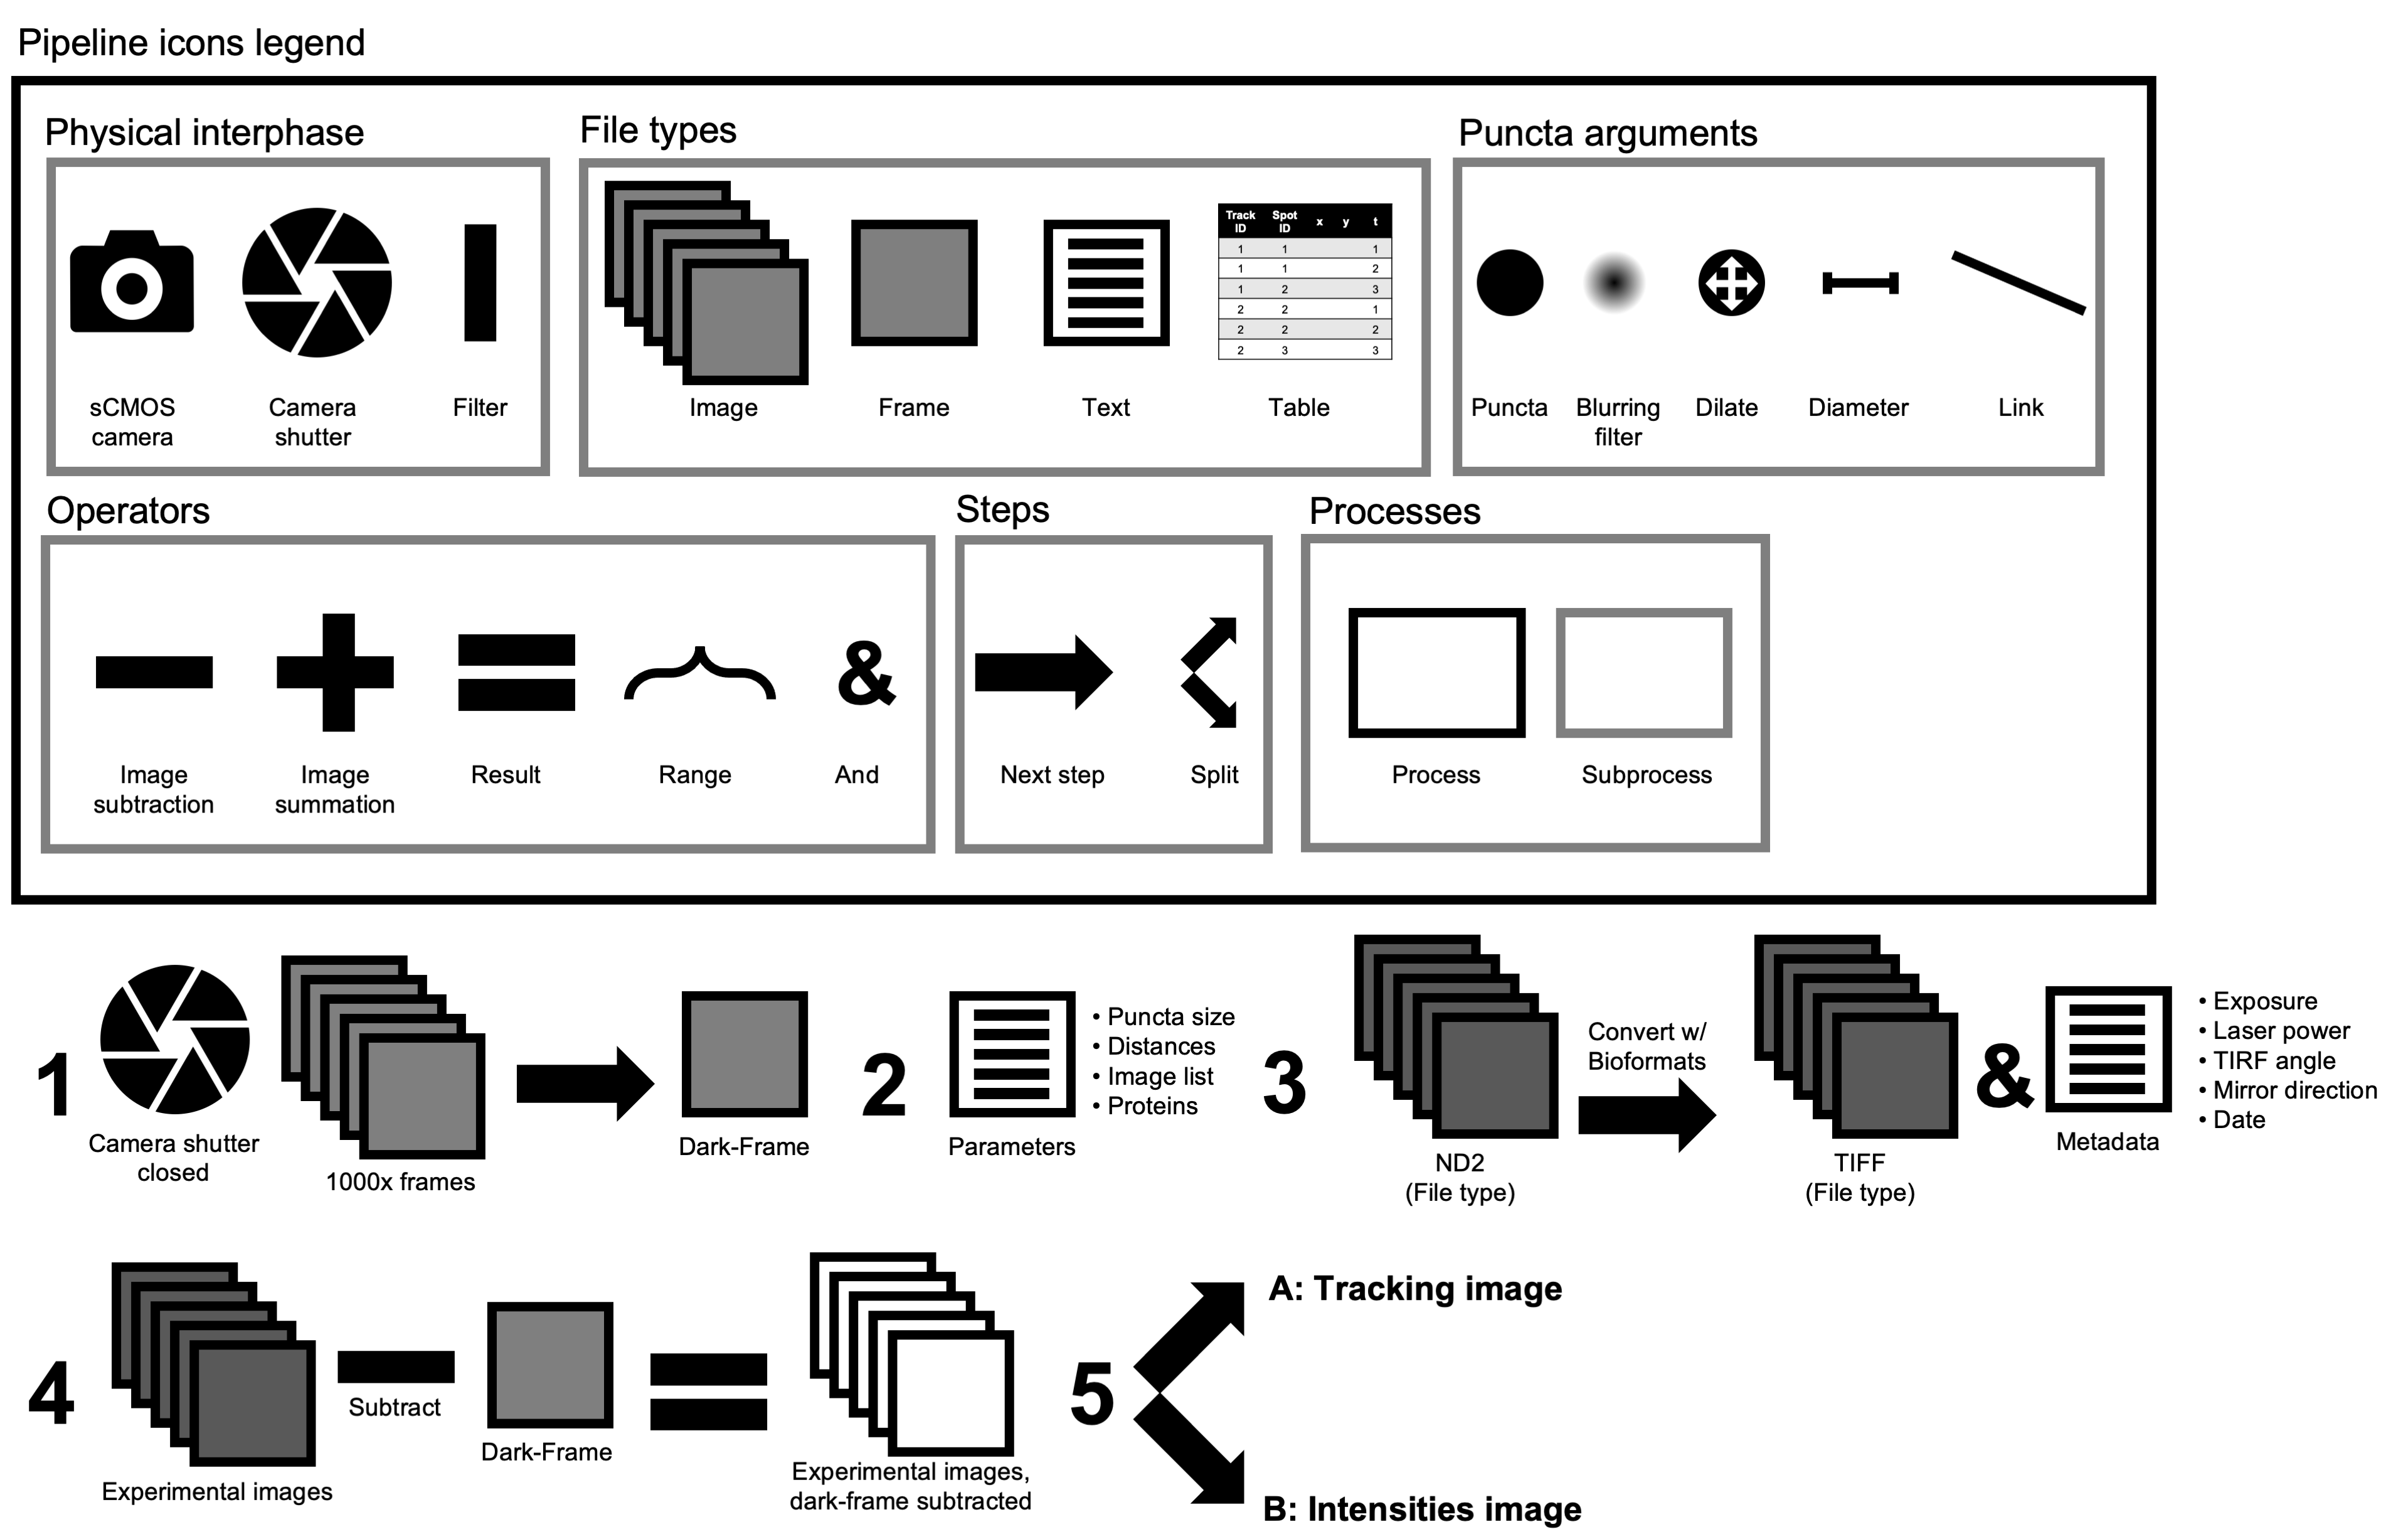
\includegraphics[height=\textwidth, width=\textheight, angle=-90, keepaspectratio]{methods/fig1.png}}
\captionsetup{parbox=none}
\captionof{figure}[Pipeline uses the metadata to remove the dark-frame]{\textbf{Pipeline uses the metadata to remove the dark-frame.} All icons used in this section are included in the pipeline legend.
\\
\\
(1) The pipeline starts with the determination of the dark-frame, which is the thermal noise in the camera. To calculate the dark-frame, the camera shutter is closed. Then, 1000 frames are acquired at the exposures used in the experiments.
\\
\\
(2) Input the parameters of the pipeline, including the image list, names of proteins in each channel, and the puncta size.
\\
\\
(3) The pipeline starts by converting proprietary formats to TIFF, the gold standard scientific image type. The pipeline saves the metadata. It then extracts useful image information that is needed for future steps. That is, it extracts input parameters so that the pipeline is autonomous, and the user does not have to interact with the pipeline.
\\
\\
(4) The dark-frame is subtracted from the experimental images. The pipeline used the image metadata to make the decision of which dark-frame to use.
\\
\\
(5) The pipeline splits into two processes: calculating the tracking image and the intensities image.}
\label{m:1}
\end{centering}

\subsection{The tracking image uses median subtraction, median blur and moving averages}
\subsectionmark{Tracking image}
To obtain the sharpest puncta, I estimated the background around the puncta (emerging, for example, from diffused light) using a median filter (Fig.~\ref{m:2}.5A). Median filters are a type of smoothing filter whose strength is edge preservation. Edge preservation is the ability to remove (blur out) noise while keeping a sharp edge, that is, keeping the silhouette. This contrasts with Gaussian filtering in that Gaussians blow-up the image features (in computer vision, features are information of image properties). For estimating the background around a puncta, I used a slightly dilated diameter from the puncta diameter used in particle tracking. I duplicated the puncta size. This would result in a 10-pixel diameter. Median filters extract all the values around a defined circle diameter, and sorts the values from smallest to largest, and then assigns the middle value to the center of the circle. The equation of a median is:
\begin{equation*}
\text{Median}(X) = 
\left\{\begin{array}{lr}
X[\frac{n+1}{2}], & \text{if }n \text{ is odd}\\
\frac{X[\frac{n}{2}]+X[\frac{n}{2}+1]}{2},& \text{if }n \text{ is even}
\end{array}\right.
\end{equation*} where $X$ is an ordered list of intensities and $n$ is the diameter of the median filter. If I use a 10-pixel size diameter ($n$), then there would be two middle values which are then settled by calculating the mean of the two center values. In other words, I would calculate the mean ($\mu$) for the two middle values ($n/2$ and $n/2+1$). This is an issue because if the data is non-parametric (for example, log distributed), then the mean ($\mu$) will be skewed. To employ a true median ($\frac{n+1}{2}$), I used a 11-pixel radius for estimating the background around a puncta (Fig.~\ref{m:2}.5A). The middle value would then be the 6th pixel intensity in the ranking. Lastly, I subtracted the median-blur image from the experimental images whose dark-frame was subtracted (Fig.~\ref{m:2}.5A). Calculating medians is computationally intensive which is why it is not employed as frequently as Gaussian blurs. It has to rank all pixels instead of summing them. There is a need to increase the speed of processing.

My previous pipeline did not make use of the full computing power available, running single-threaded in one central processing unit (CPU) only. For this second pipeline, I parallelized the scripts to make use of all the computer CPU resources available. Parallelization is a process which breaks tasks into smaller tasks and distributes them across processors. This approach enables using multiple processors for the job, and speeds up the analysis considerably as a result. More importantly, the scripts were rewritten so that it is compatible with cluster computers (high-performance computing also called “supercomputers”). For the cluster I used, Raven of the Max Planck Computing and Data Facility (Garching, Bavaria, Germany), I had 72 CPUs available. Theoretically, this means scripts now run 72\times faster. In principle, it could run faster using graphical processing units (GPUs), but this requires specific hardware which would make reproducibility more challenging.

The camera generates random fluctuations for each pixel, independent of the puncta fluorescence intensities \autocite{Diekmann_2022}. I used two methods to address this which can be thought of as time-independent and time-dependent in that the time independent uses only one frame and the time-dependent takes multiple observations taken at multiple times. Starting with the time-independent method, I applied a median blur of 3-pixels to even out the field (Fig.~\ref{m:2}.5A). Because puncta are 5-pixels in diameter and median filters are edge-preserving (keeps silhouette), a 3-pixel median-blur would still be able to show punctate structures while removing noise. However, the intensity measurements are now skewed, and random noise can appear punctate-like. To counteract this, I obtained intensity measurements from another image.

The second method for (“time-dependent”) random interference noise reduction that I used is called the moving average. In addition to counteracting random fluctuations emanating from the camera sensor, moving averages also help account for fluorophores blinking (flicker) \autocite{Dickson_1997}.

Moving average projections (image combination) work first by splitting the image into subsets of frames (k, also called the window) (Fig.~\ref{m:2}.5A). It then calculates the average of each pixel intensity at the same xy coordinate, and after, it creates a new list of average values which uses the xy coordinates to become an image. The frame is then shifted by one and the process is repeated again, that is, take the preceding and succeeding (original) frame, and calculate the mean. The other way to do this is a more familiar method which is called a group t-projection (group time combination). Group projection would average the three frames, and move three frames forward, and repeat the process again. The running average produces the same number of frames minus the window plus one while the group t-projection would divide the number of frames by the window size. For our window of three frames, say I have 99 frames in the original image, the running average that I use would produce 97 frames while the group t-projection would offer 33 frames. It is for this reason that I use the running average method.
\begin{equation*}
\text{SMA}_k = \frac{int_1 + int_2 + \cdots + int_k}{k}
\end{equation*}
Where $k$ is the window.

Running averages can potentially create an artifact known as motion blur (ghost-like image trails) which is an undesired consequence of the camera exposure. This effect emerges because camera exposure needs to be high enough to capture light, but not too high as to make it impossible to identify puncta. Motion blur arises in puncta that are traveling fast. For a single frame, this can be calculated as half the pixel length per exposure time.
\begin{equation*}
blur_{\text{tolerance}} = \frac{\text{pixel size}}{2}\times \text{exposure}
\end{equation*}

Our camera has a resolution of 0.147 µm/pixel, thus motion blur would emerge for puncta traveling faster than 0.37µm/s for a 200 ms exposure, or 1.46 µm/s for a 50 ms exposure. This is the tolerance (parametric limit) for the intensity reference image. However, because I are using a running average with a window of three frames (or 12 seconds since I used 0.25 frames per second), our objects would need to move between 0.03 to 0.12 µm/s for exposures at 50 and 200 ms, respectively, to be tracked appropriately.
\begin{equation*}
blur_{\text{tolerance}} = (\frac{\text{pixel size}}{2}\times \text{exposure}) \times (k \times \text{frame rate})
\end{equation*}
where $k$ is the window.

The easiest way to offset the effects of motion blur would be to use a small window, which in my case, I used three frames (it is an odd number so that values can be centered; say I have three frames, it would use the time of the second frame as the new timestamp) (Fig.~\ref{m:2}.5A).

Motion blur can create long tails that seem like comets. Another way to remove the effects of motion blur lies in the rigid 5-pixel diameter of the puncta that TrackMate uses in detection. TrackMate detects puncta by fitting 2D-Gaussian curves (normal curves in xy axis) (Fig.~\ref{m:4}.7A), then calculates the derivative (change between pixel before and after) of the fit, and after, applies a Laplacian operator (second derivative, that is, the change of change) to find edges (boundaries). The result is then inverted, and TrackMate then centers the puncta around the local maxima (relative brightest value) (Fig.~\ref{m:4}.7A). Thus in a perfect world, an image moving linearly whose intensity remains constant would have the correct puncta centroid. However, puncta moving randomly (like Brownian motion) would have a less accurate centroid. For my system, MyD88 is likely traveling via the cytoskeleton, which means movement is predictable. However, if the intensity fluctuates, TrackMate could potentially use the wrong centroid. This is another reason why I use the intensity reference image, to counteract this.

Another artifact motion blur can introduce is overcorrection. Puncta that persist only for one frame would be dimmer than the original intensity (if using the mean as it would average two dim values and one bright value), or disappear (if using median as the center value of two dim and one bright event would be a dim event). However, distinguishing noise from puncta would be difficult, and our script requires a minimum dwell time (persistence) of three frames in order for puncta to be included in the analysis. Another artifact that could be introduced is having “shadow” intensities in the preceding and succeeding frames. While this can be an artifact, it can also be advantageous in that it can boost intensities of dim puncta, and allows us to measure the beginning and the end of the puncta better. Moreover, I obtained intensities from a different image. At worst, the intensity would read close to zero, which means it can be addressed in the post-processing of the images as I have an intensity reference image.


\begin{centering}
\centering{\includegraphics[height=\textwidth, width=\textheight, angle=-90, keepaspectratio]{methods/figS2.png}}
\captionsetup{parbox=none}
\captionof{figure}[The tracking image offers high signal-to-noise at the expense of skewing intensities]{\textbf{The tracking image offers high signal-to-noise at the expense of intensities.} The tracking image is highly processed so that high signal low background can be achieved. However, this comes at the expense of the intensity values which are now considerably lower than the dark-frame removed image. The tracking image starts with the estimation of the background around the puncta using a median (edge-preserving) filter of size 11-pixels (2\times puncta size + 1 to make it odd, that is, a true median). Then, the blur is subtracted from the dark-frame removed image. This results in an image with low cytosol noise. Yet, there is considerable noise due to random intensity fluctuations. To remove this source of noise, I took two approaches, one time independent and another time dependent. The time independent method uses median blurs of a diameter slightly smaller than the puncta. In this case, it is 3-pixels. The resulting blurred image is then passed through a moving average filter, so that random fluctuations can be removed in a time dependent manner. I took three frames, and averaged the intensities, pixel by pixel (xy coordinate). Then, the resulting mean image is saved. This process is done iteratively, shifting by one frame. The resulting image is then summed with all other channels (the reference plus the query proteins). The output of this I call the tracking image.}
\label{m:S2}
\end{centering}

\begin{equation*}
\text{tracking image = }\sum_{i = 1}^{c}\text{dark-frame removed image}_i
\end{equation*}

Proteins are labeled with fluorophores so that they can be selectively visualized with fluorescence microscopy. This is the principle of fluorescence microscopy. For fluorophores to be seen, they need to be excited (illuminated) with a particular wavelength (Fig.~\ref{m:2}.5). Then, they emit (bounce) at another specific wavelength (Fig.~\ref{m:2}.5). In the case of green fluorescent protein (GFP), the excitation is cyan light and the emission is green light (Fig.~\ref{m:2}.5). Cells can reflect the excitation light. To only see the light in the expected emission spectrum, a filter is used to block the excitation light out and let the emission light pass (Fig.~\ref{m:2}.5). My camera is monochromatic. This means I can use a single camera to visualize two fluorophores to see two proteins.

To see the different proteins we labeled, we had to capture two images, one at each color channel (eGFP, mScarlet) (Fig.~\ref{m:2}.5). I observed punctate structures. Software can track puncta over time. To be able to determine if the different proteins are colocalized, there are two approaches to calculate puncta colocalization: tracking puncta separately or together.

In the previous chapter, I used to track puncta in different channels separately. I used a script to pair puncta in different channels using the distance from its coordinates, and measured how long did these puncta in different channels (proteins) dwell together (called the dwell time). From this, the script then decided which puncta belong together. One issue I had was that it became difficult to distinguish which puncta belongs to who. The cells had several puncta. This meant that sometimes, the script assigned one “reference” protein to several “query” proteins. To make things harder, Myddosome puncta are highly dynamic, continuously splitting and merging. This means a puncta can start with one query puncta that then splits off (completely or partially, both are possible), or puncta merge. To address this issue, the new pipeline combines the different channel images into one (Fig.~\ref{m:2}.5A). Now, the decision of which puncta are colocalized rests on the particle tracking software that I used, TrackMate.

With all this in mind, I have now created a tracking image for TrackMate. Later, I will need to fix the timestamp so that it uses the center frame value (Fig.~\ref{m:S2}.5A).

\subsection{The intensity image uses median subtraction to remove cytosolic background}
\subsectionmark{Intensity image}
For the intensity image, I first used the dark-frame subtracted images. Then, I median-blurred these images using a 3.7 µm (25-pixel) diameter, about half the cell diameter (Fig. Fig.~\ref{m:S3}.5B,~\ref{m:2}.5B). The resulting image is an estimate of the cytosol fluorescence (background). After, I subtracted the median blur from the dark-frame removed images (Fig. Fig.~\ref{m:S3}.5B,~\ref{m:2}.5B). The resulting image is the intensities reference image (Fig.~\ref{m:2}.5B). This image was used to obtain intensity measurements from the puncta (Fig.~\ref{m:S3}.5B).

Up to this point, the pipeline has saved four images: the original image, the dark-frame removed image, the tracking image, and the intensities reference image. To calculate the signal-to-noise ratio, I took a sample puncta of 5-pixels in diameter as a signal measurement, and a box outside the cell for my background measurement. From these regions, I calculated the mean intensity and then divided the signal by the background to obtain the signal-to-noise ratio (SNR). The original image had a lot of background. The SNR was two. The dark-frame removed image had most of the camera background eliminated, and had a SNR of seven. After, the intensities reference image whose cytosolic estimate was removed, had a SNR of 31. Lastly, the tracking image had the best SNR, at 40. However, the signal was 73\% dimmer than the dark-frame removed image (Fig.~\ref{m:S3}.SN). By comparison, the intensities reference image was 35\% dimmer than the dark-frame removed signal.


\begin{centering}
\centering{\includegraphics[height=\textwidth, width=\textheight, angle=-90, keepaspectratio]{methods/figS3.png}}
\captionsetup{parbox=none}
\captionof{figure}[Another image set is generated with intensities preserved but cytosol fluorescence removed]{\textbf{Another image set is generated with intensities preserved but cytosol fluorescence removed.} Different images were created with different purposes.
\\
\\
(5B) The intensity reference image is generated so that I have accurate intensity readings. To accomplish this, I first estimate the cytosolic background using a median blur whose diameter is half of that of a cell, about 25-pixels. Then, this background estimate is subtracted from the dark-frame removed image. The resulting image is the intensity reference image. (Signal-to-Noise) To illustrate the advantages of my pipeline, I took a sample puncta and calculated its mean brightness (signal) and then divided it by a region with no cells (the background). The quotient is called the signal-to-noise ratio (SNR). The original image has poor SNR. After removing the dark-frame, there is improvement, but the true improvement happens after processing the image. The intensities reference image has a SNR of 31 which also preserves the signal strength. The tracking image has a SNR of 40 which is great for tracking, but not for measuring intensities. It is for this reason that multiple images were created by this pipeline.}
\label{m:S3}
\end{centering}


\begin{centering}
\centering{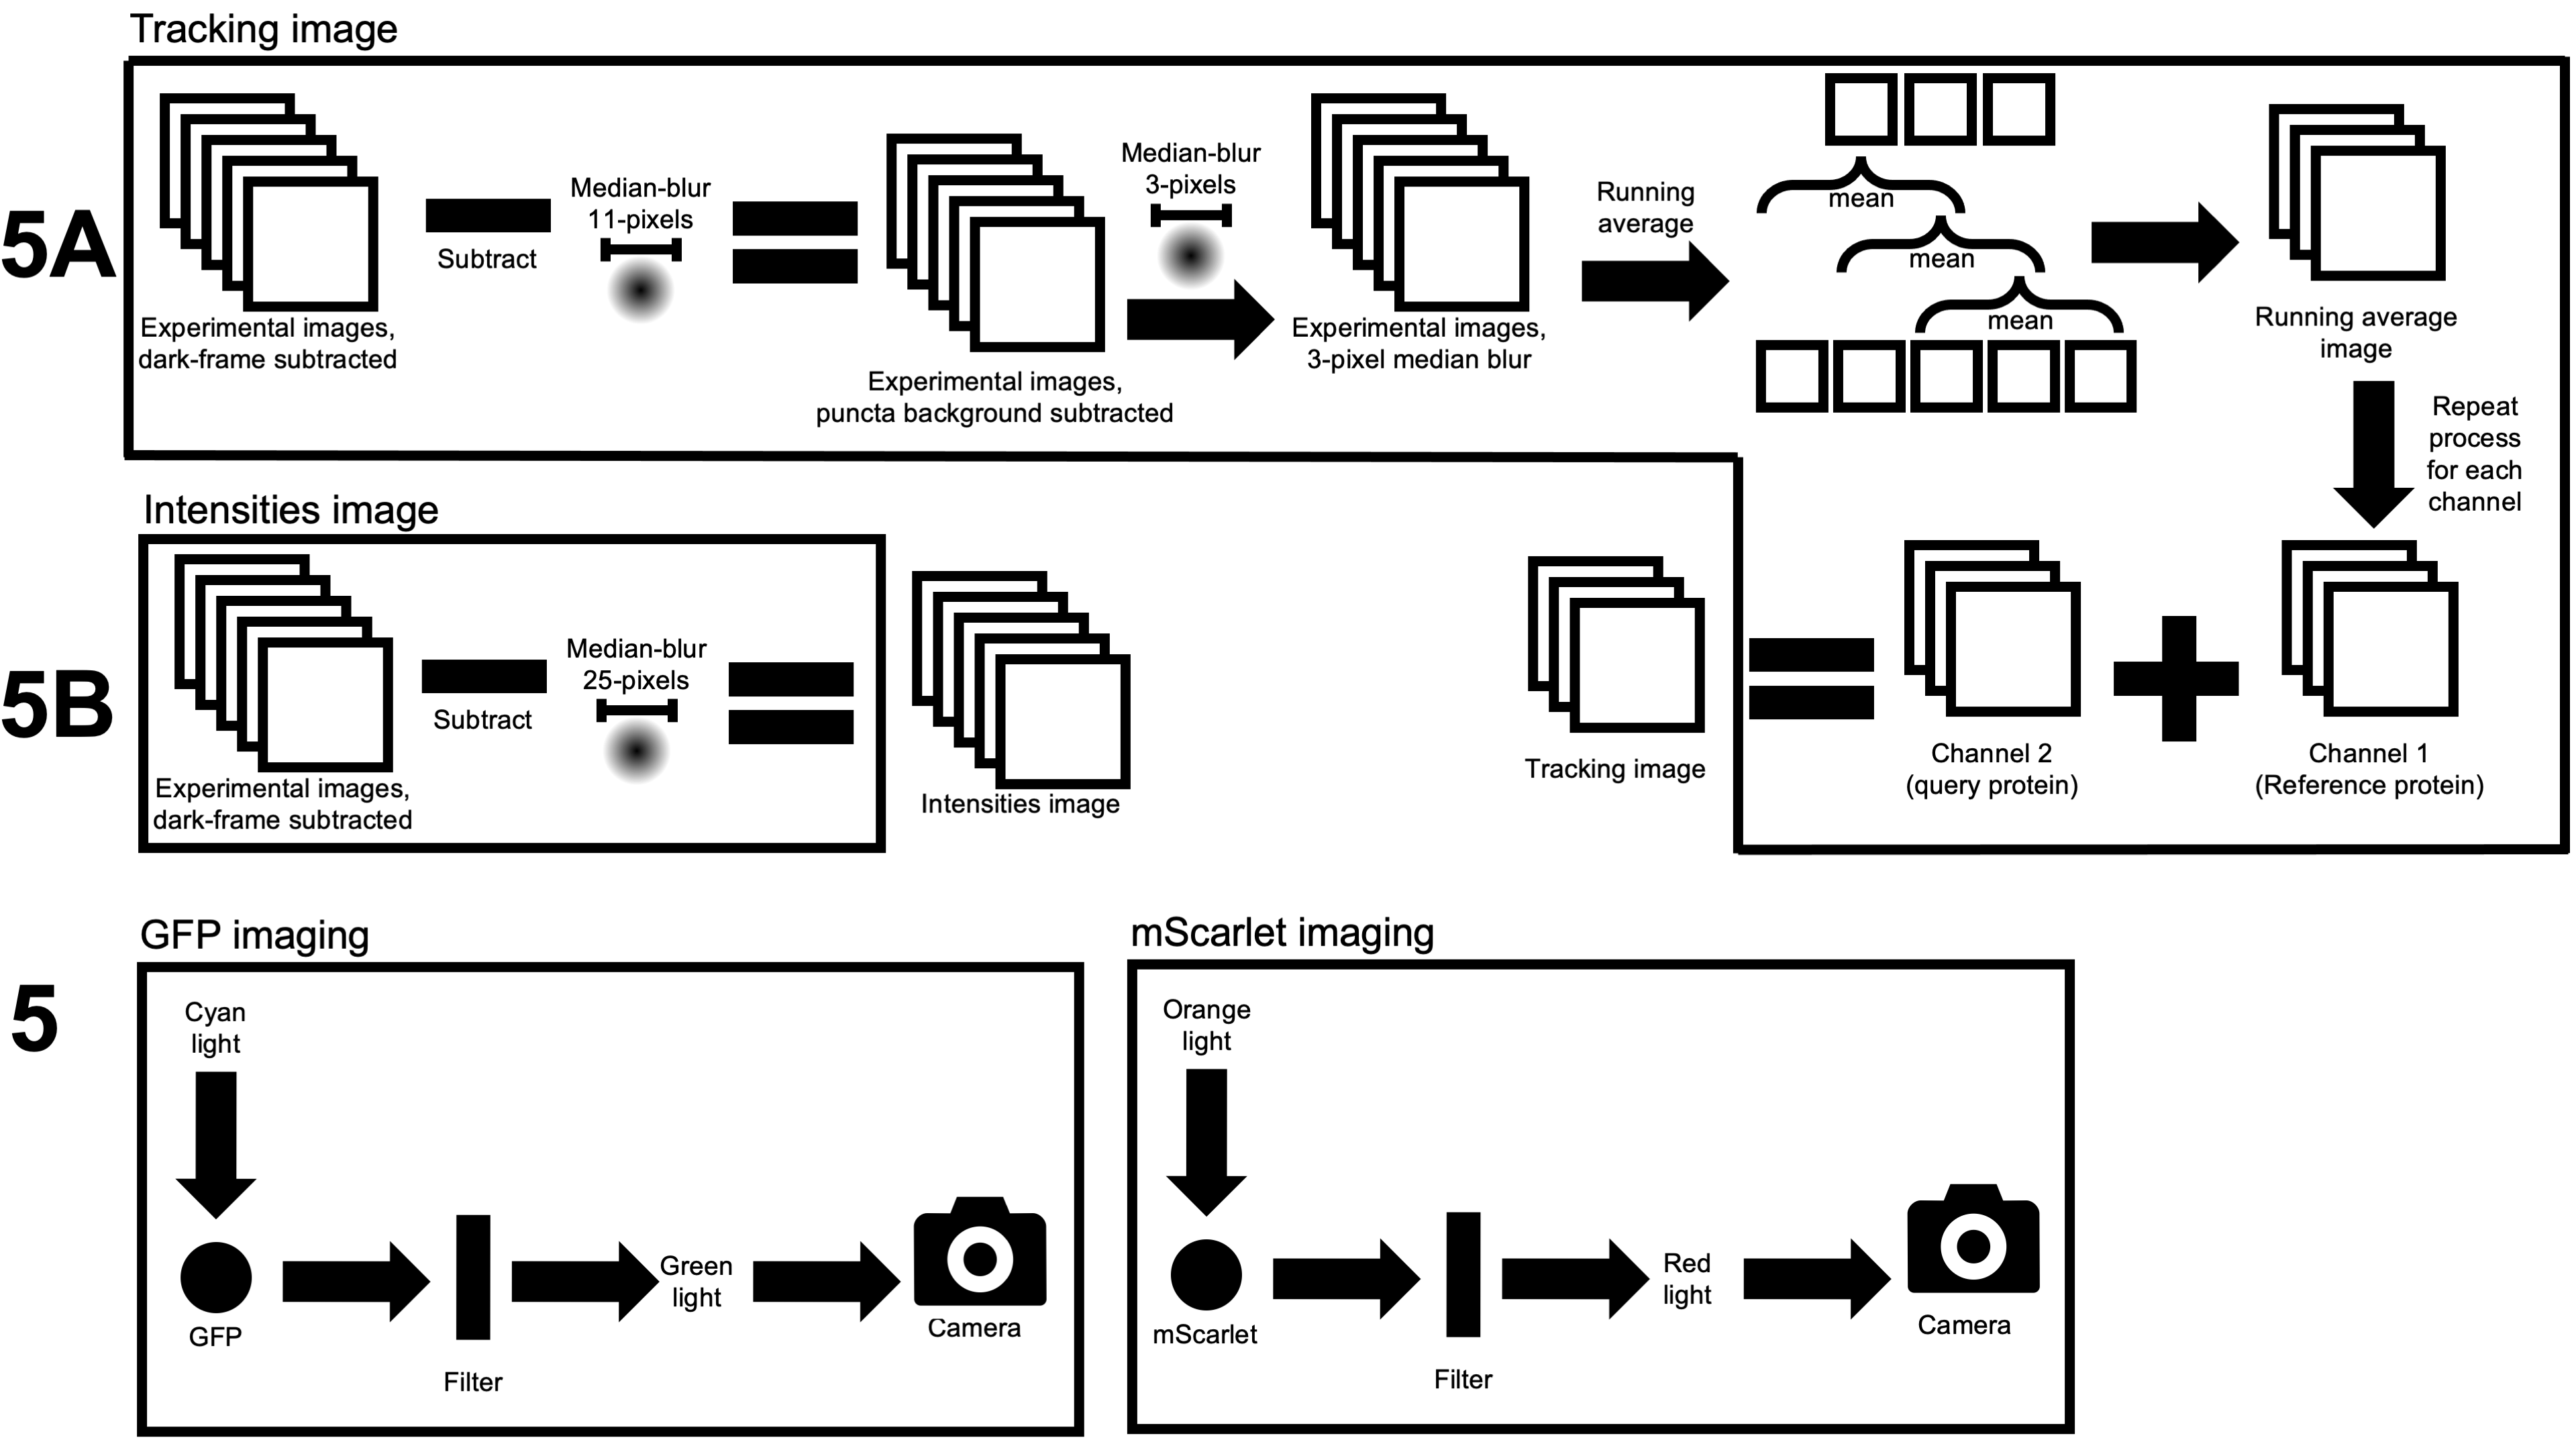
\includegraphics[height=\textwidth, width=\textheight, angle=-90, keepaspectratio]{methods/fig2.png}}
\captionsetup{parbox=none}
\captionof{figure}[The tracking and intensity-measurement images are created fit for their purpose]{\textbf{The tracking and intensity-measurement images are created fit for their purpose.}
\\
\\
(5A) The tracking image process begins with the subtraction of the puncta background. This is accomplished by calculating a median blur twice as large as the puncta (plus one if this number is even, so that it uses a true median and not an average). Then, it subtracts the blurred image from the experimental image. After, a median blur of 3-pixels in diameter (slightly smaller than the puncta) is applied so that random fluctuations of the camera sensor are removed. Lastly, also for removing random fluctuations, a running average is calculated.
\\
\\
(5B) The intensity-measurement image estimates the cell cytosolic background using half of the cell diameter, that is, 25-pixel in diameter. It then subtracts this blur from the dark-frame removed experimental image.
\\
\\
(5) Diagram showing the microscope setup. Fluorophores are excited with laser light, then a filter blocks out unwanted light that falls outside the expected color. Lastly, the expected light is collected by the sCMOS camera sensor.}
\label{m:2}
\end{centering}

\subsection{Cell segmentation speeds-up the analysis, and enables identifying biological replicates}
\subsectionmark{Segmentation}
The images we captured can potentially fit well over forty cells. If I quantify whole images as-is, then cell-specific information is lost. In image processing, one method for identifying cells in images is called segmentation. Segmentation is a technique which partitions (breaks-apart) images into smaller parts (segments). It uses the features (characteristics) of the image to identify the boundary.

Studies have typically used cytosol and nuclear staining to identify where cells are located. However, traditional staining is often toxic to the cell, which is incompatible with my goal to quantify live cells. The staining can also interfere with the fluorophores, reducing the number of colors I have at my disposal. Therefore, I had to take a different approach to segmentation. In my case, I used the fluorophores to identify where cells are. The advantage of MyD88 is that it is distributed throughout the cytoplasm which offers a cell outline, and it aggregates into “super-myddosome” centers which can be used as markers of cells. I exploited these properties of MyD88 for my segmentation pipeline.

The first step I took towards segmentation was to identify how many cells there are, and where their centroids are. I found the maximum brightness value at each pixel position using the intensities reference image (Fig.~\ref{m:3}.6A). This method is termed max projection. Projection means the combination of images per pixel coordinate (position). Then, I adjusted the contrast so that the full range of intensities can be seen. In theory, this contrast adjustment is achieved by rescaling the image intensities, setting the dimmest intensities to zero and the brightest intensities to one and then multiplying it by the bit rate of the TIFF image.
 \begin{equation*}
int_\text{scaled} = \frac{int - \text{min}(int)}{\text{max}(int)- \text{min}(int)}
\end{equation*}
Where $int$ is the intensity.

In practice, the rescaling max value can be set not only to the max (like in this step) but also for quantiles (as I do later in this pipeline). The bit rate is the range of values allowed. Because computers use binaries (0, 1), the bit depth would be the bit length (how many positions one has to put 0 or 1, for example 000 would be 3-bits) to the power of two minus one so that intensities can start at zero. A diagram of how this works is available at Fig.~\ref{m:3}.Binary numbers.

The most common TIFF bit depths used in science are 8-bit (255 levels) and 16-bit (65,536 levels). For our 16-bit camera, the values were scaled from 0 to 65,536. The resulting image is called the marker because it marks where the cells are.

I calculated the cell centroid marker (“marker”) using the brightest MyD88 region (Fig.~\ref{m:S4}.6A,~\ref{m:3}.6A). To accomplish this, I first calculated what is the maximum intensity (brightness) achieved on each pixel (Fig.~\ref{m:S4}.6A,~\ref{m:3}.6A). Then, I created two images from this max projection: Gaussian and median blur images (Fig.~\ref{m:S4}.6A,~\ref{m:3}.high-pass filter). The Gaussian blur was used to obtain a cytosol estimate. I used a diameter of 15-pixels (three times larger than that of a puncta) (Fig.~\ref{m:S4}.6A,~\ref{m:3}.high-pass filter). Then, for the median blur, I used the same diameter as the puncta (Fig.~\ref{m:S4}.6A,~\ref{m:3}.high-pass filter). This way, the subtraction of the Gaussian from the median shows the brightest puncta (Fig.~\ref{m:S4}.6A). After said subtraction was performed, the difference was log transformed (Fig.~\ref{m:S4}.6A,~\ref{m:3}.high-pass filter). This transformation was used because the MyD88 puncta intensities show a wide range of intensities which are log-distributed. Therefore, a log-transformation would make the puncta intensities more uniform (Fig.~\ref{m:S4}.6A). After, I applied a median blur of 3-pixels (slightly smaller than the puncta) (Fig.~\ref{m:3}.high-pass filter). This was done so that the puncta are clearer (Fig.~\ref{m:S4}.6A). Lastly, the image was thresholded using connected components labeling. Connected components labeling is an application of graph theory which is commonly used for identifying blobs. It looks at neighboring pixels and decides if the intensities are similar or different. After, the image was made into a binary (Fig.~\ref{m:S4}.6A,~\ref{m:3}.6A).

I calculated what is called the mask which in this case is the cell edges (boundaries). I took all the frames and calculated the mean average intensity per pixel position (xy-coordinate) (Fig.~\ref{m:3}.6B). I adjusted the contrast like I did in the marker. I proceeded to identify where the cell edges are using the difference of two blurs. Specifically, I calculated a Gaussian blur of 15-pixels of the cells because this would dilate (blow-up in size) the brightness of the puncta (Fig.~\ref{m:3}.6B). This makes the dim regions of the cell brighter at the expense of making bright regions dim. Then, I applied a median filter of 5-pixels, the same as the puncta, so that I can identify the brightest regions. I then subtracted the median from the Gaussian image. This leaves me with only the brightest puncta (Fig.~\ref{m:3}).


\begin{centering}
\bigfig{\centering{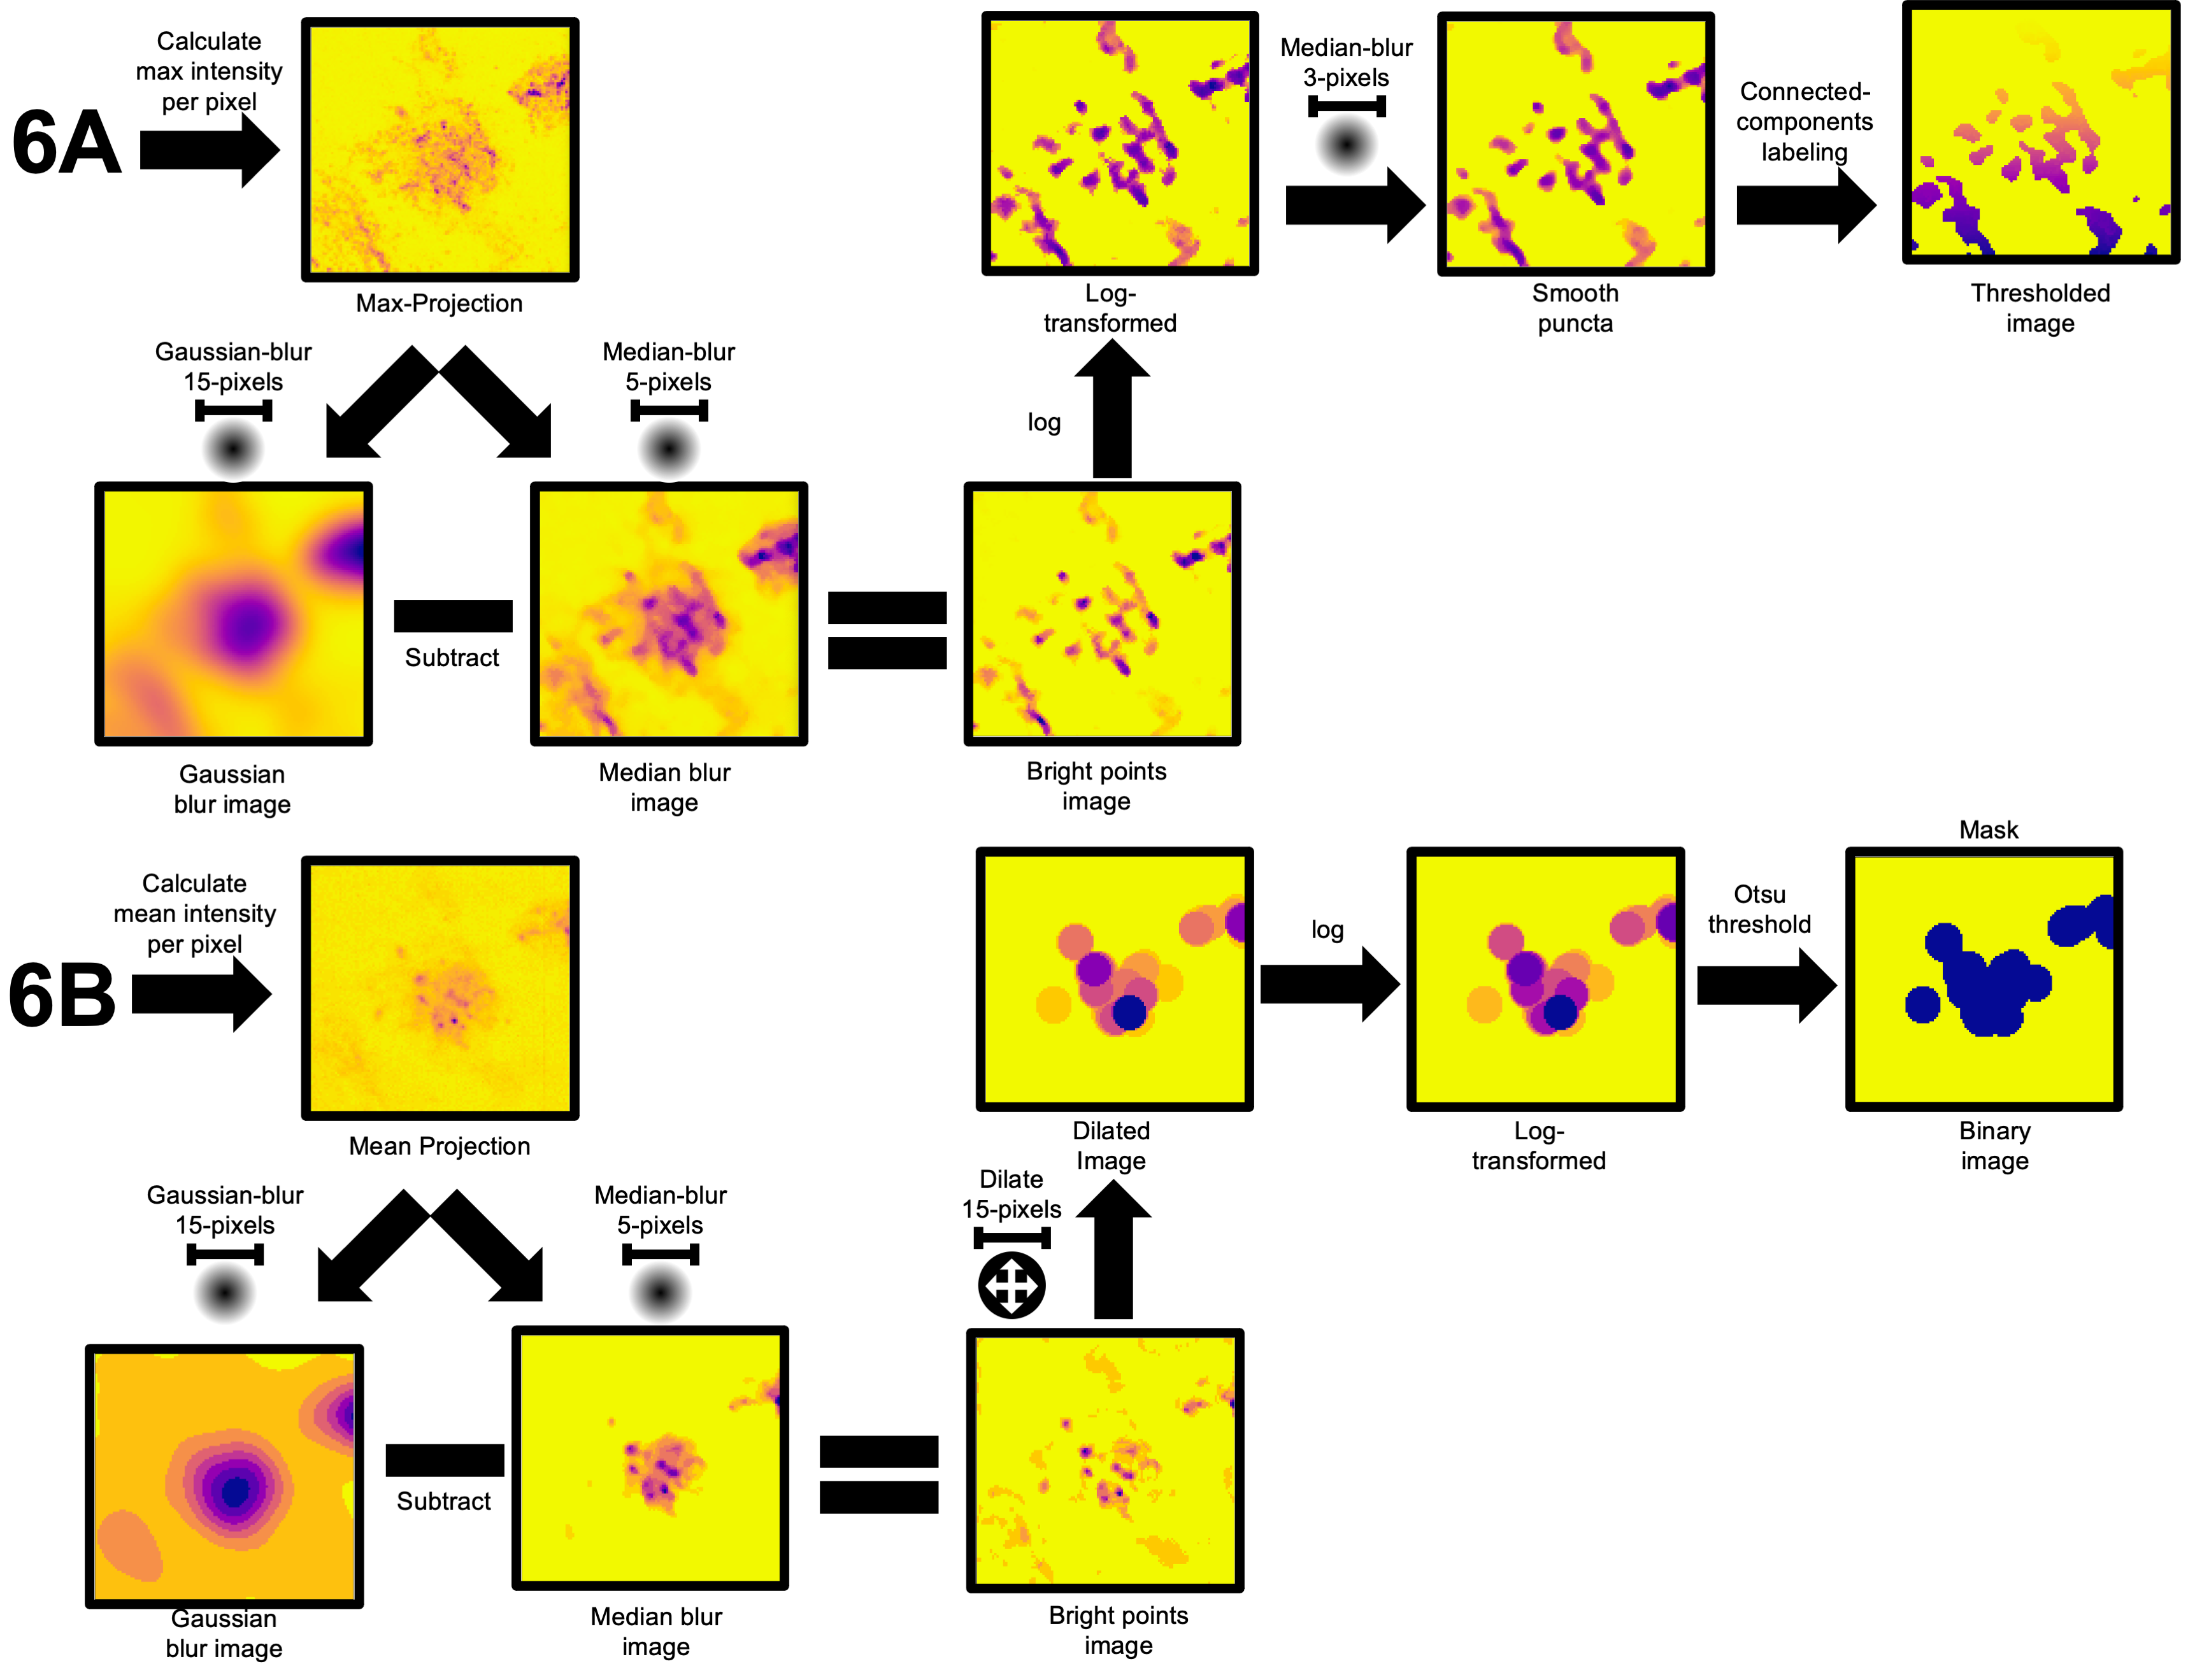
\includegraphics[height=\textwidth, width=\textheight, angle=-90, keepaspectratio]{methods/figS4.png}}}
\captionsetup{parbox=none}
\captionof{figure}[Process for identifying the cell boundary]{\textbf{Process for identifying the cell boundary.} To segment cells present in the image, I used marker-controlled watershed segmentation. One of the requirements of this algorithm is to create a mask that outlines the cell boundary, and a marker that indicates how many cells there are present in the image.
\\
\\
(6A) Starting with the marker, I began by taking the maximum brightness of each pixel. I then duplicated this image, one having a Gaussian blur to estimate a dilated (blow-up) background, and the other had a median blur for estimating the location of puncta. I subtracted the Gaussian from the median image. This resulted in the “bright points image” where puncta are really clear. Because of the wide range in intensities, I log-transformed the image so that the difference between bright and dim points is linear, and not exponential. Then, I smoothed this image using a median blur. This image was thresholded using connected-components labeling. The final image is the marker.
\\
\\
(6B) The mask was estimated using a mean-projection image, that is, the mean intensity of each pixel. Again, I took the Gaussian to estimate the background, and subtracted it from the median blurred image. The resulting image offered sharp puncta. I then dilated these so that all puncta are included within the cell boundary. I log-transformed this image, and thresholded it using Otsu. This is the mask, the cell boundary}
\label{m:S4}
\end{centering}

The next step for segmentation is applying an algorithm called marker-controlled watershed segmentation. To understand how this algorithm works, we need to first examine watershed segmentation

It is called watershed segmentation because it uses the same principle as geographic watershed drainage basins. Therefore, I will first explain geography to better understand image analysis. A watershed is the land that collects water. The drainage basin is where this water flows to, typically rivers though it then makes its way to lakes and ocean. The water is driven to the drainage basin through gravity and elevation. It flows from the highest places (hills) down to the low regions (valleys).

For image analysis, the watershed is calculated using the mask as described above. The distance from the edge (background) needs to be determined. The further away from the background (cell edge), the higher the intensity. This would appear as a hill in an xy-plot (Fig.~\ref{m:S5}.Comparison). Between peaks, one can have valleys. In other words, the algorithm calculates the centroid of the binary (thresholded black \& white image) silhouette and treats it as a hill. Then, the further a pixel is from the parent hill, the lower the intensity “elevation.” This distance depression is treated as a valley (Fig.~\ref{m:S5}.Comparison). The algorithm then floods the image landscape, which explains why it is called watershed segmentation. The local minima between two centroids (hills) then becomes the boundary (the place where the river flows). However, the output is not perfect at identifying the valleys (Fig.~\ref{m:S5}.Comparison).

The marker-controlled watershed is an offshoot of the watershed segmentation. Here, the difference is that the marker (as described above) assists in the identification of hills, that is, the identification of foreground. If there are multiple markers, then more breaks are applied (more regions are identified), and if there is no marker, then there is no boundary. The resulting image is shown in Fig.~\ref{m:S5}.6C and how the algorithms compare is shown in Fig.~\ref{m:S5}.Comparison.


\begin{centering}
\bigfig{\centering{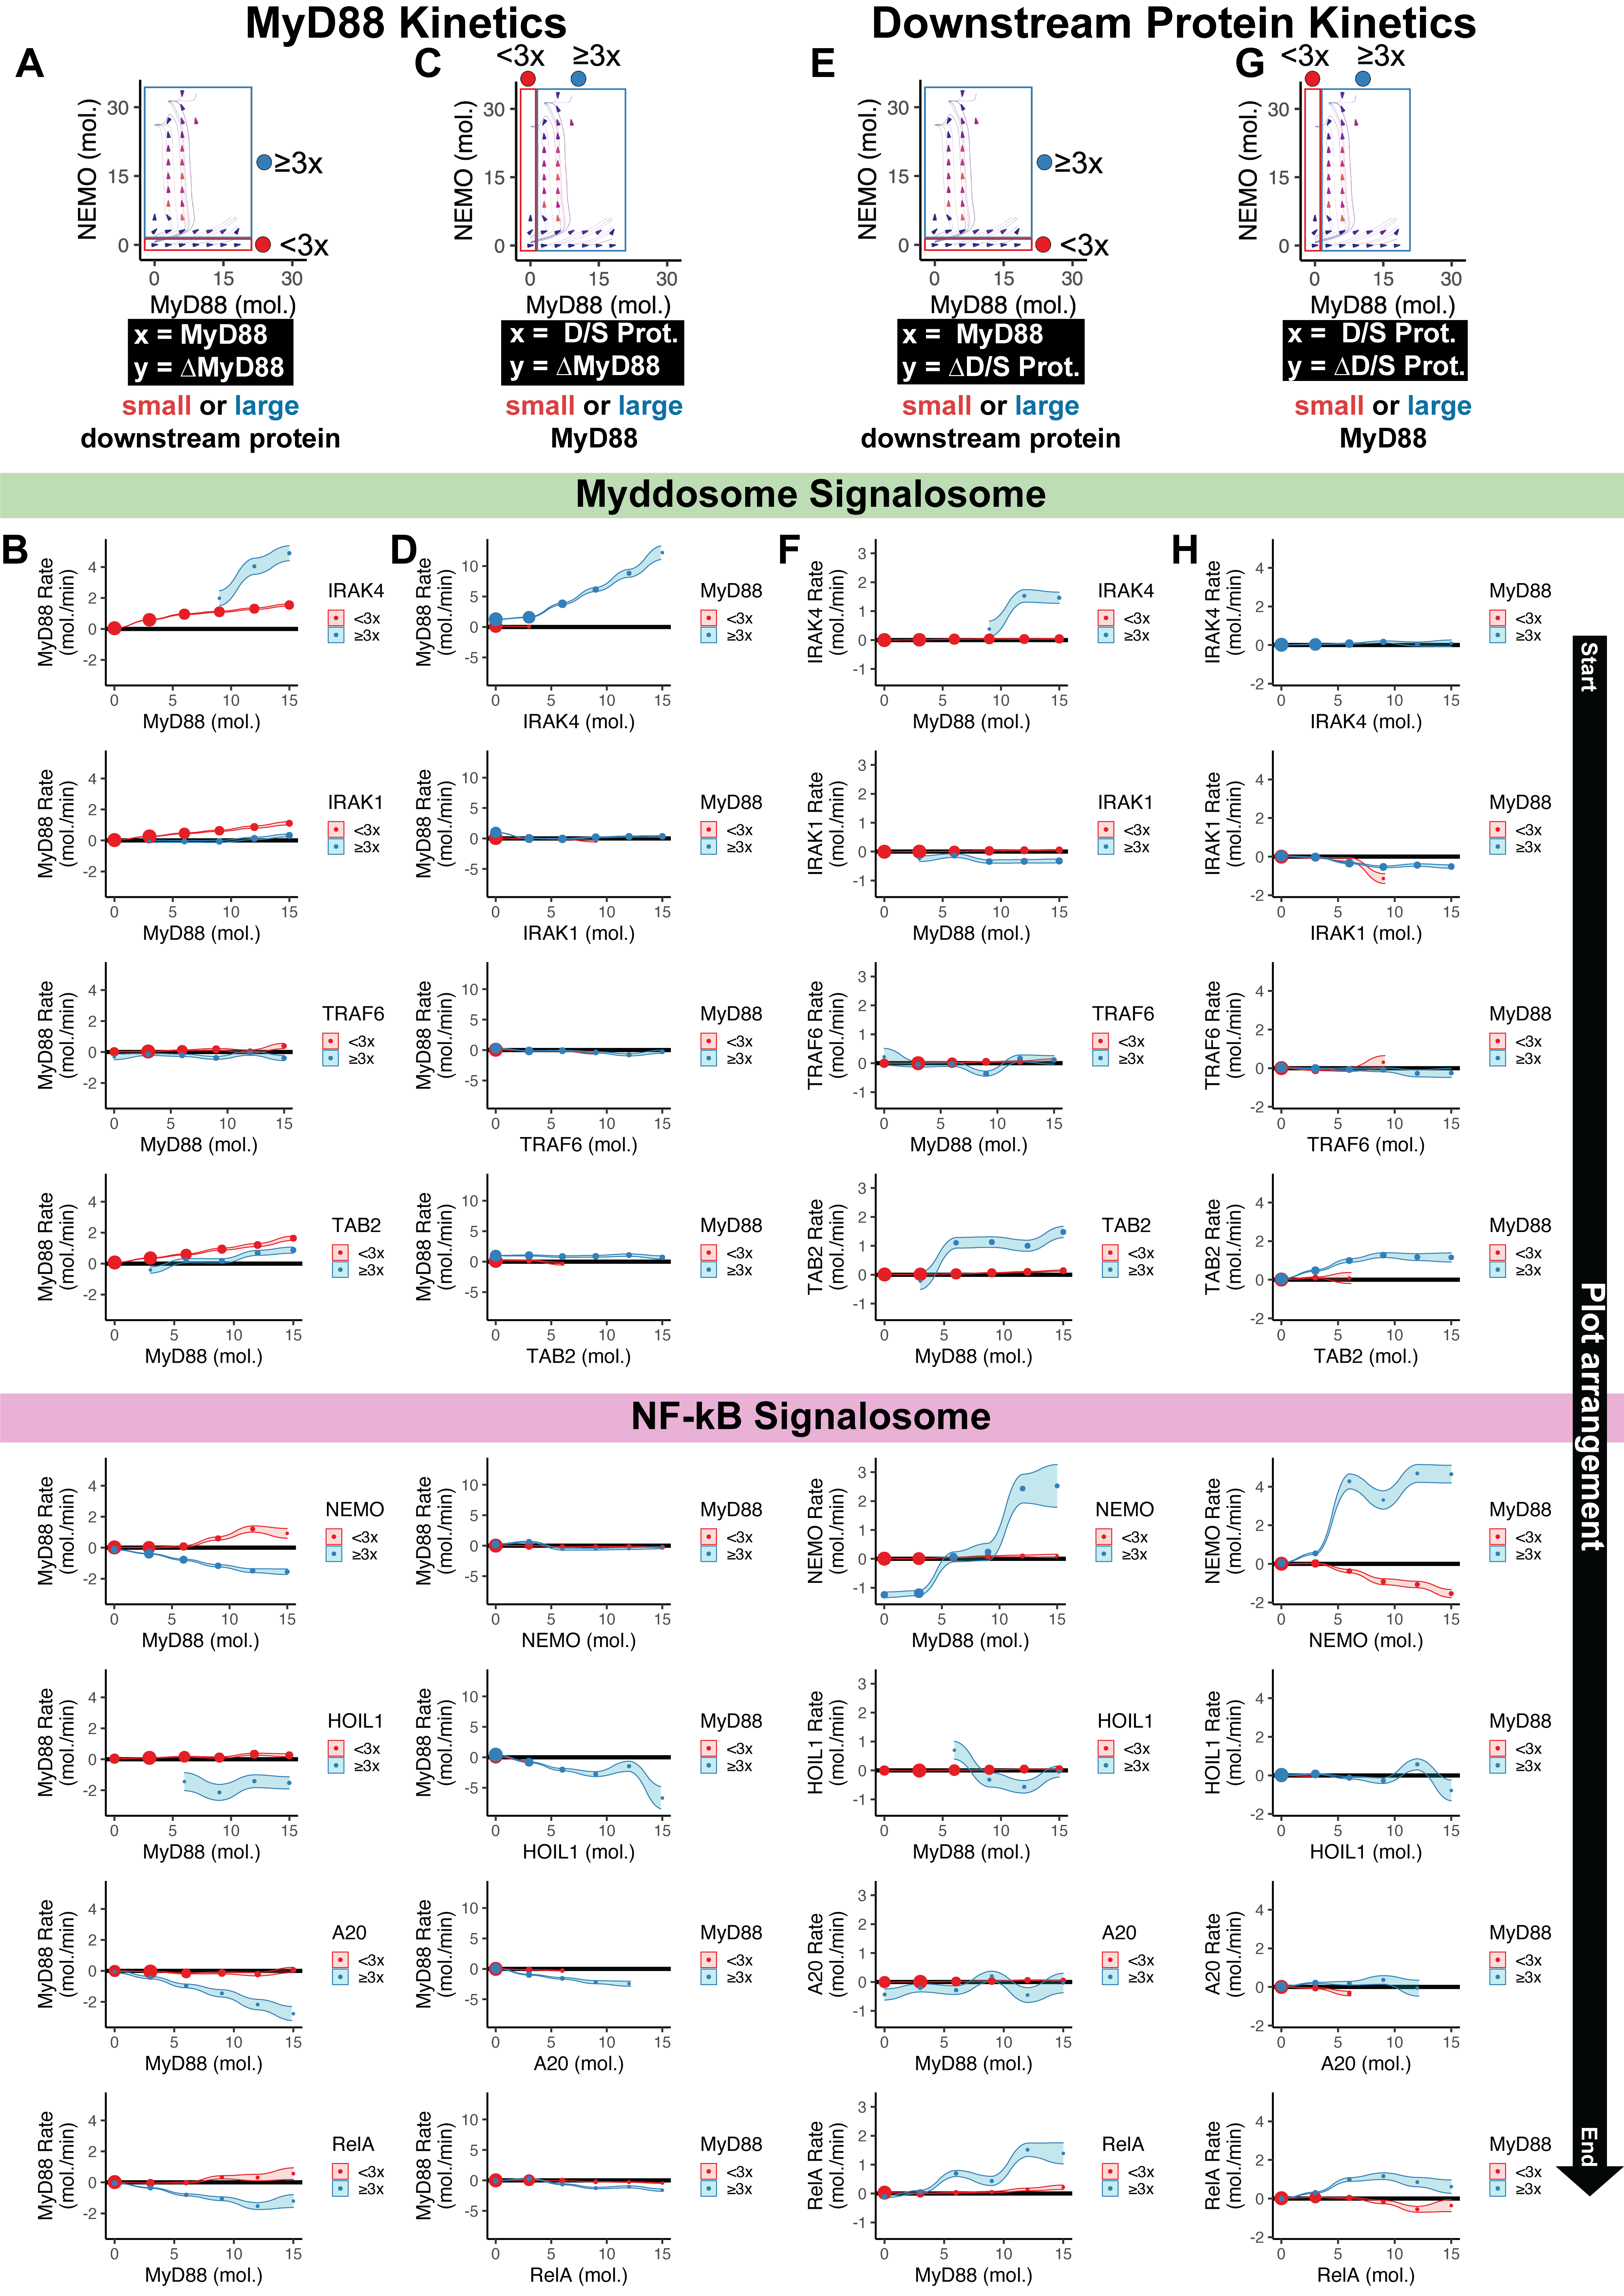
\includegraphics[height=\textwidth, width=\textheight, angle=-90, keepaspectratio]{methods/figS5.png}}}
\captionsetup{parbox=none}
\captionof{figure}[Identifying individual cells with marker-controlled watershed segmentation for measuring biological replicates]{\textbf{Identifying individual cells with marker-controlled watershed segmentation for measuring biological replicates.}
\\
\\
(Thresholded images) Before segmentation can take place, images need to be in binary format. Two images are required for marker-controlled watershed segmentation: the marker and the mask.
\\
\\
(Thresholded images, marker) The marker identifies where cells are, while the mask indicates the cell outline. Once these two are generated as described before, then watershed segmentation can be used. Watershed segmentation is based on geography. Watersheds are lands where water gets collected. The water then flows up from the hills down into the valleys using gravity. Rivers, lakes and oceans emerge at the drainage basins. This is illustrated on the top right corner.
\\
\\
(Photo) To show how geography informs the watershed segmentation algorithm, I used Lake Lucerne (Switzerland) as an example. For this example, Lake Lucerne is the drainage basin with Bürgenstock (mountain) marked as hills, and the towns of Stansstad and Rotzloch identified as the valley. The black line is to illustrate how watershed segmentation could segment this image.
\\
\\
(Distance maps) With that in mind, the first step for using this algorithm lies in calculating the distances from the cell silhouette (mask) edge. This is termed the distance map and is illustrated above. The most distant places to the cell boundary are treated as hills. Think of them as snow-capped mountains. Then, the depression between two hills (local minima) are treated as valleys. Like glaciers melting, the algorithm then floods the valleys. Wherever rivers emerge is the new cell boundary. For our sample image, classical watershed segmentation is indicated in the middle. However, my script uses marker-controlled watershed segmentation. “Marker-controlled” means that a marker image is used to help find the hills. In my analysis, the marker are the brightest regions (process described above). For the sample image, there are five blobs in the marker image. That means there should be five cells.
\\
\\
(Intensity images) When combined with the distance map, the cell boundaries are more accurately identified, as illustrated on the images.
\\
\\
(Comparison) The rightmost plot is a line profile. The color in the distance maps row of images indicates the distance from the edge. For the line plot, that became the y-axis. The black line in the image is the x-axis, with the origin on the left. The vertical lines in the plot are for indicating where the classical and marker-controlled watershed segmentation algorithms identified cell boundaries. Notice how the marker-controlled watershed segmentation is superior at identifying the hills and the valleys.
\\
\\
The distance maps (bottom row) were drawn for the marker, mask (only for completeness) and with each segmentation algorithm. Then, these were converted into 3D surface plots using the distance from the mask edge. The custom color palette (white-brown-blue) was only to simulate snow-capped mountains and lakes.
\\
\\
(6C) Marker-controlled watershed segmentation of the cells illustrated in figure~\ref{m:S4}.
\\
\\
Photo captured by the thesis author.}
\label{m:S5}
\end{centering}


\begin{centering}
\bigfig{\centering{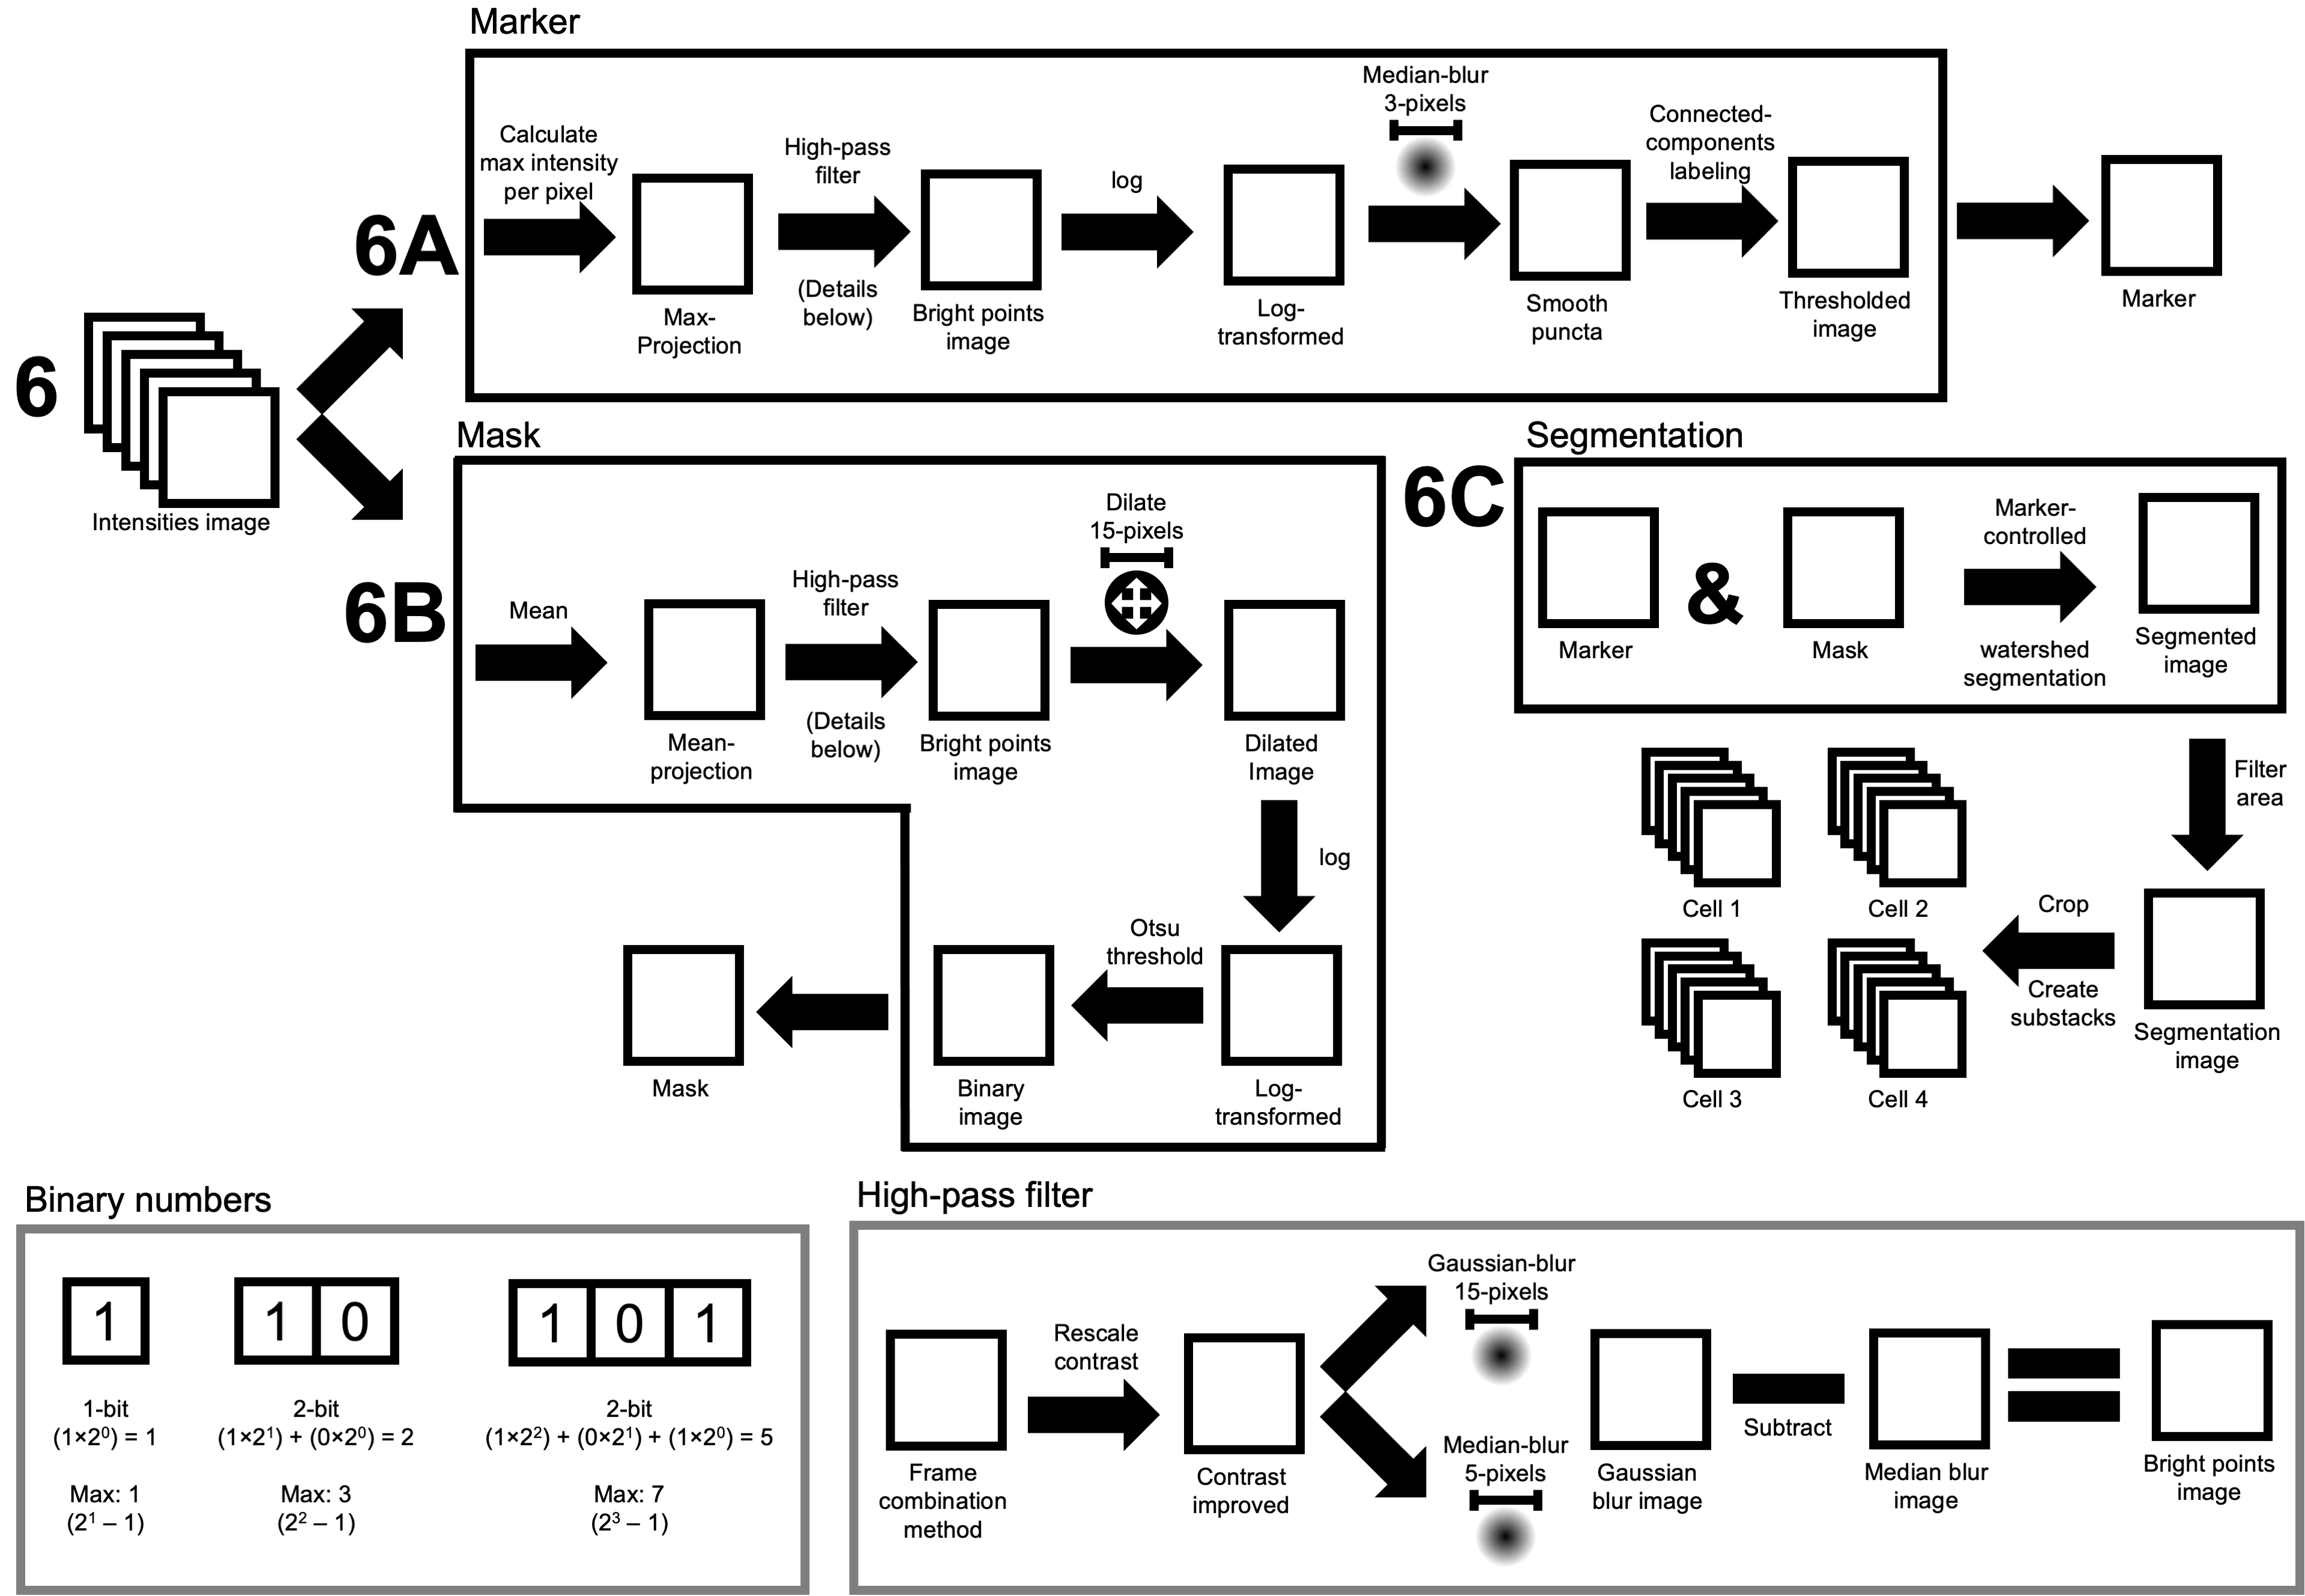
\includegraphics[height=\textwidth, width=\textheight, angle=-90, keepaspectratio]{methods/fig3.png}}}
\captionsetup{parbox=none}
\captionof{figure}[Cell segmentation is performed for calculating biological replicates and speeding-up the pipeline]{\textbf{Cell segmentation is performed for calculating biological replicates and speeding-up the pipeline.} For the segmentation method that I used, I needed to create two images, termed the marker and the mask. The marker indicates where a cell is while the mask indicates the boundary edges.
\\
\\
(6A) The marker is calculated by identifying the brightest regions in the cell. Then, the contrast is improved.
\\
\\
(6) The contrast adjustment rescales the images depending on the TIFF bit depth. This schematic shows how binary numbers (0 or 1) are converted to decimal (1 to 10).
\\
\\
(6B) The mask I used was determined by first averaging all the intensities per pixel. The resulting image, called the mean projection, has its contrast adjusted. The images are split again, one for calculating the Gaussian and another for calculating the median blur. The purpose of this is to calculate the edges. Gaussian blurs blow up images, whereas median blurs keep the structure, that is, they are edge preserving. The Gaussian is subtracted from the median. The resulting image is then log transformed to even out the cell illumination. Lastly, this image is converted into a binary using Otsu thresholding. (6C) For segmentation, I used an algorithm called marker-controlled watershed segmentation. This is a derivation of the watershed segmentation. Watershed segmentation identifies dips in intensities (i.e., local minima, valleys) to identify boundaries/edges. The marker-controlled watershed uses this, but it also uses the bright intensities (i.e., local maxima, hills) to identify how many regions (cells) there are inside the image. The resulting image is the segmentation image. The large original image is then cropped into smaller images using the segmentation image. These smaller images are of individual cells.}
\label{m:3}
\end{centering}

\subsection{TrackMate detects and tracks puncta}
\subsectionmark{TrackMate}
I tracked the puncta with TrackMate \autocite{Tinevez_2017}, an ImageJ plugin. The first step TrackMate takes is identifying all the puncta in a frame. This is called spot detection. To detect spots, it first fits a 2D Gaussian curve to the entire frame, that is, it applies a Gaussian blur to smooth the image because the next step uses changes (derivatives) in intensity, which are sensitive to noise (Fig.~\ref{m:4}.7A).
\begin{equation*}
f(x,y) =\text{exp}(-x^2 - y^2)
\end{equation*}
The change in intensity is calculated from one pixel to the next. This is known as the derivative (from calculus). \begin{equation*}\frac{dx}{dt} = \frac{int - int_0}{t - t_0} = \dot{int}\end{equation*} After, it calculates the change of the change, that is, the second derivative using a Laplace operator. \begin{equation*}\Delta f = \nabla^2 f = \nabla \cdot \nabla f\end{equation*} The Laplace operator is an algorithm for identifying edges (Fig.~\ref{m:4}.7A). The result is inverted and the local maxima (brightest pixels in a region) is used to mark the centroid of the puncta and then dilates it to fit a circle of a given pixel size, which for this pipeline is 5-pixels in diameter. This entire method is called Laplacian of Gausian (LoG) filter (Fig.~\ref{m:4}.7A). TrackMate then generates a table of puncta (called spots by the software) with xyt (horizontal, vertical, time) coordinates.

To establish which puncta size, there are some important considerations. Merging channels (as shown in the tracking step) introduces a new problem: the channels could potentially be misaligned. Having explained that TrackMate is sensitive to distances, if the spot size parameter is set too tight, part of the puncta would potentially be excluded. For Results~\ref{chapter:p1}, I used 0.44 µm (3-pixel) for the puncta diameter. However, puncta are highly dynamic, exhibiting constant merging and splitting. For this and subsequent chapters, I defined the puncta diameter as 0.73 µm (5-pixels). This allows for more movement flexibility, but a compromise had to be made in that if two puncta are too close, one runs the risk of not being detected.

The next step is to calculate the cost, that is, look at the different frames to identify which puncta are the same. Cost is calculated using the xyt coordinates of each spot to measure the distance to the spots in the next frame (Fig.~\ref{m:4}.7B). One distance method used is Euclidean distance. \begin{equation*}d(x, y) = \sqrt{(x_{1} + x_{0})^2 + (y_{1} + y_{0})^2}\end{equation*} This is done for all puncta, though algorithms take shortcuts to calculate these distances more efficiently, for example, neighbor search. Additionally, criteria are applied, including the intensities.

The closest puncta between frames would be considered to be the same puncta, and the process to identify this is called the linkage. The set of puncta in different frames but considered to be the same are called a track (Fig.~\ref{m:4}.7B). The algorithm that I used from TrackMate is called the simple linear assignment problem (LAP) (Fig.~\ref{m:4}.7B). An assignment problem is a combination optimization method that finds the best set of puncta that are similar. TrackMate uses additional criteria to find puncta. The first is filtering out spots in different frames that are too far apart. This is called the linking max distance. TrackMate also allows spots to be missing in some frames. This accommodates phenomena like fluorophore blinking. The number of frames that can be skipped is called the gap-closing max frame gap. The maximum linking distance between gaps is called the gap-closing max distance. After running the different algorithms, TrackMate is told to save the files. It uses the extended module (XML) file format (Fig.~\ref{m:4}.7C).


\begin{centering}
\bigfig{\centering{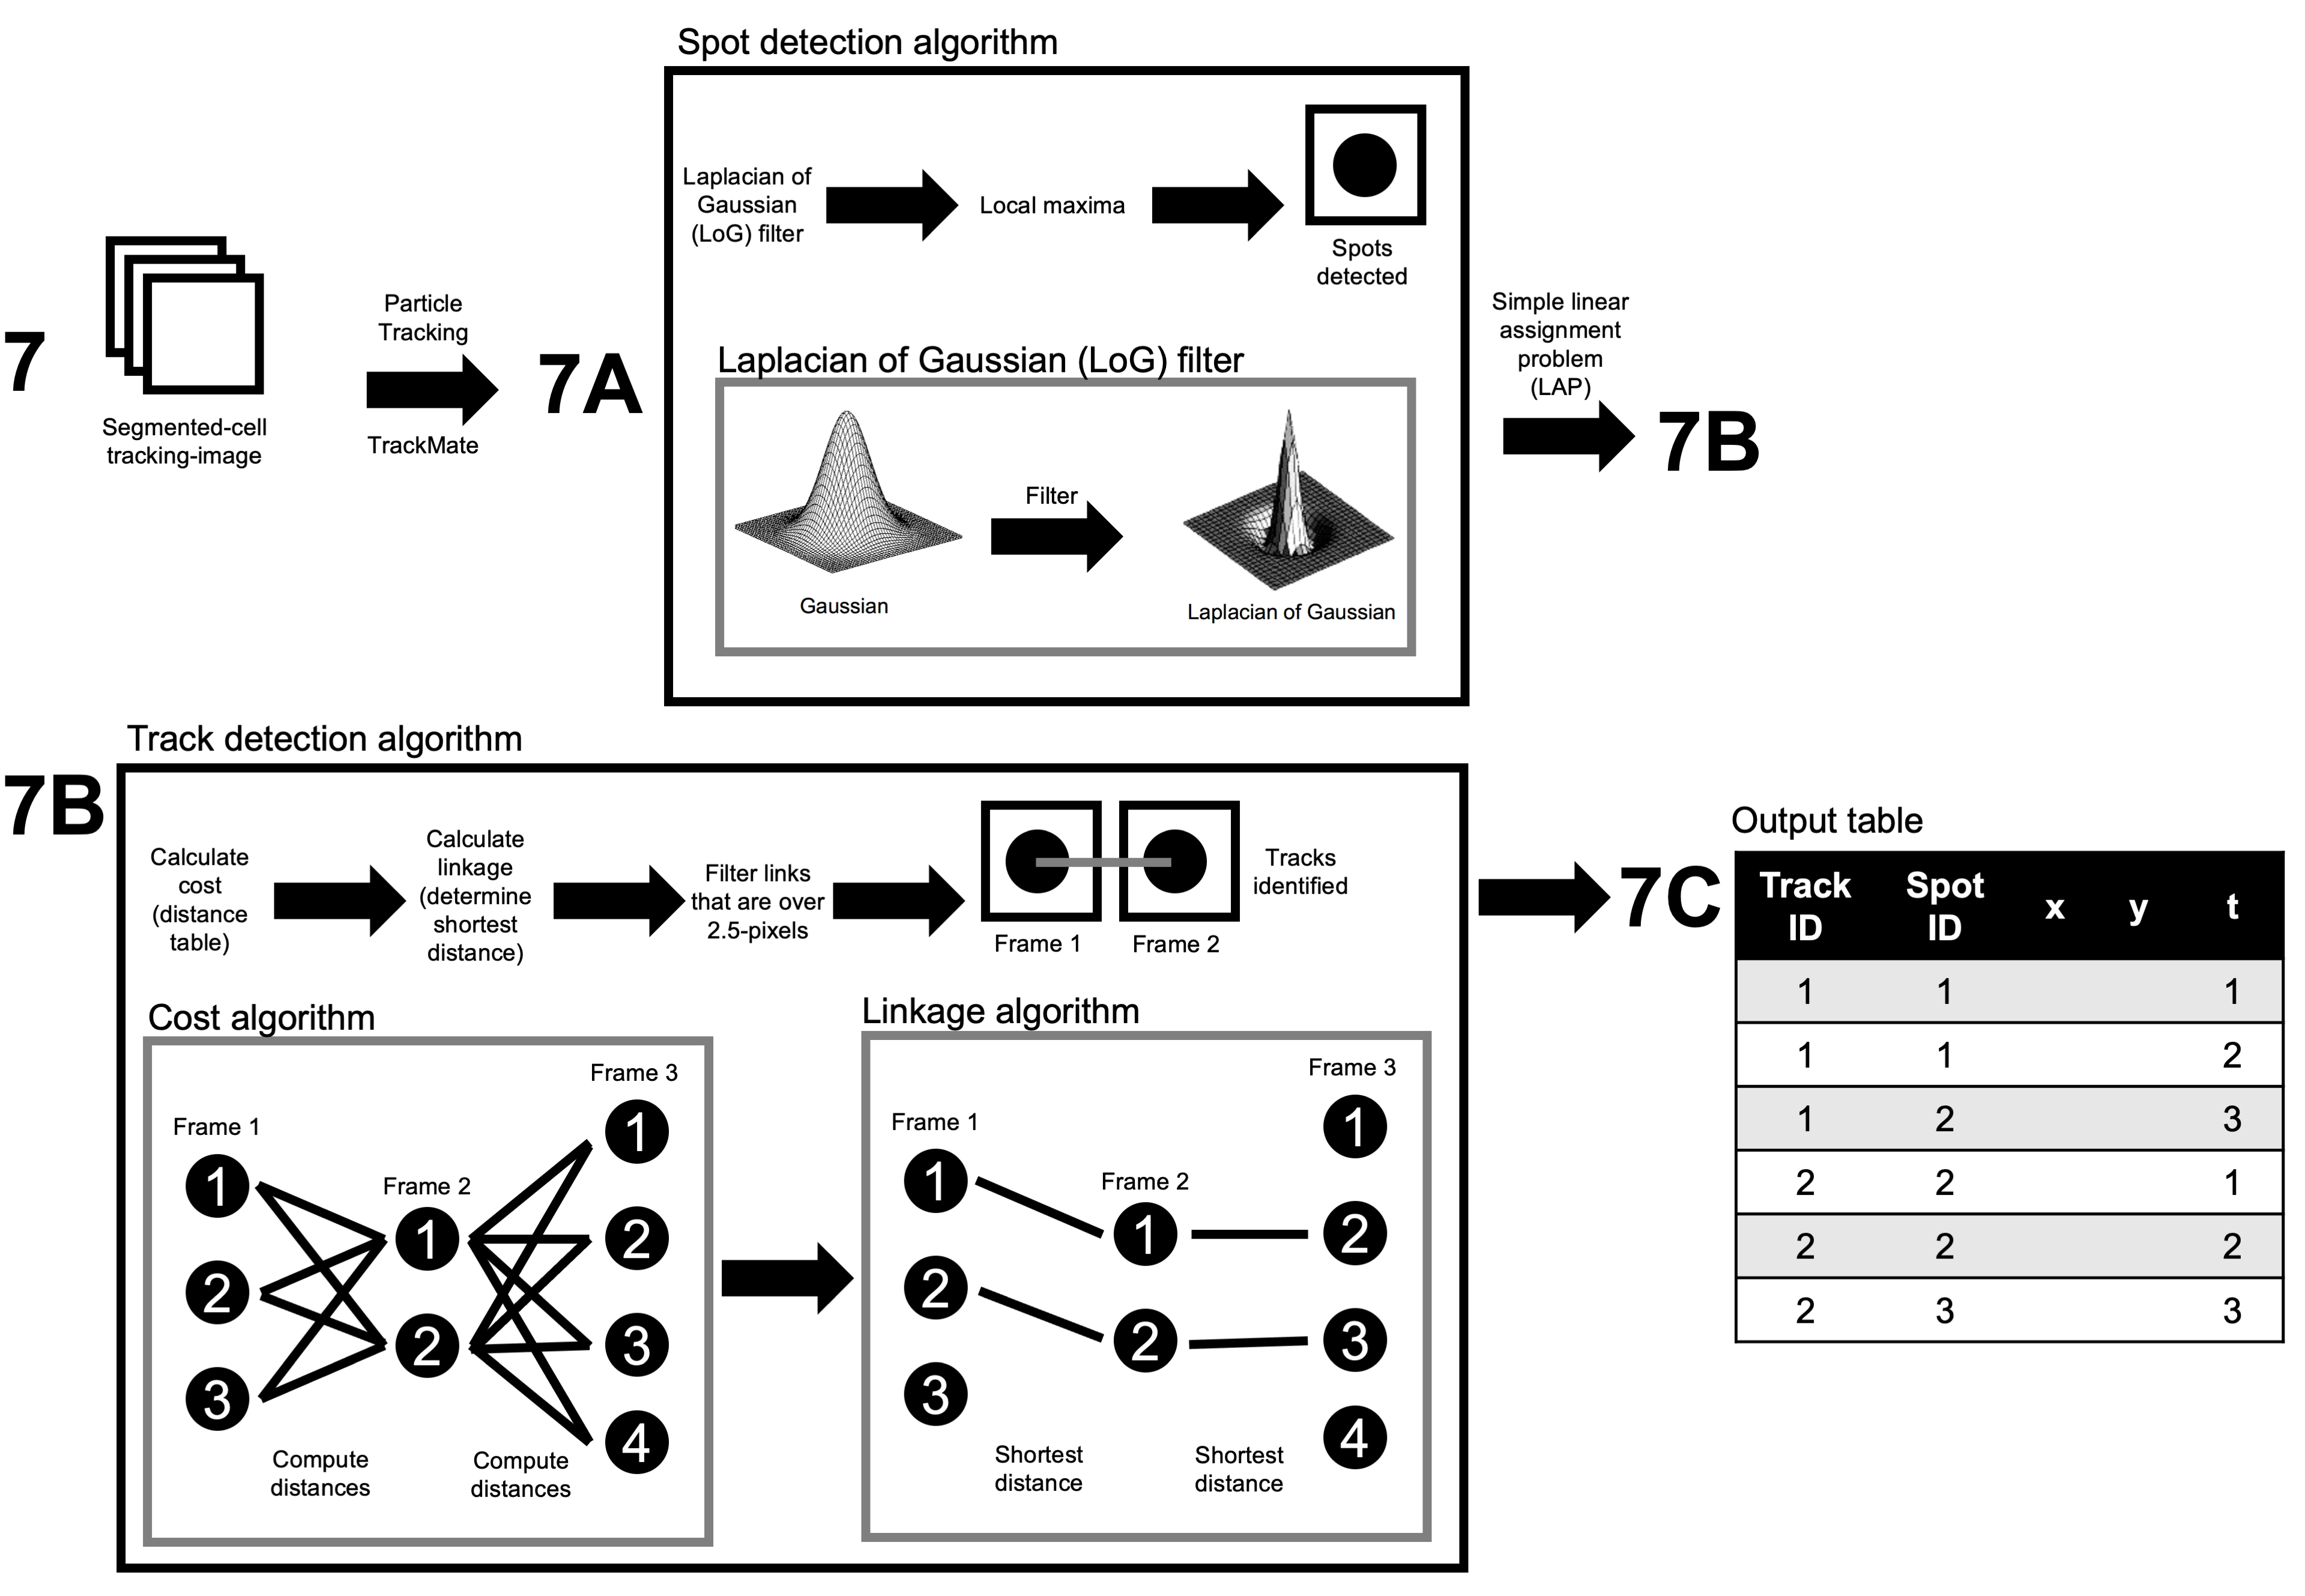
\includegraphics[height=\textwidth, width=\textheight, angle=-90, keepaspectratio]{methods/fig4.png}}}
\captionsetup{parbox=none}
\captionof{figure}[Puncta were identified using TrackMate]{\textbf{Puncta were identified using TrackMate} I used TrackMate to detect puncta and its movements.
\\
\\
(7) The segmented images containing individual cells were fed into the TrackMate plugin of ImageJ.
\\
\\
(7A) The first algorithm TrackMate uses is for detecting puncta. TrackMate calls these spots. It uses a Laplacian of Gaussian filter. This fits a Gaussian (normal) curve and then calculates the edge using a Laplace operator (a differential equation as in Calculus). Lastly, it identifies the local maxima and puts a circle with a defined diameter, 5-pixels in the case of my pipeline. A large table of spots is generated. However, this does not tell us the puncta dynamics, that is, how the puncta grows and shrinks, when it appears and disappears. For this, I need to link puncta in a process TrackMate calls track detection.
\\
\\
(7B) Puncta split and merge, and while there are available TrackMate methods that account for this, this makes the data analysis exponentially more challenging to work around with. It is for simplicity's sake that I used the aptly called simple linear assignment problem (LAP) method for the track detection method. The first step in identifying tracks is to calculate what is called the cost. The cost is the distance between puncta from one frame to the next. For example, in frame 1, I have puncta 1. I calculate its distance to all the puncta in the next frame (Frame 2), that is, puncta 1 and puncta 2 of frame 2. This is done iteratively for all puncta. There are shortcuts algorithms use for calculating cost efficiently. More on this at \autocite{Tinevez_2017}. Using the cost table, the algorithm then calculates the link. That is, it tries to identify the shortest distance. TrackMate allows the user to set a maximum link distance which goes by the same name. Lastly, this is all tabulated and identifies tracks.
\\
\\
(7C) The output information is saved in an XML file which I later extract its data to convert it into a table.}
\label{m:4}
\end{centering}

\subsection{Intensities are measured from the intensity image using TrackMate coordinates}
\subsectionmark{Intensity measured}
Now that the puncta have been tracked in the tracking image, the next step is extracting the fluorescent intensities for the puncta in the different intensity reference images. This is done using R. It is worth mentioning that tracking was done in an image that combines all channels. With this step, channel-specific information is gathered.

The output TrackMate provides is an XML file. I need to convert the XML puncta information into a table, so that it can be easily manipulated in R. TrackMate saves the puncta and track information separately. I extracted the puncta information and paired it with the track information using the puncta (spot) identifiers.

TrackMate allows skipping frames. To fill in the void, I approximated the location of the missing puncta using Euclidean distance. \begin{equation*}d(x, y) = \frac{\sqrt{(x_{1} + x_{0})^2 + (y_{1} + y_{0})^2}}{n_\text{gap size}}\end{equation*}

With all xyt coordinates available, I extracted the intensities from the intensities reference image. I converted the TIFF image into a matrix. Then, I crop out a square around the puncta (including the puncta). TrackMate used the LoG algorithm to calculate with sub-pixel accuracy the centroid of the puncta. This means I cannot take the centroid of the matrix, draw a circle around it, and sum it. This would offer pixel-level accuracy.

To calculate with sub-pixel accuracy the intensities of the images, I took a different approach. The aforementioned cropped matrix was blown-up, so that I can later use integers to filter-out pixels. I scaled-up (expanded) the image square matrix eleven times ($k = 11 \times$). I chose this factor because this estimation method is 0.387\% similar to a matrix of $k = 51 \times$. I also tried the faster $k = 5 \times$, and it is off by 0.571\% (versus $k = 51 \times$). While it may seem insignificant, error propagates. $k = 11\times$ diminishes the error by 51\%.

Puncta are circular. To segment puncta, I had to generate a circular mask (binary outline, like explained in the segmentation step). I used the equation of a circle \begin{equation*}\sqrt{x^2 + y^2} = r\end{equation*} and adapted it so that I can make a matrix of pixels with a circle inside a square. \begin{equation*}[x - x_0]^2 + [y - y_0]^2 \le r^2\end{equation*} This is done because the puncta right now is in a square matrix (generated earlier). However, this equation does not account for the expansion. Therefore, I added a constant $k$ to dilate (blow-up) the circle matrix by a factor of $11\times$ ($k$), so that it has the same dimensions as the blown-up image matrix.

$\begin{aligned}
\relax[x - (r \cdot k)]^2 + [y - (r \cdot k)]^2 &\le (r \cdot k)^2\\
[x - (5\text{ px} \times 11)]^2 + [y - (5\text{ px} \times 11)]^2 &\le (5\text{ px} \times 11)^2 \\
\sqrt{[x - 55\text{ px}]^2 + [y - 55\text{ px}]^2} &\le 55\text{ px}
\end{aligned}$
The resulting matrix was converted into binary:
\begin{equation*}
\text{mask}(x,y) =
\left\{\begin{array}{lr}
0, & \text{if }d(x,y)\le (r\cdot k)\\
1, & \text{if }d(x,y) > (r\cdot k)
\end{array}\right.
\end{equation*}
where $d(x,y)$ is the pixel in question.

This binary matrix mask is multiplied by the image. The output is a segmented punctum. Multiplying times zero makes the image black and multiplying times one means the input image intensity is kept. This allows me to sum the intensities of the segmented punctum. I then recorded this numerical output as the puncta intensity for a specific channel.

Previously, I had saved the metadata and extracted meaningful information out of it (e.g., TIRF angle, date, proteins in each channel). Now, I combine the metadata, the TrackMate information, and the intensities into a single table. A detailed table content is available in the Methods chapter. I saved this in a comma separated values (csv) table and compressed it using gzip. The intensities of the different channels are added to each spot row using a separate script.

\subsection{The signal is normalized using monomeric fluorophores to estimate puncta stoichiometries}
\subsectionmark{Signal normalization}
\label{subsection:normalization}
The pipeline is now able to self-calibrate (pairing monomeric fluorophore intensities with experimental images obtained in similar conditions) without user input. When we image cells at the microscope (experimental image), we also take images of monomeric fluorophores (calibration image) using the same parameters (angle, direction, laser power, exposure) as the cell imaging. This is done so that I can normalize (calibrate) the experimental images to a reference standard. These calibration images are processed the same way as the experimental images. Then, the pipeline identifies the median brightness of the fluorophore and uses this for normalization by division. The resulting quotient offers an approximation of the stoichiometry (assembly size, oligomer length) in a diffraction-limited puncta which enables us to compare it to other methods (e.g., solved crystal structures).

To automatically determine which calibration image to use, the pipeline uses the metadata of the calibration and experimental images. It pairs the channel name of the calibration and experimental images. For each experimental image, it identifies the best calibration image using the following hierarchy (priority):
\begin{enumerate}
\item Power,
\item Exposure,
\item Angle (in radians),
\item Direction, and
\item Date.
\end{enumerate}
For each step, it calculates the absolute difference between the images metadata, and selects the nearest value before proceeding to the next element in the hierarchy. After it finds the nearest value, it normalizes the intensity. \begin{equation*}int_{\text{normalized}} = \frac{int_{\text{punctum}}}{int_{\text{monmeric fluorophore}}}\end{equation*}
Where $int$ is intensity.
\subsection{The ligand density is binned so that experimental replicates can be compared}
\subsectionmark{Ligand density}
Protein dynamics are affected by the amount of ligand available in the supported lipid bilayer. Too much ligand, and the assembly process cannot be seen because it happens too fast. This needs to be accounted for when comparing experimental replicates. For each experiment, I estimate the amount of ligand in the supported lipid bilayer. This is done by labeling the ligand with a fluorescent organic dye. Then, I count the number of molecules detected in the field of view and divide it by the area of the image. This is the ligand density. Then, I count the number of puncta seen in the first frames using TrackMate. Because these molecules are freely diffusing, they travel fast. This means motion blur is an issue (motion blur discussed above). The organic dye tolerates photons well. Therefore, I use the lowest exposure possible and the highest laser power that will not burn the camera. For a 16-bit camera, this limit should be be 49,151 a.u. (75\% of the max brightness).
\begin{equation*}
\begin{aligned}
\text{max brightness} &= 0.75 \times (2^\text{bit-depth} - 1)\text{ a.u.} \\
& = 0.75 \times(2^{16}-1)\text{ a.u.} \\
& = 0.75 \times (65,535\text{ a.u.}) \\
& = 49,151\text{ a.u.}
\end{aligned}
\end{equation*}

Sometimes, the field of view is dense and individual molecules cannot be counted. To address this issue, we dilute the ratio of labeled to unlabeled protein. Another approach is to capture images continuously to photobleach the molecules. Then, I fit a regression line and use the equation parameters to estimate how many molecules were present at the very beginning. 

From my observations, I have seen that the amount of ligand causes exponential shifts in the protein dynamics. To make this nonlinear system linear, a transformation is in order. Because the data is exponential, a log-transformation will make the ligand density linear. I used $\\log_{\sqrt{10}}(\text{ligand density})$. However, the ligand density must be binned in log-scale.
\begin{equation*}
\begin{aligned}
\text{ligand density}_\text{category} &\approx \log_{\sqrt{10}}(\text{ligand density})\\
&\approx \frac{2 \cdot \log(\text{ligand density})}{\log(10)}
\end{aligned}
\end{equation*}

\subsection{The data gets tabulated and saved}
\subsectionmark{Saving the data}
Users have expressed interest in filtering puncta that have other puncta nearby to account for splitting and merging. To add this functionality, the pipeline calculates the distance to the nearest spot, and the number of spots within a distance ($d_\text{search}$) using the nearest neighbor search algorithm. The distance threshold ($d_\text{search}$) is calculated using using the equation:
\begin{equation*}
d_\text{search} = 6\cdot d_\text{puncta}
\end{equation*}

After completing all this, the output is saved in a compressed csv file. CSV files are read row-wise. This means that a lot of unnecessary variables are sometimes read. While I saved different tables with different variables (see Methods~\ref{section:output_tables}), the issue remains. One approach would be to save the table in a format that reads column-wise. One such format is parquet. The installation can be tedious, which is why I did not opt for it (up to this step).


\begin{centering}
\centering{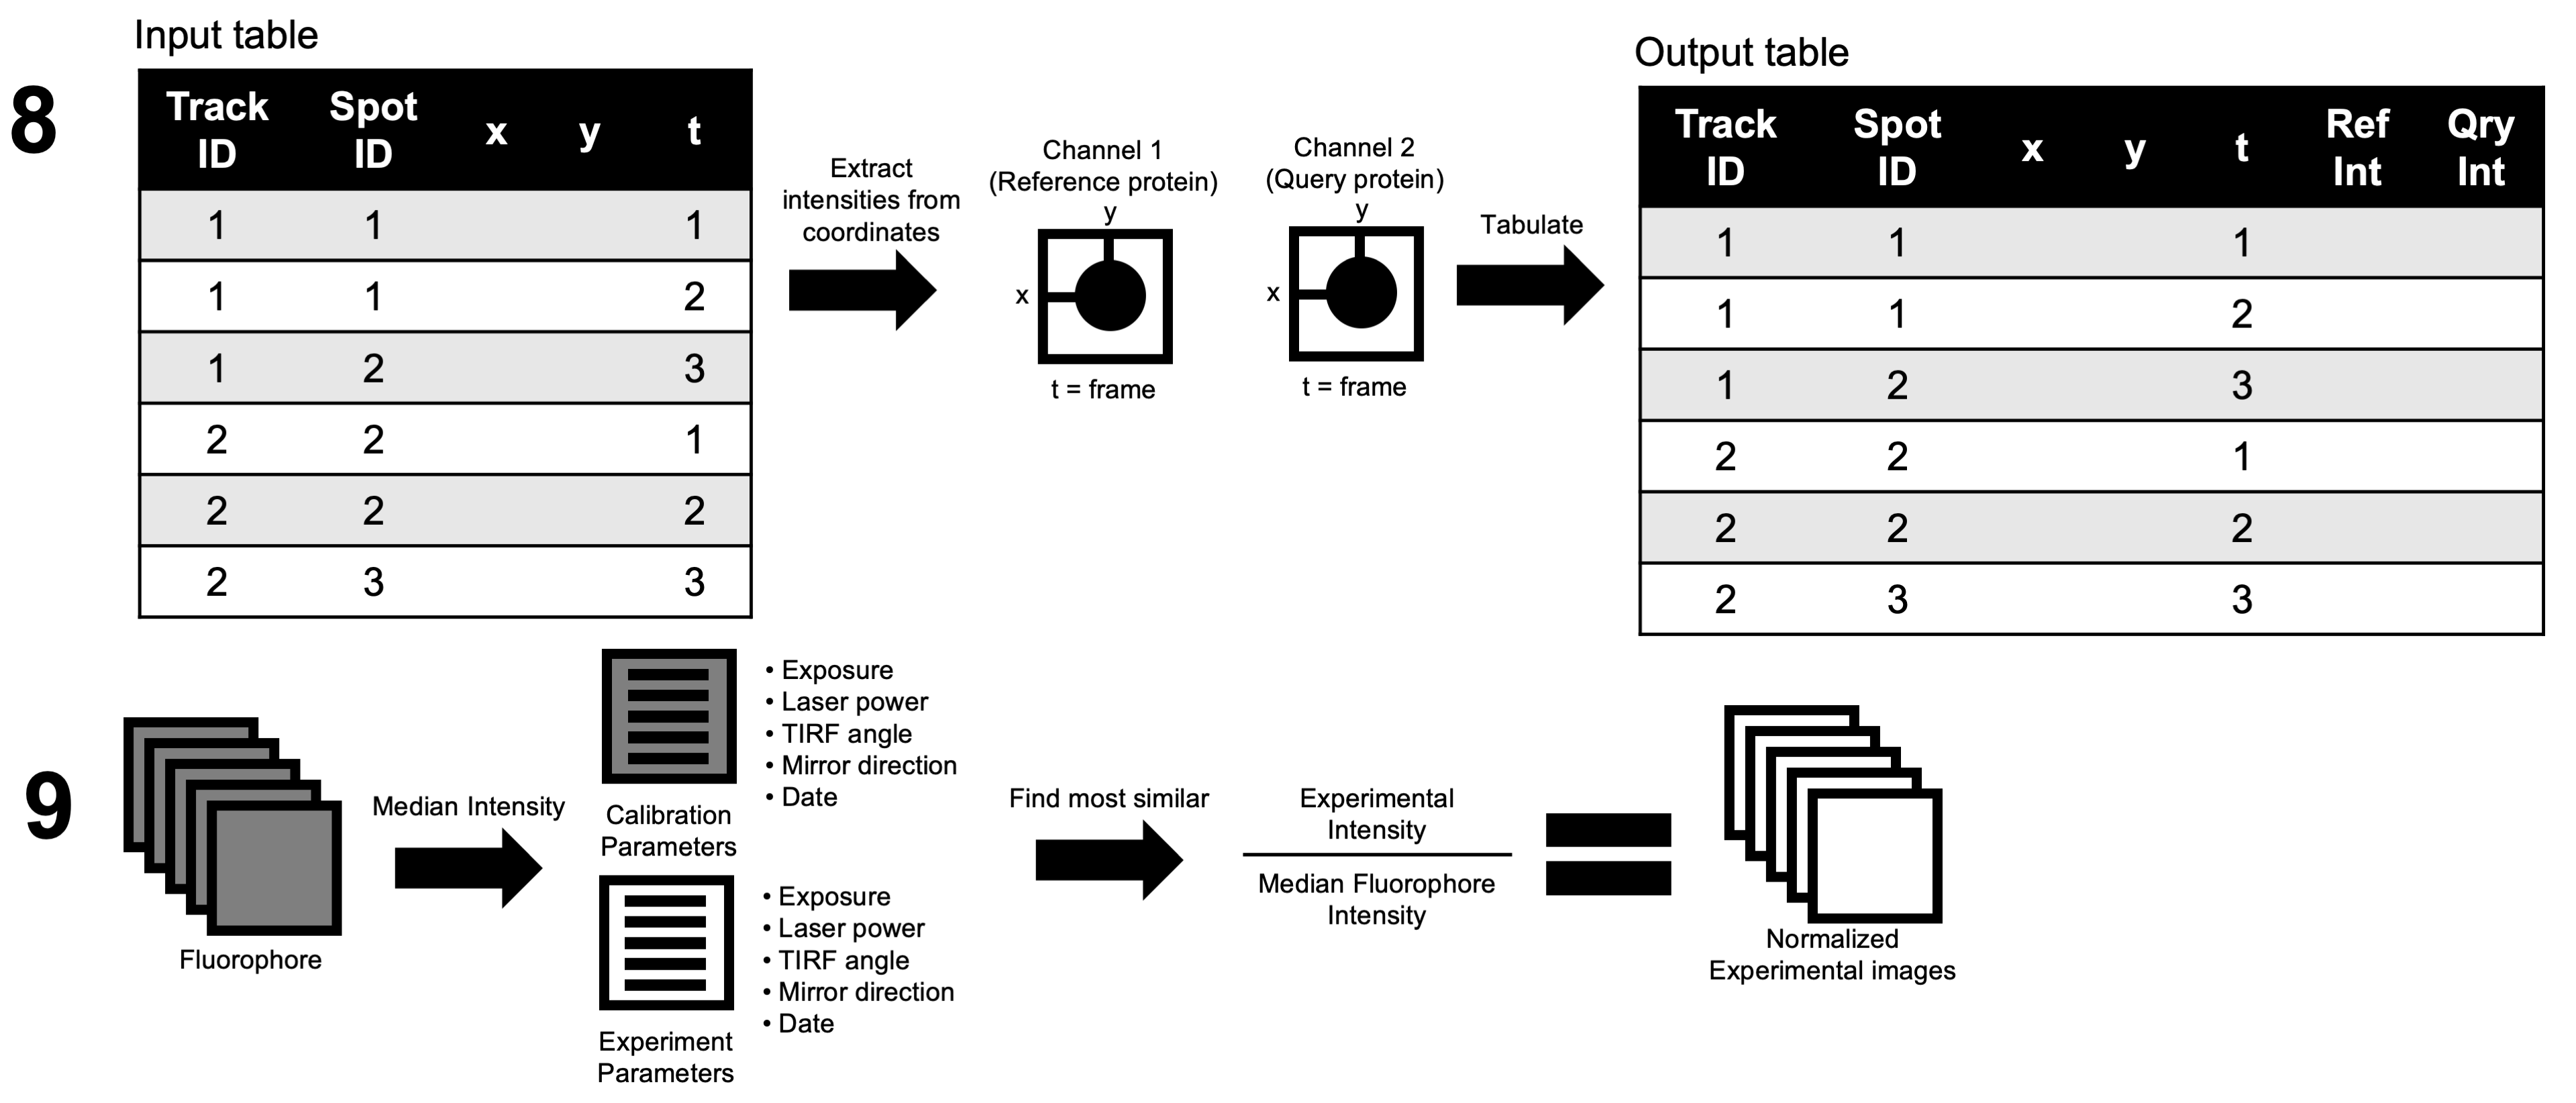
\includegraphics[height=\textwidth, width=\textheight, angle=-90, keepaspectratio]{methods/fig5.png}}
\captionsetup{parbox=none}
\captionof{figure}[Intensities are extracted from TrackMate coordinates, normalized using the calibration monomeric fluorophores, and saved into a table]{\textbf{Intensities are extracted from TrackMate coordinates, normalized using the calibration monomeric fluorophores, and saved into a table}
\\
\\
(8) TrackMate generated a list of xyt coordinates. To obtain the punctum intensity, I segmented circles out of the different channel images, and used the sum of the pixel intensities per channel as the punctum intensity.
\\
\\
(9) Intensities are in arbitrary units. To be able to compare replicates, as well as the stoichiometry of images against that of solved crystal structures, I normalized the signal to the intensity of monomeric fluorophores. The resulting normalized intensity roughly correlates with the actual stoichiometry of puncta.}
\label{m:5}
\end{centering}

While the scripts compress images, the files can be large. A script is provided to compress everything. This also speeds up the data transfer as too many files slows transfer due to overhead processes.

\subsection{Complex systems can be studied using dimensionality reduction}
\subsectionmark{Complex systems}
\label{section:complex}
Complex systems are intrinsically difficult to understand and model because they can be non-linear, that is, the input-output relationship is not proportional (linear). Instead, it can appear random and unpredictable. Complex systems typically involve multiple components which interact with each other. The protein dynamics I observed can be described as a complex system. In this system, these components are proteins. Complex systems can exhibit feedback, and spontaneous order.

To capture trends, data needs to be summarized while keeping heterogeneity. Two methods through which complex systems can be untangled involve phase portraits and dimensionality reduction.

Dimensionality reduction is the transformation through which high-dimensional space is converted into a low-dimensional space while still retaining the properties of the high-dimensional data. Dimensionality reduction summarizes information by identifying the most important features, and analyzing them. One of the best known dimensionality reduction tools used in biology is principal component analysis (PCA). Dimensionality reduction is particularly useful for complex systems for drawing conclusions when multiple variables influence each other.

Phase portraits are plots of the trajectories of dynamical systems (see Intro~\ref{section:pp}. With the phase portrait, I can identify thresholds, equilibrium points, and regulatory mechanisms.

\subsection{Puncta colocalization can be studied using phase portrait analysis}
\subsectionmark{Phase portrait analysis}
\label{section:pp_method}
The puncta have been measured, but this is only part of the story. To understand how proteins interact with each other within the diffraction-limited puncta, the data needs to be analyzed. I was interested in the dynamics of protein colocalization. Classical protein colocalization microscopy has used correlations between protein intensities per pixel (pixel-matching). The issue here is that dynamics are lost. It is also highly susceptible to noise. Sometimes, a filter is applied so that only the bright pixels of the image are used. Classic colocalization has also used object masking (binary images) to then determine the Manders’ split coefficients. It then calculates the percent overlap from the perspective of each channel. Here, the issue is that the image needs to be thresholded. A decision needs to be made whether it counts or not. Therefore, it has high potential for user bias.

The previous pipeline paired puncta using coordinates, and then looked at their intensities. I made comparisons using the lifetime of the reference protein (MyD88) and the percent colocalization. I also asked how bright the reference protein needs to be to recruit a downstream protein. I calculated the delay between one puncta appearing and the next. However, this approach makes generalizations about the puncta.

I looked at over nine IL-1 pathway proteins. This means my system has nine dimensions. The dynamics are heterogeneous, and not linear, which means the pathway is a complex system. To better understand how individual protein puncta make decisions, I took a soft matter physics approach.

For my phase portraits, I plotted the proteins in phase space, that is, I used the oligomer length of a reference protein (MyD88) and compared it against a query (downstream) protein. I binned the x and y axis using a step size of every 3\times oligomer length. I chose this step size because the trajectories are clear with minimal noise. If there were less than 125 puncta meeting this criteria, then the data was filtered out. This removes noisy data which is not representative of the protein dynamics. The noise can potentially be a random flux which is a type I error (false positive) as a result of poor precision in measurements, and not a true measurement. This filter also focuses the attention of the user into the most frequent events.

Interested in protein assembly, I calculated how each protein grows. The next step involved calculating the change in intensity, that is, the derivative of puncta (Fig.~\ref{m:6}). I used a window of $\pm5$ frames, meaning I took a puncta and asked, what was the intensity at five timepoints before and after. I took the difference between these two intensities and the result is the change in intensity (Fig.~\ref{m:6}).
\begin{equation*}
\Delta int = (\Delta {int}_{t =t_0+t_5}) - ({int}_{t =t_0-t_5})
\end{equation*}
To add this to the phase portrait, I looked at all the puncta that met the criteria of a bin, and asked, what is the median intensity change for each protein. The magnitude of growth was indicated using color in the arrows.
\begin{equation*}
\text{magnitude} = |\Delta_\text{reference protein}| + |\Delta_\text{query protein}|
\end{equation*}
Magnitudes are absolute values. That means it does not differentiate between growth and shrinkage. To account for this, I used the arrow angle to indicate which protein is growing or shrinking. The angle was calculated using the two argument tangent of the change in intensity.
\begin{equation*}
\begin{aligned}
\theta &= \text{atan2}(\Delta_\text{query protein}, \Delta_\text{reference protein})\\&=
\left\{\begin{array}{ll}

\text{arctan}(\frac{\Delta_\text{query protein}}{\Delta_\text{reference protein}}), & \text{if }\Delta_\text{reference protein} > 0\\

\text{arctan}(\frac{\Delta_\text{query protein}}{\Delta_\text{reference protein}})+\pi, & \text{if }\Delta_\text{reference protein} < 0 \text{ and }\Delta_\text{query protein} \ge 0\\

\text{arctan}(\frac{\Delta_\text{query protein}}{\Delta_\text{reference protein}})-\pi, & \text{if }\Delta_\text{reference protein} < 0 \text{ and }\Delta_\text{query protein} < 0\\

+\frac{\pi}{2}, & \text{if }\Delta_\text{reference protein} =0 \text{ and }\Delta_\text{query protein}>0\\

-\frac{\pi}{2}, & \text{if }\Delta_\text{reference protein} =0 \text{ and }\Delta_\text{query protein}<0\\

\text{undefined}, & \text{if }\Delta_\text{reference protein} =0 \text{ and }\Delta_\text{query protein}=0

\end{array}\right.
\end{aligned}
\end{equation*}


\begin{centering}
\centering{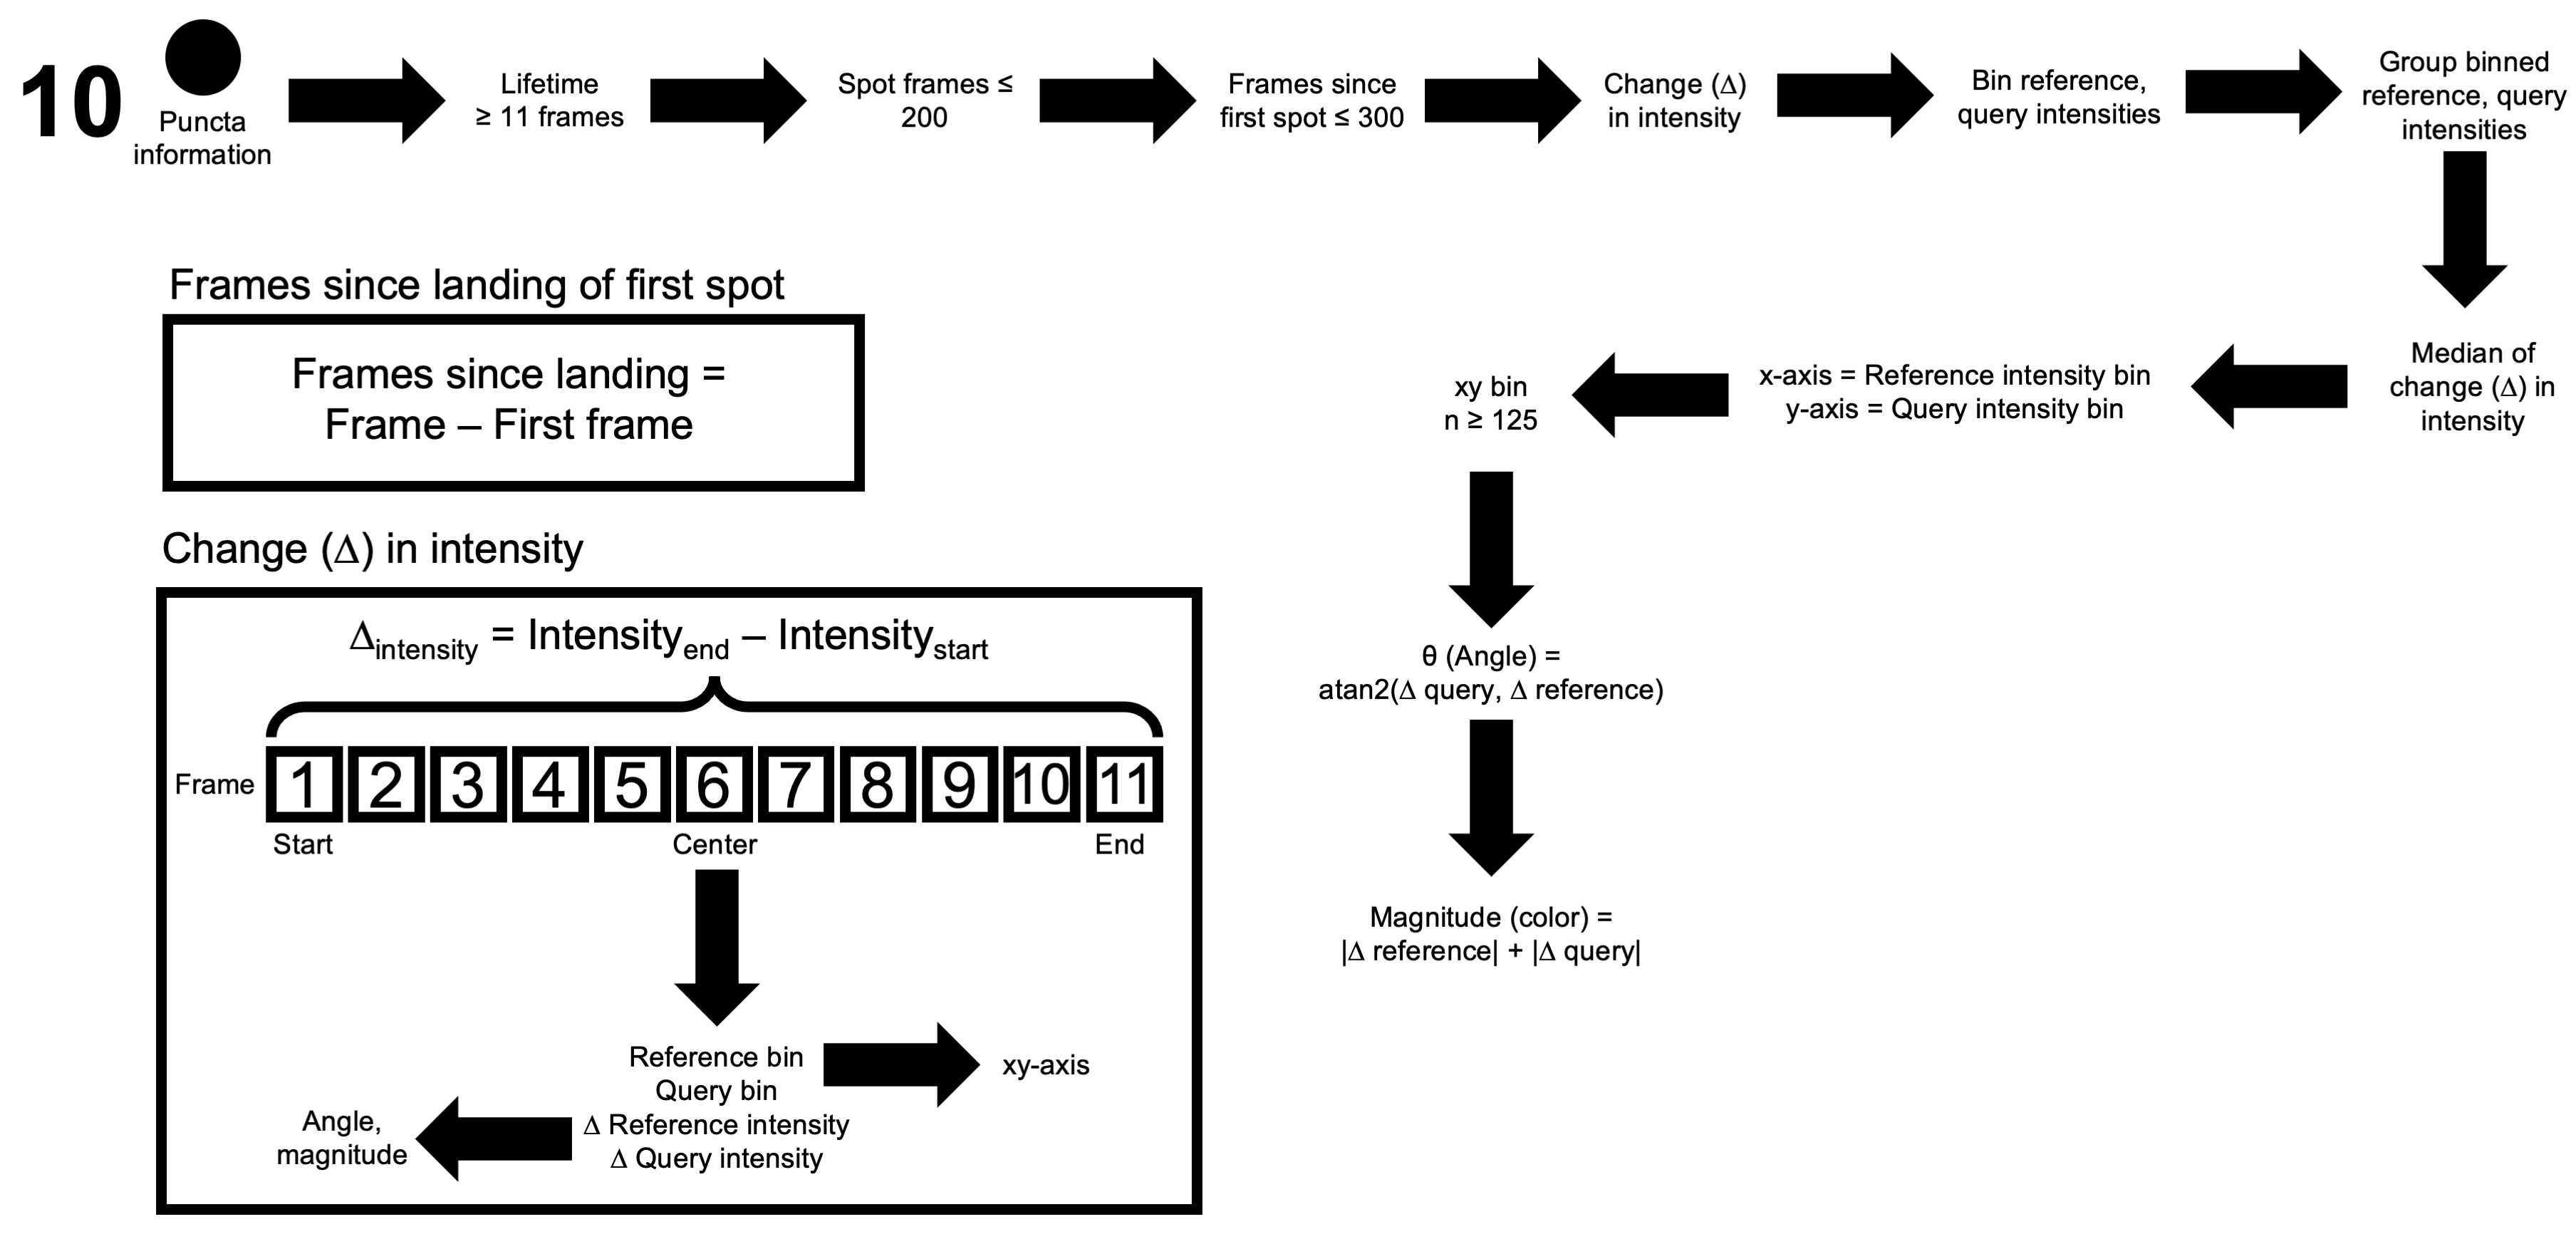
\includegraphics[height=\textwidth, width=\textheight, angle=-90, keepaspectratio]{methods/fig6.png}}
\captionsetup{parbox=none}
\captionof{figure}[Colocalization using phase portrait analysis can reveal protein dynamics]{\textbf{Colocalization using phase portrait analysis can reveal protein dynamics.} I used phase portrait analysis to analyze the dynamics of protein colocalization. I filtered data so that only puncta with lifetimes over 11 frames (44 s) are included. Then, only the first 200 frames of each puncta were included in the analysis. Another filter limited puncta, so that only those within the first 300 frames since the first spot appeared (frames since landing, see insert) are included. After, I calculated the change in intensity, looking five frames back (lag) and five frames forward (lead) (see insert). The difference in intensities is then recorded per punctum, along with the normalized intensities of the reference and query proteins at the center value. For each binned (every 3\times normalized proteins, per channel) intensity pair (reference, query), I calculated the average (median) change in intensity. Only bins with more than 125 puncta were included. I used the two-argument tangent to calculate the angle of the phase portrait arrow, and the sum of the absolute change in intensities as the arrow magnitude which is indicated in the phase portrait color. The final output is a phase portrait.}
\label{m:6}
\end{centering}

To increase the number of observations, I combined images with similar dynamics. I separated the proteins based on the ligand density (as explained before) because this simple binning method showed similar protein dynamics. To confirm this, I drew the average protein size over time (time traces), color coding the image replicates. After visually confirming that the images show similar dynamics, I rescaled the data using min-max normalization:
\begin{equation*}
int_\text{scaled} = \frac{int - int_{1^{st}\,\%}}{int_{99^{th}\,\%} - int_{1^{st}\,\%}}
\end{equation*}
and then identified the median min-max values. I used the image whose min-max values were the closest to the median to give normalized values.
\begin{equation*}
int_\text{final} = int_\text{scaled} \times int_{99^{th} \%_\text{median}}+int_{1^{st} \%_\text{median}}
\left\{\begin{array}{lr}
0, & \text{if }int_\text{final} < 0\\
int_\text{final}, & \text{if }int_\text{final} \geq 0
\end{array}\right.
\end{equation*}
That is, the median calibration values were used to normalize intensities to stoichiometric estimates.

\subsection{The pipeline is parallelized to speed up the analysis}
\subsectionmark{Parallelization}
The previous pipeline used ImageJ for image processing. One drawback of ImageJ is that few of the processes I used are parallelized, TrackMate being the exception. For this reason, I had to translate the ImageJ functions (for example, file format conversion, median blur) into Python. I used Ray to parallelize my Python scripts, and parallel to parallelize my R scripts. I wrote the scripts so that they can run on Mac, Linux and Windows operating systems (OS). This means the scripts can now run on UNIX-based (OS) high-performance computers (“super-computers”).

I used single nodes from the Raven high-performance computer (HPC) of the Max Planck Computing and Data Facility (MPCDF), Garching, Germany (CPU: 72 cores @ 2.4 GHz, Intel Xeon IceLake Platinum 8360Y; RAM: 256 GB). I also successfully tested it with Cobra of the MPCDF, Garching, Germany (CPU: 40 cores \@ 2.4 GHz, Intel Xeon Gold 6148 Skylake; RAM: 96 GB).

\subsection{Additional improvements to the image analysis pipeline}
\subsectionmark{Additional improvements}
The previous pipeline had over eight scripts that ran independently. It has all been consolidated into one master script that combines Python, ImageJ and R. The image preprocessing (file type conversion, background subtraction) is done in Python using OpenCV, and parallelized with Ray. Puncta are tracked in ImageJ using TrackMate \autocite{Tinevez_2017}. Lastly, the signal normalization, data consolidation (into one table), and plotting is done in R.

\section{Executing PIRATES: Pipeline for Image analysis with Reference images, Automated Tracking, Extraction of intensities, and Segmentation}
\label{section:PIRATES}
\sectionmark{PIRATES}
I developed a second improved image analysis pipeline for quantifying microscopy images. The second pipeline makes extensive use of parallel processing. It was written in Python 3.8.5, FIJI/ImageJ2 v2 \autocite{Schindelin_2012}\autocite{Rueden_2017} and R 4.0.2 \autocite{RCoreTeam_2020}, and runs on puncta computers.

More details on the pipeline rationale is available in Methods~\ref{chapter:PIRATES_PARLEYS}. Here, I share which scripts are needed and how to enter (input) the parameters into the pipeline.

The pipeline scripts are deposited on GitHub (\url{https://github.com/rhdeliz/puncta-dynamics}). 

\subsubsection*{Input}
The input data goes into ~/new\_pipeline/pending\_processing/batch\_date/Input/

\begin{table}[htb]
  \centering
  \caption{Numbers which are constant throughout the analysis}
  \label{tab:constants}
  \begin{tabular}{ | l | c | p{5cm} | }
    \hline
    \textbf{Parameter} & \textbf{Value} & \textbf{Comments} \\ \hline
    \texttt{tiff\_compression\_level} & 5 & out of 10 \\ \hline
    \texttt{cell\_diameter} & 25 & px, odd number \\ \hline
    \texttt{puncta\_diameter} & 5 & px, odd number \\ \hline
  \end{tabular}
\end{table}

\begin{table}[htb]
  \centering
  \caption{The dark frame is the camera noise. This typically is 1000 frames averaged, though 50 frames could do, so long as the standard deviation does not change with more images added. It should be at the same exposure as the images using the same camera as the microscopy images. Thus, one image could be used for multiple channels.}
  \label{tab:dark\_frames}
  \begin{tabular}{ | l | c | }
    \hline
    \textbf{Image} & \textbf{Exposure} \\ \hline
    \texttt{20201026 Darkfield 200ms binned.tif} & 200 ms \\ \hline
    \texttt{20201026 Darkfield 50ms binned.tif} & 50 ms \\ \hline
    \texttt{20201026 Darkfield 100ms binned.tif} & 100 ms \\ \hline
  \end{tabular}
\end{table}

\begin{table}[htb]
  \centering
  \caption{Directory paths}
  \label{tab:directories}
  \begin{tabular}{ | l | p{10cm} | }
    \hline
    \textbf{Contains} & \textbf{Path} \\ \hline
    \texttt{input} & \texttt{\textasciitilde/Input} \\ \hline
    \texttt{processing} & \texttt{\textasciitilde/Processing} \\ \hline
    \texttt{output} & \texttt{\textasciitilde/Output} \\ \hline
    \texttt{dark\_frames} & \texttt{\textasciitilde/dark\_frames} \\ \hline
    \texttt{flat\_fields} & \texttt{\textasciitilde/flat\_fields} \\ \hline
    \texttt{ImageJ} & \texttt{\textasciitilde/Fiji.app/ImageJ-linux64} \\ \hline
  \end{tabular}
\end{table}


\subsubsection*{exclusion\_channels.csv}
\begin{tabular}{|c|}
    \hline
    value \\
    \hline
    IL-1 \\
    Brightfield \\
    WideField \\
    \hline
\end{tabular}

\subsubsection*{images.csv}
See next page for the table.

\begin{sidewaystable}
\begin{tabular}{|l|l|l|l|l|l|}
\hline
 & image                                                        & cohort                & segment\_with & ligand      & ligand\_density \\ \hline
1 & 20211218 0p8nM 069-1R\_TRAF6\_MyD88 Grid\_1um\_11mol 001.nd2 & MyD88 TRAF6 1um\_grid & MyD88         & 0.8 nM IL-1 & 11              \\
2 & 20211218 GFP calibration\_10pct\_60ms 005.nd2                & Calibrations          & GFP           &             &                 \\
3 & 20211218 mScarlet calibration\_10pct\_60ms 001.nd2           & Calibrations          & mScarlet      &             &                 \\ \hline
\end{tabular}
\\
\begin{tabular}{|l|l|l|l|l|l|l|}
\hline
 & trackmate\_max\_link\_distance & trackmate\_threshold & trackmate\_frame\_gap & T Cy5 protein\_name & T GFP protein\_name & T RFP protein\_name \\ \hline
1 & 5                              & 1.5                  & 5                     & IL-1                & MyD88               & TRAF6               \\
2 & 2.5                            & 1.5                  & 5                     & IL-1                & GFP                 & mScarlet            \\
3 & 2.5                            & 1.5                  & 5                     & IL-1                & GFP                 & mScarlet            \\ \hline
\end{tabular}
\\
\begin{tabular}{|l|l|}
\hline
 & WideField protein\_name \\ \hline
1 & Brightfield             \\
2 & Brightfield             \\
3 & Brightfield             \\ \hline
\end{tabular}
\end{sidewaystable}

\newpage
\subsection{Image preprocessing}
To quantify the microscope images, I ran my pipeline on the Raven high performance computer (HPC) of the Max Planck Society (\url{https://www.mpcdf.mpg.de/services/supercomputing/raven}). The entire pipeline is executed from the mission\_control.py script. Input parameters need to be saved as csv documents (\url{https://github.com/rhdeliz/puncta-dynamics\#input}). Each subfolder on the pipeline is named after the purpose. Within them, there are two files: parameters.py (for input) and operations.py (functions).

The first step is the file type conversion from Nikon's proprietary ND2 to the universal TIFF. I also saved the metadata as csv and txt.

The second set of scripts is the ‘background’ removal. I removed the average dark-frame (camera noise) image using the same or closest exposure to our experimental images. The dark-frame must be the first background removed because the source of the dark-frame image is the camera noise. For obtaining the dark frame image, a thousand frames were captured with the shutter closed and then averaged. The number of frames depends on when the standard deviation remains unchanged (the same) even with a larger N (more images). The dark frame image was subtracted. Then, two image stacks were generated, one for obtaining fluorescent intensities and another for particle tracking.

Starting with the intensities image stack (cytosolic background eliminated), I blur the image stack using a median filter (blur). I use a median filter because it preserves edges (does not blow up the illuminated area). The size of the radius of the blur is determined by the structure size of what you want to remove. Thus, if I wish to remove the scattered light in the cytosol, then I must use a diameter close to the cell diameter (25-px).

For the tracking image stack, I first sum all the images of all channels by frame. Summing eliminates downstream issues, like spot colocalization because it simplifies the network analysis. To eliminate the local puncta background (scattered light due to the puncta itself), I generated a median blur image stack that has a diameter twice as large as the puncta (11-px) and subtracted it. Because our system has punctating, I have to aim higher than the puncta to ensure I don’t remove neighboring punctas. After, I remove local camera noise by median blurring the frame with a 3-px diameter. Notice that our final product is a blurred image. While I was removing blurs before, the last image is a blur because the puncta produces light propagated as a Gaussian. Thus, I take advantage of this phenomenon to remove the camera noise. Lastly, I remove fluctuations using a moving average of three frames. The resulting file name is protein\_name\_tracking\_ref.tif.

The cells in the image were segmented using the maximum intensity projection of the intensity image stack. I took the logarithm of the max projection image to reduce the contrast. This eases the identification of the background. Then, I median-blurred the image so that the cell outline can be traced better. For each region of interest, I made a TIFF substack. In addition to identifying replicates within an image, this method speeds up the analysis and uses less RAM. I used TrackMate to track the puncta within cells. The tracking was saved inside an XML file. This step marks the end of the Python segment of the pipeline.

The quantification of puncta was done in R. I extracted the intensities from the protein\_name\_intensity\_ref.tif using the xyt coordinates from TrackMate’s XML and segmented the puncta in the shape of a circle. Frame coordinates missing from the tracking were added using the mean Euclidean distance. I normalized intensities through division of the experimental intensity by the intensity of monomeric fluorophores (its pre-processing was done the same way as the experimental images). I used the metadata (saved during the conversion step) to pair calibration and experimental files based on which parameters were the closest to each other. The final table is saved as Analysis.csv.gz and Analysis.gz.parquet.

\subsection{Output}
\label{section:output_tables}
The output tables and description of its columns may be also be found at GitHub (\url{https://github.com/rhdeliz/puncta-dynamics\#output}). Note that to manually examine the TrackMate XML on ImageJ, the “\emph{protein}\_tracking\_ref.tif” image name must be swapped on the XML.

\subsubsection{Identification}
\begin{itemize}
\item \texttt{RELATIVE\_PATH}: Relative path to cell folder. Simplifies address to source images and parameters
\item \texttt{COHORT}: Cell line name (proteins tagged) plus any perturbations (for example, grids, inhibitors)
\item \texttt{IMAGE}: Name of image. Our format is: Date (YYYYMMDD) Ligand concentration + density \emph{Cell line name} Plate + well number
\item \texttt{PROTEIN}: Protein name
\item \texttt{UNIVERSAL\_TRACK\_ID}: Unique puncta identifier, computed as: \texttt{IMAGE} + '...' \texttt{CELL} + '...' \texttt{PROTEIN} + '...' \texttt{TRACK\_ID}
\item \texttt{UNIVERSAL\_SPOT\_ID}: Unique spot identifier, computed as: UNIVERSAL\_TRACK\_ID + '...' FRAME
\item \texttt{ANALYSIS\_TIME\_STAMP}: Date and time of analysis completion
\end{itemize}

\subsubsection{Temporal measurements}
\begin{itemize}
\item \texttt{TIME}: Time in seconds from when image acquisition started
\item \texttt{FRAME}: Image frame number
\item \texttt{TIME\_SINCE\_LANDING}: Time in seconds since the first spot in the cell appeared
\item \texttt{FRAMES\_SINCE\_LANDING}: Frames since the first spot in the cell appeared
\item \texttt{TIME\_ADJUSTED}: Cluster time in seconds
\item \texttt{FRAMES\_ADJUSTED}: Cluster time in frames
\item \texttt{LIFETIME}: Cluster time in seconds. May need to be recalculated after passing filters.
\end{itemize}

I calculated the fluorophore bleaching rate. Filter data (\texttt{FRAMES\_SINCE\_LANDING}, \texttt{FRAMES\_ADJUSTED}) based on the results of this parameter.

\subsubsection{Spatial measurements}
\begin{itemize}
\item \texttt{ABSOLUTE\_POSITION\_X}: X-coordinate of cluster centroid in microns
\item \texttt{ABSOLUTE\_POSITION\_Y}: Y-coordinate of cluster centroid in microns
\item \texttt{CELL\_AREA}: Area of the cell in microns
\item \texttt{NEAREST\_SPOT}: Distance to nearest cluster in pixels
\item \texttt{SPOTS\_WITHIN\_RADIUS}: Number of spots within puncta radius
\end{itemize}

\subsubsection{Intensity measurements}
\begin{itemize}
\item \texttt{NORMALIZED\_INTENSITY}: Estimate number of molecules of the reference protein
\item \texttt{STARTING\_NORMALIZED\_INTENSITY}: Starting amount of the reference protein
\item \texttt{MAX\_NORMALIZED\_INTENSITY}: Max amount (brightness) of the relative protein
\item \texttt{START\_TO\_MAX\_INTENSITY}: Growth, measured as max -- start amount
\item \texttt{COMPLEMENTARY\_PROTEIN\_\#}: Protein in other channel(s)
\item \texttt{COMPLEMENTARY\_TOTAL\_INTENSITY\_\#}: Brightness of other channel in arbitrary units
\item \texttt{COMPLEMENTARY\_NORMALIZED\_INTENSITY\_\#}: Estimate number of molecules of the query protein
\item \texttt{COMPLEMENTARY\_UNIVERSAL\_SPOT\_ID\_\#}: \texttt{UNIVERSAL\_TRACK\_ID} of the query protein spot
\end{itemize}

\subsubsection{Other information}
\begin{itemize}
    \item \texttt{RELATIVE\_PATH}: Identifies cell + protein in question
    \item \texttt{LIGAND}: Ligand that stimulates 
    \item \texttt{SEGMENT\_WITH}: Protein name of the channel that was used for segmenting the cells from the image
\end{itemize}

\subsubsection{Fluorophore data}
\begin{itemize}
    \item \texttt{CALIBRATION\_IMAGE}: Image used for fluorophore normalization
    \item \texttt{CALIBRATION\_TOTAL\_INTENSITY}: Median brightness of the fluorophore in arbitrary units
    \item \texttt{CALIBRATION\_STANDARD\_DEVIATION}: Variance of the brightness of the fluorophore in arbitrary units
\end{itemize}

\subsubsection{Microscope information}
\begin{itemize}
    \item \texttt{CHANNEL}: Microscope channel
    \item \texttt{POWER}: Laser power
    \item \texttt{EXCITATION}: Peak wavelength of laser excitation
    \item \texttt{EMMISION}: Peak wavelength of emmision filter
    \item \texttt{ANGLE}: TIRF critical angle in degrees
    \item \texttt{DIRECTION}: Refraction direction in degrees (angle)
    \item \texttt{FOCUS}: Objective z-axis distance (not the stage z-axis)
    \item \texttt{OBJECTIVE}: Objective magnifying power
    \item \texttt{TIME\_START}: Timestamp of when imaging acquisition started
    \item \texttt{FRAME\_RATE}: Number of frames per second (Hz)
\end{itemize}

\subsubsection{Image spatial information}
\begin{itemize}
    \item \texttt{WIDTH}: Image width in microns
    \item \texttt{HEIGHT}: Image height in microns
    \item \texttt{CALIBRATION\_UM}: Pixel size in microns
    \item \texttt{CELL\_DIAMETER}: Estimate cell diameter, as entered in pipeline. Used in the cell median-filter step, whose resulting image is \texttt{PROTEIN + '\_intensity\_ref.tif'}
    \item \texttt{PUNCTA\_DIAMETER}: Estimate puncta diameter, as entered in pipeline. Used in the puncta median-filter step, whose resulting image is \texttt{PROTEIN + '\_tracking\_ref.tif'}
    \item \texttt{SPOT\_RADIUS\_LIMIT}: Radius of spot
    \item \texttt{CELL\_POSITION\_X}: X-coordinate of the cell in the image
    \item \texttt{CELL\_POSITION\_Y}: Y-coordinate of the cell in the image
\end{itemize}

\subsubsection{TrackMate information}
\begin{itemize}
\item \texttt{TRACKMATE\_THRESHOLD}: TrackMate's threshold
\item \texttt{TRACKMATE\_FRAME\_GAP}: TrackMate's maximum frame gap between spots appearing at a location (missed detection)
\item \texttt{TRACKMATE\_GAP\_LINK\_DISTANCE}: TrackMate's maximum frame gap distance in pixels between spots appearing at a location (missed detection)
\item \texttt{TRACKMATE\_MAX\_LINK\_DISTANCE}: Maximum distance in pixels before the spot gets classified as a new distinct track (puncta)
\end{itemize}

\subsubsection{Table hierarchy}
\begin{enumerate}
\item \texttt{COHORT}: Cell line
\item \texttt{LIGAND\_DENSITY\_CAT}: Stimulation amount, log scale with base 10\textsuperscript{0.5}
\item \texttt{IMAGE}: Image name
\item \texttt{CELL}: Cell number
\item \texttt{UNIVERSAL\_TRACK\_ID}: Unique track identifier (Image…Cell…Protein…TrackID)
\item \texttt{UNIVERSAL\_SPOT\_ID}: Unique spot identifier (Image…Cell…Protein…TrackID…Frame)
\end{enumerate}
\subsubsection{Time scales}
\begin{itemize}
\item \texttt{FRAME}: Frame number of the spot in the image
\item \texttt{FRAMES\_ADJUSTED}: Frame number of the spot for the track
\item \texttt{FRAMES\_SINCE\_LANDING}: Frame number of the spot since the first spot was detected (first frame of a spot)
\item \texttt{TIME}: Time when the microscope took the picture, in seconds
\item \texttt{TIME\_ADJUSTED}: Time of the track, in seconds
\end{itemize}

\subsection{Packages used}
Packages written by R Core Team (2020) except where otherwise noted.
\begin{itemize}
\item base
\item bit \autocite{Oehlschlägel_2020}
\item changepoint \autocite{Killick_2014}
\item compiler
\item data.table \autocite{Dowle_2021}
\item datasets
\item ff \autocite{Adler_2021}
\item graphics
\item grDevices
\item ijtiff \autocite{Nolan_2018}
\item methods
\item parallel
\item R.methods
\item R.oo \autocite{Bengtsson_2003}
\item R.utils \autocite{Bengtsson_2021}
\item stats
\item stringr \autocite{Wickham_2019}
\item tidyr \autocite{Wickham_Tidyr} \\
\item utils
\item XML \autocite{TempleLang_2021}
\item zoo \autocite{Zeileis_2005}
\end{itemize}

\section{Executing PARLEYS: Phase portrait Analysis and Relative kinetics comparison Localization analysis with Extraction of data Yielding Statistics}
\label{section:PARLEYS}
\sectionmark{PARLEYS}
The phase portrait analysis pipeline uses R 4.0.2 and runs on puncta computers (\url{https://github.com/rhdeliz/puncta-dynamics/tree/master/supplemental\_r\_scripts/PhasePortraitAnalysis}). Parameters are entered using the UserInput.R file. Then, the Setup.R file runs, converting the image analysis’ long table into a wide table. After, the Analysis.R script calculates the intensity and time derivative. Lastly, the Summarize.R script averages derivatives for each intensity. To determine the contribution of time to the phase portraits, I applied cumulative thresholds of 50 frames to the frames since landing time. When multiple replicates are present, the pipeline selects the 1\textsuperscript{st} and 95\textsuperscript{th} percentile and applies a min-max transformation. The values are averaged and converted back using the median intensity. Phase portraits are drawn using the Plot.R script.

The phase portrait pipeline has several parameters. The lead-lag is the derivative window width. It is currently set at $\pm$ 5 frames as this is the closest value to $\pm$ 1 frame that effectively eliminates noise. This means events must last a minimum lifetime of six frames to be picked up in the pipeline. Six is because one frame is the reference (center) that needs to have the molecule of interest, the preceding five can have none, but the next five can have just one and still be detected. This also means that fluorophores must be present for eleven frames to be included in the analysis. However, the fluorophores can leapfrog as the channels are combined and the pipeline tolerates gaps.

The max frames is the maximum number of frames for a given puncta. It is currently set to 200 frames, and is proportional to the bleaching rate of the fluorophore. The frames since landing threshold is the number of frames to include since the first spot appeared. It is currently 300 frames, and is related to the bleaching rate of the fluorophore, but with added flexibility as not all spots appear at the beginning. The lower and upper boundary are the minimum and maximum intensity percentiles for the min-max transformation, respectively. This is set at the 1\textsuperscript{st} and 95\textsuperscript{th} percentile, so that the impact of outliers is minimized. The step size is the phase space bin size. It is currently 3\times molecules as any smaller values produce noisy phase portraits. Because of rounding, that means there must be at least 1.5\times molecules to be detected by the pipeline.

\subsection{Packages used}
Packages written by R Core Team (2020) except where otherwise noted.
\begin{itemize}
\item arrow \autocite{Richardson_2021}
\item base
\item compiler
\item data.table \autocite{Dowle_2021}
\item datasets
\item dplyr \autocite{Wickham_Dplyr}
\item dtplyr \autocite{Wickham_Dtplyr}
\item ggdark \autocite{Grantham_2019}
\item ggforce \autocite{Pedersen_2021}
\item ggplot2 \autocite{Wickham_2016}
\item ggquiver \autocite{OHara-Wild_2021}
\item graphics
\item grDevices
\item kit \autocite{Jacob_2022}
\item lemon \autocite{McKinnonEdwards_2020}
\item methods
\item metR \autocite{Campitelli_2018}
\item parallel
\item R.methodsS3
\item R.oo \autocite{Bengtsson_2003}
\item R.utils \autocite{Bengtsson_2021}
\item RcppRoll \autocite{Ushey_2018}
\item scales \autocite{Wickham_2020}
\item stats
\item tidyr \autocite{Wickham_Tidyr}
\item utils
\item viridis \autocite{Garnier_2021}
\item viridisLite \autocite{Garnier_2021}
\end{itemize}

\mygeometry
\part{Results}
\restoregeometry
\chapter{MyD88 oligomer size functions as a physical threshold to trigger IL-1R Myddosome signaling}
\chaptermark{MyD88 size as a threshold}
\label{chapter:p1}
\section{Motivation}
An oligomeric protein complex called the Myddosome is able to transduce signals from nine out of ten human TLRs and also in IL-1R signaling. Consequently, the Myddosome is important for innate immune inflammatory responses \autocite{Kagan_2014}\autocite{Treon_2012}. Previous studies have examined the structure and the biochemistry of the Myddosome, a MyD88-IRAK4-IRAK1 complex, especially in the context of TLR signaling \autocite{Balka_2019}\autocite{Kagan_2014}\autocite{Lin_2010}. Given its implication in oncogenesis, MyD88 mutations perturbing assembly have also been examined \autocite{O’Carroll_2018}. Despite these insights, early dynamic information is lacking, especially in response to IL-1 stimulation. How individual components lead to Myddosome assembly is unknown (see Aims~\ref{chapter:aims}). To bridge this gap, I propose employing high spatiotemporal resolution imaging combined with quantitative image analysis  (see Methods~\ref{section:assay_v1} and ~\ref{section:pipeline_v1}, respectively). This elucidated the dynamics of Myddosome assembly, and how it facilitated signal transduction in innate immunity.

\section{Membrane-tethered IL-1β triggers the relocalization of MyD88 to the cell surface and nuclear translocation of RelA}
\label{section:relocalization}
\sectionmark{IL-1 SLBs relocalize MyD88}
Myddosomes can assemble in response to Toll-Like Receptor (TLR) and Interleukin-1 Receptor (IL-1R) stimulation \autocite{Lin_2010}\autocite{Moncrieffe_2020}. I studied Myddosome assembly using the IL-1 ligand. To investigate Myddosome assembly, I employed the EL4.NOB1 cell line (hereafter referred to as EL4; see Introduction~\ref{section:EL4} for rationale).

While MyD88 has been observed to coalesce into Myddosomes at the cellular surface \autocite{Latty_2018}\autocite{Moncrieffe_2020}, the early assembly stages of Myddosome signaling remain uncharted. This leads me to the question: how does the IL-1 ligand trigger MyD88 oligomerization and Myddosome assembly? Answering this poses several challenges. From an experimental perspective, it is difficult to activate cells at a precise time while simultaneously imaging surface dynamics.

To visualize early receptor signaling in live cells, an established technique calls for TIRF-M and functionalized SLBs to be combined \autocite{Groves_2003}. In my experiments, Total Internal Reflection Fluorescence Microscopy (TIRF-M) selectively illuminated MyD88 at the plasma membrane (TIRF-M is detailed in Introduction~\ref{section:TIRF}). IL-1, a cytokine that can exist either in solution or as a membrane-tethered molecule \autocite{Bird_1988}, was tethered to glass coverslips with the aid of supported lipid bilayers (SLBs). SLBs reconstituted the plasma membrane and its fluidity, giving me control over the amount of ligand (IL-1) in the SLB, and it allows me to reconstitute IL-1 signaling (SLBs is detailed in Introduction~\ref{section:SLB}). I have adopted a similar strategy (Fig.~\ref{p1:1}A). In this experiment, EL4 cells are pipetted onto a well, allowing them to land on SLBs functionalized with recombinant IL-1, thus providing control over activation time. Subsequent imaging showed cells engaging with IL-1 functionalized SLBs. It demonstrated recruitment of MyD88 to the cell surface by IL-1 ligand. Thus, my approach provides an opportunity to measure Myddosome assembly (Fig.~\ref{p1:1}B).

Past Myddosome investigations have used overexpressed MyD88-eGFP \autocite{Latty_2018}. However, MyD88 overexpression can lead to the formation of aggregates \autocite{Jaunin_1998}\autocite{Nishiya_2007}. To reduce overexpression artifacts, I used a CRISPR/Cas9 endogenous gene tagging approach \autocite{Jaunin_1998}\autocite{Nishiya_2007}. This also allows me to understand the molecular dynamics and discrete intermediate stages of Myddosome assembly at physiologically-relevant expression levels. Elke Ziska, Nichanok Auevechanickul and Marcus J. Taylor gene edited EL4 cells using CRISPR/Cas9. To separately image MyD88 recruitment, oligomerization and co-assembly with IRAK4/1, I used three clonal lines: (1) EL4-MyD88-mEGFP, (2) EL4-MyD88-EGFP/IRAK4-mScarlet and (3) EL4-MyD88-GFP/IRAK1-mScarlet. Later, Elke Ziska and Nichanok Auevechanichkul also used CRISPR/Cas9 technology to generate an IRAK4/1-KO cell line in the EL4-MyD88-GFP cell background.

I have shown that we have successfully established an IL-1 inducible system that images Myddosome assembly dynamics near physiological conditions. The next step is validating the cell lines to ensure that the pathway remains intact.


\begin{centering}
\centering{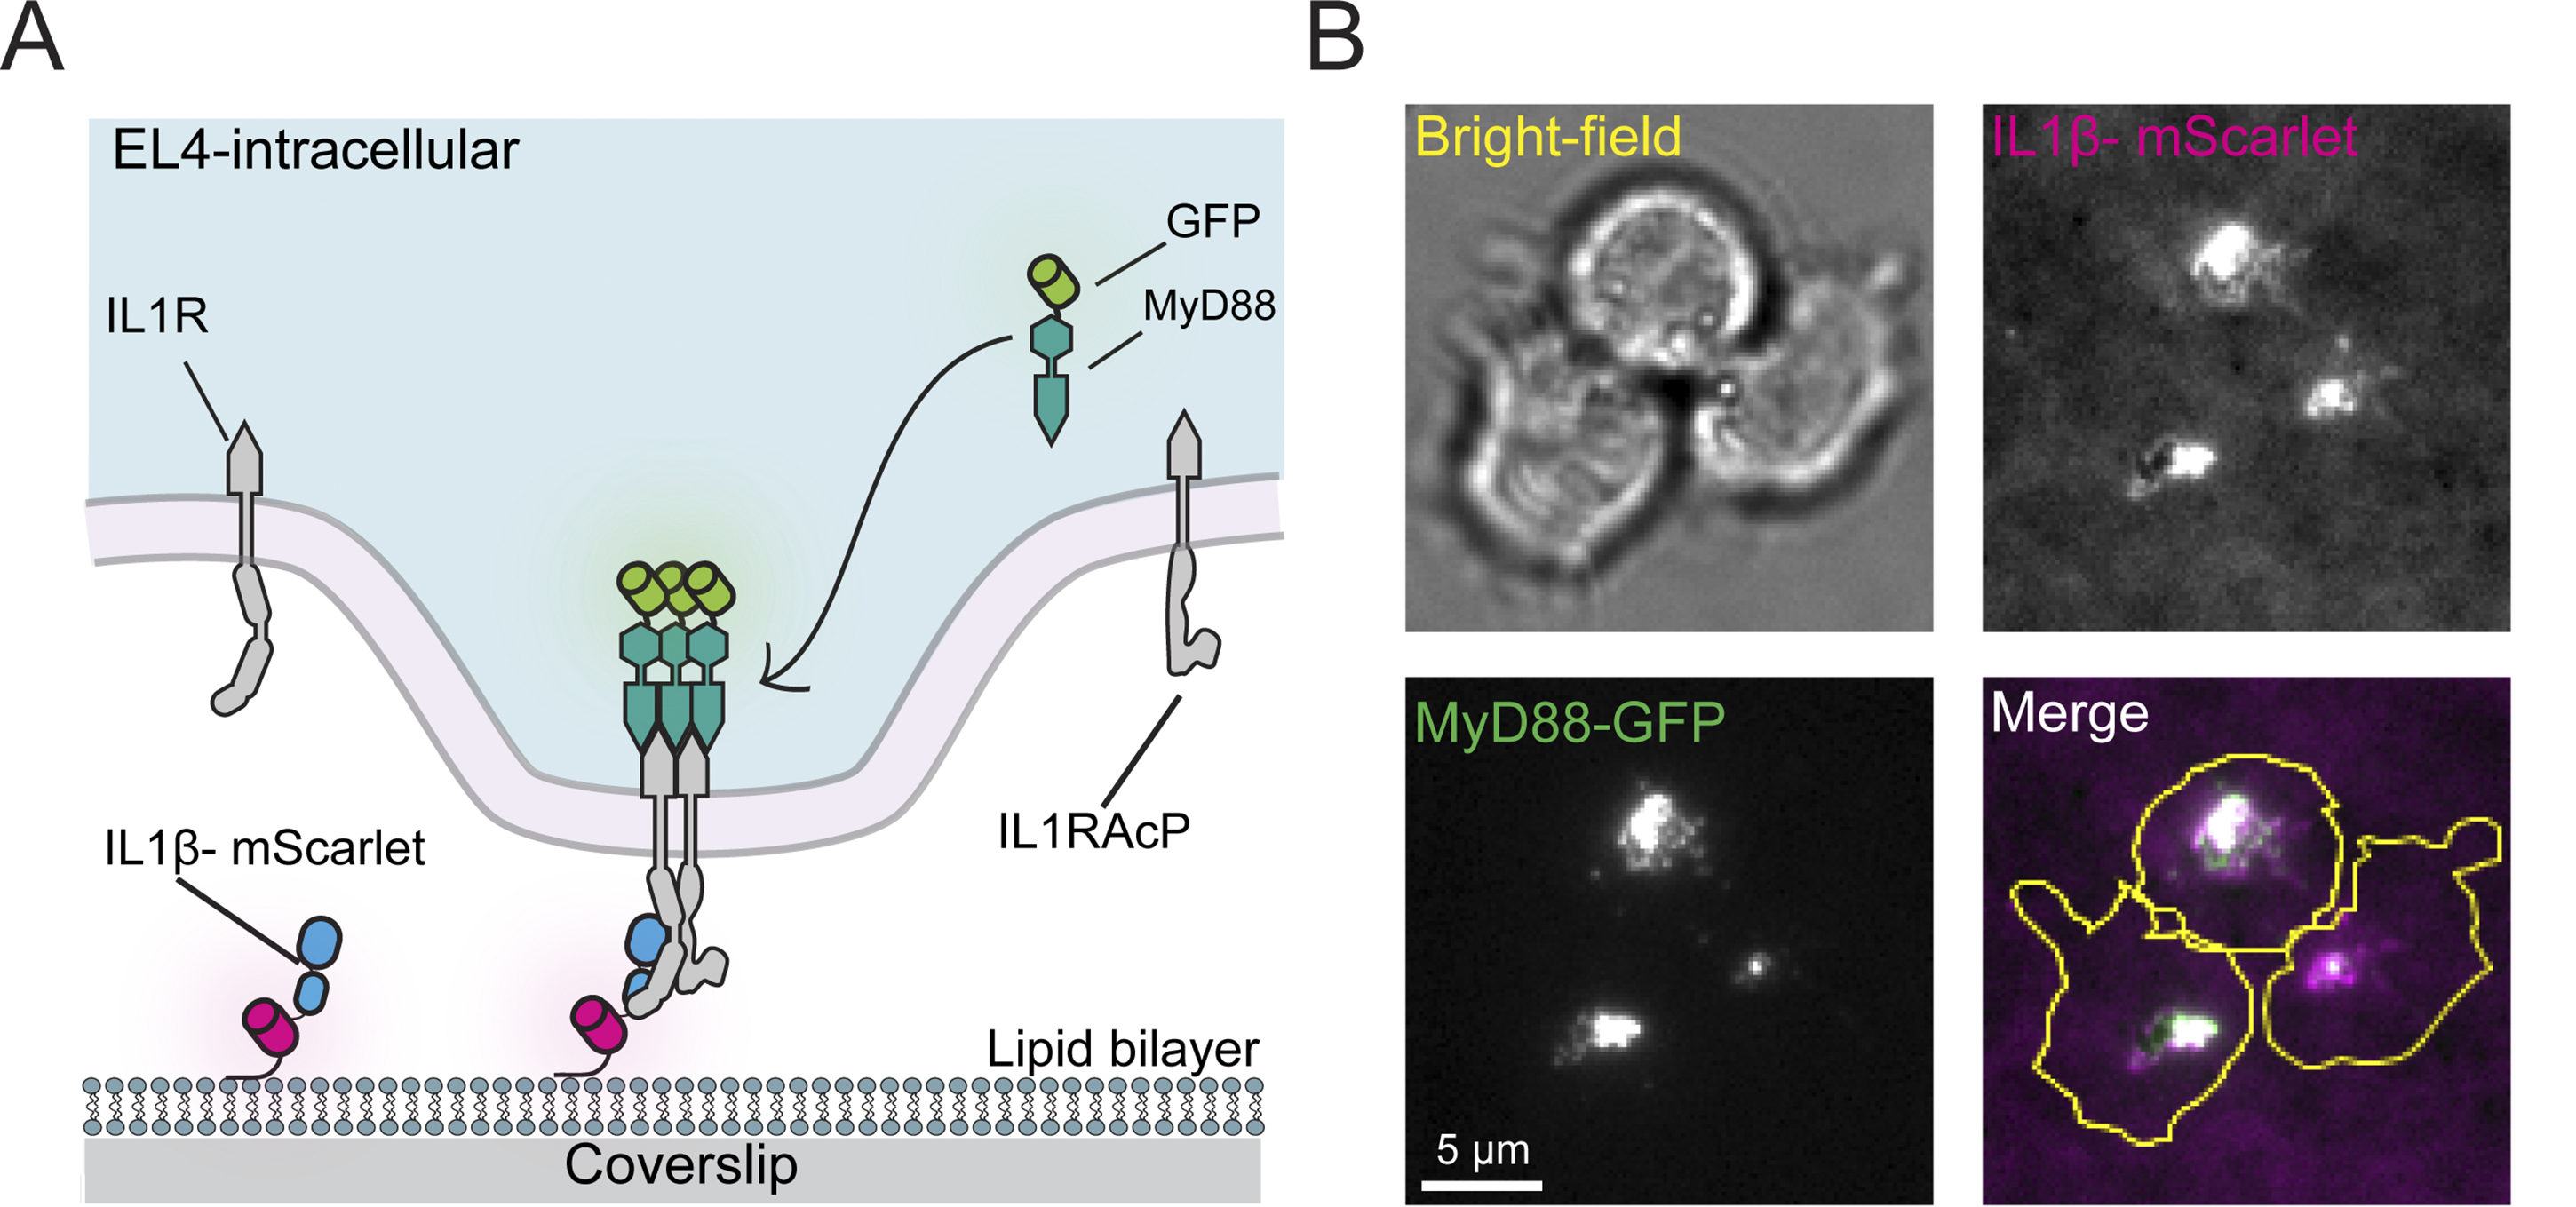
\includegraphics[width=\textwidth, height=\textheight, keepaspectratio]{jcb/fig1.png}}
\captionsetup{parbox=none}
\captionof{figure}[Membrane-tethered IL-1{\textbeta} triggers the relocalization of MyD88 to the cell surface.]{\textbf{Membrane-tethered IL-1{\textbeta} triggers the relocalization of MyD88 to the cell surface.}
\\
\\
(A) The schematic of a SLB functionalized with IL-1{\textbeta} labeled with mScarlet.
\\
\\
(B) TIRF and brightfield microscopy images of EL4 cells expressing MyD88-GFP after landing on a SLB functionalized with IL-1{\textbeta}-mScarlet puncta of IL-1{\textbeta}-mScarlet formed at the cell--SLB interface. MyD88-GFP was recruited to IL-1{\textbeta}-mScarlet puncta.
\\
\\
(Figure courtesy of Marcus Taylor. Figure, description adapted from \autocite{Deliz-Aguirre_2021}.)}
\label{p1:1}
\end{centering}

To validate that gene-edited cell lines expressed the correct fusion protein, and to ensure that these fusions did not perturb signal transduction, several controls were performed. Elke Ziska and Nichanok Auevechanickul verified correct insertion of the fluorescent protein in edited genomic loci using DNA sequencing. Elke Ziska confirmed the correct molecular weight of the fusion protein using western blot analysis.

Numerous reports show that fluorescent protein fusions may perturb signaling functions \autocite{Miyawaki_2003}\autocite{Haugh_2012}. To ensure this was not the case, we performed additional controls. EL4 cells are known to secrete IL-2 in response to IL-1 \autocite{Hoegen_1989}. Thus, Fenja Gerpott measured IL-2 release using ELISA. This bulk assay showed that tagging Myddosome proteins did not perturb IL-1 transcriptional responses.

As a final control, Fakun Cao stimulated wild-type and gene-edited EL4 cells using IL-1. Then, cells were fixed and stained with antibodies against the RelA subunit of NF-κB and phosphorylated MAPK p38. The nucleus was counter-stained with DAPI. The fixed cells were imaged using a 20\times objective and widefield microscopy (Fig.~\ref{p1:S2}A, C). I created a custom image analysis pipeline to analyze the images. It spanned from preprocessing to segmentation to statistical analysis of the images (see Methods~\ref{section:staining_pipeline}). The data was plotted as shown in Fig.~\ref{p1:S2}B, D. I found that there was no statistically significant difference between WT and labeled cell lines (Fig.~\ref{p1:S2}B, D, excluding KO).


\begin{centering}
\centering{\includegraphics[width=\textwidth, height=\textheight, keepaspectratio]{jcb/figs2.png}}
\captionsetup{parbox=none}
\captionof{figure}[Gene-edited EL4 cells reconstitute RelA nuclear translocation and MAPK p38 induction.]{\textbf{Gene-edited EL4 cells reconstitute RelA nuclear translocation and MAPK p38 induction.}
\\
\\
(A) RelA translocation to the nucleus in WT and gene-edited EL4 cells. EL4 cell lines (30 min after addition to IL1{\textbeta}-labeled SLBs) were fixed and stained for RelA (magenta); DAPI stained nuclei (blue). Scale bar, 50 µm.
\\
\\
(B) Quantification of RelA nucleus-to-cytoplasm staining ratio. Violin plots show the single-cell distribution RelA nucleus-to-cytoplasm staining ratio. Colored dots superimposed on violin plots correspond to the average value in the independent experiments (n = 3 or 4 experimental replicates per cell line; each replicate encompasses measurements from >2,000 cells. Bars represent mean $\pm$ Standard Error of the Mean (SEM). P-values were calculated using a two-tailed unpaired Student's t test.
\\
\\
(C) Phospho-p38 staining intensity in WT and gene-edited EL4 cells. EL4 cell lines (30 min after addition to IL1{\textbeta}-labeled SLBs) were fixed and stained for phospho-p38 (magenta); DAPI stained nuclei (blue). Scale bar, 50 µm.
\\
\\
(D) Quantification of phospho-p38 staining intensity. Violin plots show the single cell distribution phospho-p38 staining intensity. Colored dots superimposed on violin plots correspond to the average value in the independent experiments (n = 3 or 4 experimental replicates per cell line; each replicate encompasses measurements from >6,000 cells). Bars represent mean $\pm$ SEM. P-values were calculated using a two-tailed unpaired Student's t test.
\\
\\
(Images obtained by Fakun Cao. Panels A, C plotted by Fakun Cao. Panels B, D analyzed, plotted by the thesis author. Figure, description extracted from from \autocite{Deliz-Aguirre_2021}.)}
\label{p1:S2}
\end{centering}

\section{MyD88 puncta are highly dynamic}
\sectionmark{MyD88 is dynamic}
Latty et al. have shown that MyD88 puncta are highly dynamic in live cells, exhibiting considerable brightness variability \autocite{Latty_2018}. Building on their previous observations, we aimed to generate and visualize MyD88-eGFP cell lines (described in Deliz-Aguirre et al., 2020). My colleagues and I imaged them.

The generated cell lines exhibited highly dynamic puncta, successfully mirroring the existing literature. While there is a spectrum of different brightness levels and lifetimes, I identified two broad categories of puncta which are shown in Fig.~\ref{p1:3a}: (1) dim and short-lived (in red), and (2) bright and long-lived (in blue).

These two types of MyD88-eGFP puncta could have . To confirm this, I proceeded to quantify the images. Yet, at the time of the study (2019), TrackMate was one of the few easy-to-use tools available for quantifying puncta in live cells \autocite{Tinevez_2017}. However, it lacked important features, including background subtraction, cell segmentation, coordinate-based colocalization analysis. Thus, I developed a completely new image analysis to quantify the images with the aforementioned features. The pipeline steps are detailed in Methods~\ref{section:pipeline_v1} with a more thorough explanation in Methods~\ref{chapter:PIRATES_PARLEYS}. The brightness and lifetime of MyD88 puncta were thoroughly quantified.


\begin{centering}
\centering{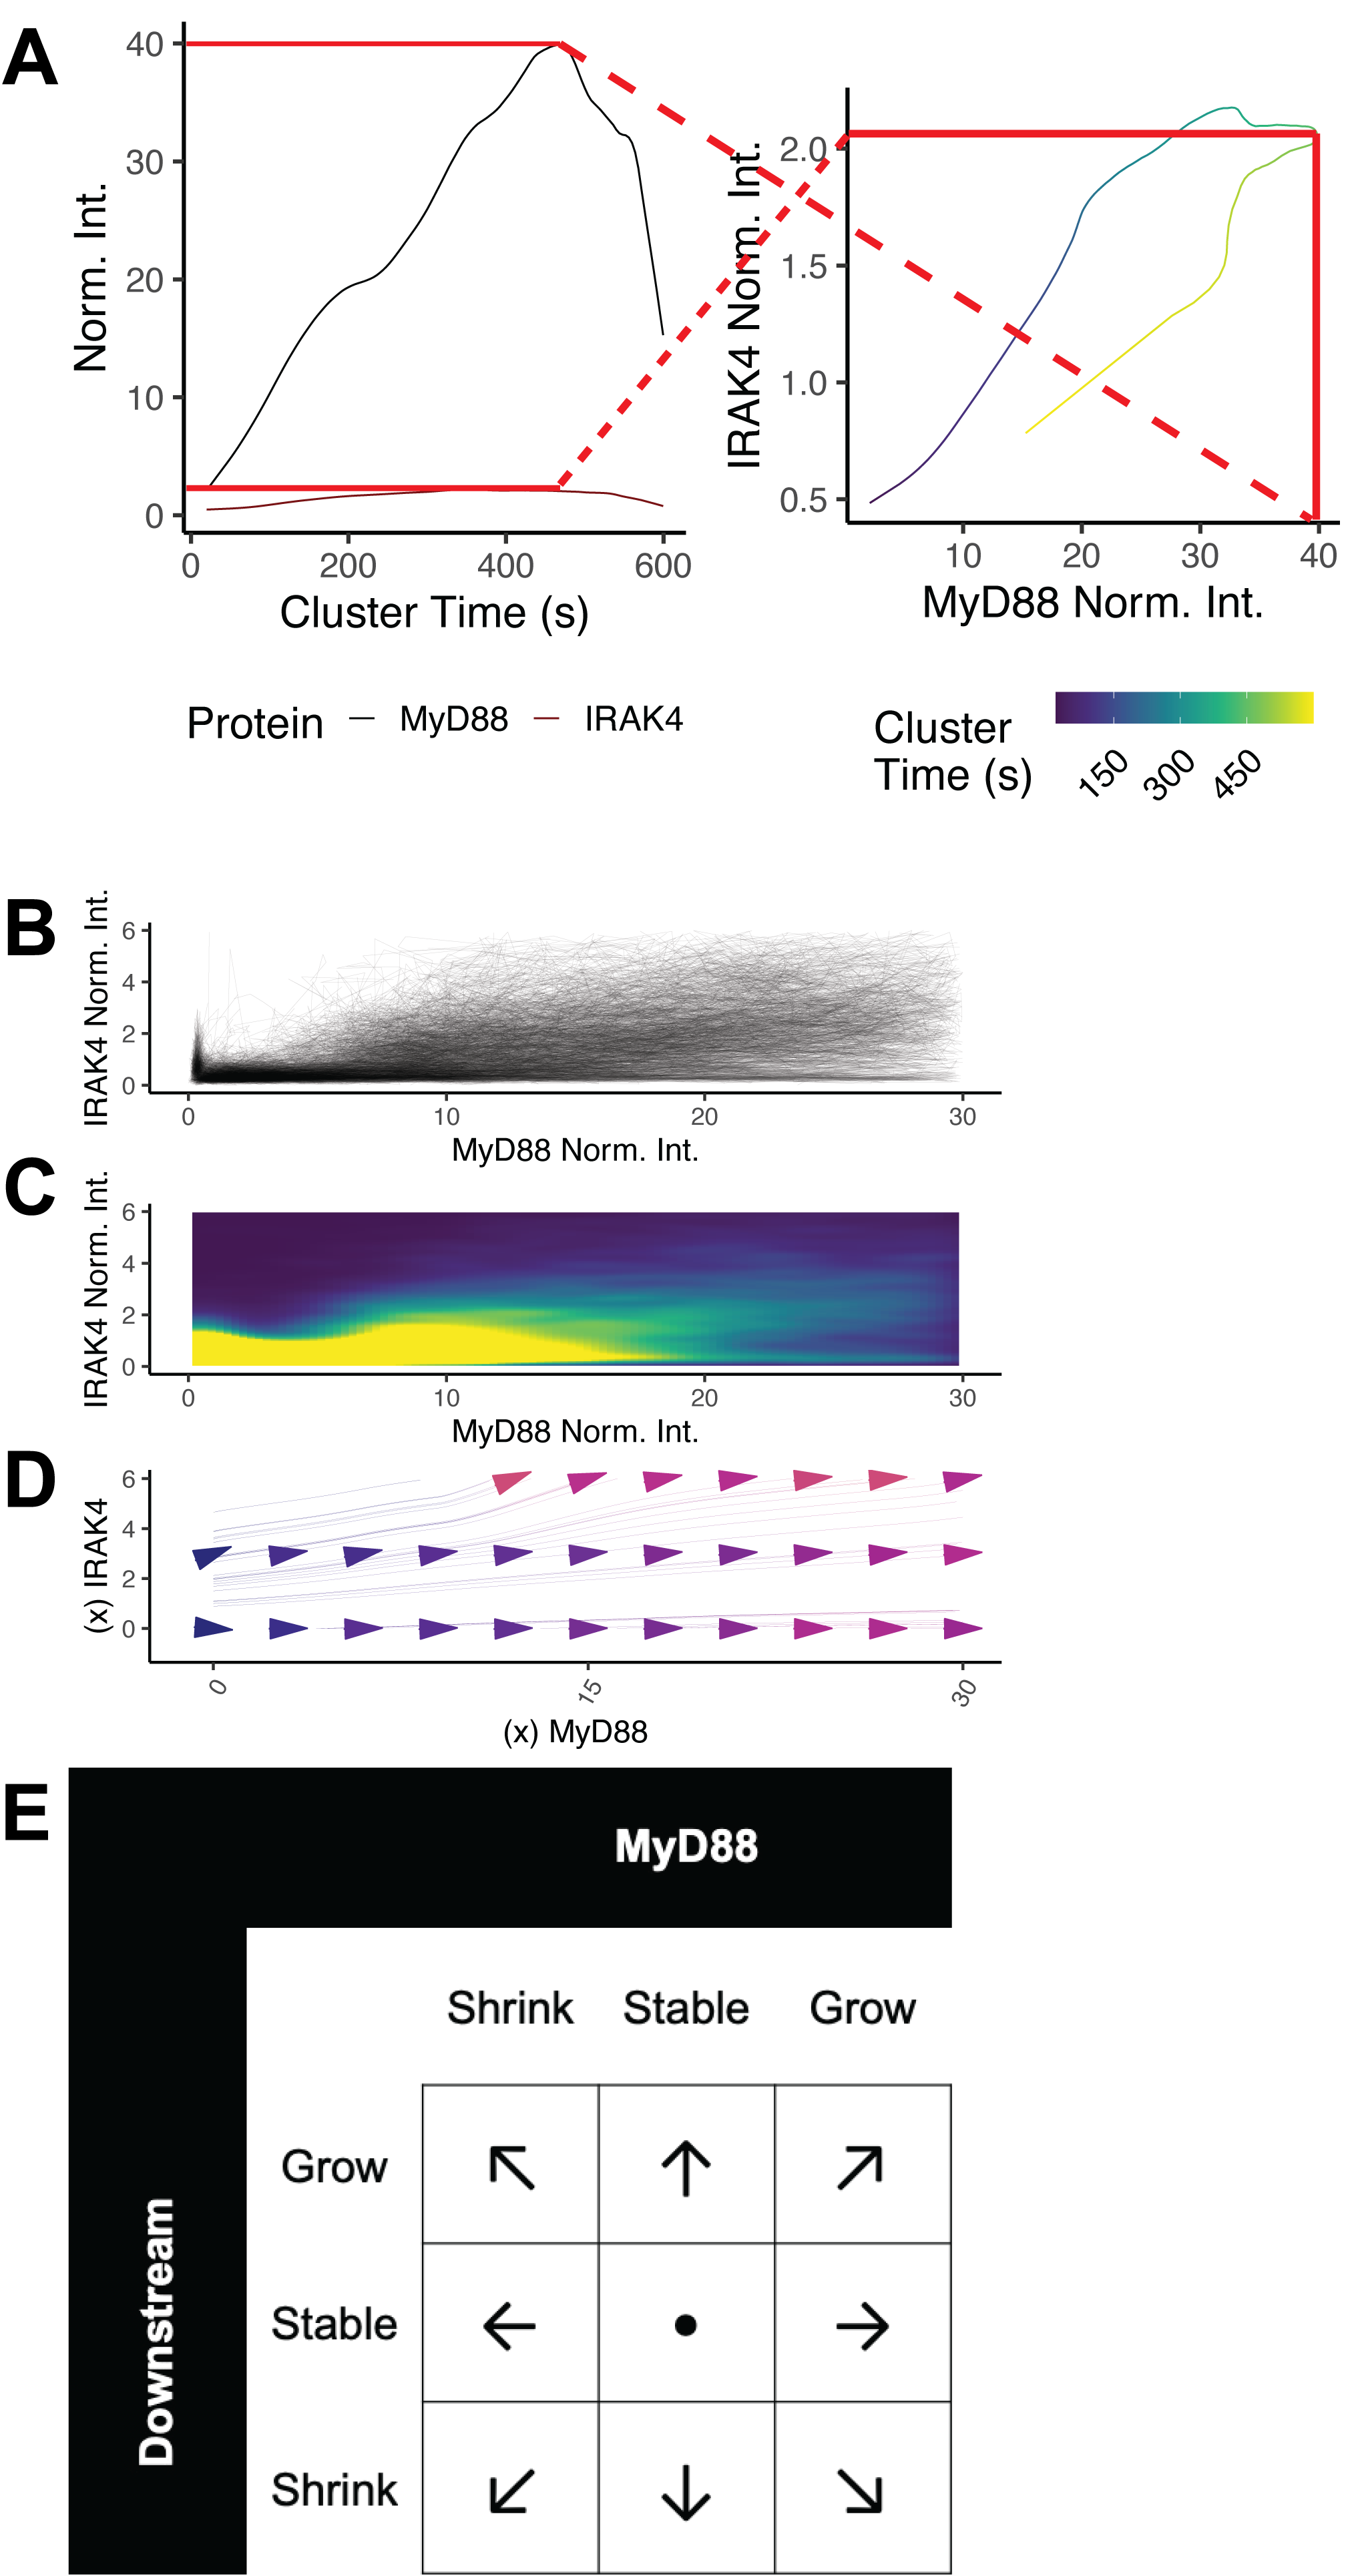
\includegraphics[width=\textwidth, height=\textheight, keepaspectratio]{jcb/fig3a.png}}
\captionsetup{parbox=none}
\captionof{figure}[MyD88-GFP puncta are heterogeneous]{\textbf{MyD88-GFP puncta are heterogeneous.} TIRF images of MyD88-GFP in an EL4 cell landing on an IL-1{\textbeta}-functionalized SLB. Overlaid colored boxes highlight examples of individual MyD88-GFP puncta. Red and orange ROI show the fluorescence intensity time series (left) and TIRF images (right) from Myddosomes that are short-lived (under 50 seconds) and dim (under 3\times GFP average intensity). Blue regions of interest show fluorescence intensity time series (bottom) and TIRF images (top) from two example MyD88-GFP puncta that grow in intensity and have a long lifetime (at least 50 seconds). The dashed gray lines on intensity plots mark the quantal MyD88-GFP fluorescence intensities, estimated from single GFP fluorophores. Calibration details in Methods.
\\
\\
(Imaging data courtesy of Fakun Cao. Image analysis, intensity plots done by the thesis author. Figure, descriptions extracted from \autocite{Deliz-Aguirre_2021}.)}
\label{p1:3a}
\end{centering}

I plotted the different max fluorescent intensities in the x-axis, and their frequency in the y-axis. As we can see in the dark blue curve in Fig.~\ref{p1:3b}A, MyD88 has a wide range of brightness levels. This shows that MyD88 puncta have heterogeneous sizes. However, this could mean that I am observing either (1) small MyD88 oligomers assembling, or (2) large MyD88 scaffolds as big as a Myddosome, coalescing to form super-Myddosomes \autocite{Latty_2018}. To establish which of the two models is correct, I needed to establish the stoichiometry using fluorescent intensities.

Using purified fluorophores in glass to determine protein stoichiometries from fluorescent brightness is an established technique \autocite{Latty_2018}\autocite{Douglass_2005}. Latty et al. used GFP dimers to estimate MyD88 stoichiometries from TIRF-M images. Similarly, I calculated the brightness of eGFP monomers using the same image analysis pipeline as before (see Methods~\ref{subsection:normalization}). The brightness of monomeric GFP puncta are shown in Fig.~\ref{p1:3b}A in the green curve.

Now that we can convert MyD88 brightness levels to MyD88 stoichiometries, my next step was to quantify the observed two puncta types, dim and bright, as shown in the Fig.~\ref{p1:3a} montages. Assembled Myddosome have 6\times MyD88 \autocite{Lin_2010}. Thus, now that I can compare TIRF-M images with structural studies, I proceeded to calculate the mean and standard deviation of the monomeric GFP to extrapolate how bright a 6\times MyD88-GFP complex would be. The estimated Gaussian curve of a 6\times MyD88 complex is shown in Fig.~\ref{p1:3b}A as a light blue curve. If I were to sort the MyD88 puncta using a 6\times GFP threshold, only 50\% of the Gaussian curve would be captured, which would represent only half of the assembled puncta. To capture $\approx 98\%$ of the 6\times MyD88-GFP curve, I adjusted the threshold to 4.5\times GFP (Fig.~\ref{p1:3b}A in the shaded box).\footnote{Technical replicates in Fig.~\ref{p1:S3}A} One limitation of this approach is that some smaller assemblies would be included in the analysis.

Revisiting the MyD88 line shown in dark blue in Fig.~\ref{p1:3b}A, the normalization suggests that most MyD88 assemblies are small. To confirm, I categorized the puncta as dim (under 4.5\times MyD88, red) or bright (at least 4.5\times MyD88), as shown in the x-axis of Fig.~\ref{p1:3b}B. Then, I calculated the percent of MyD88 puncta that meets the criteria, as shown in the y-axis of Fig.~\ref{p1:3b}B.\footnote{Technical replicates in Fig.~\ref{p1:S3}B} The evidence shows that most puncta are dim and have under 4.5\times MyD88.

Having observed that dim puncta were short-lived and that bright puncta were long-lived (sample puncta shown in Fig.~\ref{p1:3a}), I hypothesize that the dim puncta are transient MyD88 oligomers, while brighter puncta represent stable and fully-assembled Myddosomes. I proceed to quantify the lifetime of the puncta based on its brightness. I defined lifetime as how long the MyD88 puncta persists for. Using the pipeline data, I plotted a histogram with lifetime in the x-axis, and the puncta count in the y-axis (Fig.~\ref{p1:3b}C). Because most events were small, I adjusted the y-axis to log-scale,\footnote{More specifically, $\log(x+1)$ to account for zero counts} so that the less frequent long-lived events can be visualized. Fig.~\ref{p1:3b}C shows that dim events dominate the short lifetimes because the red bar (dim events) is taller than the blue bar (bright events).\footnote{Technical replicates in Fig.~\ref{p1:S3}C} However, after 50 seconds, the blue bar is taller than the red bar, which means that long-lived events are mainly bright. To validate these findings, I calculated the percentage of bright events (at least 4.5\times MyD88) in both short-lived (less than 50 seconds) and long-lived (at least 50 seconds) puncta. The analysis showed that 8\% of short-lived events have at least 4.5\times MyD88 while 69\% of long-lived events have at least 4.5\times MyD88 (Fig.~\ref{p1:3b}D).\footnote{Technical replicates in Fig.~\ref{p1:S3}D}

These findings show that MyD88 puncta are highly dynamic, having a gradation of oligomer lengths and lifetimes (Fig.~\ref{p1:3b}B and C, respectively). Most MyD88 puncta were dim and short-lived (Fig.~\ref{p1:3b}C). At the same time, brighter puncta live longer (Fig.~\ref{p1:3b}D). Next, I will explore the process that generates MyD88 heterogeneity.


\begin{centering}
\centering{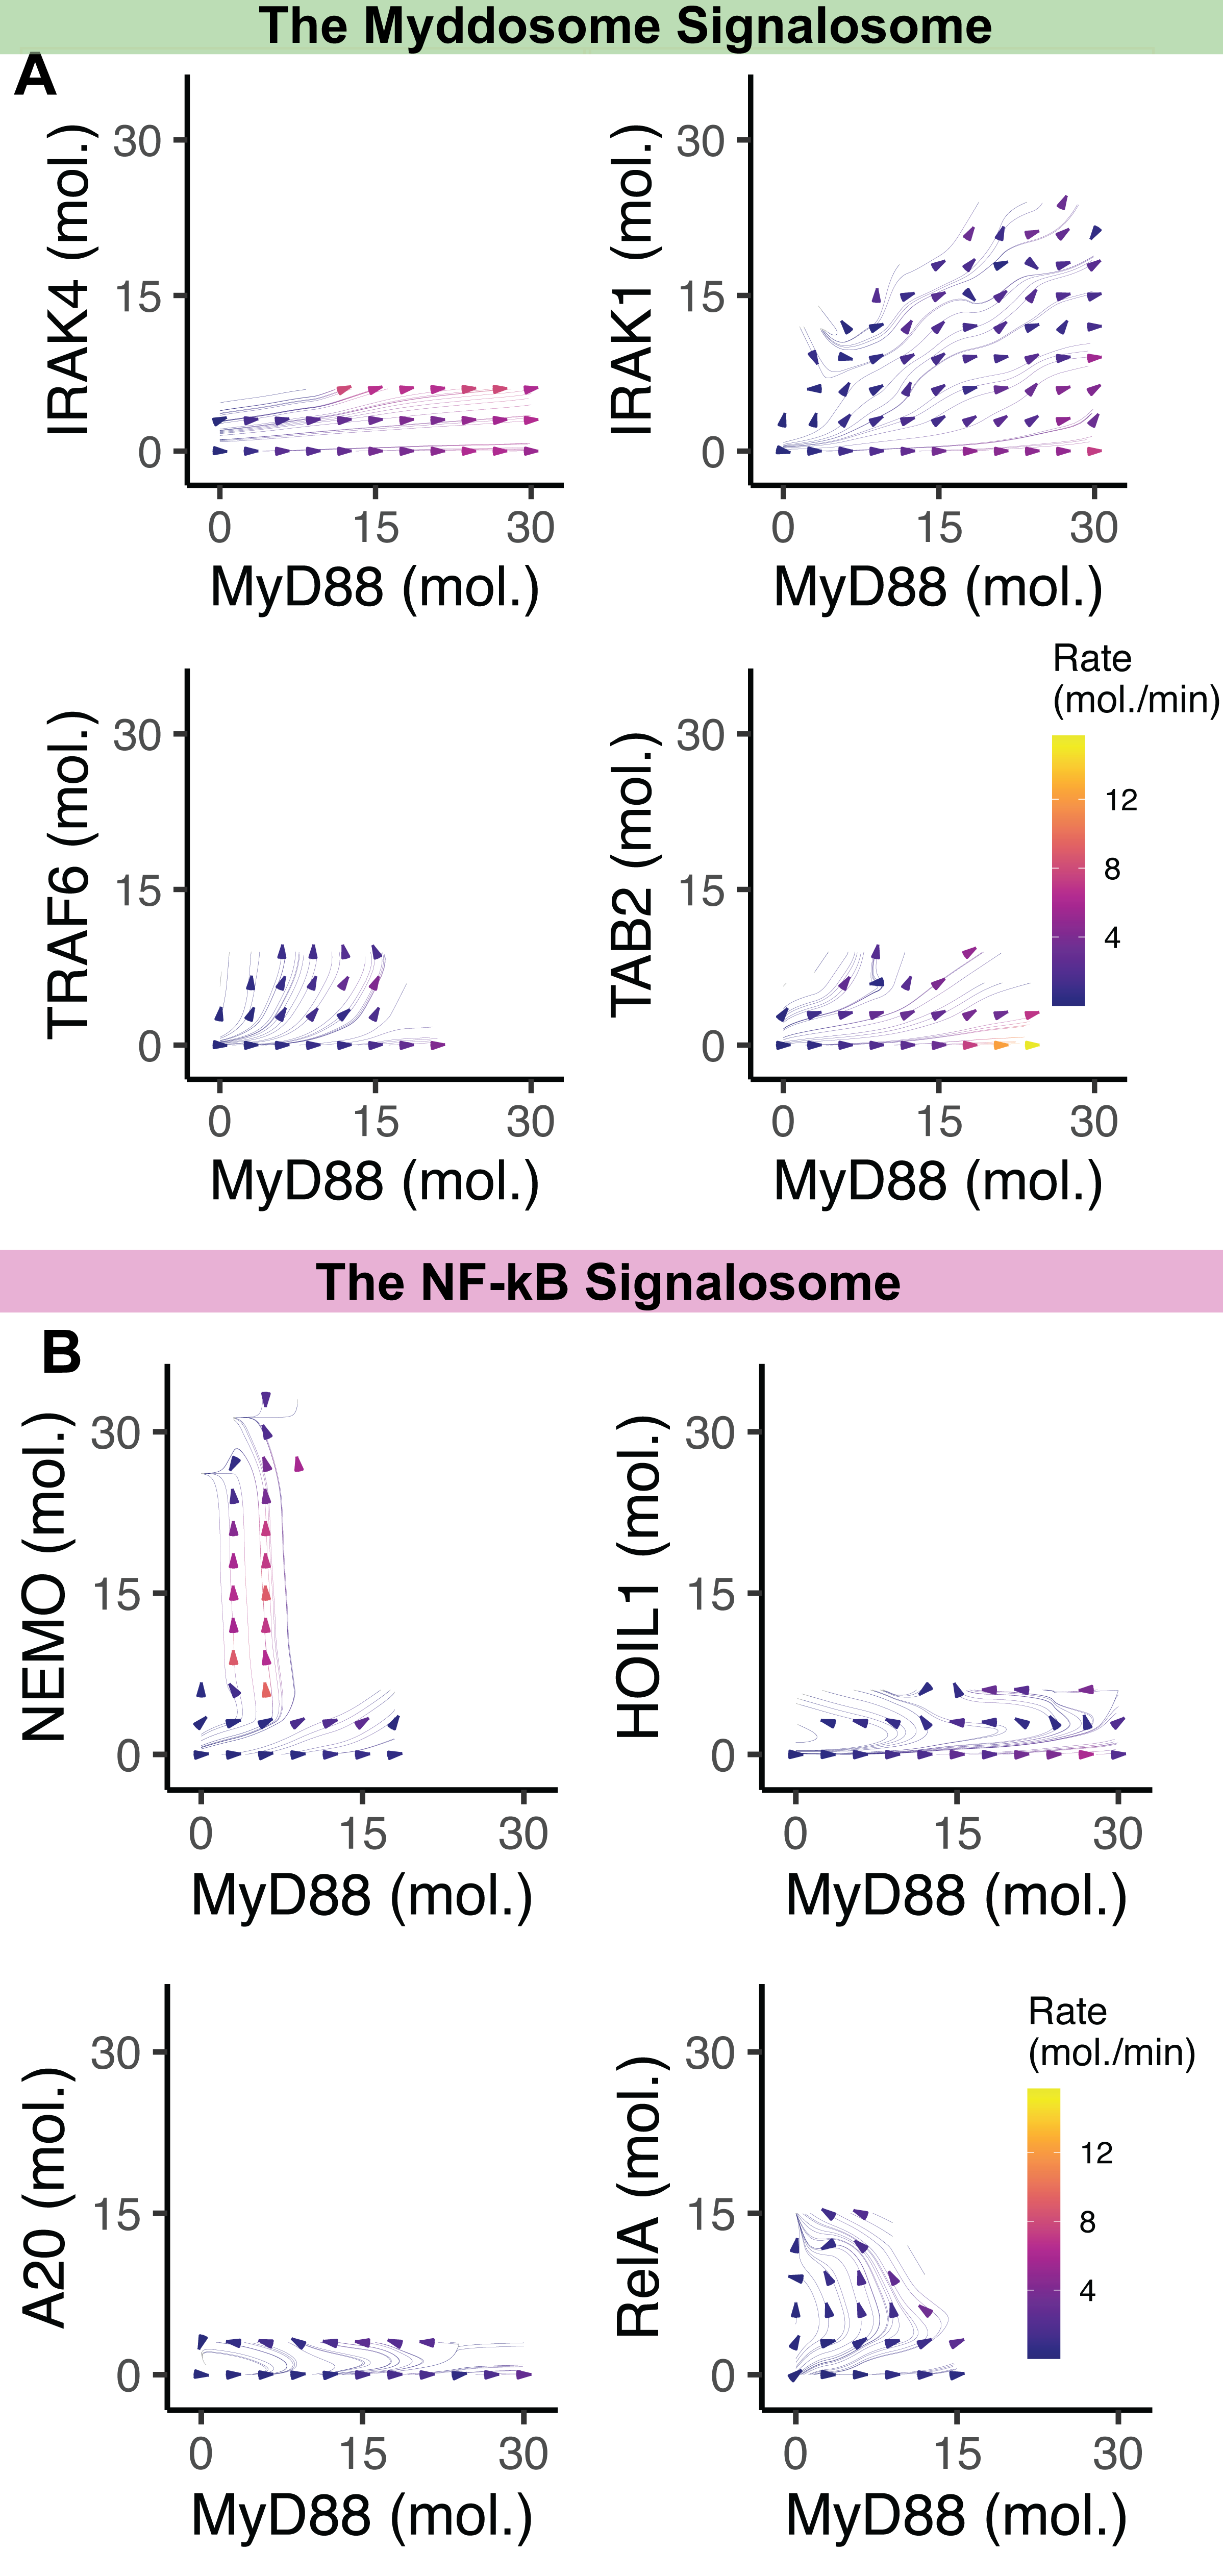
\includegraphics[width=\textwidth, height=\textheight, keepaspectratio]{jcb/fig3b.png}}
\captionsetup{parbox=none}
\captionof{figure}[Bright MyD88-GFP puncta have longer lifetimes]{\textbf{Bright MyD88-GFP puncta have longer lifetimes.}
\\
\\
(A) Density plot of the maximum fluorescent intensity of MyD88-GFP puncta (dark blue, n = 2,422 tracked MyD88-GFP particles from 14 cells) compared with single molecules of GFP (green, n = 397 GFP particles) and estimated intensity distribution of a 6\times GFP multimer (light blue). Shaded blue region designates intensity values >4.5\times GFP.
\\
\\
(B) Quantification of the proportion (\%) of MyD88-GFP puncta per cell that have a maximum fluorescence intensity under 4.5\times GFP or at least 4.5\times GFP. Violin plots show the distribution of the cell data. Data points superimposed on violin plots are the averages of independent experiments. Bars represent mean $\pm$ SEM (n = 6 experimental replicates, with 6--24 cells measured per replicate).
\\
\\
(C) Distribution of MyD88-GFP puncta lifetimes. Myddosomes were classified by maximum fluorescence intensity under 4.5\times or at least 4.5\times GFP (n = 2,037 under 4.5\times GFP versus n = 385 at least 4.5\times GFP tracked MyD88-GFP puncta combined from 14 cells). Scale is $\log(x+1)$.
\\
\\
(D) Quantification of the proportion (\%) per cell of MyD88-GFP puncta with an intensity maximum at least 4.5\times GFP categorized by lifetimes under 50 seconds or at least 50 seconds. Violin plots show the distribution of the cell data. Data points superimposed on the violin plots are the averages from independent experiments. Bars represent mean $\pm$ SEM (n = 6 experimental replicates, with 6--24 cells measured per replicate).
\\
\\
(A-D: Images acquired by Fakun Cao and the thesis author, and analyzed, plotted by the thesis author. Figure, descriptions extracted from \autocite{Deliz-Aguirre_2021}.)}
\label{p1:3b}
\end{centering}

As discussed in the Introduction~\ref{section:intro_Myddosome}, the MyD88 oligomerization mechanism has not been established, with two models put forward: preassembled oligomers and ligand-induced oligomerization. The detection of small MyD88 assemblies (Fig.~\ref{p1:3b}) suggest ligand-induced oligomerization. Should the ligand-induced oligomerization model be correct, then the intermediate events are MyD88 oligomers attempting to assemble full Myddosomes. This process should be gradual. Should the pre-assembled scaffold model be correct, then the Myddosome assembly should have large steps.

For each punctum, I calculated its lifetime as before and plotted it in the x-axis. To determine its growth, I calculated the maximum size minus the starting size. I call this the change (∆) in intensity, and plotted it in the y-axis. Fig.~\ref{p1:3c}A shows an example punctum, and how these parameters were calculated.  Should assembly be ligand-induced, then most events should have little to no growth. This would mean that a scatterplot would show overplotting at the origin. To avoid this scenario, I opted for a 2D density plot which would enable me to visualize the frequency of events at the intersection of lifetime and growth. In color is the frequency of events in log scale, with darker shades indicating more frequent events (Fig.~\ref{p1:3c}B). As we can see in Fig.~\ref{p1:3c}B,\footnote{Technical replicates in Fig.~\ref{p1:S3}E}  the darkest region is near the origin, meaning that most puncta did not grow and had short lifetimes.We can also see that the longer the lifetime, the more the change in intensity, gradually. As an aid to intuition, I added a trendline and calculated the correlation coefficient between lifetime and change in intensity.  This revealed a moderately-strong correlation (R = 0.59, Spearman’s rank correlation coefficient), suggesting that longer-lived puncta were more likely to increase in size.

Because MyD88 growth was gradual, slowly growing from small to larger assemblies, and because lifetime and change in intensity were correlated, I conclude that MyD88 oligomerization is ligand-induced. Because assemblies were forming \emph{de novo}, the heterogeneity in lengths could represent different stopping points before the Myddosome assembly aborted. To confirm that long MyD88 oligomers are the ones signaling, we titrated the ligand.


\begin{centering}
\centering{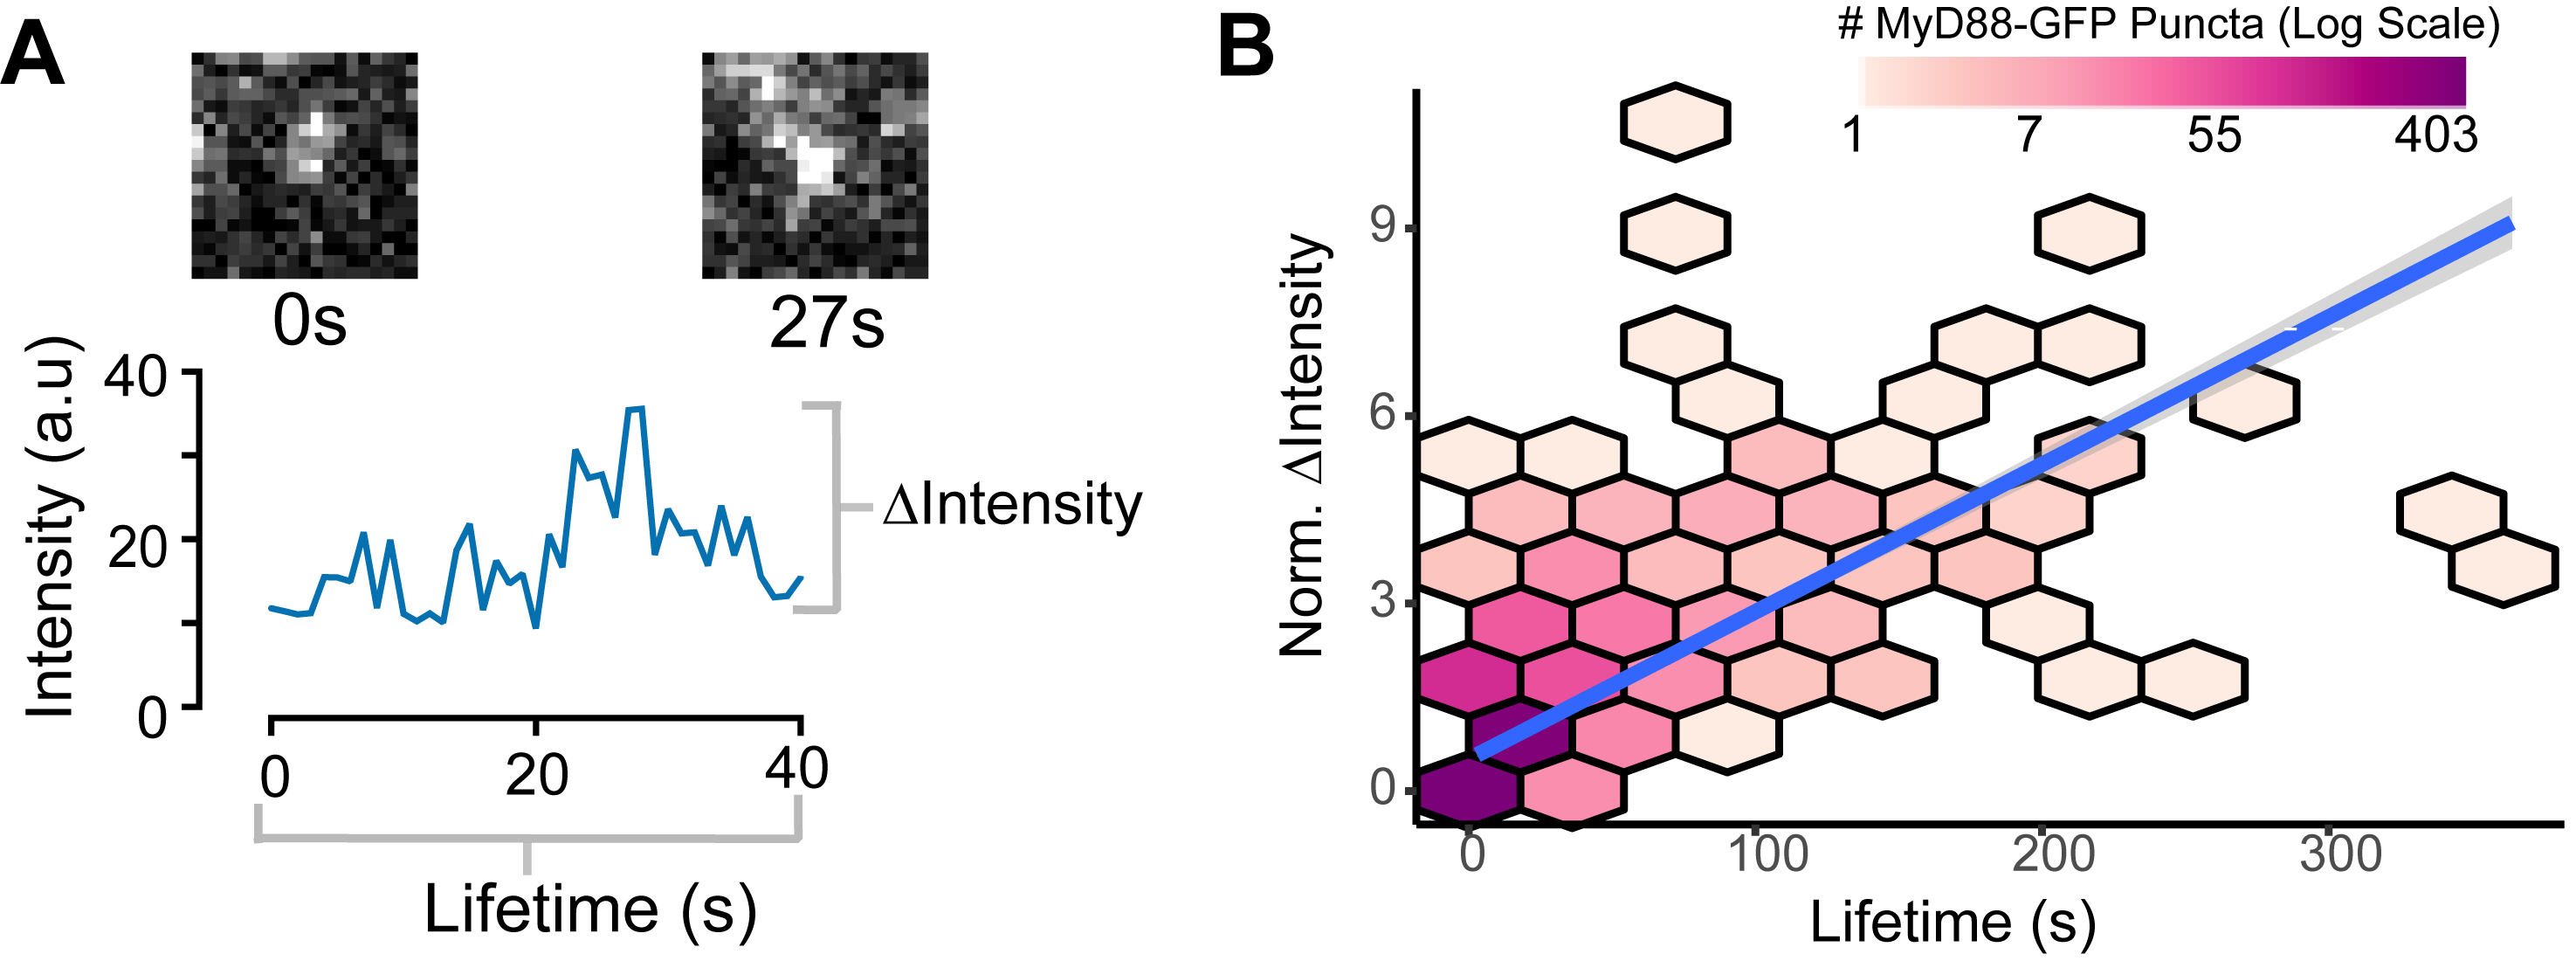
\includegraphics[width=\textwidth, height=\textheight, keepaspectratio]{jcb/fig3c.png}}
\captionsetup{parbox=none}
\captionof{figure}[MyD88-GFP puncta grows over time]{\textbf{MyD88-GFP puncta grows over time.} Correlation between growth in intensity and lifetime of MyD88-GFP puncta.
\\
\\
(A) TIRF images and intensity trace of a MyD88-GFP puncta. The change in intensity calculated as maximum intensity subtracted by the initial intensity.
\\
\\
(B) 2D histogram of MyD88-GFP puncta lifetime versus changed in fluorescent intensity. Linear fit is shown as a blue line with the 95\% CI shown in gray (Spearman’s rank correlation coefficient R = 0.59, P < 0.001, n = 1,763 MyD88 tracks, combined from 14 cells).
\\
\\
(A) Panel courtesy of Marcus Taylor using images acquired by Fakun Cao and the thesis author. B: Images acquired by Fakun Cao and the thesis author. Analysis, plots by the thesis author. Figure, descriptions extracted from \autocite{Deliz-Aguirre_2021}.)}
\label{p1:3c}
\end{centering}

Latty et al. showed that the amount of LPS (TLR4 ligand) functions to the size of MyD88 assemblies \autocite{Latty_2018}. Similarly, I tested how the IL-1 ligand leads to MyD88-mediated signaling. Having observed diverse assembly sizes, and that only a small fraction were large MyD88 assemblies, I reasoned that large MyD88 signals, and that short MyD88 oligomers do not. To test the hypothesis, Fakun Cao stained cells with phospho-p38 (MAPK activation marker), and I analyzed the data. By applying various ligand densities via SLB, we were able to control IL-1\textbeta stimulation strength. Previously (Figs.~\ref{p1:3a}-~\ref{p1:3c}), we used 32 molecules µm\textsuperscript{-2}. Here, we used no ligand (negative control), low ligand (0.1 mol. µm\textsuperscript{-2}), and high ligand densities (320 mol. µm\textsuperscript{-2}). 

The visual inspection of the low ligand density regimen in p-p38 stained cells showed no signal (black images) for the p-p38 channel and signal (blue light) for the DAPI channel (Fig.~\ref{p1:3d}A, montage). This means that no ligand and low ligand are equivalent (p = 0.17, n.s.), with no MAPK activation (Fig.~\ref{p1:3d}A, violin plots). The positive control (DAPI) showed cells were present in the field of view. In contrast, the high ligand density cells had a p-p38 signal (positive stain), indicating that a high ligand density leads to signaling (Fig.~\ref{p1:3d}A, montage). The violin plots inFig.~\ref{p1:3d}A showed that low and high ligand density had different responses (p = 0.037).

Similarly, I tested the proportion of large MyD88 puncta in low and high ligand density (Fig.~\ref{p1:3d}B). The data showed that low ligand density had few MyD88 assemblies larger than 4.5\times MyD88 (Fig.~\ref{p1:3d}B, left). In contrast, the high ligand density led to the formation of larger MyD88 assemblies (Fig.~\ref{p1:3d}B, right).


\begin{centering}
\centering{\includegraphics[width=\textwidth, height=\textheight, keepaspectratio]{jcb/fig3d.png}}
\captionsetup{parbox=none}
\captionof{figure}[MyD88-GFP puncta are inducible]{\textbf{MyD88-GFP puncta are inducible.}
\\
\\
(A) Activation of phospho-p38 at different IL-1 ligand densities on SLBs. Left: Phospho-p38 staining on SLB labeled with 0.1 and 300 IL-1{\textbeta} per square micrometer. EL4 cell lines (30 min after addition to IL-1{\textbeta}-labeled SLBs) were fixed and stained for phospho-p38 (magenta); DAPI stained nuclei (blue). Right: Quantification of phospho-p38 staining. Violin plots show the single-cell distribution of staining intensities. Data points superimposed on the violin plots are the averages from independent experiments (n = 3 experimental replicates, with >6,000 cells measured per replicate). Bars represent mean $\pm$ SEM. P values were calculated using a two-tailed unpaired Student's t test.
\\
\\
(B) Quantification of the number of MyD88-GFP puncta per cell that assemble with intensity maxima at least 4.5\times GFP on SLB labeled with high and low IL-1 densities. Violin plots show the single-cell distribution of the total number of MyD88-GFP puncta per cell and those with lifetimes under 50 seconds or at least 50 seconds. Data points superimposed on the violin plots are the averages from independent experiments. Bars represent mean $\pm$ SEM (n = 3 experimental replicates, with 6--24 cells measured per replicate). P values were calculated using an unpaired Student's t test. fluo., fluorescence; Max, maximum; Norm., normalized.
\\
\\
(A: Panel courtesy of Fakun Cao. B: Imaging data courtesy of Fakun Cao. Image analysis, intensity plots done by the thesis author. Figure, descriptions extracted from \autocite{Deliz-Aguirre_2021}.)}
\label{p1:3d}
\end{centering}

These trends support the literature \autocite{Latty_2018} and my initial hypothesis that large, long-lived MyD88 assemblies are more adept at yielding an immune response. The results showed that a higher proportion of large MyD88 assemblies were associated with greater MAPK activation. More broadly, these observations point to a functional role for MyD88 oligomer length in modulating immune responses. An implication of these observations would be that larger MyD88 assemblies should recruit more IRAK4/1. Therefore, we imaged Myd88 and IRAK4 or IRAK1 next.

\section{Larger and kinetically stable MyD88 oligomers recruit IRAK4, IRAK1 sequentially}
\sectionmark{IRAK4/1 recruitment}
\label{section:IRAK_recruitment}
\sectionmark{IRAK4/1 recruitment}
Because I observed ligand-induced oligomerization, and because I also saw that larger MyD88 assemblies are associated with MAPK activation, I reasoned that large MyD88 oligomers, rather than smaller ones, are more effective at recruiting IRAK4 and IRAK1, two proteins downstream of MyD88 \autocite{Lin_2010}. To test this hypothesis, Elke Ziska and Nichanok Auevechanichkul generated two more cell lines: (1) MyD88-eGFP IRAK4-mScarlet and (2) MyD88-eGFP IRAK1-mScarlet.

The TIRF-M images show that MyD88 (green) and IRAK4/1 (magenta) puncta colocalize (white) at the cell surface in response to IL-1\textbeta stimulation (Fig.~\ref{p1:4a}A). As the sample montages illustrate (Fig.~\ref{p1:4a}B), there is temporal organization as MyD88 puncta appears first, then IRAK4 and IRAK1 last. Additionally, the time traces show that IRAK4/1 recruitment happens after MyD88 grows and becomes large (Fig.~\ref{p1:4a}C). To test these hypotheses, I wrote scripts to analyze the colocalization dynamics (see Methods~\ref{chapter:pipeline_v1}).


\begin{centering}
\centering{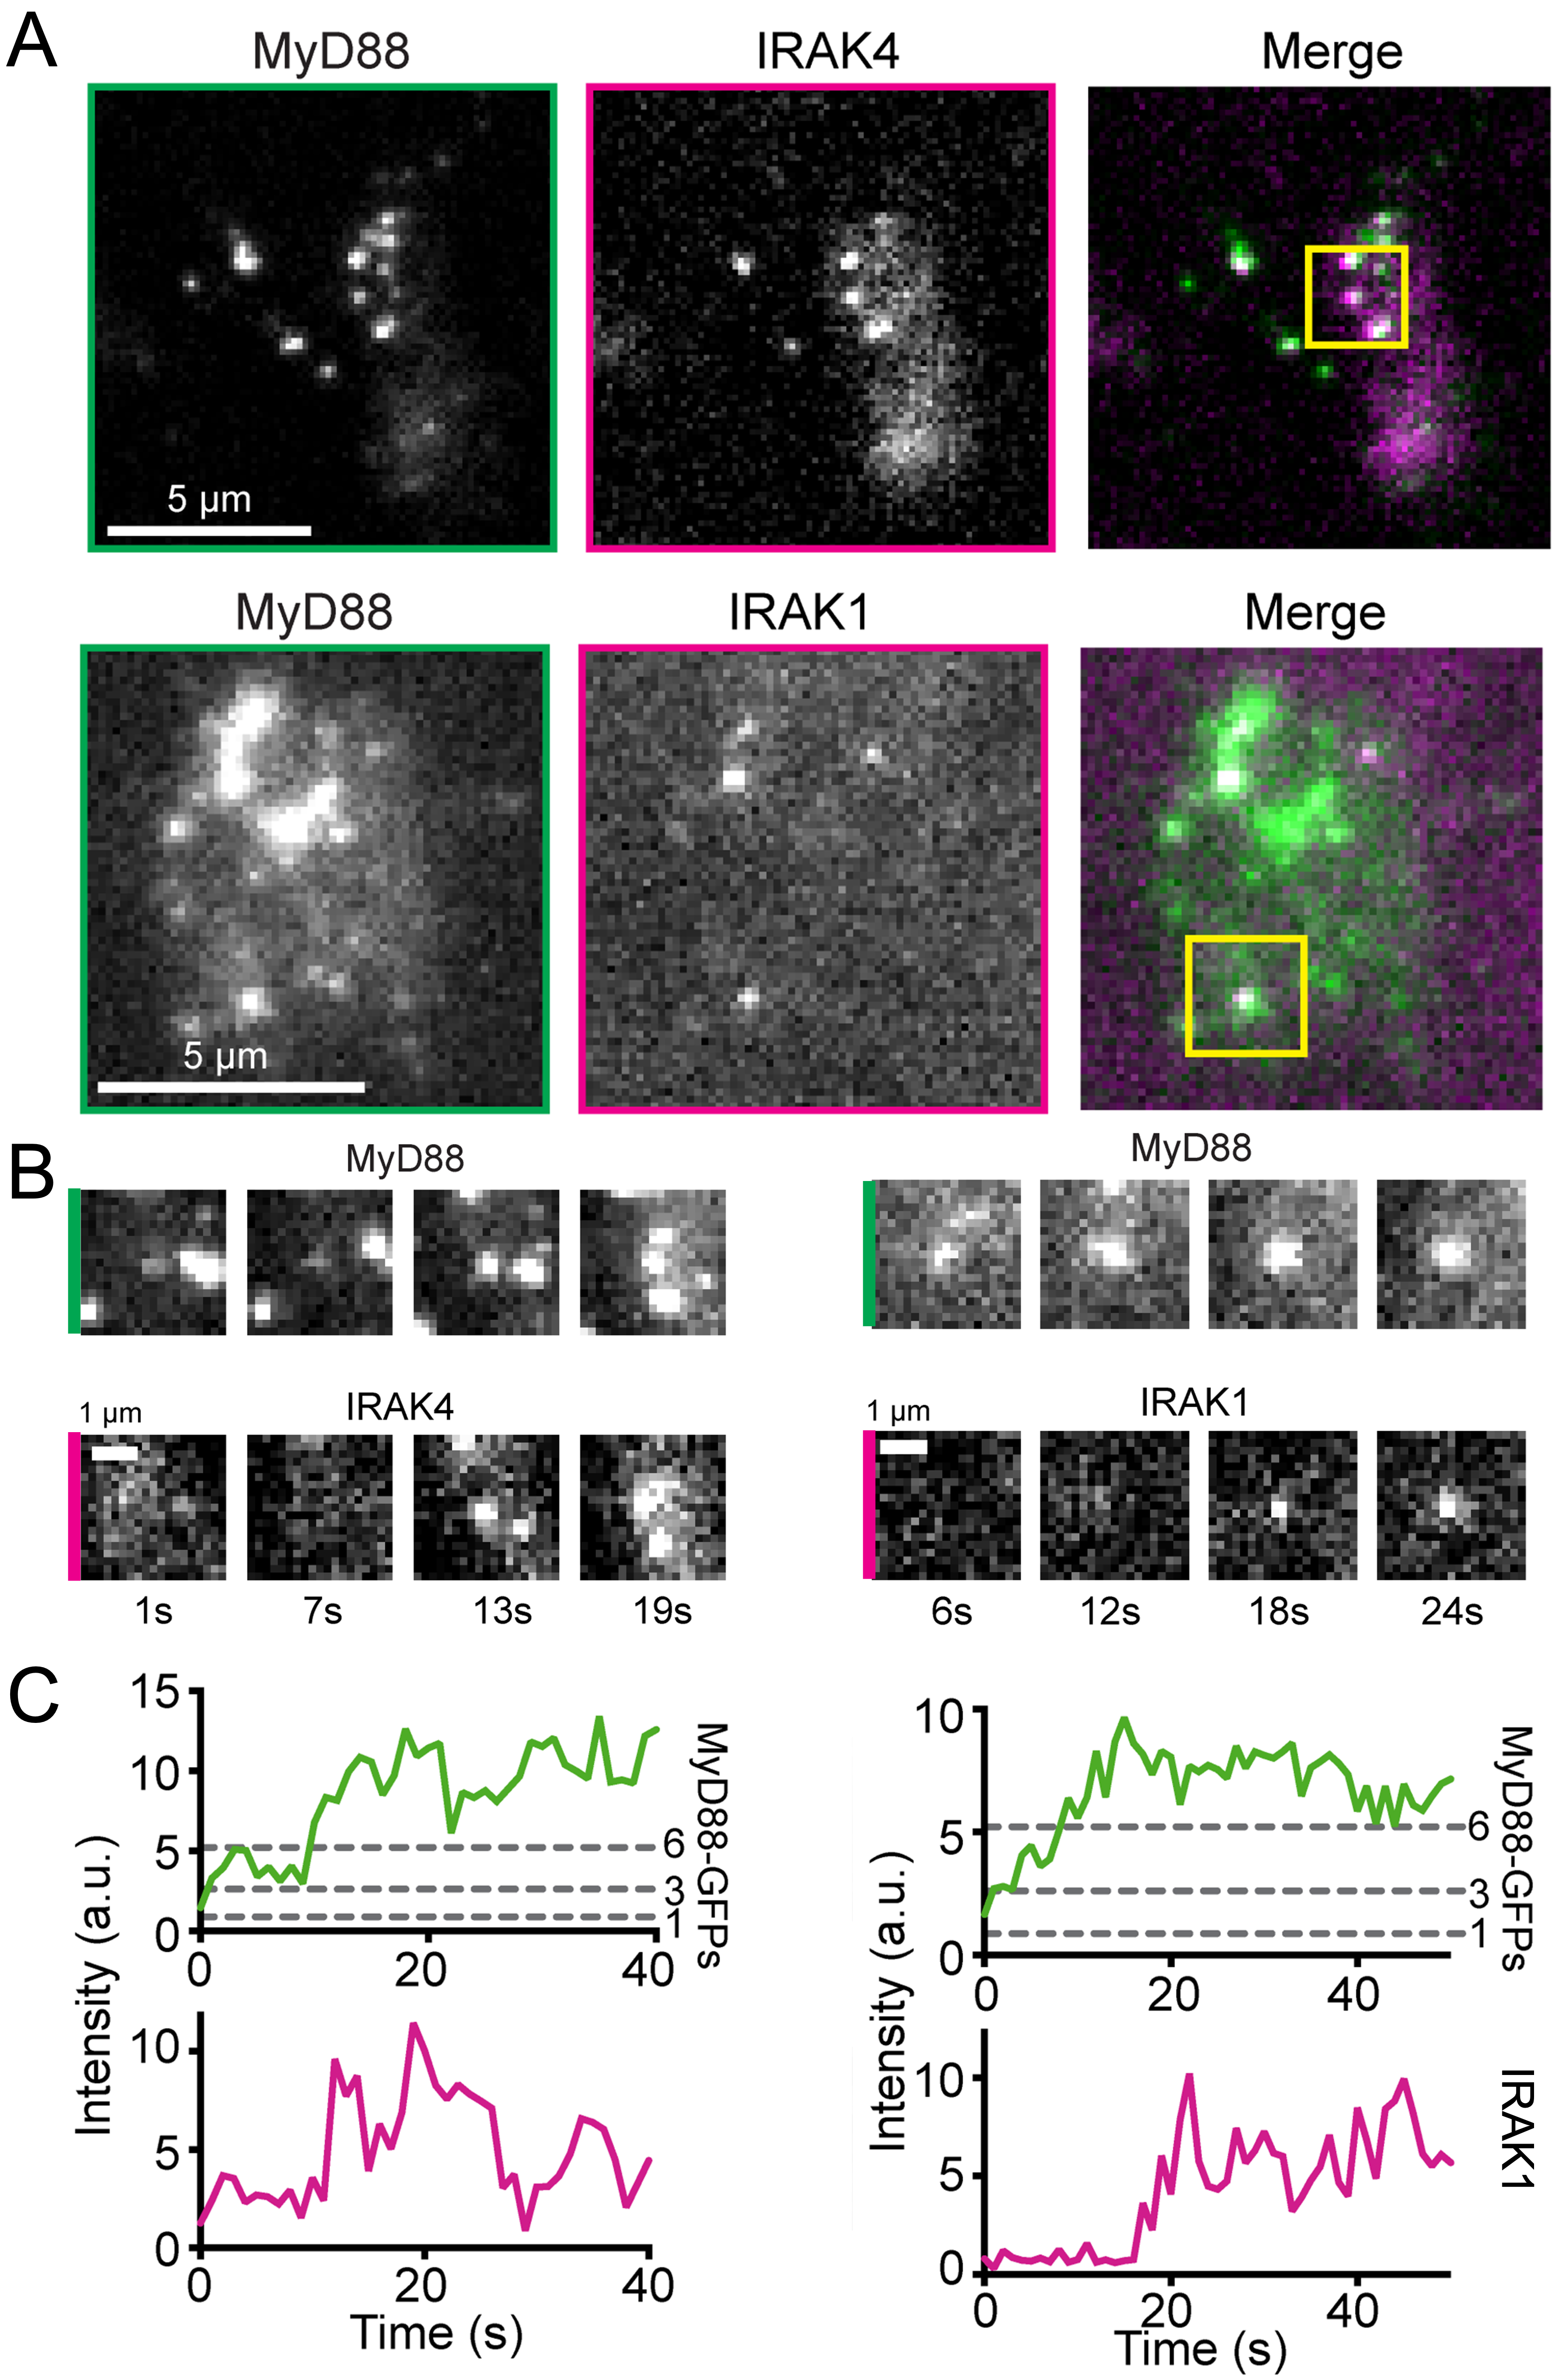
\includegraphics[width=0.75\textwidth, height=0.75\textheight, keepaspectratio]{jcb/fig4a.png}}
\captionsetup{parbox=none}
\captionof{figure}[IRAK4 and IRAK1 are recruited to MyD88]{\textbf{IRAK4 and IRAK1 are recruited to MyD88.}
\\
\\
(A)TIRF images of MyD88-GFP and (top) IRAK4-mScarletor (bottom) IRAK1-mScarlet.
\\
\\
(B). Region of interest (yellow box, merge image) shows an example of a MyD88-GFP spot colocalized with (left) IRAK4-mScarlet or (right) IRAK1-mScarlet.
\\
\\
(C) Timetraces of the TIRF images from the region of interest shown in B.
 and fluorescence intensity time series of MyD88-GFP and (left) IRAK4-mScarlet or (right) IRAK1-mScarlet. 
\\
\\
(Panels, imaging data courtesy of Marcus J. Taylor. Figure, descriptions extracted from \autocite{Deliz-Aguirre_2021}.)}
\label{p1:4a}
\end{centering}

I hypothesize that IRAK4 and IRAK1 are recruited to kinetically stable MyD88 puncta. To test this, I analyzed the lifetime and colocalization status of MyD88 puncta. I reasoned that kinetically stable MyD88 puncta would have longer lifetimes. Therefore, I categorized the MyD88 lifetimes as short-lived (under 50 seconds) and long-lived (at least 50 seconds), the same thresholds as before (Fig.~\ref{p1:3b}D). Then, I calculated the proportion of puncta that colocalized with IRAK4/1. In Fig.~\ref{p1:4b}A, we can see that only 3\% of MyD88 puncta colocalized with IRAK4 (black bar in “All”). Similarly, we can see that short-lived MyD88 puncta (less than 50 seconds) also have low colocalization with IRAK4 at a mere 1\% colocalization. Only when MyD88 persists for long-lived puncta (at least 50 seconds) do we see a stark difference at 32\% colocalization (Fig.~\ref{p1:4b}A).\footnote{Technical and biological replicates in Fig.~\ref{p1:S4}A} This was consistent across cell (violin plots) and image replicates (green dots). The IRAK1 data showed a similar trend. As we can see in Fig.~\ref{p1:4b}B, 5\% of MyD88 puncta colocalized with IRAK1. For short-lived MyD88 puncta, the colocalization with IRAK1 is lower at 3\%, and it jumps to 36\% in long-lived puncta (Fig.~\ref{p1:4b}B).\footnote{Technical and biological replicates in Fig.~\ref{p1:S4}C} This was consistent across cell (violin plots) and image replicates (orange dots), though with more variability than IRAK4. This establishes that IRAK4 and IRAK1 bind to kinetically stable MyD88 puncta. Having established in MyD88 that long-lived puncta and long oligomer length go hand-in-hand, I proceeded to quantify the oligomer length of MyD88 puncta that colocalized with IRAK4/1.

Structural studies have established that the Myddosome stoichiometry is 6-8\times MyD88, 4\times IRAK4 and 4\times IRAK1/2 \autocite{Lin_2010}\autocite{Moncrieffe_2020}. Based on this, I hypothesized that MyD88 oligomers must be long ($\geq$4.5\times) to recruit IRAK4/1. I drew density plots, and subset MyD88 puncta based on their colocalization status. IRAK4/1 positive MyD88 puncta were labeled as “+ve” and shaded green for IRAK4 or orange for IRAK1. IRAK4/1 negative MyD88 puncta were labeled as “-ve” and shaded white. As a visual aid, I added a dotted gray line at the 4.5\times MyD88 size threshold I have been using throughout this study. As we can see in Fig.~\ref{p1:4b}C-D, the IRAK4/1 negative white-shaded curves (-ve) have their peak and bulk of the curve to the left of the 4.5\times MyD88 gray line. The mean size of IRAK4-negative MyD88 was 3.2\times, and IRAK1-negative MyD88 was 3.7\times. This indicates that MyD88 puncta without IRAK4/1 colocalization are small and under 4.5\times MyD88. However, when we examine the IRAK4/1 colocalized data (+ve) in Fig.~\ref{p1:4b}C-D, we can see that the density curves shift to the right indicating that IRAK4/1-colocalized MyD88 are larger. 
 More specifically, the mean IRAK4-positive MyD88 was 11\times, and IRAK-1 positive MyD88 was 12\times.\footnote{Technical replicates in Fig.~\ref{p1:S4}B, D} I then drew violin plots of the percent of MyD88 puncta that colocalized IRAK4/1 using 4.5\times MyD88 as a size threshold. As we can see in the insert plot at Fig.~\ref{p1:4b}C-D, IRAK4/1 colocalized MyD88 are larger because the violin (cell replicate means) and dots (image replicate means) show a higher percentage in the y-axis (\% IRAK4/1 +ve Myddosomes per Cell”).

For the first time, MyD88-IRAK4 and MyD88-IRAK1 are visualized dynamically together in live cells. Consistent with the structural data \autocite{Lin_2010}\autocite{Moncrieffe_2020}, the data clearly shows that IRAK4/1 colocalizes with large MyD88 ($\geq$4.5\times) (Fig.~\ref{p1:4b}C). We add that these MyD88 puncta must be kinetically stable (long-lived) to colocalize with IRAK4 and IRAK1 (Fig.~\ref{p1:4b}A-B). Moreover, most MyD88 assemblies triggered by IL-1 stimulation do not recruit IRAK4/1 (Fig.~\ref{p1:4b}A-B, “All”), and like the staining data indicated (Fig.~\ref{p1:3d}), most MyD88 assemblies do not transduce signals due to their size. Therefore, IRAK4/1 have a flexible requisite MyD88 size before assembling. Next, I explored the temporal organization of assembly and asked what is the assembly sequence of the Myddosome.


\begin{centering}
\centering{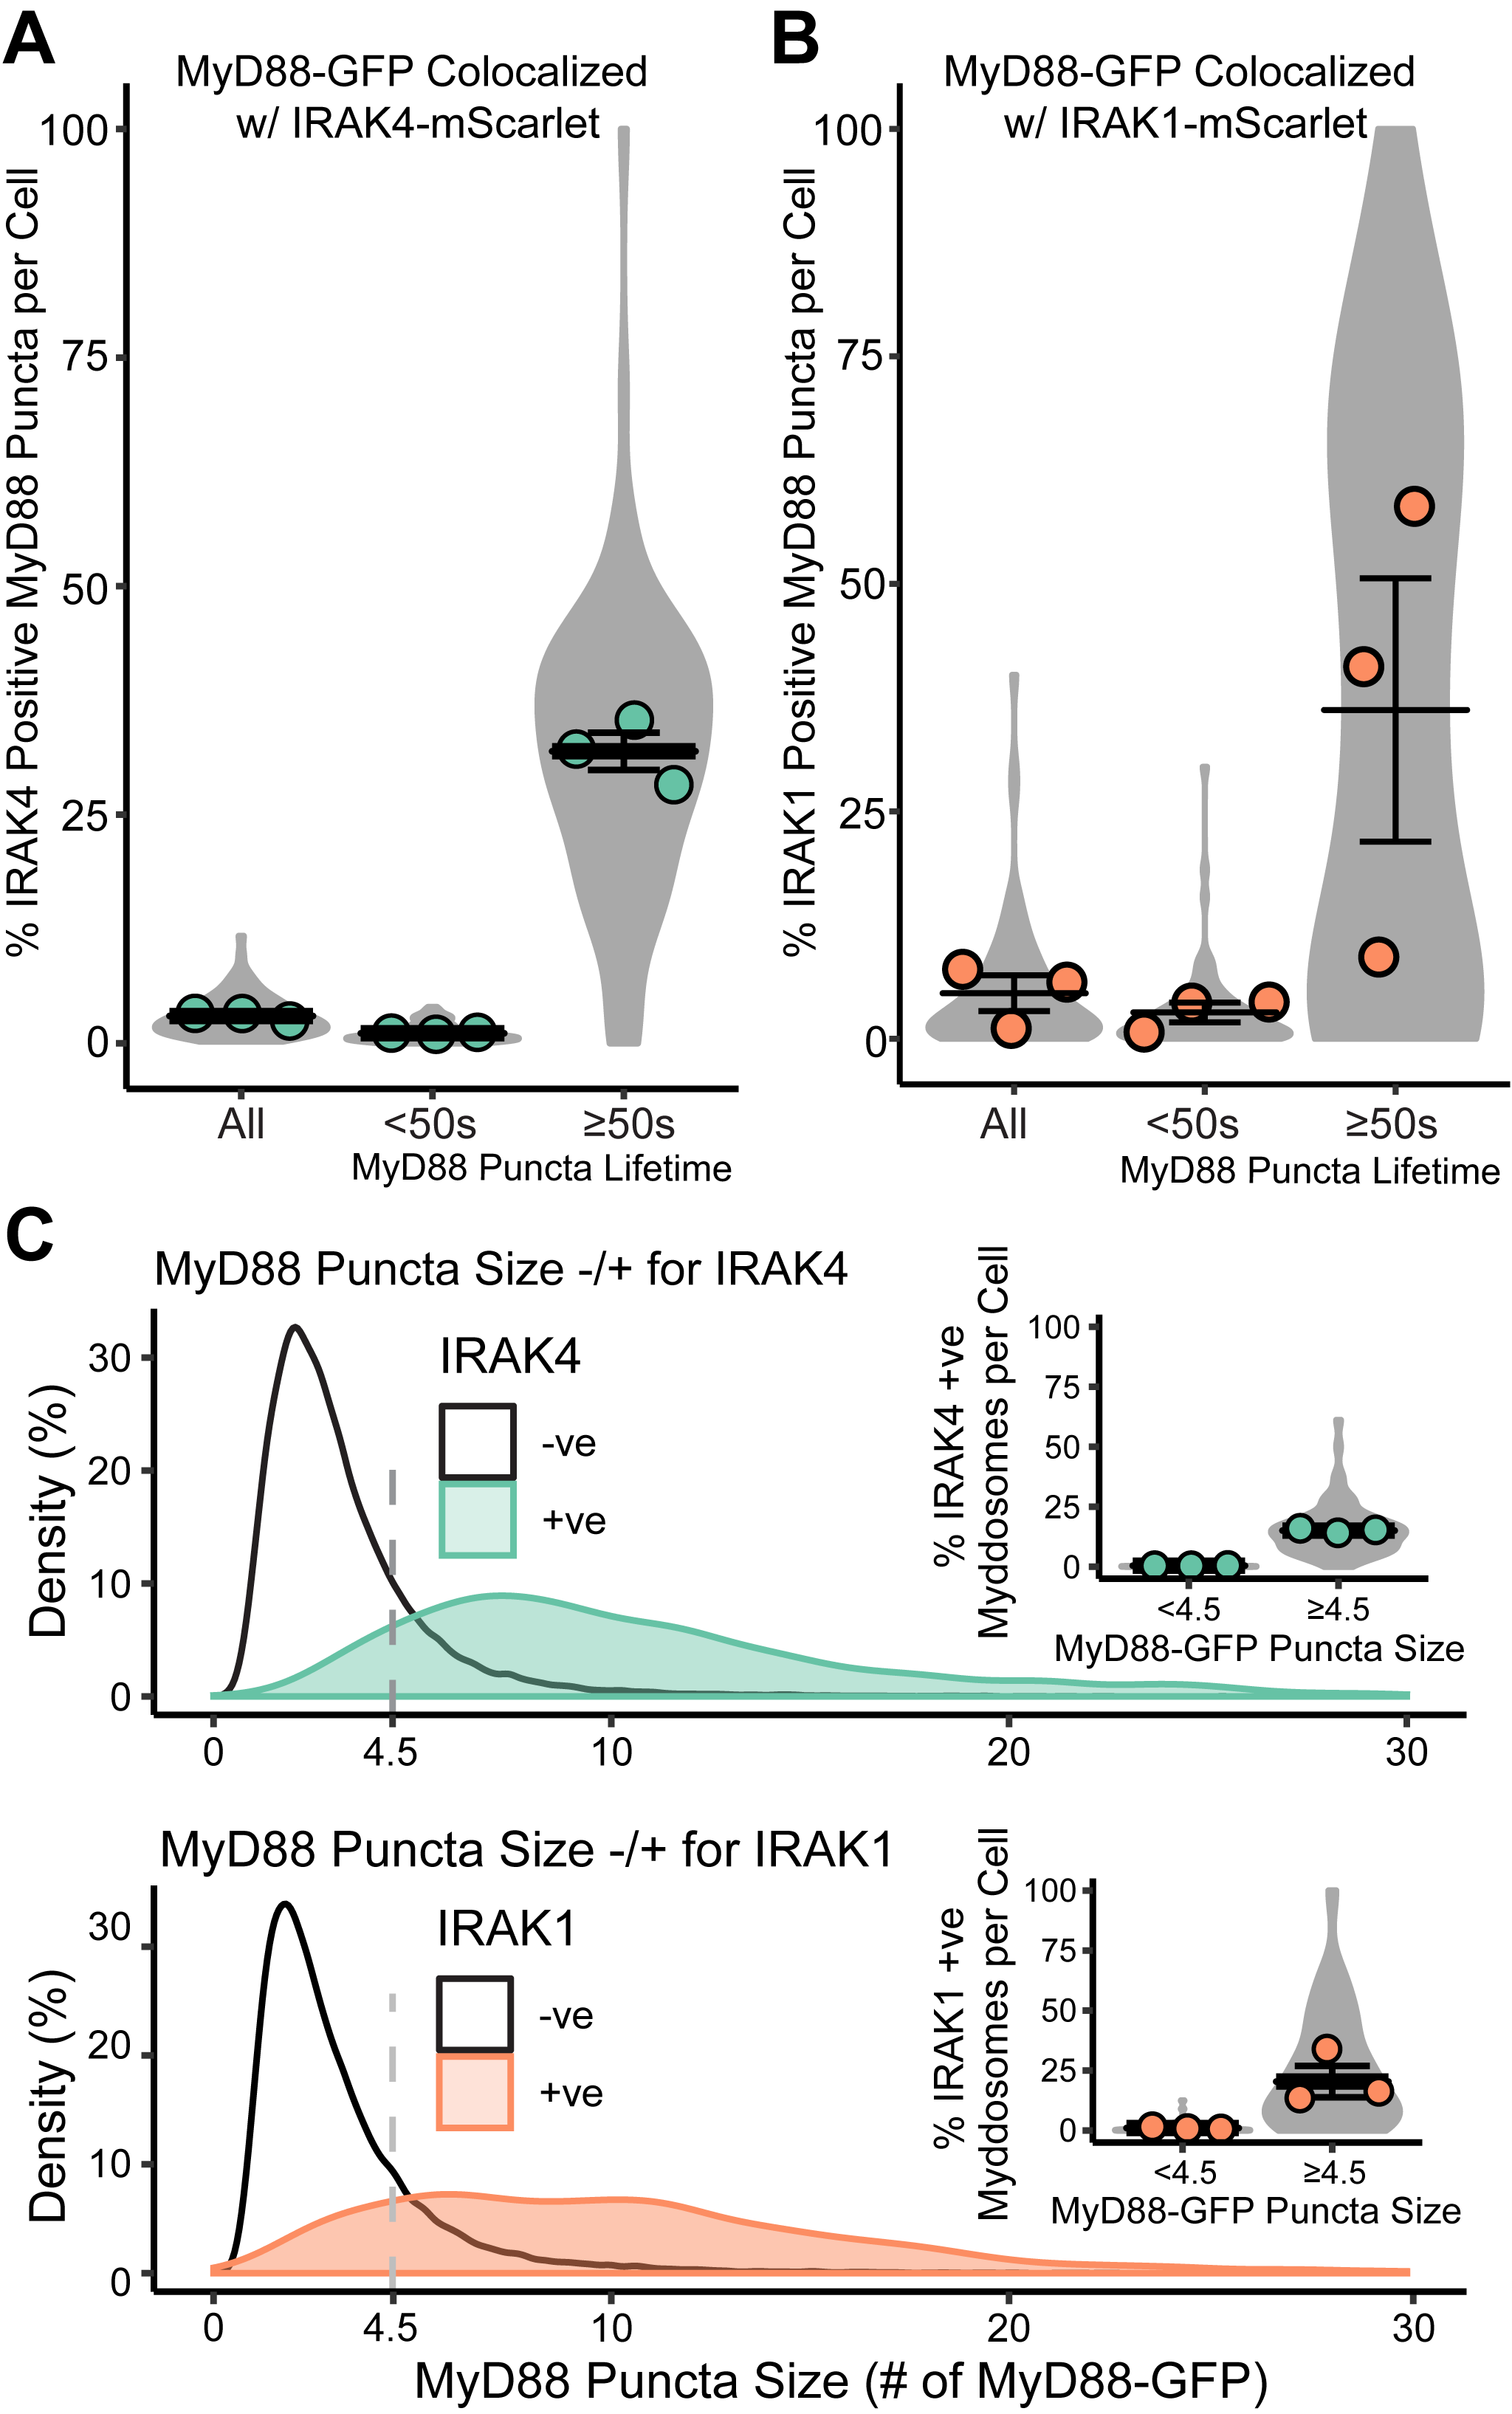
\includegraphics[width=\textwidth, height=\textheight, keepaspectratio]{jcb/fig4b.png}}
\captionsetup{parbox=none}
\captionof{figure}[IRAK4 and IRAK1 are recruited to larger MyD88 oligomers]{\textbf{IRAK4 and IRAK1 are recruited to larger MyD88 oligomers.}
\\
\\
(A-B) Quantification of the percentage of MyD88-GFP puncta per cell that colocalizes with IRAK4 (A) or IRAK1 (B) for all puncta and puncta with lifetimes under 50 seconds or at least 50 seconds. Violin plots (in gray) show the distribution of individual cell measurements. Colored dots superimposed on violin plots correspond to the average value in the independent experiments (n = 3 for IRAK4/1; each replicate encompasses measurements from 16--34 cells). Bars represent mean $\pm$ SEM.
\\
\\
(C) Density plot showing the distribution of MyD88 oligomer size (number of MyD88-GFP monomers is derived from the maximum intensity divided by the average intensity of GFP) for MyD88 puncta that are positive (+ve) or negative (-ve) for IRAK4 (top) or IRAK1 (bottom). Inset: Percentage of MyD88-GFP puncta per cell that colocalizes with IRAK4 or IRAK1 with a maximum intensity of under 4.5\times GFP or at least 4.5\times GFP. Violin plots show the distribution of individual cell measurements. Colored dots superimposed on the violin plots correspond to the mean value for the independent experiments (n = 3, IRAK4; n = 3, IRAK1). Bars represent mean $\pm$ SEM.
\\
\\
(Imaging data captured by Fakun Cao and the thesis author. Analysis, plots done by the thesis author. Figure, descriptions extracted from \autocite{Deliz-Aguirre_2021}.)}
\label{p1:4b}
\end{centering}

Lin et al. proposed that Myddosomes assemble sequentially based on their findings of the solved crystal structure \autocite{Lin_2010}. Yet, structural studies are spatiotemporally limited, and cannot easily resolve heterogeneity and intermediates. To investigate this model of sequential assembly, I identified when MyD88 and IRAK4 or IRAK1 appeared at a given location--a puncta. Then, I calculated the time delay between the MyD88 and IRAK4 or IRAK1 signal appearing. This is called the recruitment time, and it is illustrated in Fig.~\ref{p1:4c}A. I repeated this process for all MyD88 puncta that had IRAK4/1, and recorded it. Due to the noisy signal of small puncta, the output table was validated manually by Viviane Fenk and Marcus J. Taylor. I then plotted recruitment times as a histogram and as a density plot (Fig.~\ref{p1:4c}B). As we can see in the left-shifted green curve, almost all IRAK4 was recruited in under 25 seconds, the average being 14 seconds (Fig.~\ref{p1:4c}B). As we can see in the right-shifted wide orange curve, IRAK1 was still being recruited after 25 seconds, with the average at 41 seconds (Fig.~\ref{p1:4c}B).

The different timings establish that the Myddosome assembles sequentially (Fig.~\ref{p1:4c}C). Further corroborating the average recruitment time is its propagation of variance. Compared to IRAK4, IRAK1 had a wider distribution of recruitment times. This is to be expected in a sequentially assembling protein complex because, like a relay race, the delays in recruitment times accumulate (see Fig.~\ref{p2:D2} for an explanation).

Having established that the Myddosome assembles sequentially, I sought to answer what is the functional role of IRAK4 and IRAK1 in Myddosome complexes.


\begin{centering}
\centering{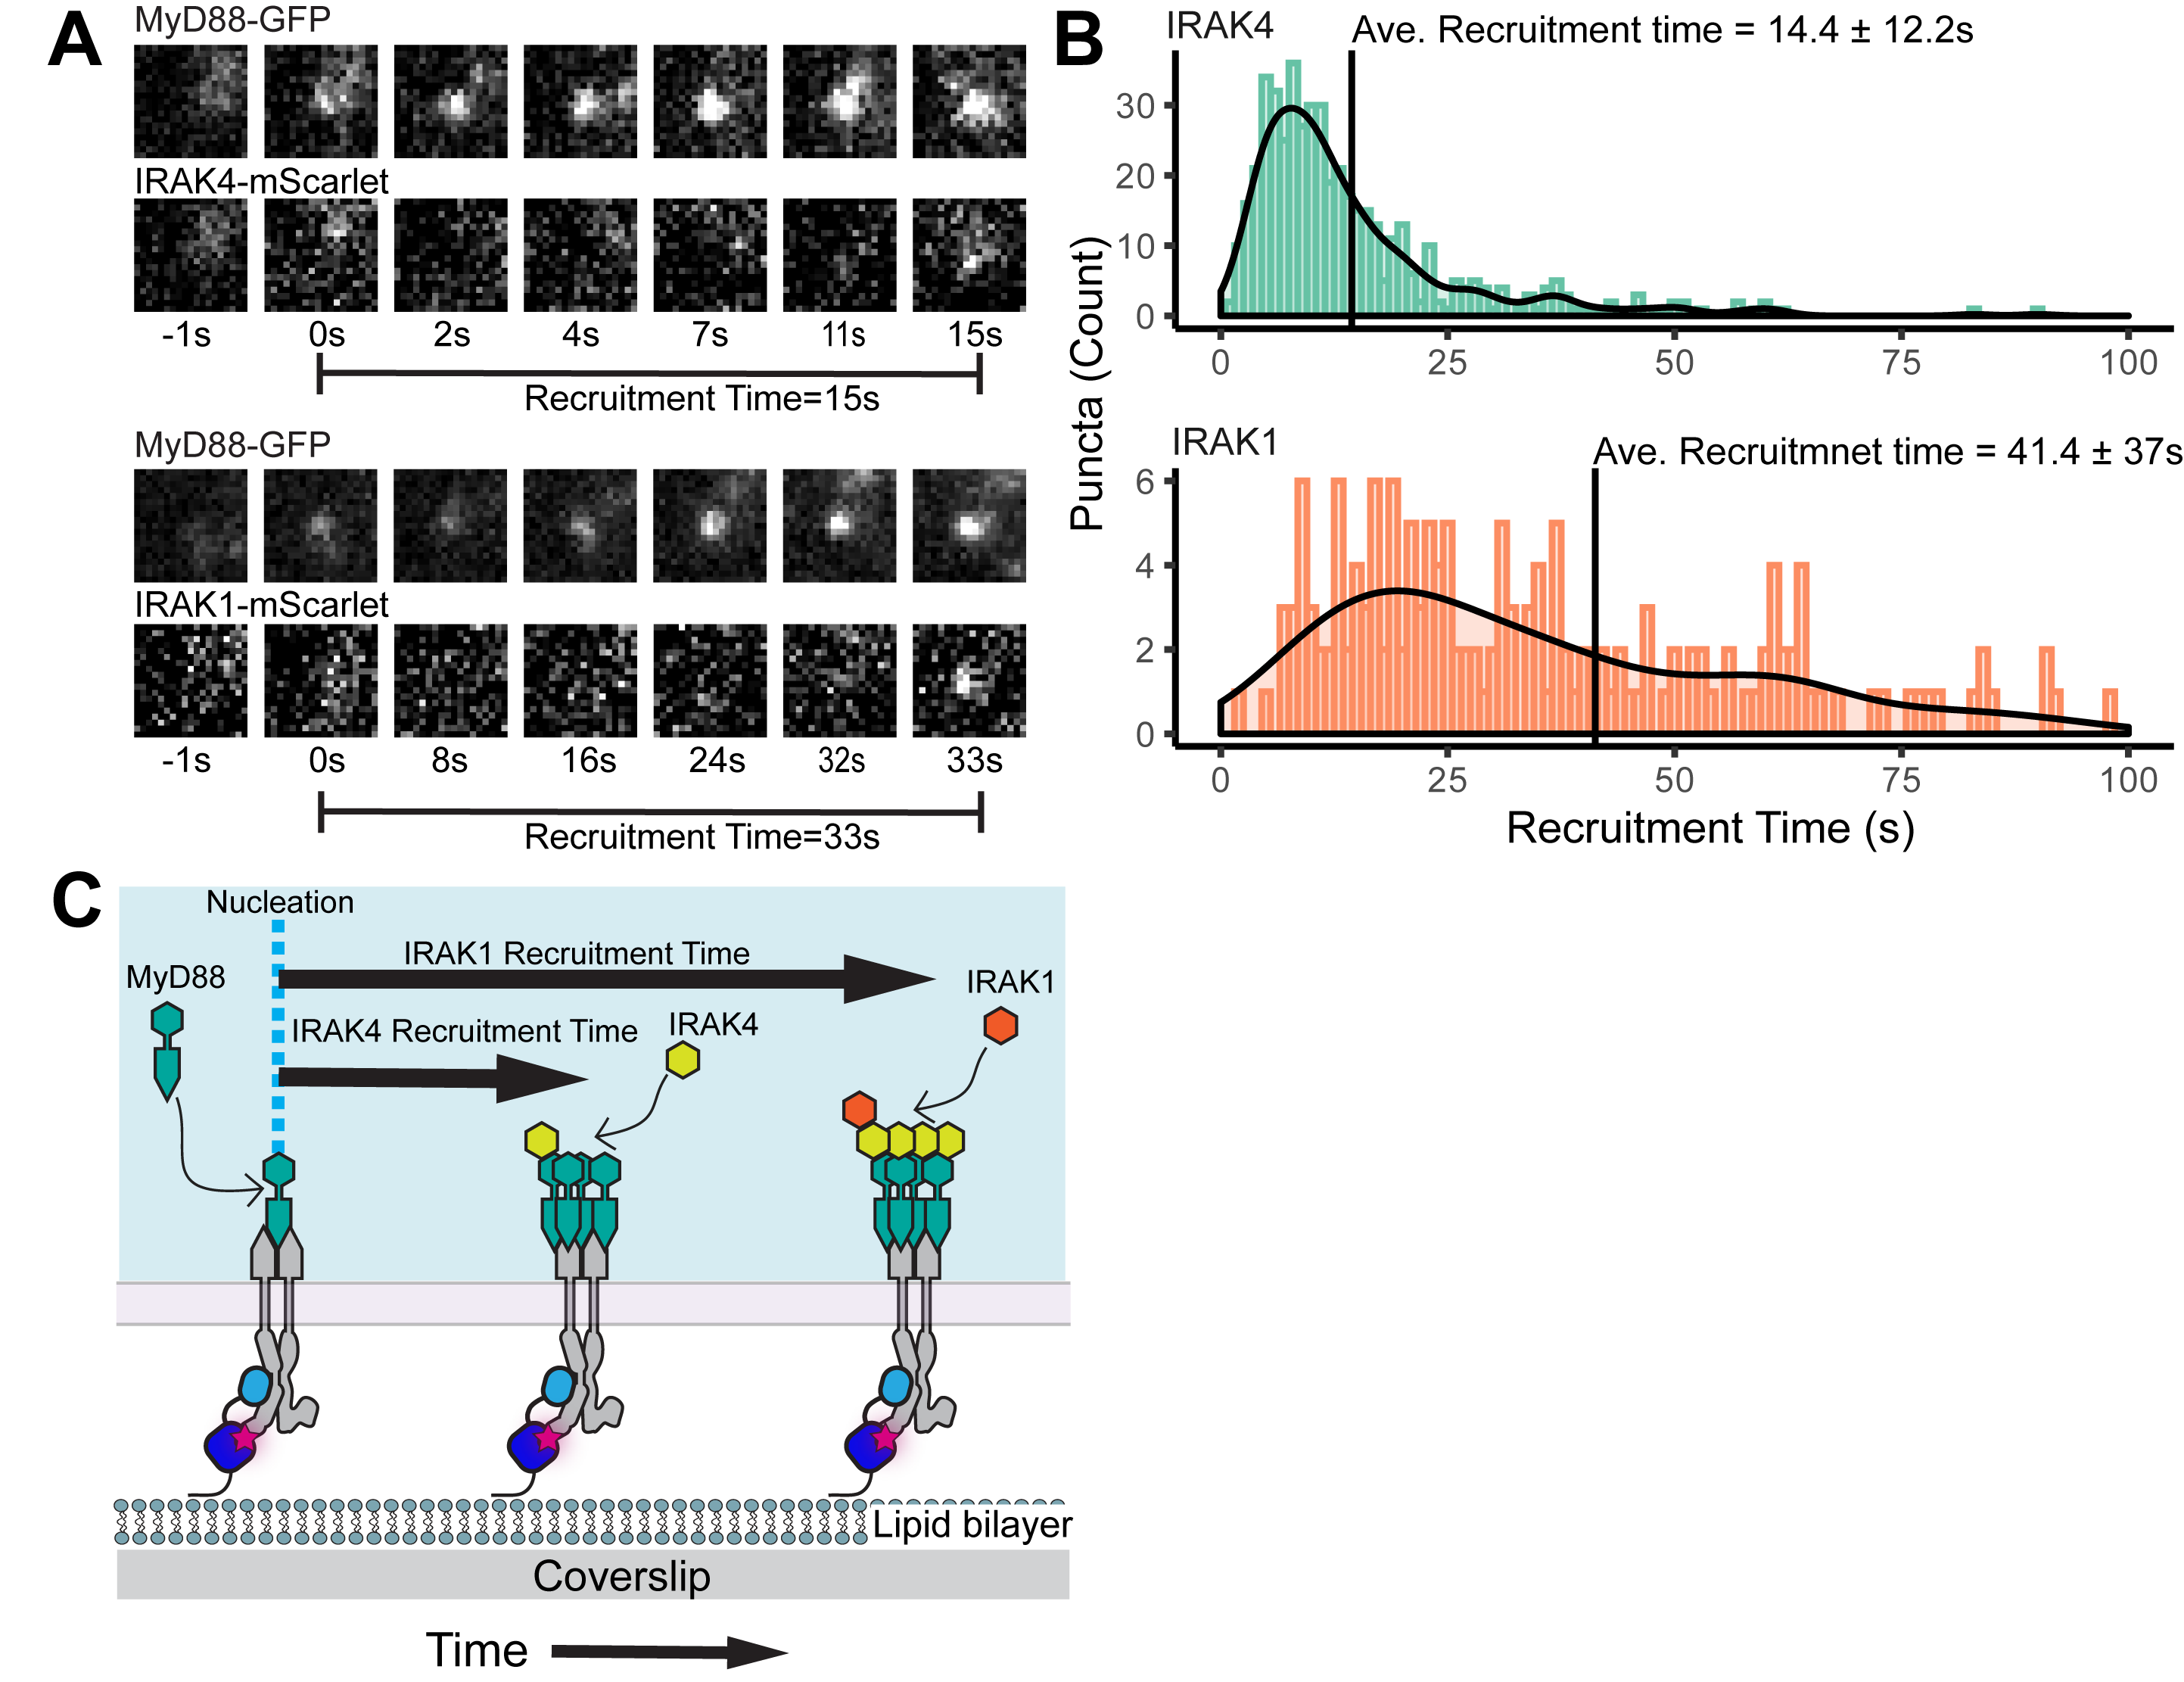
\includegraphics[width=\textwidth, height=\textheight, keepaspectratio]{jcb/fig4c.png}}
\captionsetup{parbox=none}
\captionof{figure}[IRAK4 and IRAK1 are recruited sequentially]{\textbf{IRAK4 and IRAK1 are recruited sequentially.} Analysis of IRAK4 and IRAK1 recruitment time during Myddosome assembly. Recruitment time was defined as the time interval from Myddosome nucleation (e.g., time = 0 seconds when MyD88-GFP puncta appears) to the appearance of IRAK4/1-mScarlet. Middle: 
\\
\\
(B) Time series of TIRF images showing MyD88-GFP nucleation followed by IRAK4-mScarlet (top time series) or IRAK1-mScarlet (bottom time series) recruitment. Histogram of IRAK4 (n = 482 recruitment events, combined from 30 cells) and IRAK1 (n = 170 recruitment events, combined from 40 cells) recruitment times overlaid with the density plot of the distribution. Black horizontal lines on the histograms denote the average recruitment time (mean $\pm$ SD). Ave., average.
\\
\\
(C) MyD88 assembles first, then IRAK4, and lastly, IRAK1.
\\
\\
(A: Panel courtesy of Marcus Taylor with images acquired by Fakun Cao and the thesis author. B:  Imaging data courtesy of Fakun Cao, and analysis, plots done by the thesis author, and curated by Marcus Taylor and Viviene Fink. C: Panel courtesy of Marcus J. Taylor. Figure, descriptions extracted from \autocite{Deliz-Aguirre_2021}.)}
\label{p1:4c}
\end{centering}

\section{IRAK4 regulates MyD88 oligomer size}
\sectionmark{IRAK4 regulates MyD88}
Previous mouse KO models have demonstrated that IRAK4/1 are essential for IL-1R/TLR signal transduction \autocite{Thomas_2003}\autocite{Wang_2009}\autocite{Jain_2020}. Yet, their functional role remains unclear. To interrogate the function of IRAK4 and IRAK1, I sought to establish what effect knocking-out IRAK4 or IRAK1 would have on MyD88. I had three hypotheses. (1) Because IRAK4 inhibited Myddosomes are more stable (De Nardo et al., 2018), my first hypothesis was that IRAK4/1 caps oligomerization, and their knockout would result in large long-lived MyD88 puncta. (2) My second hypothesis was that IRAK4/1 are there for stability, and their knockout would result in small short-lived unstable MyD88 puncta. (3) Lastly, my third hypothesis was that IRAK4\textsuperscript{KO} and IRAK1\textsuperscript{KO} would have no effect on the lifetime and size of MyD88. Elke Ziska and Nichanok Auevechanichkul used CRISPR/Cas9 to generate a MyD88-eGFP IRAK4\textsuperscript{KO} and MyD88-eGFP IRAK1\textsuperscript{KO} cell lines. 

Consistent with the literature \autocite{DeFelice_2019}\autocite{Suzuki_2002}, these knock-out cell lines did not signal (Fig.~ref{p1:S2}A). As we can see in Fig.~\ref{p1:6a}A-B, wild-type (WT) MyD88 and IRAK1\textsuperscript{KO} appear to have comparable brightness. This suggests that for IRAK1, the no change in MyD88 after IRAK1\textsuperscript{KO} (third) hypothesis is correct. However, as we can appreciate in Fig.~\ref{p1:6a}C, IRAK4\textsuperscript{KO} cells have unusually bright, long-lived MyD88 puncta. This suggests that for IRAK4, the bright long lived MyD88 after IRAK4\textsuperscript{KO} (first) hypothesis is correct.

In the absence of IRAK4/1, MyD88 was recruited to the IL-1R after IL-1 stimulation in IRAK4/1\textsuperscript{KO} cell lines. The findings preliminarily indicate that while IRAK1\textsuperscript{KO} does not seem to affect the dynamics of MyD88, IRAK4\textsuperscript{KO} enhances the brightness and longevity of MyD88 assemblies. To further corroborate these initial observations, I quantified the images and performed statistical analysis to determine if MyD88 differences in IRAK4\textsuperscript{KO} and IRAK1\textsuperscript{KO} are statistically significant.


\begin{centering}
\centering{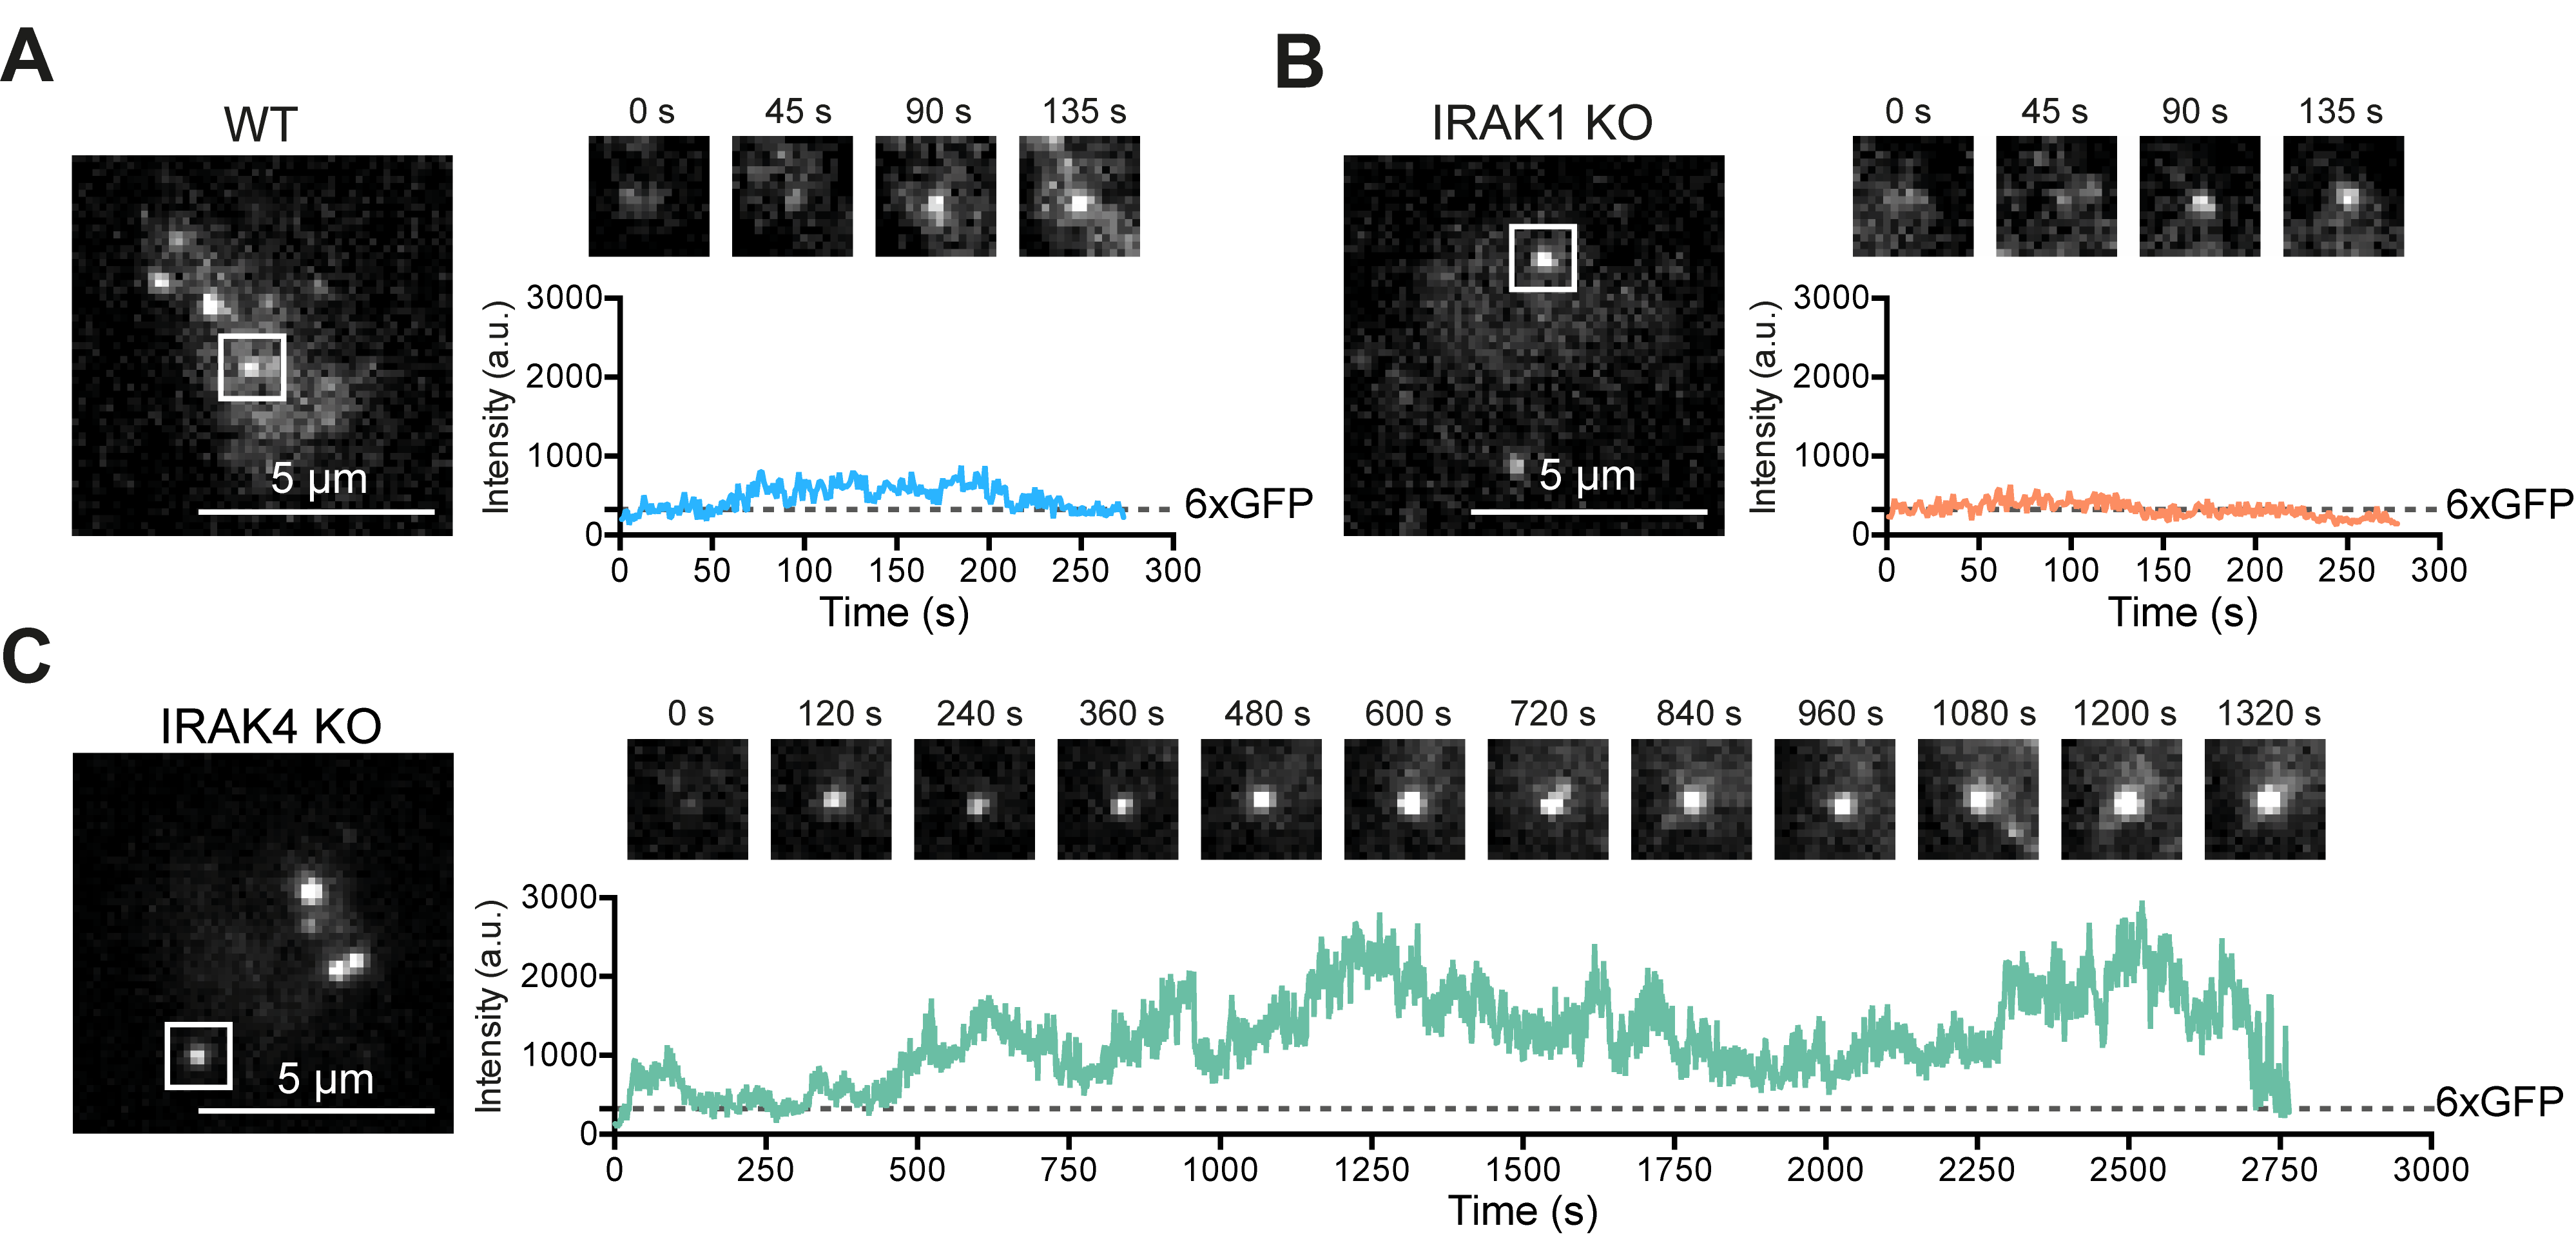
\includegraphics[height=\textwidth, width=\textheight, angle=-90, keepaspectratio]{jcb/fig6a.png}}
\captionsetup{parbox=none}
\captionof{figure}[IRAK4 KO leads to large MyD88 oligomers]{\textbf{IRAK4 KO leads to super MyD88 oligomers.} TIRF images of MyD88-GFP in EL4 WT, (A) IRAK1 KO (B), and IRAK4 KO (C) cells. Time-series TIRF images from the region of interest (white box) showing MyD88 puncta. A fluorescence intensity time trace from each time series is shown below.
\\
\\
(Images and intensity plots courtesy of Fakun Cao. D-F: Images acquired by Fakun Cao and analyzed, plotted by the thesis author. Figure, descriptions extracted from \autocite{Deliz-Aguirre_2021}.)}
\label{p1:6a}
\end{centering}

I hypothesized that if MyD88 dynamics are unchanged (Fig.~\ref{p1:3c}B), then most puncta will be small and dim (Fig.~\ref{p1:3b}D). To be able to detect the change in MyD88 size and lifetime, I would need to bin the lifetime as before to identify large MyD88 (Fig.~\ref{p1:3b}). My alternate hypothesis was that if the dynamics changed, then binning lifetime would enable me to detect a change in the molecular dynamics. Binning by lifetime would therefore offer a twofold benefit.

After analyzing the IRAK4/1\textsuperscript{KO} images, I plotted the MyD88 size (y-axis) by cell line (x-axis). I then binned the data based on lifetime (sub-plots). As we can see on the left side of Fig.~\ref{p1:6b}A (Lifetime <50s), short-lived MyD88 puncta in wild-type (WT, negative control) and IRAK4/1 knockout cell lines have comparable brightness because the violin plots (cell replicate means) and dots (image replicate means) have comparable height on the y-axis (MyD88 size).\footnote{Intensity binned in Fig.~\ref{p1:S5}A-B} To confirm intuition, I performed a two-tailed unpaired Student's t-test on the image replicates (dots). IRAK4/1 knockout produced no statistically significant difference in the MyD88 size of short-lived MyD88 puncta to WT (p = 0.31 and p = 0.68, respectively). Therefore, knocking-out IRAK4/1 does not significantly affect the MyD88 dynamics and size in short-lived puncta. However, as we can see on the right side of Fig.~\ref{p1:6b}A, when we focus on the long-lived MyD88 puncta (Lifetime $\geq$50s), we can see that IRAK4\textsuperscript{KO} cell lines produce unusually bright MyD88 puncta because we observe events brighter than 20\times MyD88 in the replicate means (violin plot).\footnote{Intensity binned in Fig.~\ref{p1:S5}B} To confirm, I performed the same statistical analysis as with the short-lived. Compared to WT, IRAK4\textsuperscript{KO} had statistically-significant larger sizes (p = 0.015), but not IRAK1\textsuperscript{KO} (p = 0.17). As a positive control, we reconstituted IRAK4 in the IRAK4\textsuperscript{KO} cell line. It showed no statistically-significant difference to WT in short-lived MyD88 (p = 0.17) nor long-lived MyD88 (p = 0.68). This confirms that IRAK4\textsuperscript{KO} produces unusually large MyD88 puncta. However, it does not establish if these long-lived bright MyD88 also have unusually long lifetimes.

The puncta images hint that IRAK4\textsuperscript{KO} (Fig.~\ref{p1:6a}) lived longer. To confirm, I plotted a histogram of the lifetime of MyD88 puncta (x-axis) with the frequency in $\log(x+1)$ scale (y-axis), binned by size (4.5\times MyD88), similar to Fig.~\ref{p1:3b}. Dim puncta (<4.5\times MyD88 in red) have similar histograms, none surpassing 1000 seconds (Fig.~\ref{p1:6b}B). However, when only long-lived (at least 4.5\times MyD88 in blue) are examined, it is clear only IRAK4\textsuperscript{KO} have puncta living longer than 1500 seconds (Fig.~\ref{p1:6b}B).

To understand if there were any changes in MyD88 kinetics (growth dynamics), I compared the lifetime (x-axis) against the change in intensity (y-axis), just like it was done in Fig.~\ref{p1:3c}B. Notice how in Fig.~\ref{p1:6b}C, growth and lifetime are correlated, including on IRAK4\textsuperscript{KO}. Also notice how the slopes of the regression line are comparable. These indicate that the kinetics have not changed. To confirm, Fakun Cao performed FRAP analysis and showed that MyD88 recovers after photobleaching only in IRAK4\textsuperscript{KO} (see Fig. 7A of \autocite{Deliz-Aguirre_2021}.

The data shows that when IRAK4 is present (WT), MyD88 size reaches a size limit which suggests it is being regulated (Fig.~\ref{p1:6b}A). In the absence of IRAK4, cells produce unusually long MyD88 oligomers (Fig.~\ref{p1:6b}A) that are long-lived (Fig.~\ref{p1:6b}B) and grow at a similar rate to WT MyD88 (Fig.~\ref{p1:6b}C). Therefore, this data has shown that IRAK4 regulates MyD88 oligomer size. 


\begin{centering}
\centering{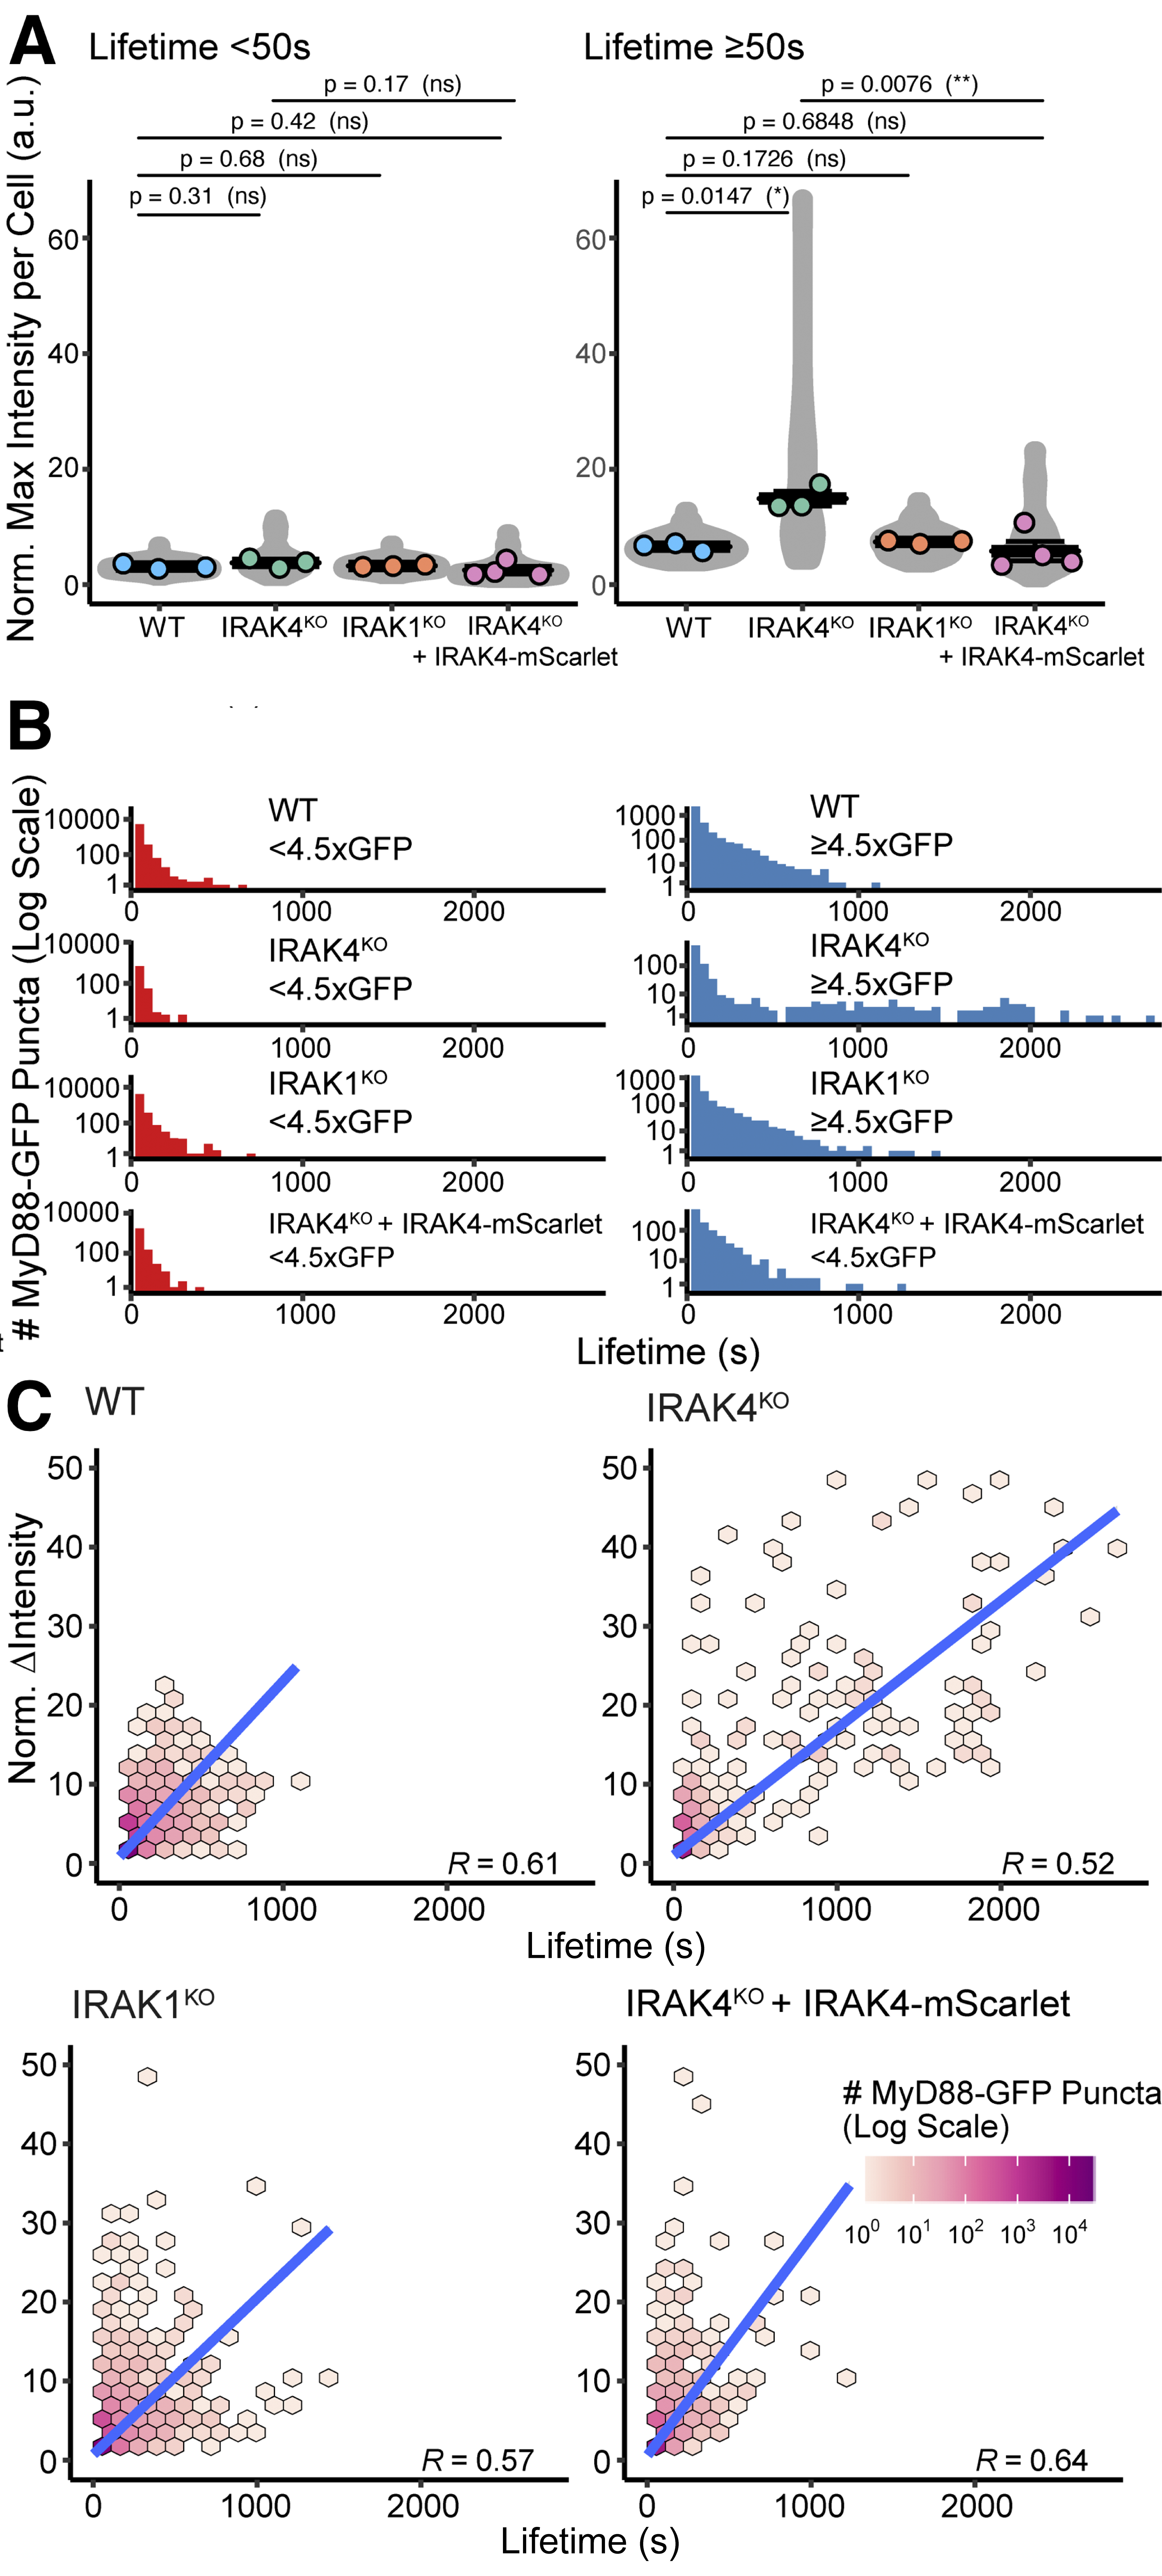
\includegraphics[width=\textwidth, height=\textheight, keepaspectratio]{jcb/fig6b.png}}
\captionsetup{parbox=none}
\captionof{figure}[IRAK4 regulates MyD88 oligomerization]{\textbf{IRAK4 regulates MyD88 oligomerization.}
\\
\\
(A) Quantification of the maximum intensity of MyD88-GFP puncta per cell with lifetimes of under 50 seconds or at least 50 seconds. Violin plots show the distribution of individual cell measurements. Colored dots superimposed on violin plots correspond to the average value in the independent experiments (n = 3 or 4 experimental replicates; encompasses measurements from 10 to 47 cells). Bars represent mean $\pm$ SEM. P values were calculated using a two-tailed unpaired Student's t test.
\\
\\
(B) Distribution of lifetimes for tracked MyD88-GFP puncta with a maximum intensity of under 4.5\times or at least 4.5\times GFP in WT (n = 73,180 for under 4.5\times GFP and n = 24,631 for at least 4.5\times GFP), IRAK4 KO (n = 18,478 for under 4.5\times GFP and n = 9,795 for at least 4.5\times GFP), and IRAK1 KO (n = 63,382 for under 4.5\times GFP and n = 19,735 for at least 4.5\times GFP) and IRAK4 KO + IRAK4-mScarlet (n = 18,764 for under 4.5\times GFP and n = 5,627 for at least 4.5\times GFP) cells. MyD88-GFP puncta lifetimes collated from 3 or 4 experimental replicates.
\\
\\
(C) 2D histogram of MyD88-GFP puncta lifetime versus fluorescent intensity change for WT (n = 64,149), IRAK4 KO (n = 13,960), IRAK1 KO (n = 54,551), and IRAK4 KO + IRAK4-mScarlet (n = 18,154) cells. Linear fit is shown as a blue line. The coefficient used is Spearman’s rank correlation coefficient. Max, maximum; Norm., normalized.
\\
\\
(Images acquired by Fakun Cao and analyzed, plotted by the thesis author. Figure, descriptions adapted from \autocite{Deliz-Aguirre_2021}.)}
\label{p1:6b}
\end{centering}

In closing, my analysis showed dynamic equilibrium with small transient MyD88 assemblies being unstable, with only a few becoming bright and long-lived (Fig.~\ref{p1:3b}). Only this population is able to recruit downstream proteins IRAK4/1 which could potentially lead to cellular activation (Fig.~\ref{p1:3d}). I identified that the Myddosome assembles \emph{de novo} with on-demand (inducible) oligomerization and sequential steps (Fig.~\ref{p1:4b}-~\ref{p1:4c}). The observed formation of aberrantly large MyD88 assemblies in IRAK4\textsuperscript{KO} cells underpins the role of IRAK4 as a negative regulator of MyD88 oligomerization (Fig.~\ref{p1:6b}).


\begin{centering}
\centering{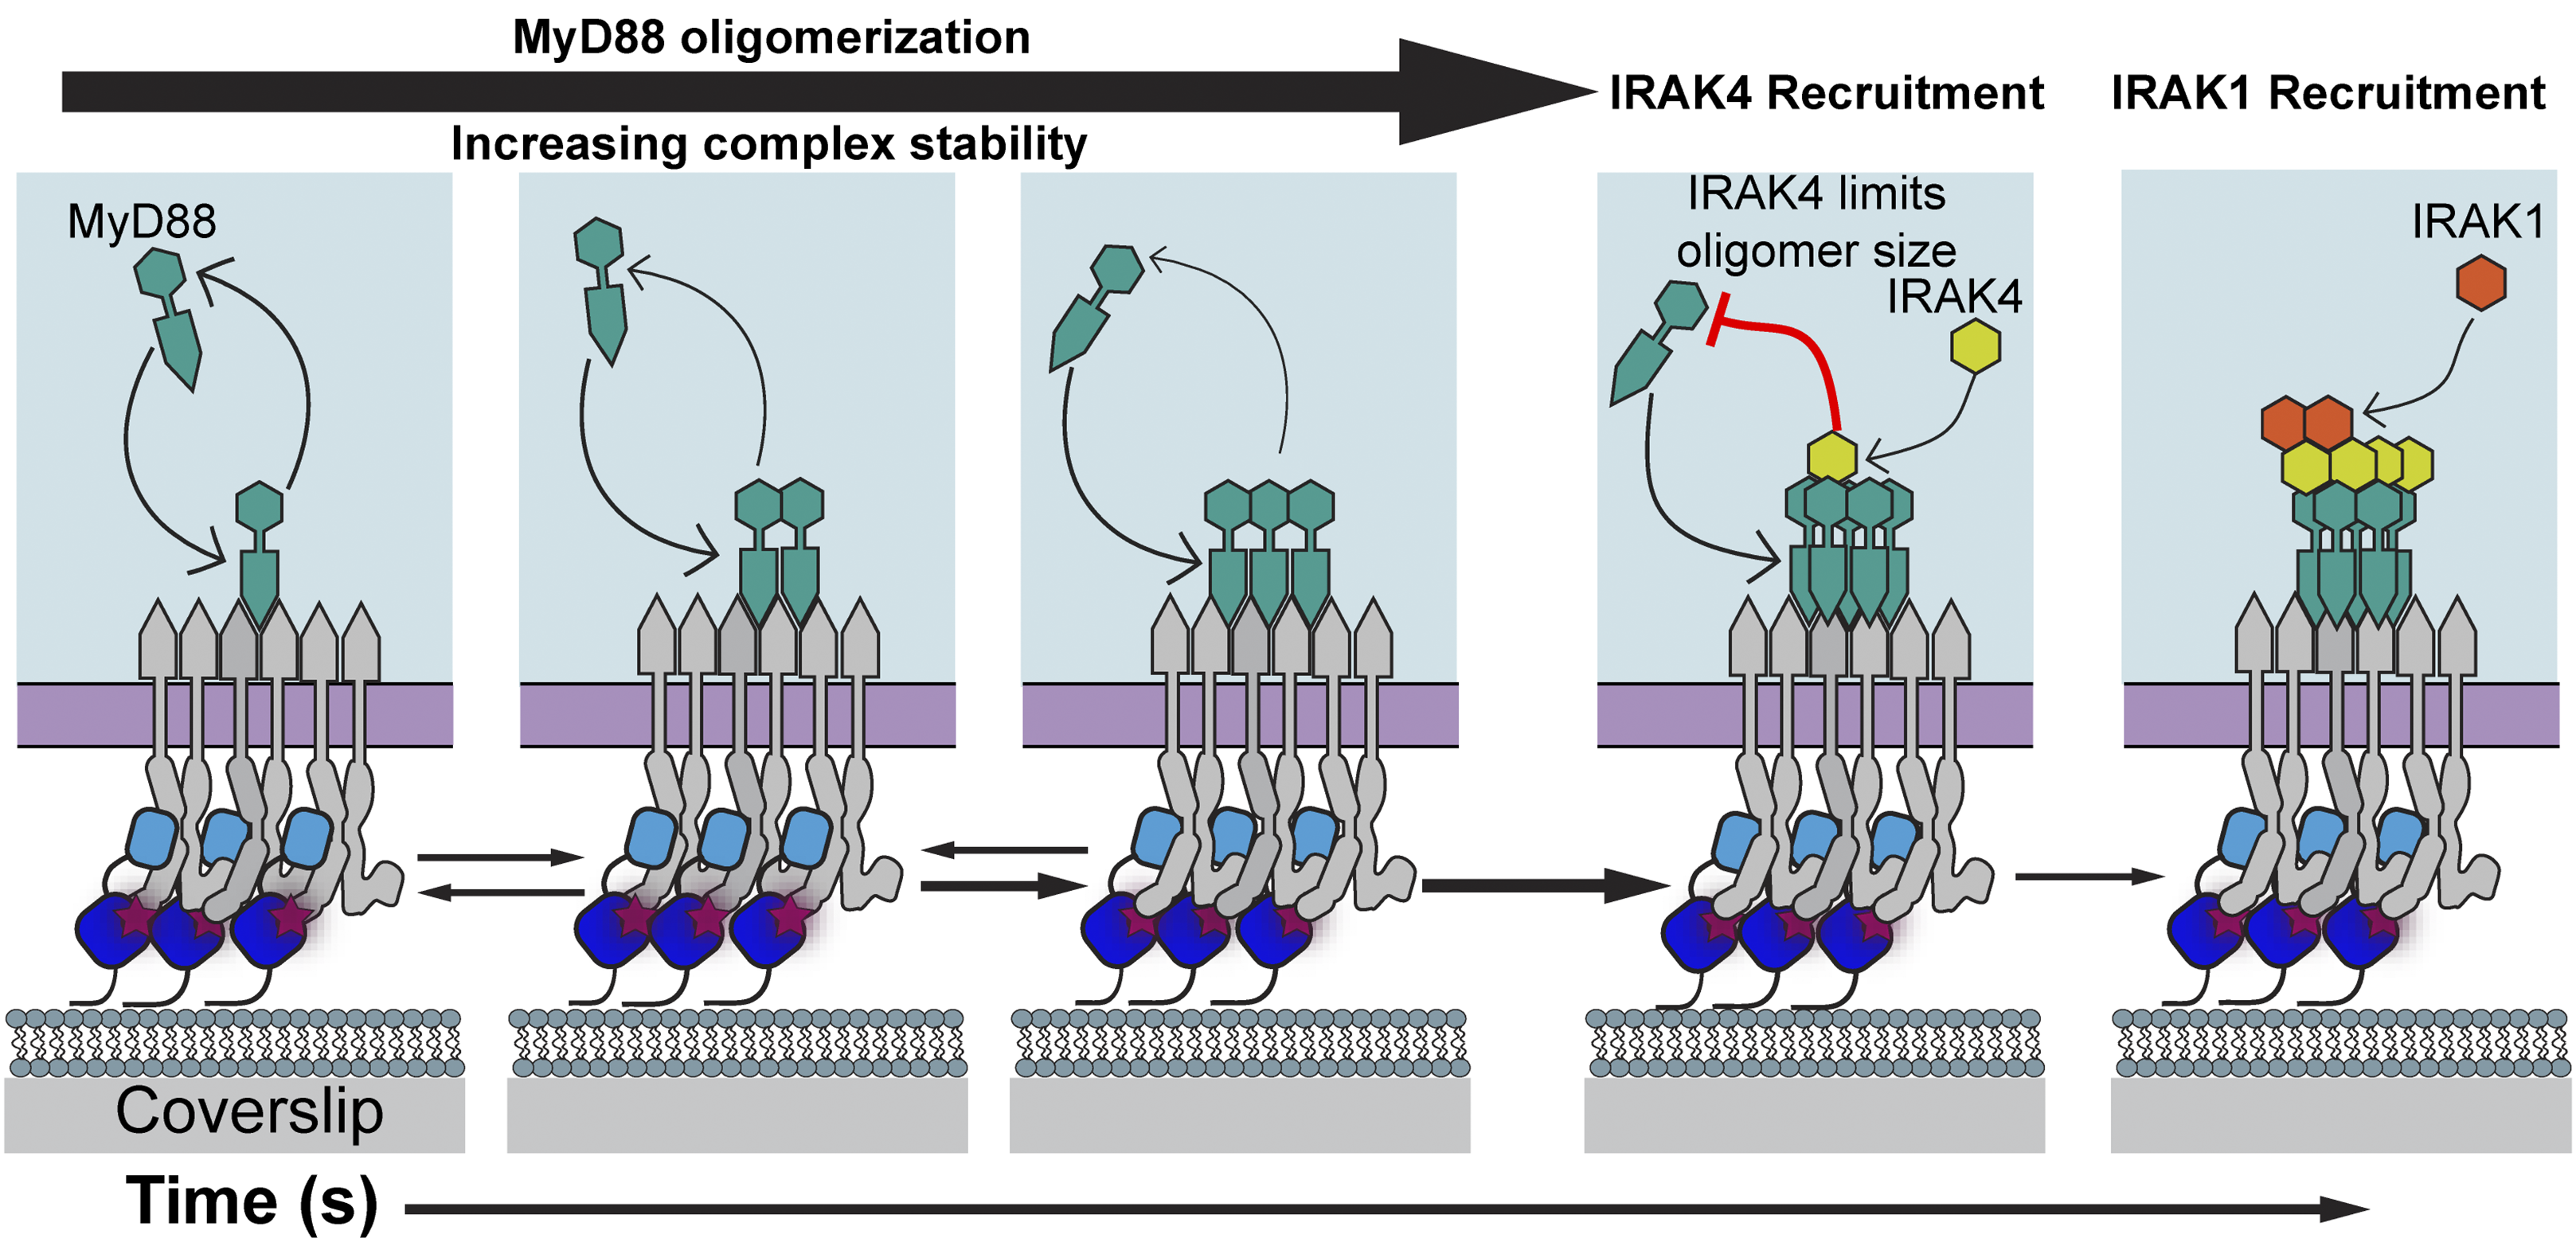
\includegraphics[width=\textwidth, height=\textheight, keepaspectratio]{jcb/fig7.png}}
\captionsetup{parbox=none}
\captionof{figure}[Myddosomes oligomerization is ligand-induced and sequential with IRAK4 regulating MyD88 oligomer size]{\textbf{Myddosomes oligomerization is ligand-induced and sequential with IRAK4 regulating MyD88 oligomer size.} Speculative model describing Myddosome assembly. MyD88 recruitment to the IL1-bound IL1R nucleates MyD88 oligomerization. Initially, the small oligomer of MyD88 is unstable and can disassemble. However, as MyD88 oligomer size increases, so does complex stability, and the formation of larger MyD88 complexes triggers downstream signaling in the form of the sequential recruitment of IRAK4 followed by IRAK1.
\\
\\
(Diagram courtesy of Marcus Taylor. Figure, descriptions extracted from \autocite{Deliz-Aguirre_2021}.)}
\label{p1:f7}
\end{centering}

\chapter{The IL-1 pathway circuitry has coupled signalosome-modules with feedback loops}
\chaptermark{IL-1 pathway circuitry}
\label{chapter:p2}
\section{Motivation}
Once IL-1 comes in contact with the IL-1 receptor (IL-1R), a signaling cascade is triggered. The components of this signaling cascade are the Myddosome, TRAF6, the TAK1/TABs complex, the linear ubiquitin chain assembly complex complex, the IKK complex, and the NF-κB complex (see Introduction~\ref{chapter:pathway}, Fig.~\ref{img:pathway}). How protein monomers come together, that is the intermediary steps needed, to form the aforementioned protein complexes before NF-κB activation is poorly understood. As we show via direct imaging through TIRF microscopy (and presented at Results~\ref{chapter:p1}), the IL-1 signaling cascade events occur though the assembly of MyD88 punctate transient structures. How the signaling cascade is encoded in the physical interactions of pathways components within the structured cytoplasm of live cells has previously not been easy to study. This is partially due to the challenges inherent in imaging the single-molecule dynamics in live cells \autocite{Liu_2015}. Thus, the assembly choreography has not been fully described. There are indications that larger assemblies enhance signaling \autocite{Latty_2018}\autocite{Deliz-Aguirre_2021}\autocite{Cao_2023}. But outside the Myddosome \autocite{Deliz-Aguirre_2021}, the colocalization between MyD88 and downstream proteins have not been determined. Endpoint assays cannot reveal the regulatory mechanisms that exist within the IL-1 pathway.

In this chapter, I will unveil the modularity of the IL-1 signaling pathway. To accomplish this, I will first describe the assembly sequence of IL-1 pathway proteins. I will then describe the dependence of IL-1 pathway proteins assembly on instantaneous protein composition (described in the Introduction~\ref{section:pp}), asking what are the protein requirements for colocalization using two-color imaging of gene edited cell lines. Finally, I will use dynamical systems theory based visualizations tools (see also Introduction~\ref{section:pp}) to characterize the interactions of the protein components with each other. Together, I will present three distinct assays that all consistently detail the modular nature of the IL-1 pathway and its internal regulation.

\section{IL-1 pathway proteins condense and colocalize}
\sectionmark{Proteins colocalize}
There has been extensive biochemical characterization of the IL-1 pathway; however, methods like the often-employed pulldown assays have spatiotemporal limitations, have false positives, false negatives, may miss transient structures, and lack context \autocite{Ghavidel_2005}\autocite{Perry_2019}\autocite{Tabar_2022}. This study combines the advances in CRISPR/Cas9-based generation of fluorescently labeled cell lines, TIRF imaging and dynamic systems theory to overcome many of these limitations.

A comprehensive survey of IL-1 pathway protein dynamics has not been undertaken before. To investigate if the assembly and disassembly of IL-1 pathway proteins is modular, a comprehensive survey of the pathway was conducted using two-color imaging (Fig.~\ref{img:pathway}). Key proteins from various complexes were included: MyD88, IRAK4, and IRAK1 from the Myddosome; TRAF6 and TAB2 from the TAK1-TAB complex; HOIL1 from LUBAC; NEMO from the canonical IKK complex; NF-κB transcription factor subunit RelA (p65); and the deubiquitinase A20.

What is the assembly and disassembly mechanism of IL-1 pathway proteins? To address this, the previously described assay (Chapter~\ref{chapter:p1}) was employed (Fig.~\ref{p2:system}A). The assay facilitates the validation of pulldown and structural experiments, shedding light on the interplay of specific proteins in the IL-1 pathway. The results of this assay have been described in Chapter~\ref{chapter:p1} and allowed us to show that MyD88 oligomer size works as a physical threshold to trigger IL-1 induced Myddosome signaling.

Using light microscopy (Fig.~\ref{p2:system}A), all tagged proteins, as downstream as RelA of the NF-κB complex, exhibited observable and persistent colocalization with MyD88 at the cell surface (Fig.~\ref{p2:system}B), thus I have discovered that all key IL-1 pathway pathway proteins colocalize with MyD88, assembling into puncta (condensates) with an ordered sequence \autocite{Lin_2010}\autocite{Ye_2002}\autocite{Kelsall_2019}\autocite{Tarantino_2014}\\\autocite{Jäättelä_1996}\autocite{Sizemore_1999}\autocite{Takaesu_2000}\autocite{Cohen_2020}. The ability to image the heterogenous assembly dynamics of the survey IL-1 pathway component proteins, provides a powerful new probe for studying the regulated chemical dynamics of the IL-1 pathway. The never before seen association dynamics led me to the discovery of modules within the IL-1 pathway (see Results~\ref{chapter:p2}).

In this chapter, I describe how the chemical dynamics of the IL-1 pathway reveal a modular architecture. I will do this in three steps: (1) I will first provide evidence for the existence of two modules from following the association kinetics of IL-1 pathway components (Results~\ref{section:IL1_seq}). (2) I will next use FRAP (Fluorescence Recovery After Photobleaching) as an independent way to corroborate the existence of modules and to show that the modules exhibit distinct chemical dynamics.(Results~\ref{section:biophysical}). (3) Finally, I will describe a novel analysis framework, phase portrait analysis, and will use this to provide a third independent method for modularity and also to probe the feedback between modules (Results~\ref{section:two_dynamics}).


\begin{centering}
\centering{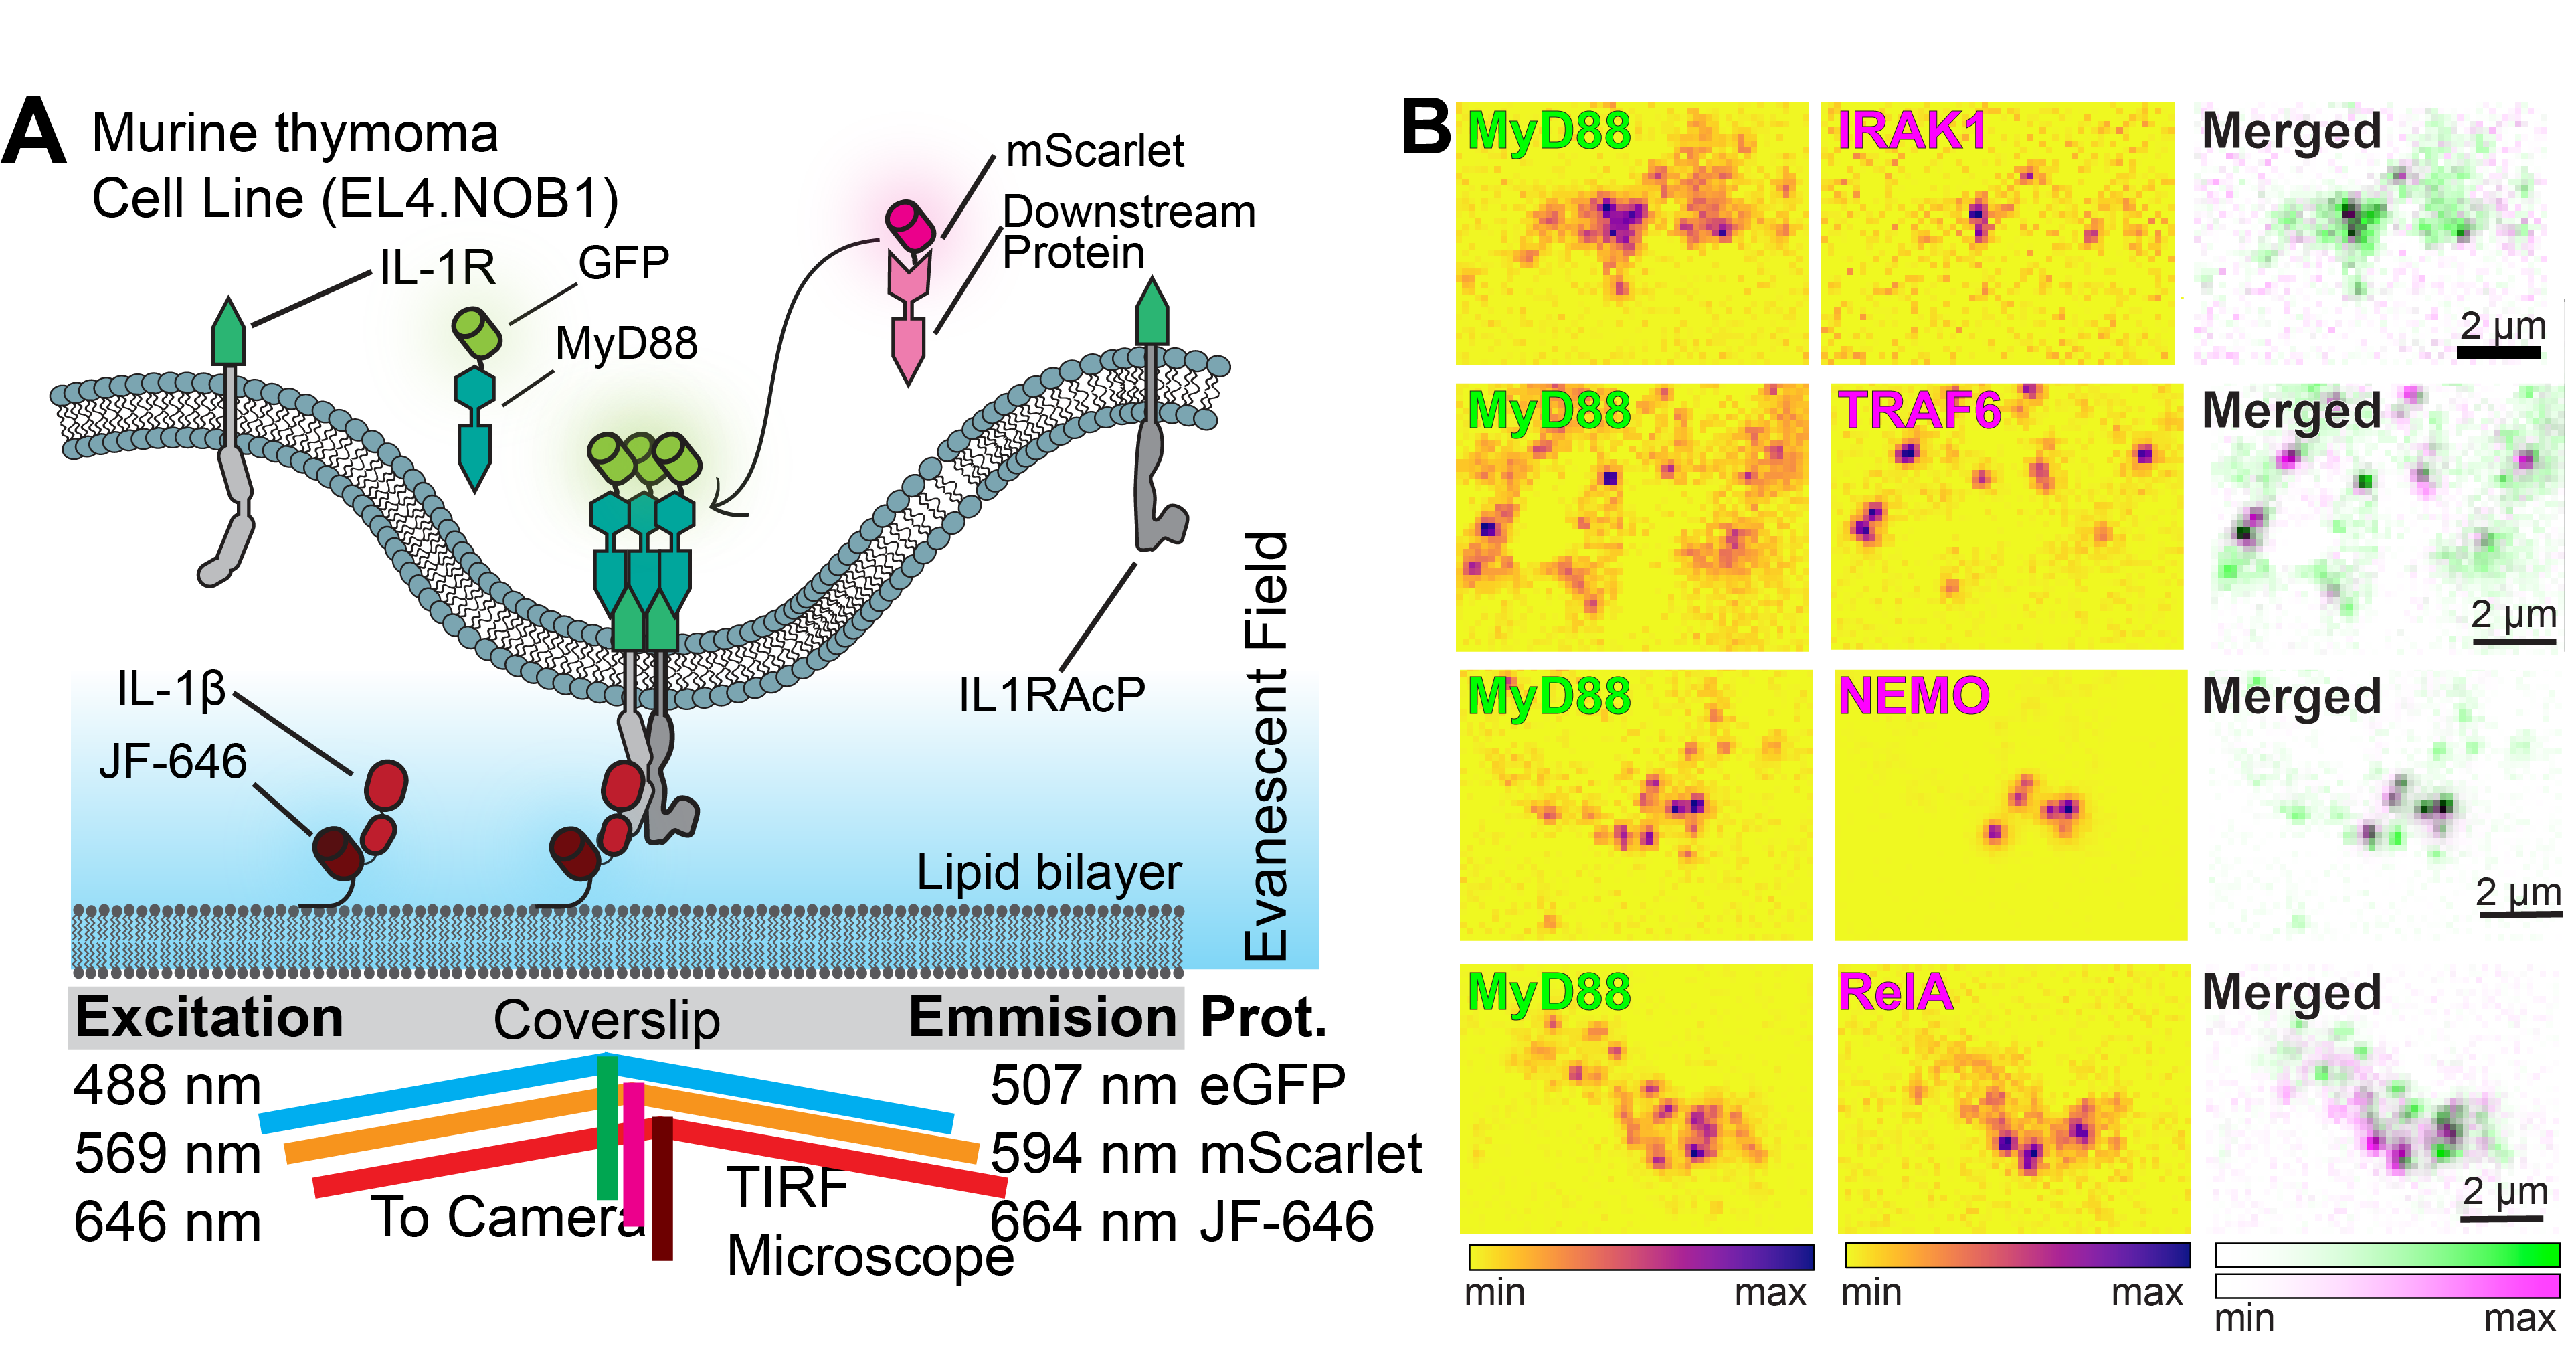
\includegraphics[width=\textwidth, height=\textheight, keepaspectratio]{mod/methods_used.png}}
\captionsetup{parbox=none}
\captionof{figure}[TIRF-M reveals key proteins in the Interleukin-1 pathway colocalize with MyD88-GFP]{\textbf{TIRF-M reveals key proteins in the Interleukin-1 pathway colocalize with MyD88-GFP.}
\\
\\
(A) Multi-color total internal reflection microscopy (TIRF-M) was used to image protein assembly dynamics. TIRF-M creates an evanescent field that allows studying receptor dynamics like in the IL-1R pathway. Proteins were tagged in pairs, with MyD88 as the reference and a downstream protein as the query. Cells were stimulated using a supported lipid bilayer functionalized with IL-1 for a controlled activation.
\\
\\
(B) MyD88 colocalized with all tagged downstream proteins. Images of MyD88 (left column) colocalizing with IRAK1, TRAF6, NEMO, and RelA (middle column) are shown. In the “Merged” image (right column), MyD88 appears in green, TRAF6 in magenta, colocalization in shades of black, and no protein in white. Scale bar, 2µm. Contrast was auto-adjusted by ImageJ. Color scale is provided at the bottom of the panels.
\\
\\
(Panel B is a modified version adapted from \autocite{Taylor_2017}. Panel B features imaging data provided by Fakun Cao, Niranjan Srikanth, Elba del Val, and Claudia Abad-Baucells, and were subsequently plotted by the thesis author.)}
\label{p2:system}
\end{centering}

To probe the dynamics of these signaling proteins, we used our assay (cell lines, imaging technique) as described before (Results~\ref{chapter:p1}, \autocite{Deliz-Aguirre_2021}, with improvements in the image analysis (Methods~\ref{chapter:PIRATES_PARLEYS}). To compare cell lines and establish a temporal order, proteins were tagged in pairs. Elke Ziska, Fakun Cao, Nichanok Auevechanickul, Claudia Abad-Baucells and Elba del Val Oriza fluorescently labeled the aforementioned proteins at the endogenous loci using CRISPR/Cas9. There was an upstream reference protein, MyD88, tagged with eGFP. The downstream proteins were tagged with mScarlet. Proteins were validated as described before. Then, labeled cells were imaged using TIRF-M. To quantify the dynamics, the images were processed with a pipeline that uses Python, ImageJ and R (Methods~\ref{chapter:PIRATES_PARLEYS}).

\section{The IL-1 pathway proteins assemble sequentially}
\label{section:IL1_seq}
\sectionmark{Sequential assembly}
Given the heterogeneous dynamics of different components colocalizing with MyD88, I first sought to quantitatively characterize the overall order, and the kinetics of the protein component assembly. The 32,598 puncta observed provide excellent grounds to perform quantitative analysis of the regulatory mechanisms governing the assembly and disassembly of IL-1 pathway proteins.

The Myddosome assembly sequence is MyD88, IRAK4 and IRAK1 \autocite{Lin_2010}\autocite{Deliz-Aguirre_2021}. But beyond the Myddosome, the IL-1 pathway assembly sequence is unknown. Literature surveys offer an untested hypothesis, that the assembly sequence is MyD88, IRAK4, IRAK1, TRAF6, TAB2, HOIL1, NEMO, RelA, and A20 \autocite{Cohen_2020}\autocite{Zarrin_2021}\autocite{Zinatizadeh_2021}, as shown in Fig.~\ref{img:pathway} and introduced in Section~\ref{section:downstream}. 

To obtain the average protein behavior, I measured the intensities of the corresponding channels in TIRF microscopy images (see section Methods~\ref{subsection:normalization} for normalization details). This is shown in Fig.~\ref{p2:1a}. In the x-axis is the puncta time since the tracking of the spot began, in the y-axis, its scaled intensity, and in color, the protein (more on these next). In Fig.~\ref{p2:1a}A, I explain the steps of the analysis. From left to right, I took the raw intensity time traces of all puncta in a cell line and constructed a median trace (second panel from left) by combining the trajectories of the median puncta at each timepoint. This resulted in a trace of intensity versus time that shows the behavior of the median at all times. Lastly (right panel), to compare across cell lines, the median curves were normalized from 0 to 1.\footnote{See Appendix~\ref{section:sequential} for rationale.} This normalization loses information about the relative intensities across cell lines, and cannot measure parallel assembly, but it allows a comparison of the timescales and important features of the assembly kinetics across cell lines (Fig.~\ref{p2:1a}, explanation on Appendix~\ref{section:sequential}).

Figure~\ref{p2:1a}B shows the experimental growth kinetics as time traces. The x-axis is the relative time since MyD88 nucleated to start the signal, and in the y-axis is the scaled intensity of the components. In the leftmost panel (Fig.~\ref{p2:1a}B), we can see that the two colored curves have distinct dynamics with IRAK4 (brown), IRAK1 (red) reaching mid-assembly at a similar time as MyD88 (black curve), while TRAF6 (orange), TAB2 (teal), HOIL1 (yellow), NEMO (green), A20 (light blue) and RelA (dark blue) reach mid-assembly after MyD88 (Figure~\ref{p2:1a}B).

This is the first evidence of the modular assembly of the IL-1 pathway (see Introduction~\ref{section:modularity}). An important finding arising from the quantitative imaging of assembly kinetics is that the IL-1 pathway proteins do not assemble all-at-once (see Introduction~\ref{subsection:assembly}), but rather, IL-1 pathway proteins assemble gradually, sequentially and seemingly into two protein modules. Overlaying all downstream protein time traces, we can observe that there is temporal organization, and identify a sequential assembly (Fig.~\ref{p2:1a}C). 


\begin{centering}
\centering{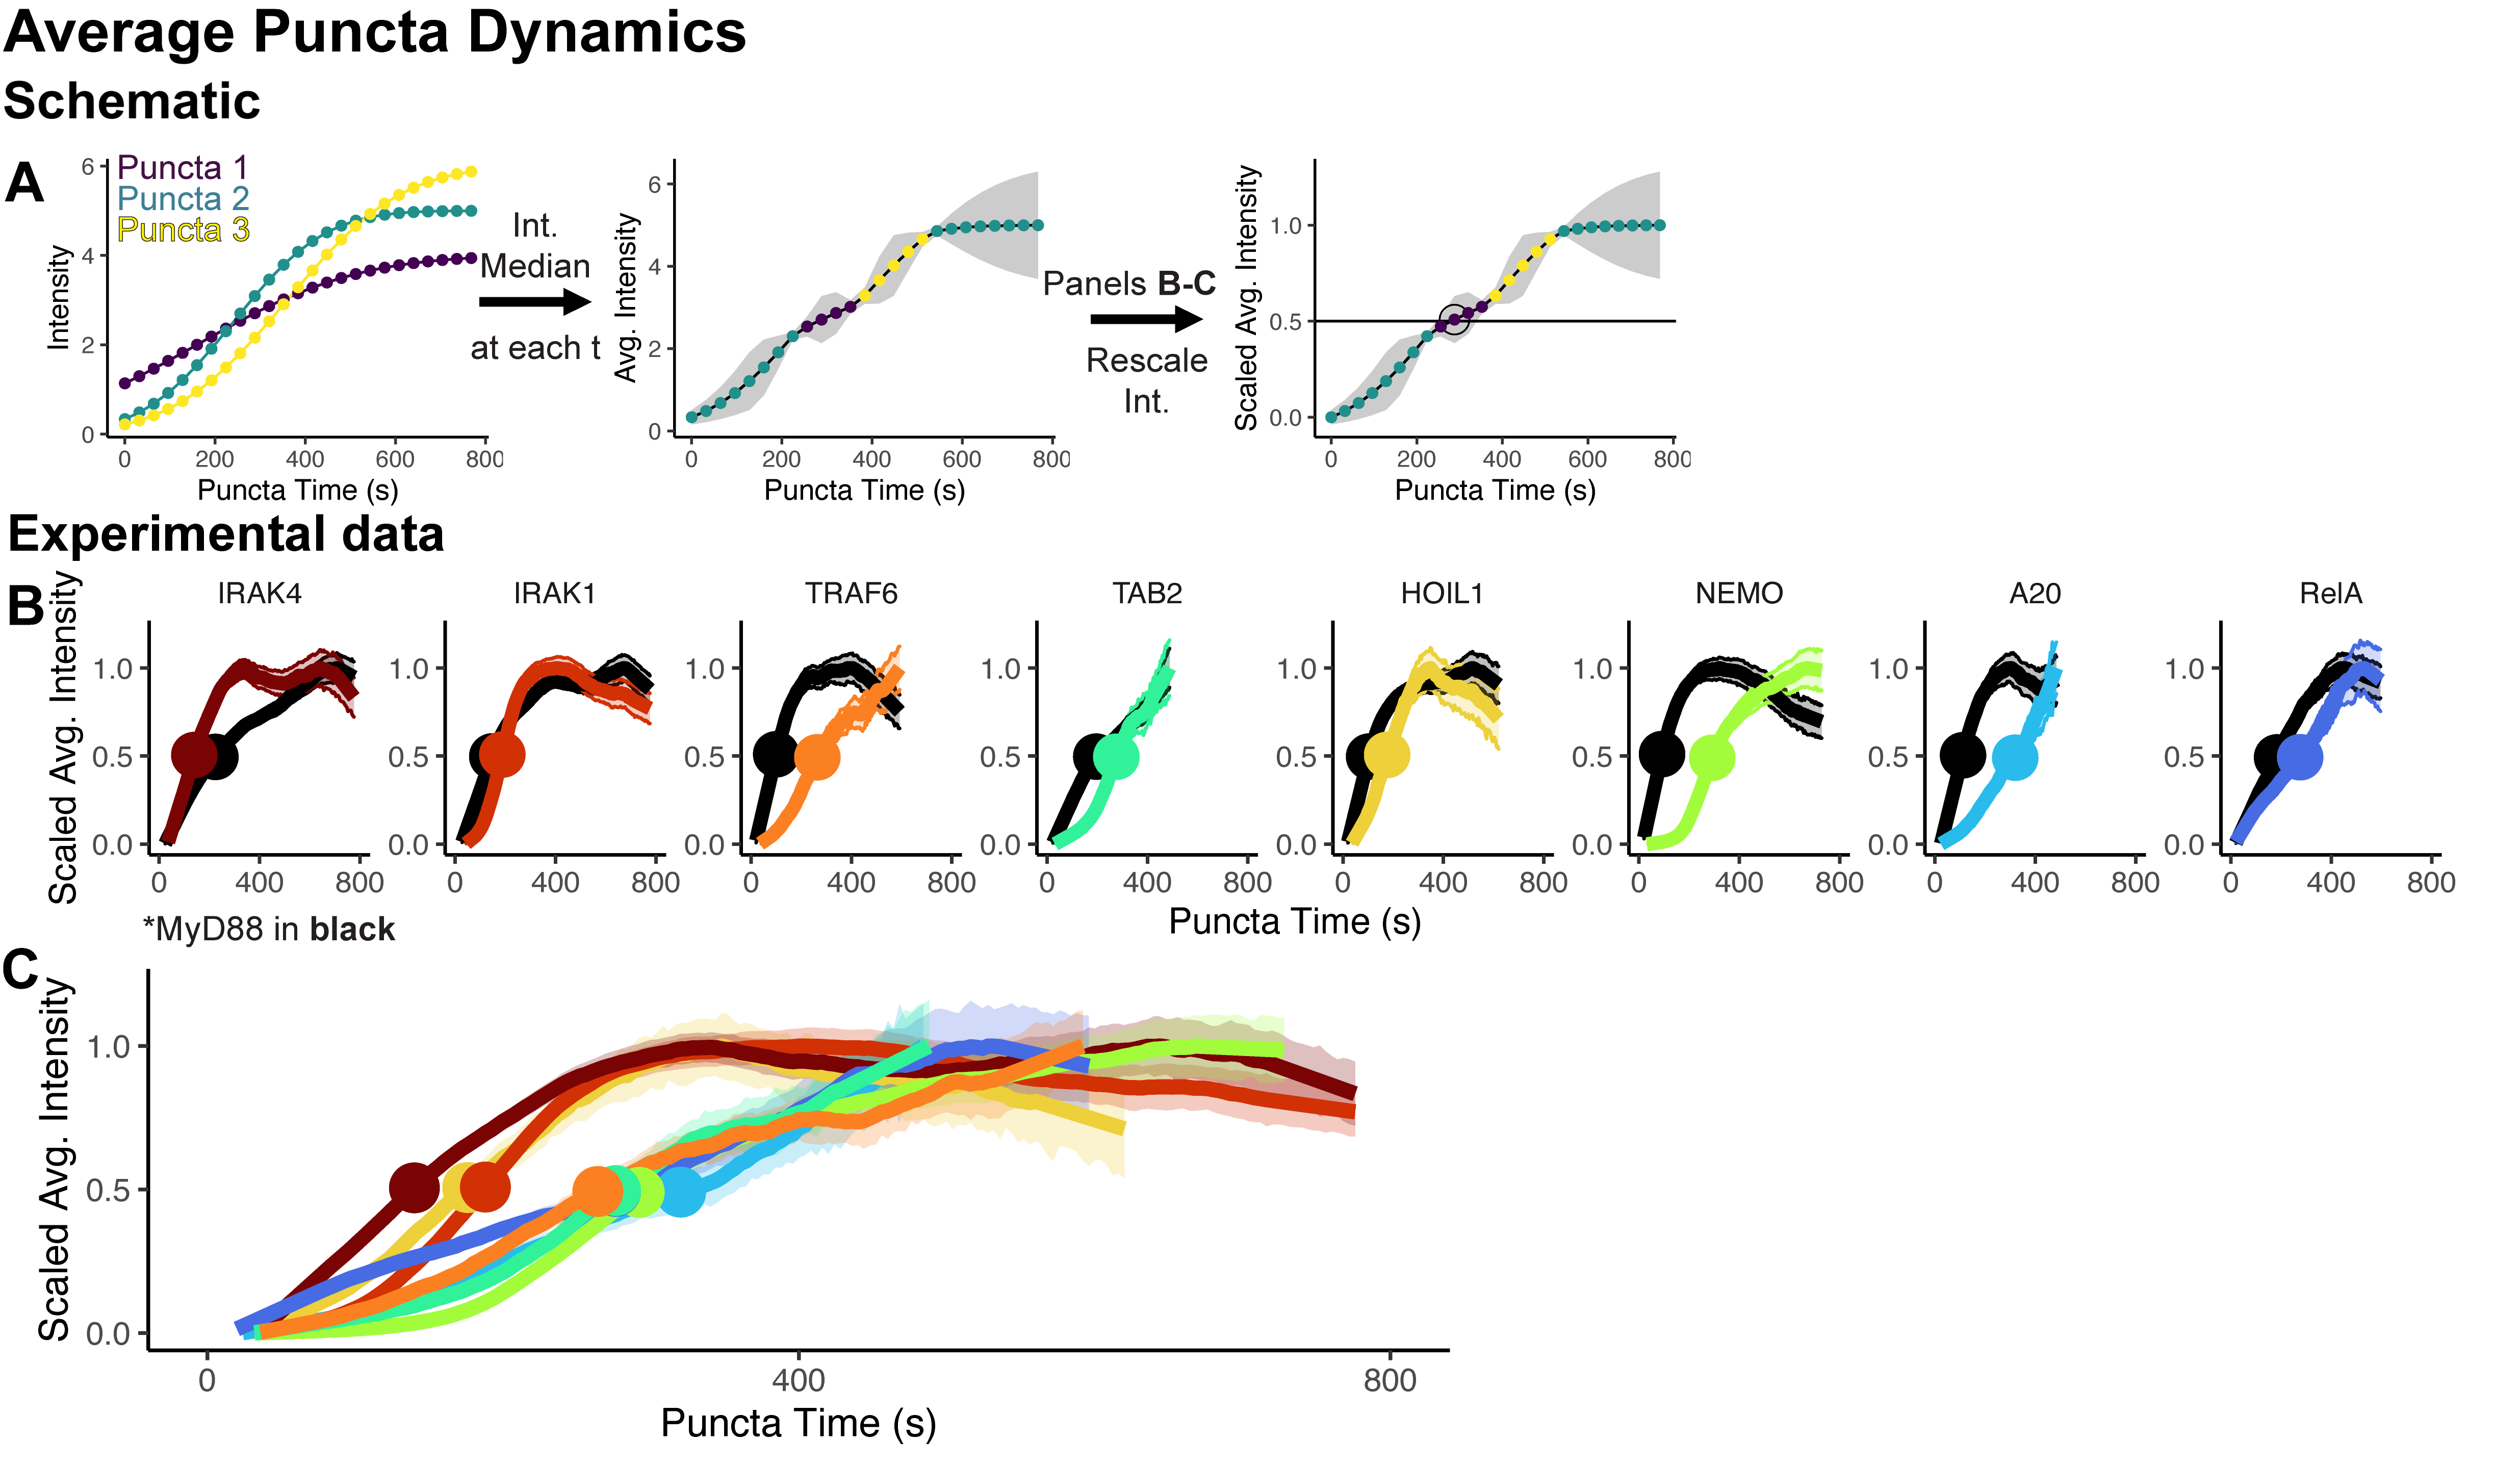
\includegraphics[height=\textwidth, width=\textheight, angle=-90, keepaspectratio]{mod/fig1a.png}}
\captionsetup{parbox=none}
\captionof{figure}[There is an oligomerization time delay between MyD88 and other proteins]{\textbf{There is an oligomerization time delay between MyD88 and other proteins.}
\\
\\
(A) To analyze the timing of assembly, median intensities were calculated for each timepoint. The standard error of the median is indicated by the shading. Curves were rescaled using min-max normalization for cell line comparison, with a peak brightness equal to 1 (panels E-F). The intensity midpoint (50\% max) was identified and represented as a dot in panels E-F, and converted to a bar plot in panel H. This reduces the bias to merging puncta.
\\
\\
(B) Time traces of different proteins show growth, with MyD88 in black and the downstream proteins in color. The dot indicates the mid-intensity point. N $\geq$ 125.
\\
\\
(C) Side-by-side time traces show a sequential protein assembly order, with the mid-intensity time marked by a dot.
\\
\\
(B-C: Imaging data provided by Fakun Cao, Niranjan Srikanth, Elba del Val, and Claudia Abad-Baucells, and were subsequently analyzed and plotted by the thesis author.)}
\label{p2:1a}
\end{centering}

In order to extract the assembly sequence from the data, I ranked the mid-assembly point of the time trace (Fig.~\ref{p2:1b}A, rationale on Appendix~\ref{section:sequential}). This offers an assembly sequence, shown in Figure~\ref{p2:1b}B, consistent with the literature \autocite{Lin_2010}\autocite{Deliz-Aguirre_2021}\autocite{Ye_2002}\autocite{Zarrin_2021}\autocite{Zinatizadeh_2021}, but differed with others in that HOIL1 assembles before TRAF6 \autocite{Cohen_2014}, TAB2 assembles before NEMO \autocite{Cohen_2020}, and RelA assembles before NEMO \autocite{Cohen_2020}\autocite{Zarrin_2021}\autocite{Zinatizadeh_2021}. The data suggested that the assembly sequence is MyD88, IRAK4, HOIL1, IRAK1, TRAF6, TAB2, RelA, NEMO, and A20 (Fig.~\ref{p2:1b}C).


\begin{centering}
\centering{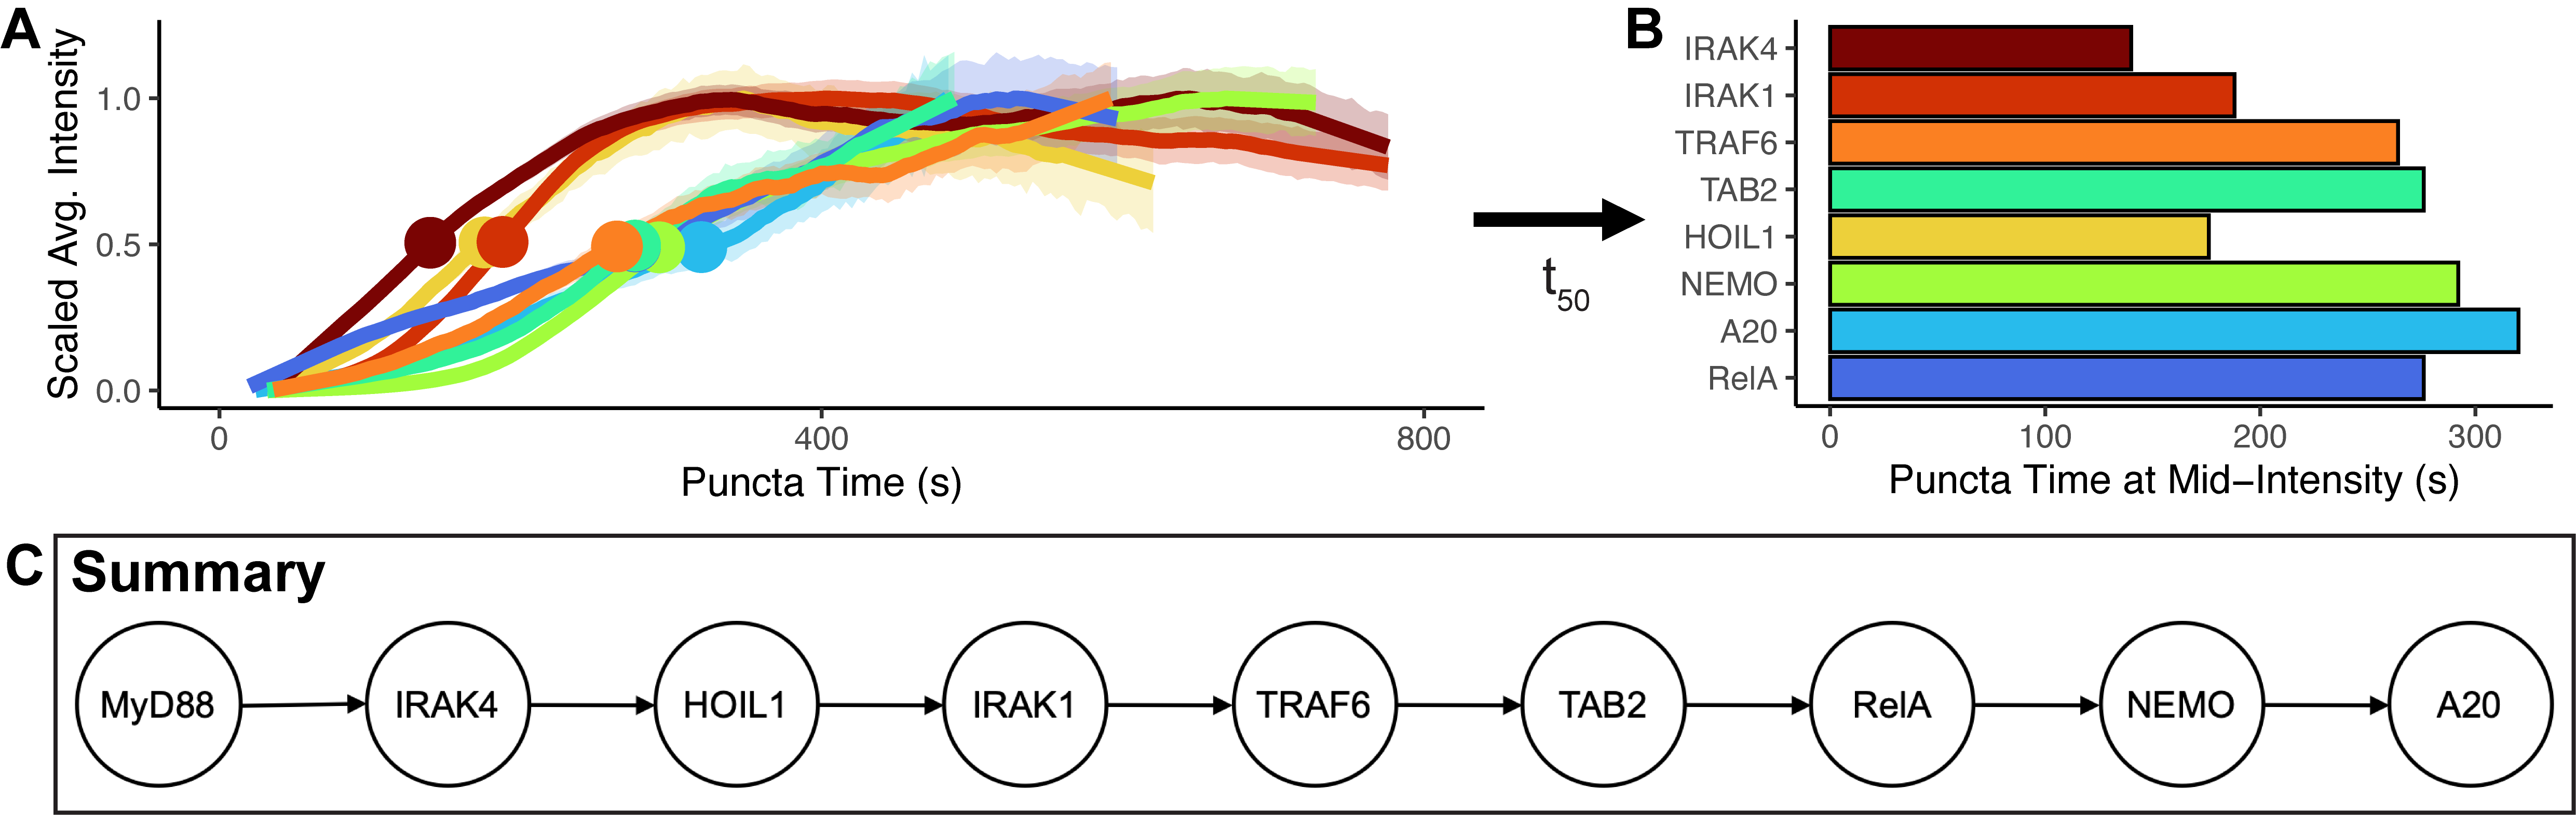
\includegraphics[height=\textwidth, width=\textheight, angle=-90, keepaspectratio]{mod/fig1b.png}}
\captionsetup{parbox=none}
\captionof{figure}[The Interleukin-1 pathway proteins assemble sequentially]{\textbf{The Interleukin-1 pathway proteins assemble sequentially.}
\\
\\
(A) Side-by-side time traces show a sequential protein assembly order, with the mid-intensity time marked by a dot.
\\
\\
(B) Median mid-intensity time per protein, indicating the assembly sequence as MyD88, IRAK4, HOIL1, IRAK1 , TRAF6, TAB2, RelA, NEMO, A20.
\\
\\
(C) Schematic of the assembly sequence.
\\
\\
(Panels A-B feature imaging data that was provided by Fakun Cao, Niranjan Srikanth, Elba del Val, and Claudia Abad-Baucells, and were subsequently analyzed and plotted by the thesis author.)}
\label{p2:1b}
\end{centering}

Taken together, I see a sequential assembly of downstream proteins starting with IRAK4 and ending with A20. The proteins assembled into condensed structures that are representative of the signaling pathway, and, importantly, the proteins show two classes of assembly kinetics. This provides our first hint that the IL-1 pathway assembly is not only sequential but also modular.

\section{Fluorescence recovery after photobleaching measurements reveal distinct chemical dynamics of the IL-1 pathway modules}
\label{section:biophysical}
\sectionmark{Chemical dynamics}
The assembly sequence of the proteins showed two distinct assembly timescales groups (Fig.~\ref{p2:1b}B). This hinted at the possibility that the IL-1 pathway uses modular organization (see Introduction~\ref{section:modularity} and Section~\ref{section:IL1_seq}). The literature suggests that different proteins in the IL-1 pathway have different structural properties. The Myddosome is a filamentous structure based on cryogenic electron microscope studies \autocite{Moncrieffe_2020}. The Myddosome has been observed to exhibit no turnover of its namesake protein, MyD88 \autocite{Deliz-Aguirre_2021}. Meanwhile, NEMO, a component of the IKK complex involved in the IL-1 pathway, has been visualized forming distinct punctate structures \autocite{Tarantino_2014}. I sought 

I sought to check if the distinct assembly kinetics of proteins (Results~\ref{section:IL1_seq}), truly represented distinct physical modules. To probe the biophysical properties of IL-1 pathway proteins, Fluorescence Recovery After Photobleaching (FRAP) analysis was used to elucidate protein exchange in the IL-1 pathway (refer to Appendix~\ref{section:biophysics} for the rationale). FRAP is a well-established experimental procedure that involves photobleaching all resident molecules in a structure or region and following the recovery of fluorescence within this structure or region as a proxy for exchange with the surrounding pool of unbleached molecules \autocite{Alberti_2019}.

The FRAP data plotted in Fig.~\ref{p2:2}A shows that following a drastic reduction in intensity at $t = 0$ (the photobleaching step) the intensity does not recover with time. This can also be seen in the zoomed snapshots of the Myddosome signalosome puncta below the graph of Fig.~\ref{p2:2}A. The results show that TRAF6-mScarlet puncta, similar to MyD88-eGFP (Results~\ref{chapter:p1}), exhibits no recovery after photobleaching (Fig.~\ref{p2:2}A). This finding suggests that TRAF6 forms stable, non-exchanging structures---consistent with the presumed nature of a static filament. Similar observations have been reported by the laboratory of Hao Wu where TRAF6 decorated CARMA1--BCL10--MALT1 filaments \autocite{David_2018}.

Following the same line of investigation, Fakun Cao performed FRAP analysis on HOIL1-mScarlet. Remarkably, unlike TRAF6, HOIL1 recovery occurred in less than a minute post-photobleaching (Fig.~\ref{p2:2}B), implying a dynamic exchange with the environment. This result may be interpreted in two possible ways: (1) HOIL1 might still be in the assembly phase, or (2) HOIL1 might be continually replacing itself. Given that the FRAP data of Fig.~\ref{p2:2}B was taken at 30 minutes post-stimulation, by which time the HOIL1 intensity is falling (Fig.~\ref{p2:2}B-C, yellow curves), I conclude that HOIL1 is likely showing dynamic exchange of molecules with the surrounding pool, unlike TRAF6 and other early Myddosome signalosome components.

With the FRAP data, we have a second independent and consistent evidence for modular architecture of the IL-1 pathway, consistent with the assembly kinetics. The protein components of the IL-1 pathway can therefore be classified into two modules, here termed the Myddosome signalosome and the NF-κB signalosome. I next explored the feedback dynamics between individual protein components to further test the modularity concept as introduced previously (see Introduction~\ref{section:modularity}).


\begin{centering}
\centering{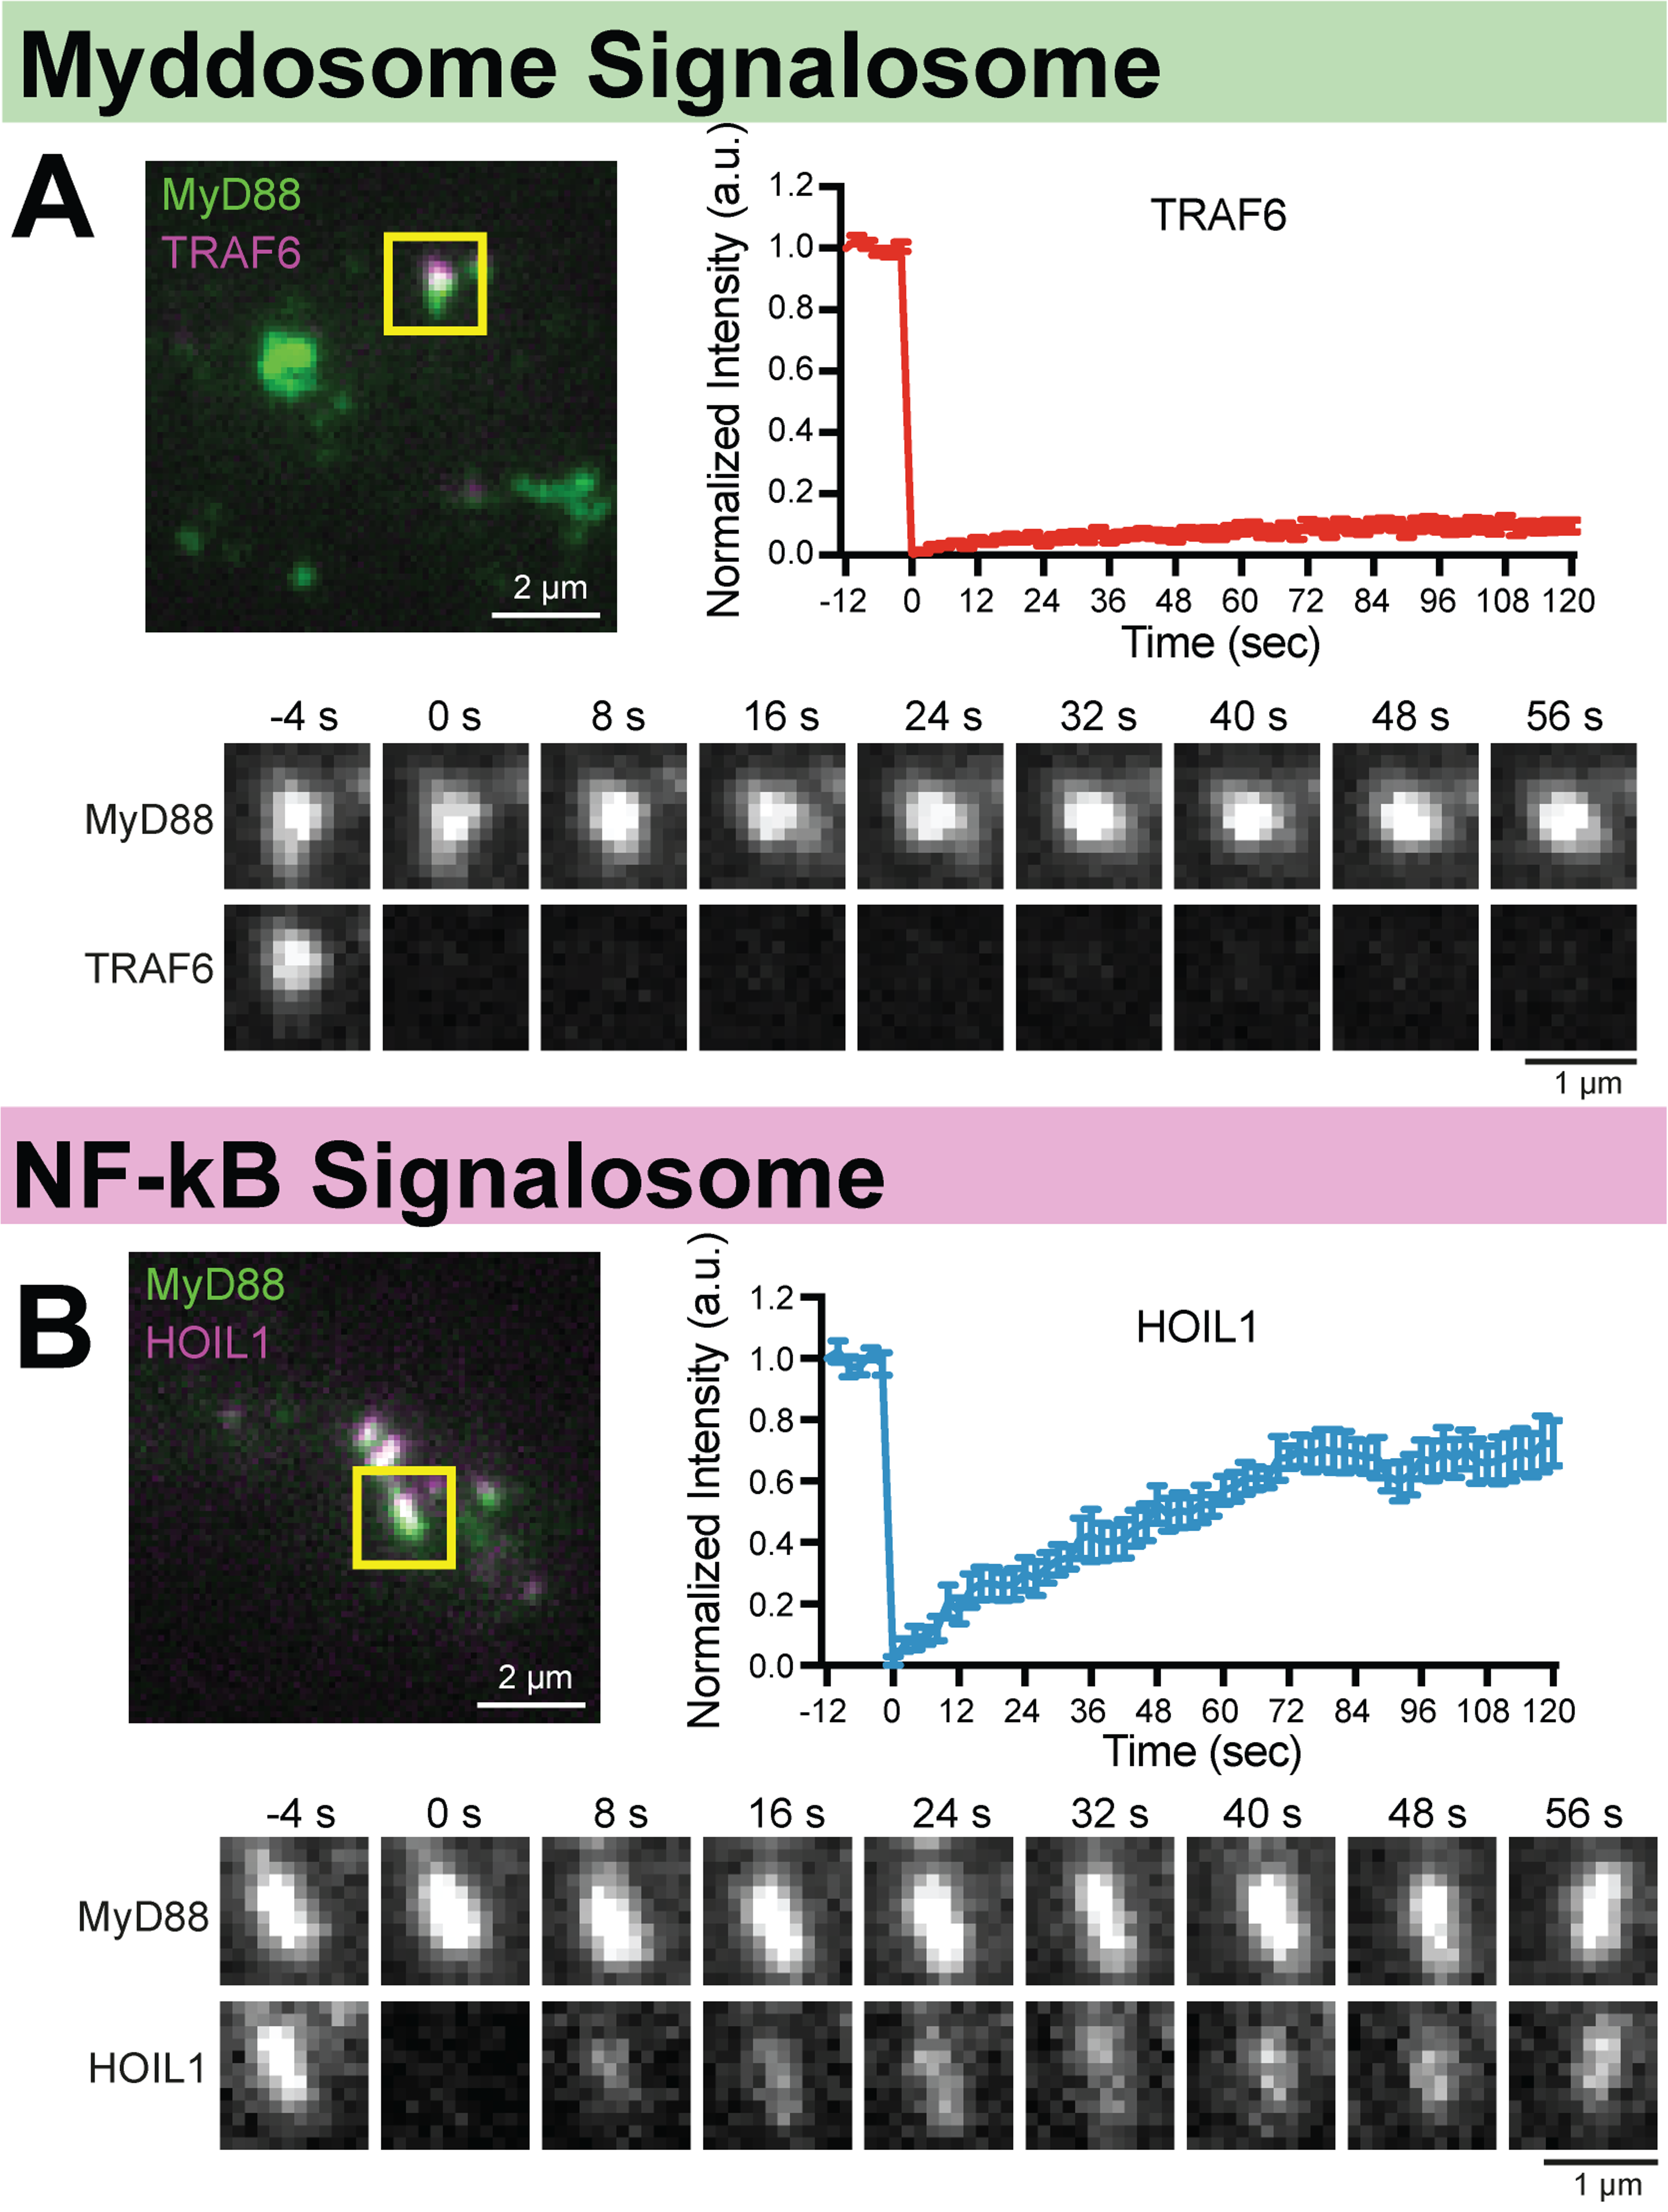
\includegraphics[width=0.75\textwidth, height=0.75\textheight, keepaspectratio]{mod/fig2.png}}

\captionsetup{parbox=none}
\captionof{figure}[IL-1 pathway proteins have distinct exchange dynamics]{\textbf{IL-1 pathway proteins have distinct exchange dynamics.}
\\
\\
(A-B) To investigate the exchange dynamics of the different signalosomes, I used fluorescence recovery after photobleaching (FRAP) analysis. Here, I examined whether the IL-1 pathway proteins have similar or distinct biophysical properties.
\\
\\
(A) TRAF6 does not recover after photobleaching.
\\
\\
(B) However, HOIL1 does show recovery after photobleaching,  suggesting it dynamically exchanges with the surrounding environment. This confirms that the assembly dynamics of the IL-1 pathway modules are different.
\\
\\
(A-B: Panels courtesy of Fakun Cao.)}
\label{p2:2}
\end{centering}

\section{Phase portrait analysis reveals two interactions dynamics between the two signalosomes}
\label{section:two_dynamics}
\sectionmark{Two dynamics}
Recently, phase portraits were used to uncover the actomyosin cortex assembly and disassembly dynamics by examining the colocalization dynamics of actin and WSP-1 \autocite{Yan_2022}. The phase portrait method allowed for the quantitative analysis of colocalization dynamics within any structure. Here, I adapted and applied this method to study the interactions between IL-1 pathway modules and rationalize the colocalization dynamics of the IL-1 pathway.\footnote{Phase portrait analysis is detailed in the Introduction~\ref{chapter:methods_applied}}. The procedure for building these phase portraits is outlined in Fig.~\ref{p2:3a} and Methods~\ref{section:pp_method}, with further explanations and hypotheses in Appendix~\ref{section:dynamics}.

In Fig.~\ref{p2:3}B-C, the x-axis measures the normalized intensity (stoichiometry) of MyD88 while the y-axis measures the normalized intensity (stoichiometry) of the query protein (B: IRAK1, C: RelA). Thus, every point in this graph corresponds to a particular internal composition (stoichiometry). At each internal composition, an arrow is plotted depicting the average (median) growth in MyD88 and IRAK1/RelA shown by all measured puncta with that composition.

Two main types of phase portraits were observed, with IRAK1 and RelA chosen as illustrative examples of the protein dynamics (Fig.~\ref{p2:3}, the rest are in Fig~\ref{p2:3b}). The phase portrait of IRAK1 depicts right arrows when no IRAK1 is present, which indicates MyD88 growth. When MyD88 size reached approximately 15\times, arrows turned up-right, suggesting potential merging of Myddosomes (Fig.~\ref{p2:3}B). It was noted that IRAK1 assembly occurred even in assemblies with a modest 3\times MyD88, indicating no discernible MyD88 size threshold for IRAK1.

The phase portrait of RelA, on the other hand, revealed a phase of MyD88 growth, then RelA growth, and finally, MyD88 shrink. Notably, RelA growth was evident even at 0-1.5\times MyD88, which aligns with the previously observed formation of RelA multimers at the plasma membrane (Fig.~\ref{p2:S1}D,~\ref{p2:S2}-~\ref{p2:S3}). At 12\times MyD88, RelA continues to grow but MyD88 disassembles. At 6\times RelA, MyD88 disassembly began. It also shows puncta have a maximum size of 15\times MyD88 and 15\times RelA. This pattern suggests potential size constraints for MyD88 and RelA.

Broadly, the two types of phase portraits are categorized as those exhibiting positive feedback (Fig.~\ref{p2:3}B) and those exhibiting negative feedback (Fig.~\ref{p2:3}C). A complete collection of phase portraits can be found in the Appendix~\ref{section:dynamics} and Fig.~\ref{p2:3b}. Proteins IRAK4, IRAK1, TRAF6, and TAB2 demonstrated positive feedback (Fig.~\ref{p2:3b}A), while NEMO, HOIL1, A20, and RelA showed negative feedback (Fig.~\ref{p2:3b}B). Interestingly, the feedback dynamics correlate with both the assembly time kinetics (Results~\ref{section:biophysical}, Fig.~\ref{p2:1b}) and the FRAP analysis (Results~\ref{section:biophysical}, Fig.~\ref{p2:2}). To summarize, the positive feedback proteins (IRAK4, IRAK1, TRAF6, and TAB2) assembled first and showed no recovery after photobleaching, while the negative feedback proteins (NEMO, HOIL1, A20, and RelA) assembled later, and did show fluorescence recovery after photobleaching.

Taken together, these three independent (assembly kinetics, FRAP and phase portraits) clearly agree both on the existence of two modules in the IL-1 pathway, and on the categorization of proteins into two modules. Therefore, I propose the terms “Myddosome signalosome” to refer to the assembly containing the Myddosome (MyD88, IRAK4, IRAK1) plus TRAF6 and TAB2, and “NF-κB signalosome” for the second assembly here defined as containing HOIL1, NEMO, RelA and A20 (Fig.~\ref{p2:3}D). Next, different time cutoffs were used to illustrate dynamics over time as phase portraits do not inherently show time.


\begin{centering}
\centering{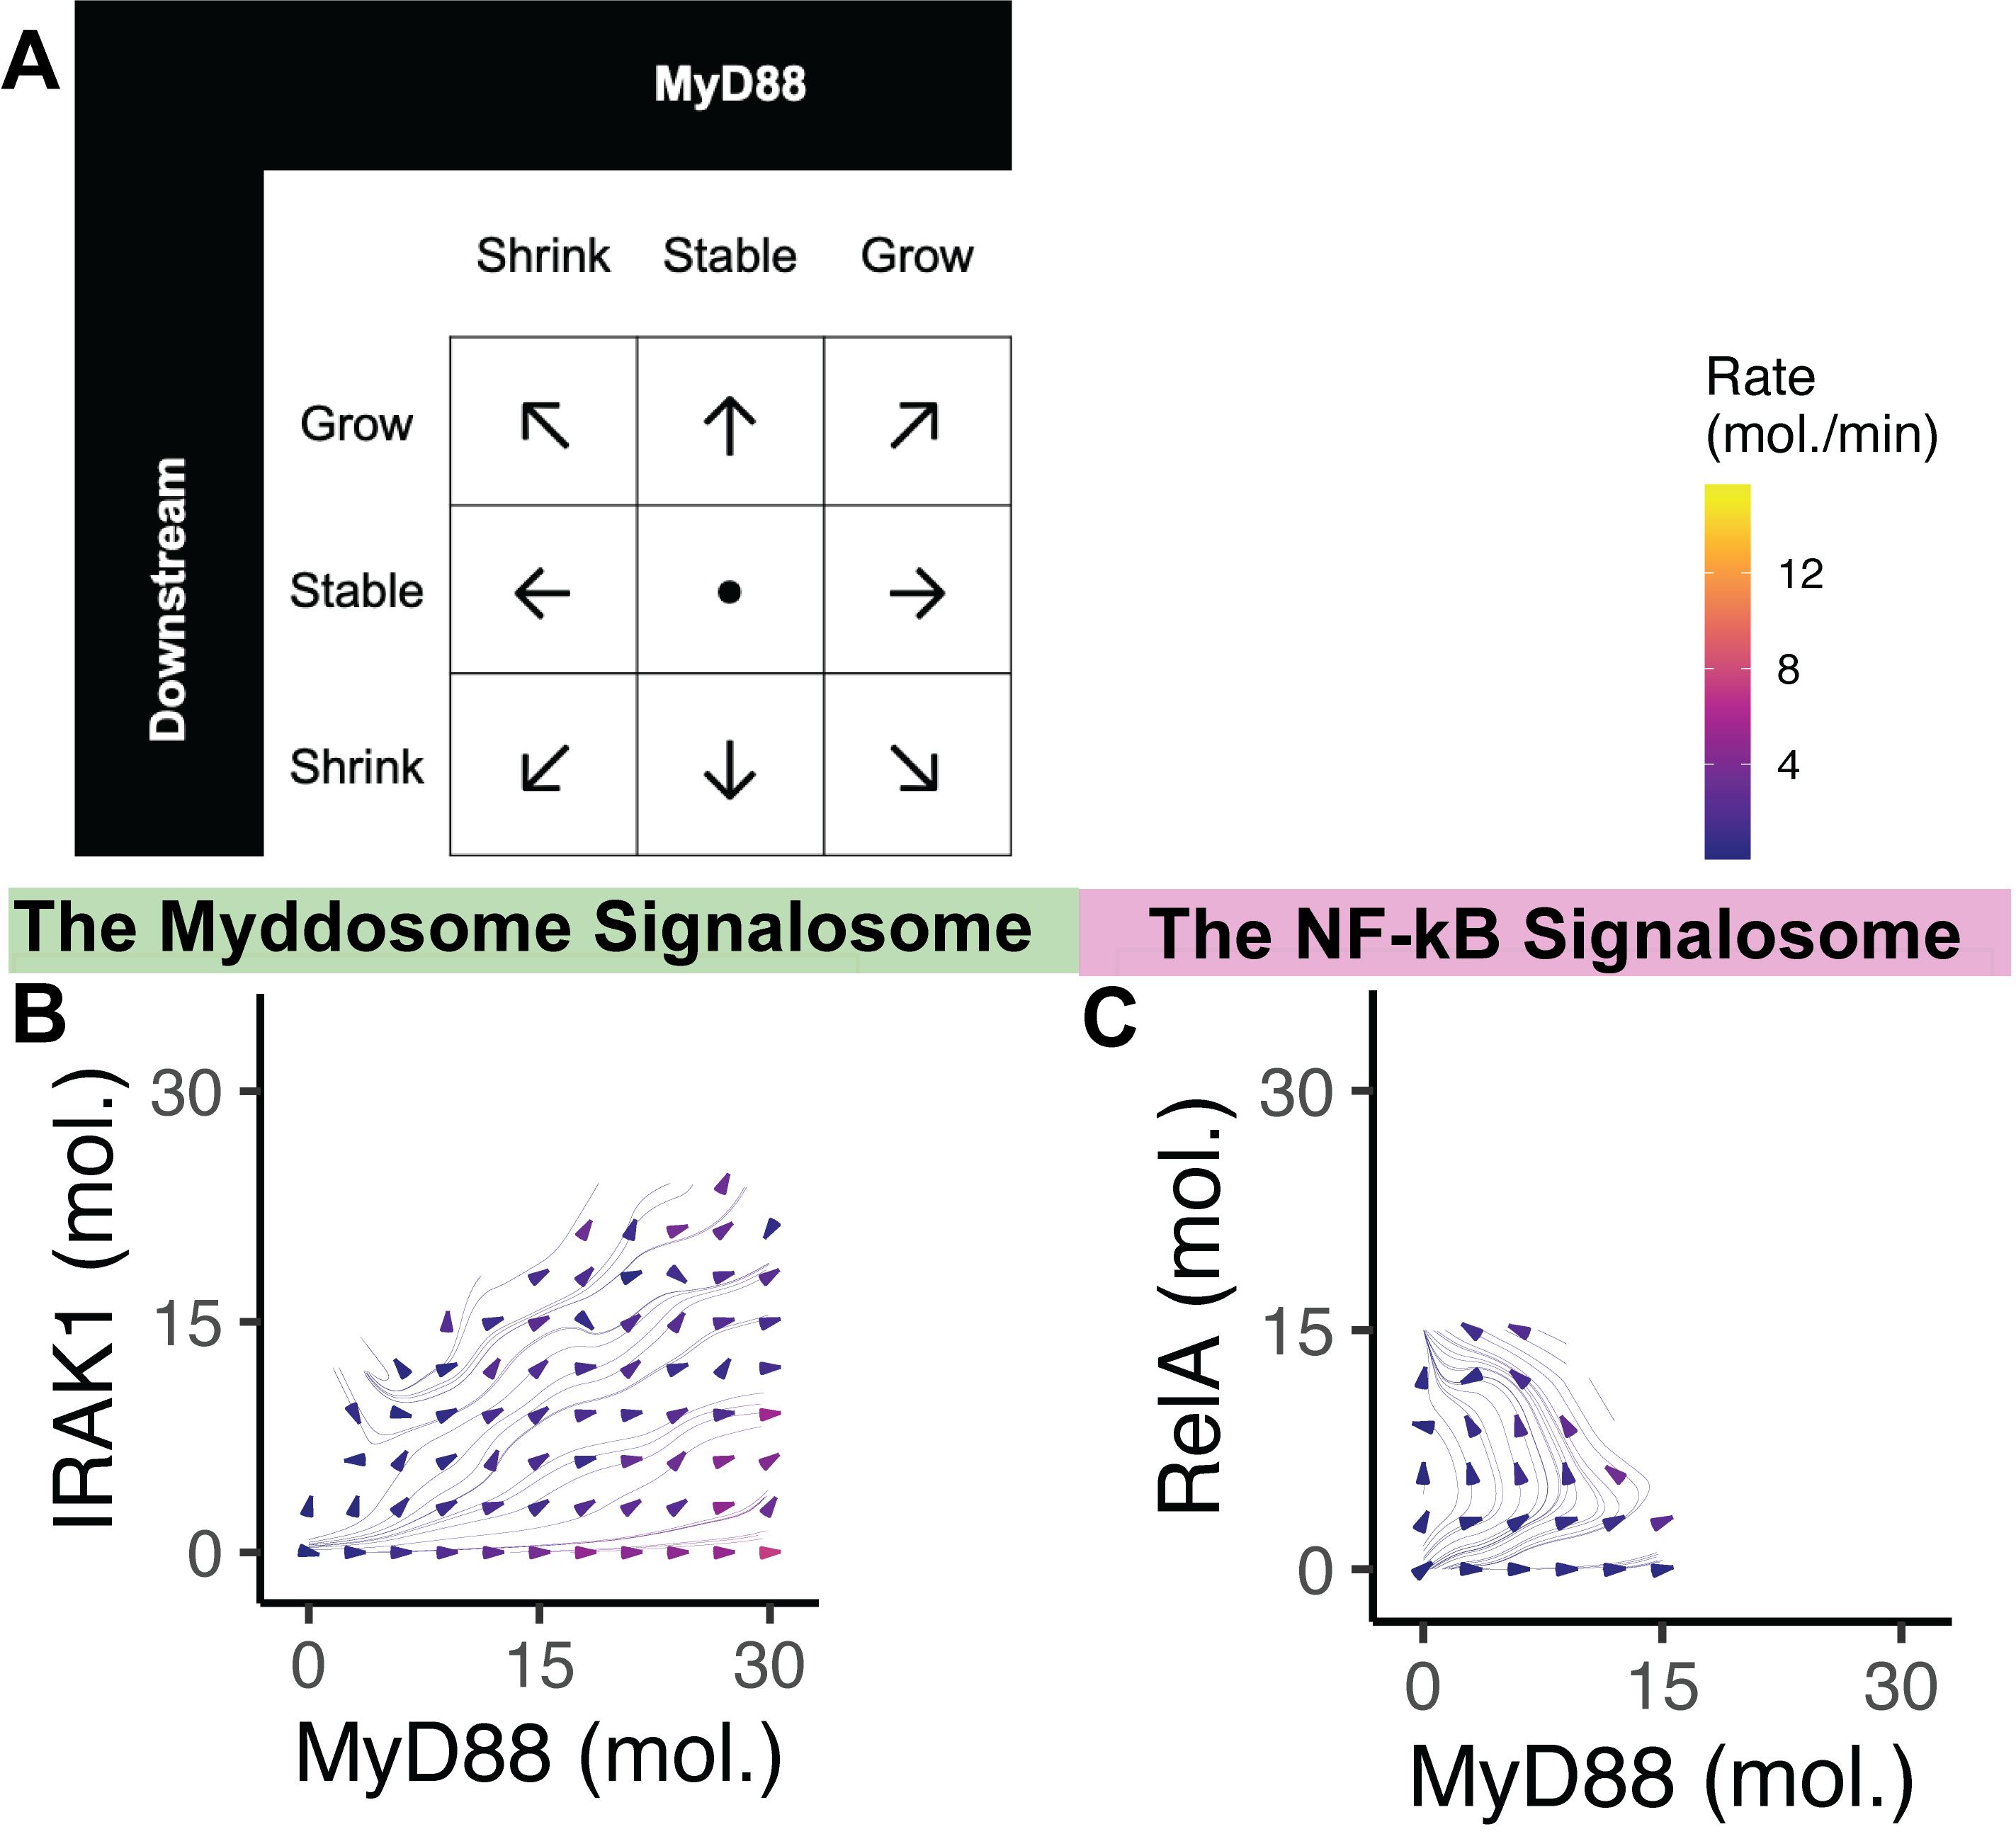
\includegraphics[width=\textwidth, height=\textheight, keepaspectratio]{mod/fig3.png}}

\captionsetup{parbox=none}
\captionof{figure}[There are at least two signalosomes in the IL-1 pathway as revealed by phase portrait analysis]{\textbf{There are at least two signalosomes in the IL-1 pathway as revealed by phase portrait analysis.} 
\\
\\
(A) Arrow angles indicate protein growth or disassembly. A right-pointing arrow signifies MyD88 growth, while an upward arrow indicates downstream protein growth. Conversely, a bottom-left-pointing arrow implies disassembly of both proteins. The arrow angle is calculated using the two-argument tangent (atan2) of the downstream protein and MyD88 change in intensity. Further details on this calculation can be found in Methods~\ref{chapter:PIRATES_PARLEYS}.
\\
\\
(B) Phase portraits of IRAK4, IRAK1, TRAF6, and TAB2 display positive feedback with up-right-pointing arrows.
\\
\\
(C) Phase portraits of NEMO, HOIL1, A20, and RelA exhibit a center-like (“circular”) pattern, indicating sequential MyD88 growth, downstream protein growth, and ultimately, MyD88 disassembly. This pattern is interpreted as negative feedback.
\\
\\
(B-C) Overall, there are two primary categories of phase portraits: positive and negative feedback. These phase portraits suggest the existence of two signalosomes in the IL-1 pathway: the Myddosome signalosome (positive feedback) and the NF-κB signalosome (negative feedback).
\\
\\
(B: Imaging data courtesy of Niranjan Srikanth, Fakun Cao. C: Imaging data courtesy of Claudia Abad-Baucells. Analysis, plots by the thesis author.)}
\label{p2:3}
\end{centering}

Further investigation into the temporal dynamics of these protein assemblies was undertaken. The Myddosome dynamics showed positive feedback (Fig.~\ref{p2:S4}A) in two stages: (i) MyD88 growth and (ii) downstream Myddosome signalosome protein growth (Fig.~\ref{p2:S4}B). All Myddosome signalosome proteins showed comparable dynamics.

Using IRAK1 as an example, its dynamics revealed that MyD88 growth precedes IRAK1 at 200 seconds. IRAK1 was preferentially recruited to 9\times MyD88 assemblies, but with some size tolerance that widened over time. The most rapid MyD88 growth occurred within 400 seconds following the appearance of the first spot. Arrows pointed in various directions, suggesting a potential disassembly or equilibrium state after 800 seconds (Fig.~\ref{p2:4}A). While potential size thresholds may exist, the related information seems to diminish over time, possibly as a result of puncta merging.

The NF-κB signalosome dynamics were similar to Myddosome signalosome proteins in that there is an initial positive feedback, but at later timepoints, the NF-κB signalosome proteins produce negative feedback with MyD88 (Fig.~\ref{p2:S4}B).

Using RelA as an example, the RelA phase portraits showed primarily MyD88 growth with some RelA trimers present within the first 200 seconds, though these trimers exhibited negligible growth. RelA binding was observed at 400 seconds (Fig.~\ref{p2:4}C). At 600 seconds, large RelA assemblies triggered MyD88 disassembly (Fig.~\ref{p2:4}C). Thus, the NF-κB signalosome has an additional stage: (iii) MyD88 disassembly (Fig.~\ref{p2:4}D). These feedback dependencies are quantitatively explored in Appendix~\ref{section:phase_lines})

So far, I have described the average growth dynamics of protein pairs as IL-1 pathway protein puncta change composition. In order to quantitatively extract quantitative information about the relationship between MyD88 growth and the downstream protein oligomer size, I calculated a single number to capture the relationship between the two, positive numbers being a positive correlation between the two (positive feedback), and a negative number means negative correlation which would mean negative feedback.


\begin{centering}
\centering{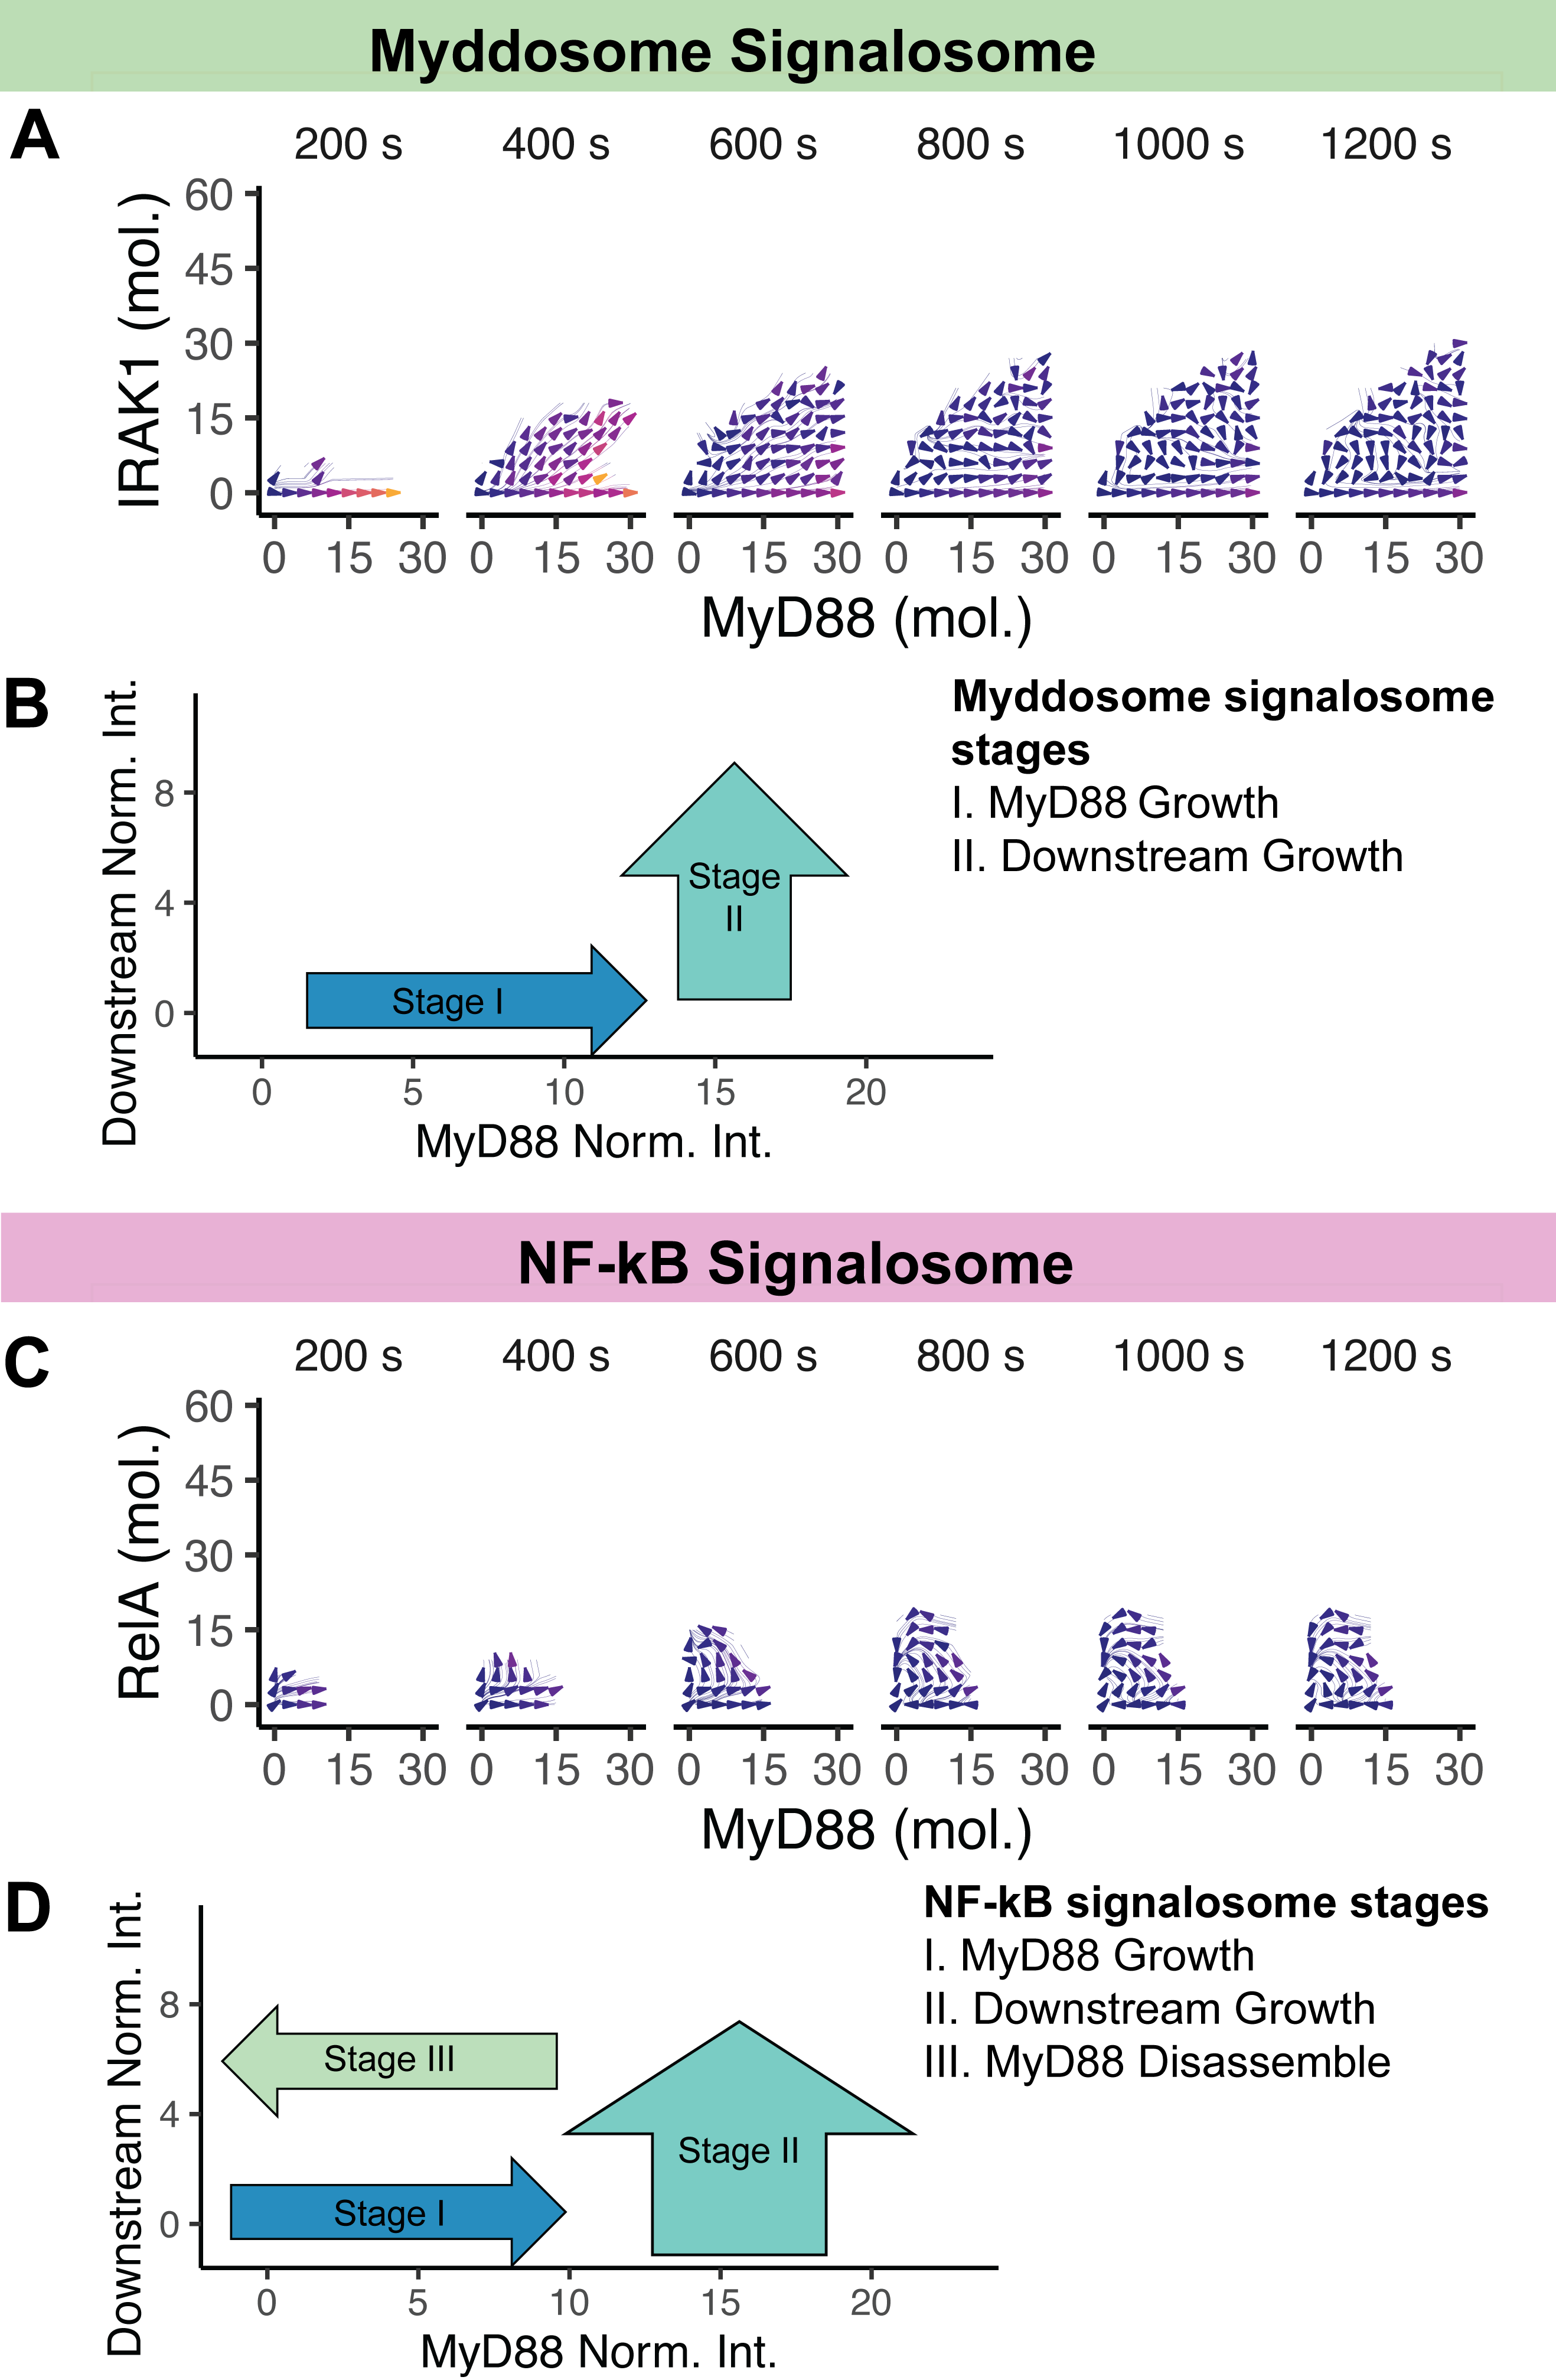
\includegraphics[width=\textwidth, height=\textheight, keepaspectratio]{mod/fig4.png}}

\captionsetup{parbox=none}
\captionof{figure}[The IL-1 pathway signalosomes have assembly stages evident in their distinct temporal dynamics]{\textbf{The IL-1 pathway signalosomes have assembly stages evident in their distinct temporal dynamics.}
\\
\\
(A, C) Phase portraits with distinct timepoint cutoffs (facets), with each timepoint indicating the time elapsed since the appearance of the first spot.
\\
\\
(A) The Myddosome signalosome forms within the initial 400 seconds (post first punctum), suggesting the early formation of the Myddosome module.
\\
\\
(B, D) Phase portraits can be employed to identify stages in protein assembly.
\\
\\
(B) The Myddosome signalosome displays initial MyD88 growth (right-pointing arrows, 200 seconds) and subsequent recruitment of Myddosome signalosome downstream proteins (IRAK4, IRAK1, TRAF6, TAB2) (upward-pointing arrows, 400 seconds).
\\
\\
(C) The NF-κB signalosome forms later, around 600 seconds, with MyD88 binding first followed by the recruitment of HOIL1, NEMO, RelA, and ultimately, A20. The NEMO phase portraits indicate that not all large MyD88 assemblies recruit NEMO, suggesting potential binding to a different pathway.
\\
\\
(D) The NF-κB signalosome (NEMO, HOIL1, RelA, A20) exhibits similar dynamics of MyD88 assembly (right-pointing arrows), and downstream protein assembly (upward-pointing arrows) but also demonstrates MyD88 disassembly (left-pointing arrows, 800 seconds).
\\
\\
(E) The phase portrait analysis revealed that there are assembly steps where assemblies grow larger over time. Larger Myddosome signalosome assemblies then recruit the NF-κB signalosome. The appearance of the NF-κB signalosome triggers the disassembly of MyD88.
\\
\\
(A, C: Imaging data courtesy of Fakun Cao, Niranjan Srikanth, Elba del Val and Claudia Abad-Baucells. Analysis, plots by the thesis author.)}
\label{p2:4}
\end{centering}

\section{Modules can be recapitulated with a single value}
\sectionmark{Single value for modules}
\label{section:single_value}
\sectionmark{Single value for modules}
From systems biology of the cell to the evolution of organisms, modularity is common across biological scales \autocite{Sadowski_1986}. Here, the assembly kinetics show the presence of two modules in the IL-1 pathway (Fig.~\ref{p2:1b}), the FRAP data shows the different material properties of these two modules (Fig.~\ref{p2:2}), and the phase portrait analysis shows the feedback between these modules (Fig.~\ref{p2:3}). While the feedback is visualized in the phase portraits, to confirm that the three methods agree on the division of proteins between the modules, I calculated a single metric from the phase portraits. More specifically, to synthesize the information, I applied dimensionality reduction of the phase lines (detailed definition in Appendix~\ref{section:thresholds}). I correlated MyD88 kinetics with the oligomer size (that is, stoichiometry) of downstream proteins using the Pearson correlation coefficient (R), see Fig.~\ref{p2:5b}.

The observations indicate that MyD88 kinetics have a positive correlation with the Myddosome signalosome protein components. This means that for Myddosome signalosome components, the larger the oligomer size, the faster MyD88 grows, and for NF-κB signalosome components, the larger the oligomer, the faster it disassembles. The strength of the correlation was consistent with the assembly sequence (Fig.~\ref{p2:5b}A), strengthening support that the IL-1 pathway has two distinct signalosomes (Fig.~\ref{p2:5b}). The two signalsomes proposed previously, the Myddosome signalosome and the NF-κB signalosome, can now be seen to consist of: (Myddosome signalosome) MyD88, IRAK4, IRAK1, TRAF6, and TAB2, and (NF-κB signalosome) NEMO, HOIL1, A20, and RelA, respectively. This study provides a foundation for further research to confirm these findings and explore the implications for understanding and manipulating these biochemical circuits.


\begin{centering}
\centering{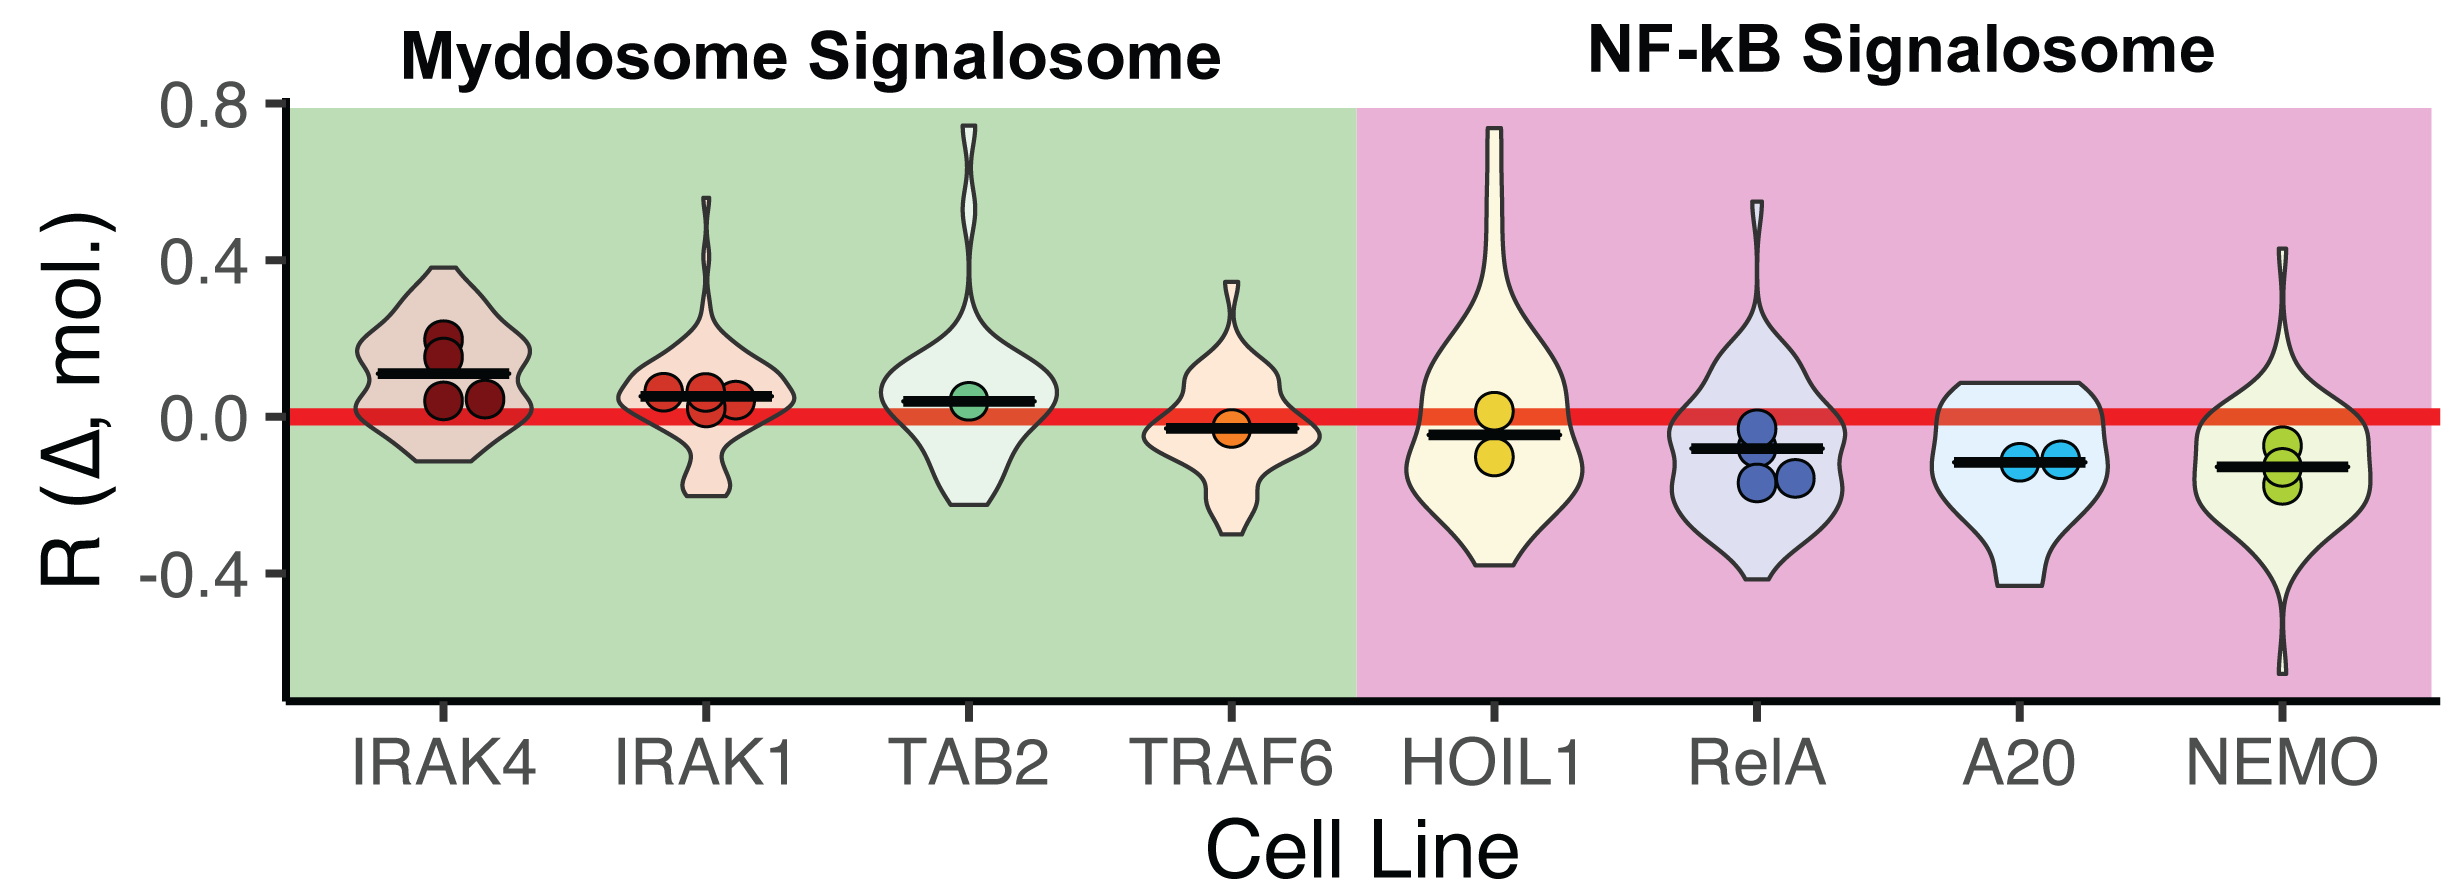
\includegraphics[width=\textwidth, height=\textheight, keepaspectratio]{mod/fig5b.png}}
\captionsetup{parbox=none}
\captionof{figure}[The IL-1 pathway signalosome dynamics can be recapitulated with a single numerical value]{\textbf{The IL-1 pathway signalosome dynamics can be recapitulated with a single numerical value.} The dynamic behavior of IL-1 pathway signalosomes can be simplified using correlations. This enables the reduction of complex signalosome dynamics down to a single numerical value. I calculated the Pearson correlation coefficient between MyD88 growth and downstream protein size. This reduces the number of dimensions to one number to indicate whether there is a positive or negative relationship between MyD88 growth and the downstream protein. Examining the correlation coefficients, IRAK4, IRAK1, and TAB2 exhibited clear positive feedback, with TRAF6 being borderline. These are part of the Myddosome signalosome. HOIL1, RelA, A20, and NEMO showed negative correlation, with HOIL1 being borderline. The rank of correlation coefficients roughly correlates with the assembly order. Each circle represents an image replicate. The bar indicates the median correlation. Violin plot uses the puncta data. (Imaging data courtesy of Fakun Cao, Niranjan Srikanth, Elba del Val and Claudia Abad-Baucells. Analysis, plots by the thesis author.)}
\label{p2:5b}
\end{centering}

\section{The NF-κB module triggers the disassembly of the Myddosome module}
\label{section:disassembly_results}
\sectionmark{Disassembly}
Thus far, I have employed MyD88 as a reference protein, comparing its growth performance to downstream proteins (the “query proteins”). If the IL-1 pathway is indeed modular, with similar protein functions within signalosomes, I anticipate that any protein from the Myddosome signalosome compared to any protein in the NF-κB signalosome will display similar dynamics.

Given that eGFP is prone to bleaching, it seems reasonable to expect improved temporal resolution from using a more downstream reference protein. Such a protein should also better resolve events occurring later in the timeline. Consequently, I shifted the reference protein from MyD88 to TRAF6. A TRAF6-eGFP NEMO-mScarlet cell line was developed to facilitate this inquiry. The resulting phase portrait, however, could take several forms. The unpredictability lies primarily in whether IL-1 pathway proteins disassemble or not.

The kymographs revealed an interesting sequence: TRAF6 puncta appeared first, followed by NEMO recruitment to the same puncta. Intriguingly, while TRAF6 disappeared, NEMO persisted, indicating that the NF-κB signalosome remains at the plasma membrane (Fig.~\ref{p2:6a}). This implies that the previously shown negative feedback (Figs.~\ref{p2:3}-~\ref{p2:5b},~\ref{p2:S5}) is perhaps the Myddosome signalosome disassembling. Next, I will apply phase portrait analysis to uncover the TRAF6-NEMO dynamics.


\begin{centering}
\centering{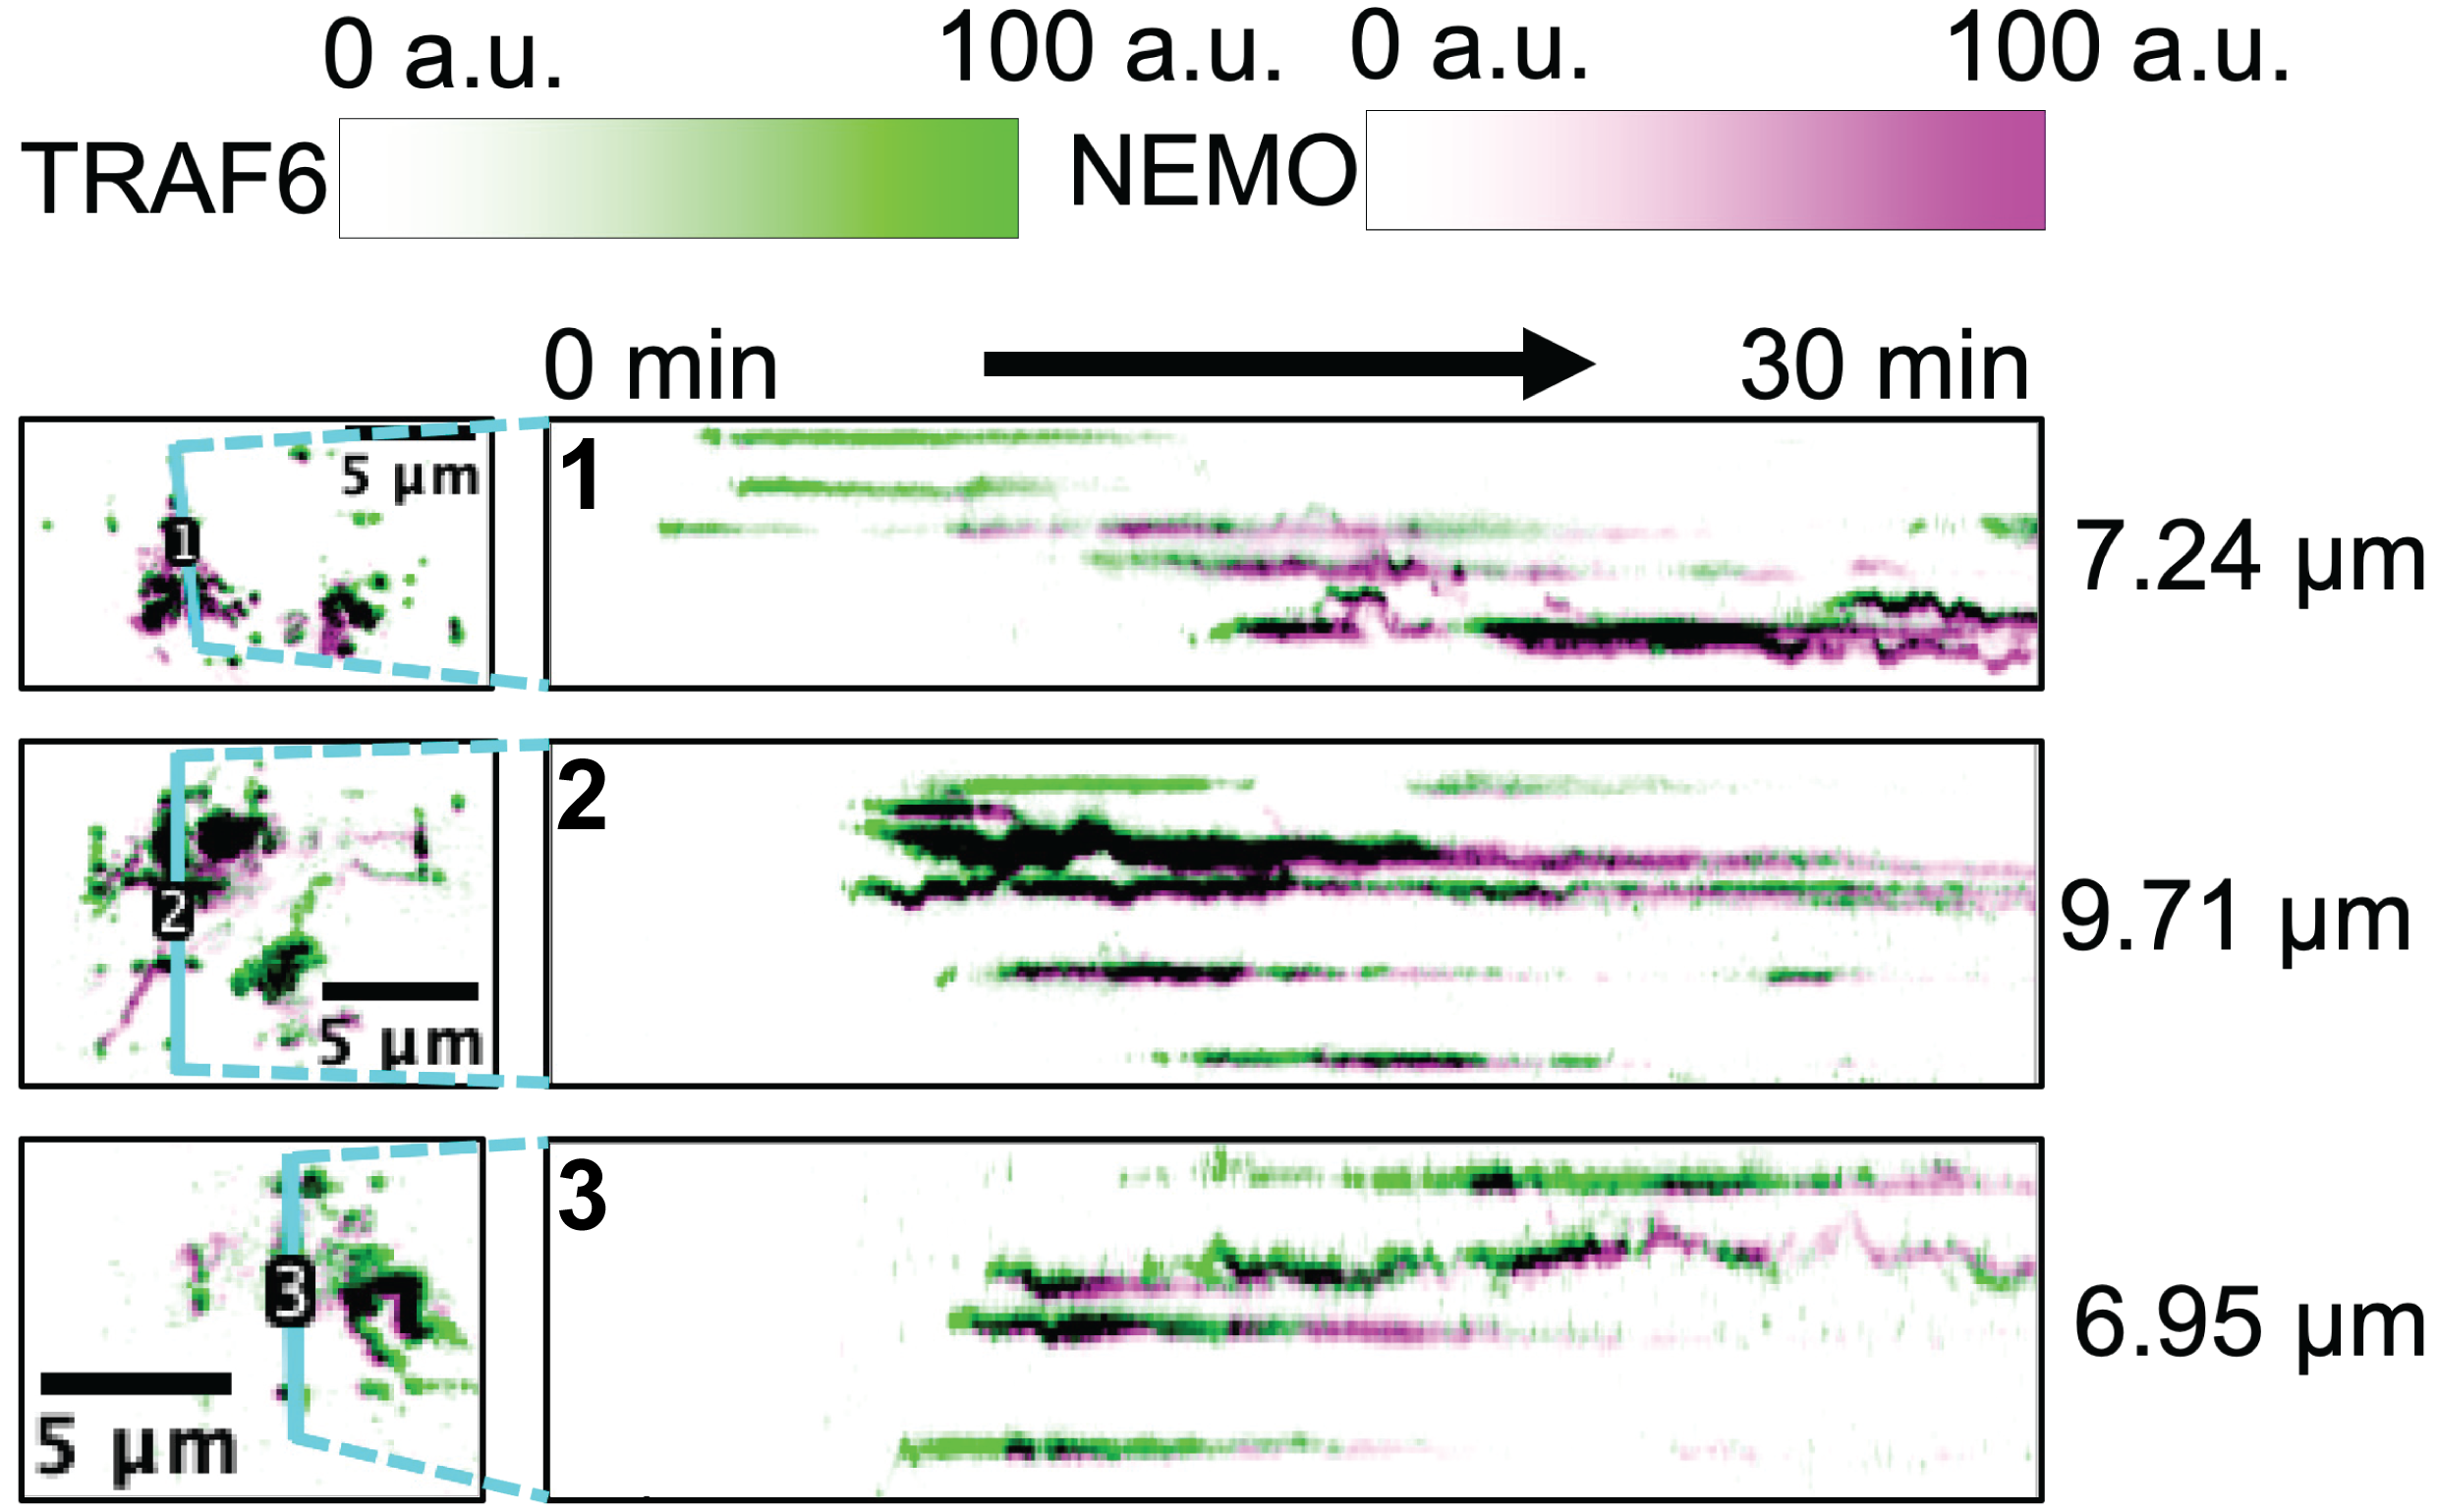
\includegraphics[width=\textwidth, height=\textheight, keepaspectratio]{mod/fig6a.png}}
\captionsetup{parbox=none}
\captionof{figure}[The IL-1 pathway disassembles the Myddosome signalosome first and then the NF-κB signalosome]{\textbf{The IL-1 pathway disassembles the Myddosome signalosome first and then the NF-κB signalosome.} Three kymographs of different lengths (y-axis) showing TRAF6 (green), NEMO (magenta), and merge (black) over time (x-axis). TRAF6 grows first (green), then NEMO colocalizes with TRAF6 (black), and TRAF6 leaves which leaves only NEMO (magenta), before NEMO disassembles (white). Each kymograph has a different scaling to fit the panel. (Imaging data courtesy of Elke Ziska.)}
\label{p2:6a}
\end{centering}

The cellular assembly dynamics of NEMO puncta has been documented \autocite{Tarantino_2014}\autocite{Du_2022}, but not with its interplay with Myddosome signalosome proteins. I plotted phase portraits for the TRAF6-NEMO images (Fig.~\ref{p2:3b}A). Here, I reveal a process where TRAF6 first expands, then recruits NEMO, followed by a sequential disassembly, starting with TRAF6 disassembling and finally, NEMO disassembly (Fig.~\ref{p2:6b}B).

Every diagonal line through the origin represents a constant stoichiometric ratio of equal proportions of TRAF6 to NEMO. The phase portraits showed orbital trajectories that were symmetrical upon the diagonal line (Fig.~\ref{p2:6b}A). This suggests that there is a critical stoichiometric ratio. Assemblies above the critical diagonal line are shrinking; and below, they are growing.

Taken together, the TRAF6-NEMO findings underscore the regulated nature of the IL-1 pathway, with stoichiometric ratios dictating the assembly and disassembly of proteins. Next, I will explore the shape of the phase portrait and its implications for protein assembly.


\begin{centering}
\centering{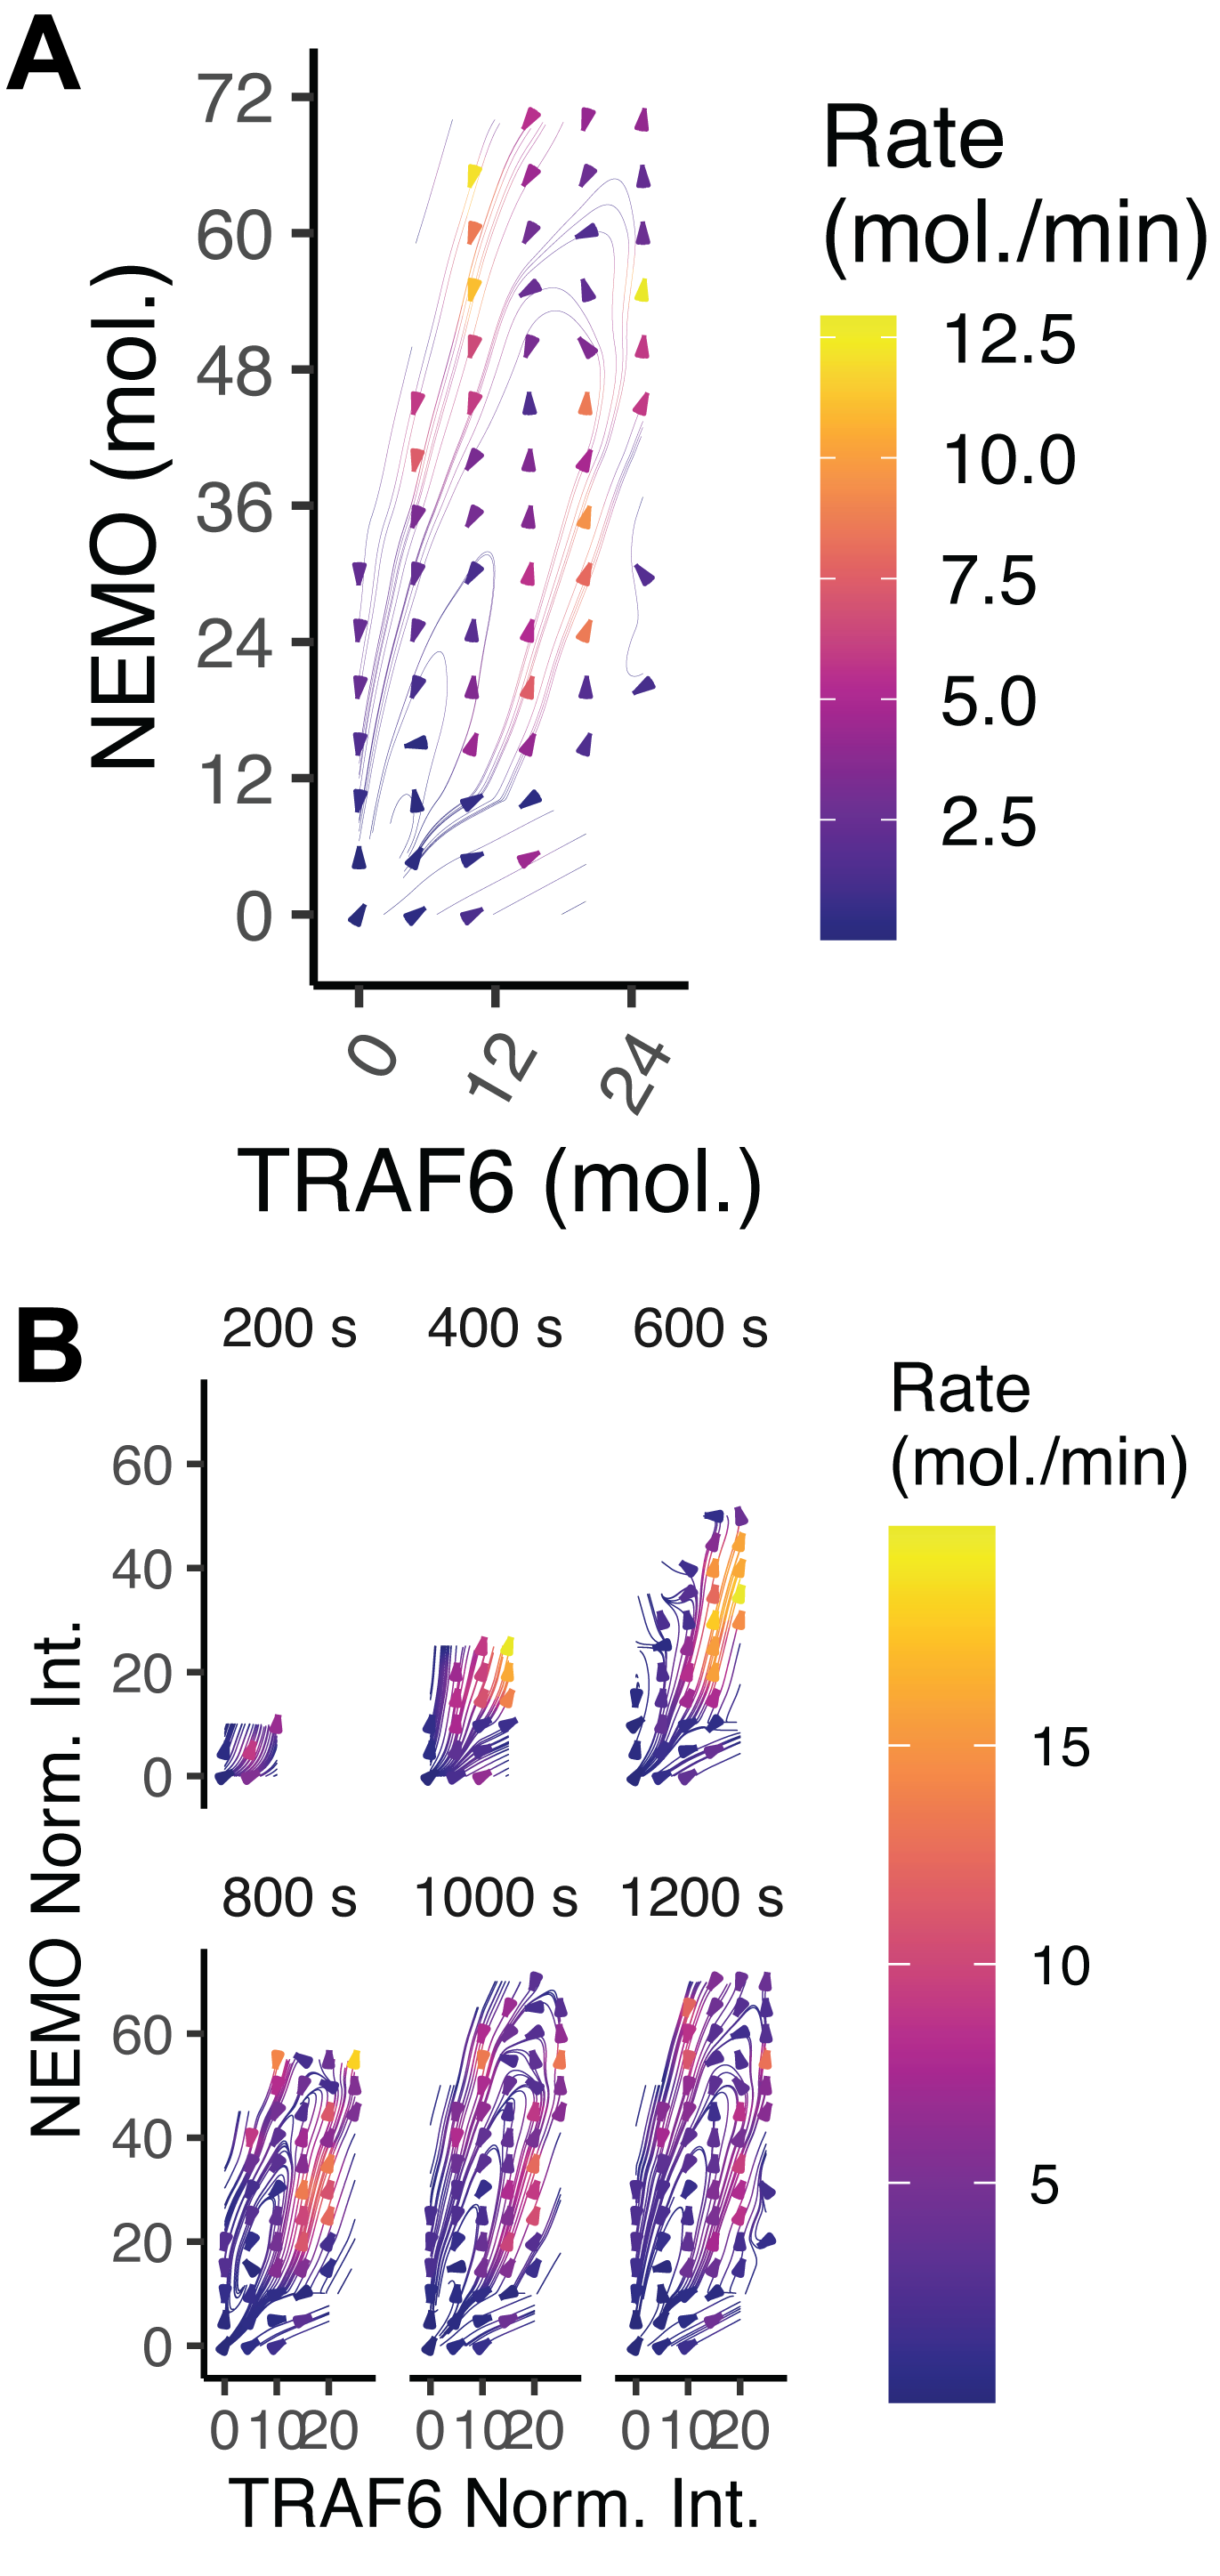
\includegraphics[height=0.75\textheight, keepaspectratio]{mod/fig6b.png}}
\captionsetup{parbox=none}
\captionof{figure}[IL-1 pathway shows orbital trajectories symmetric upon the diagonal line]{\textbf{IL-1 pathway shows orbital trajectories symmetric upon the diagonal line.}
\\
\\
(A) Phase portrait of TRAF6-NEMO. Streamlines are calculated independently using the arrow information provided to the phase portrait plot. Streamlines use the angle and magnitude of the phase portrait arrows, and are fitted using a forward Euler method for simple integration. This then plots an estimate of the solution of the differential equation. The mirror symmetry at the diagonal line indicates that the TRAF6 and NEMO sizes are proportional. The elliptical shape indicates more NEMO than TRAF6 in the puncta. The symmetry upon the diagonal suggests that the governing differential equations of this system are likely fractal-like (invariant to transformations). All diagonal lines represent a stoichiometric ratio. In this system, there is a diagonal line where puncta exhibit switch-like behavior, transitioning from assembly to disassembly. This “critical” diagonal line implies an unstable critical stoichiometric ratio. Crossing this diagonal line results in catastrophic disassembly. The orbital nature highlights the complex nature of this system due to non-linearity. Once a punctum follows a trajectory, it continues in the orbit. This sensitive dependence on initial conditions suggests a history-dependent system.
\\
\\
(B) Different time cutoffs based on the first puncta appearance. TRAF6 grows (200 seconds post first punctum), then NEMO grows together with TRAF6 (400 seconds), NEMO grows (600 seconds), TRAF6 disassembles , TRAF6 and NEMO disassemble and lastly, NEMO disassembles (800 seconds). The orbit returns to the origin, showing complete disassembly (0\times TRAF6, 0\times NEMO). The complete disassembly of the puncta indicates that the IL-1 signaling concludes with catastrophic disassembly. Once disassembly begins, TRAF6 and NEMO growth rates cannot keep up with the depolymerization rates. 
\\
\\
(A-B, I: Imaging data courtesy of Elke Ziska. Analysis, plots by the thesis author.)}
\label{p2:6b}
\end{centering}

\section{Dynamical equations that capture the feedback between IL-1 pathway modules}
\sectionmark{Predator-prey model}
\label{section:recapitulate_model}
\sectionmark{Predator-prey model}
It is remarkable that despite the large variability amongst individual IL-1 pathway protein structures (i.e., condensates, puncta), and the small number of molecules in each, the phase portraits (Fig.~\ref{p2:6b}) are able to show well defined average trajectories. As an aid to intuition, I note that these trajectories can be captured by a simple set of coupled dynamical equations. This set of equations constitutes a rough model that captures the major qualitative features of the phase portrait, and whose structure reflects the feedback motifs we have been discussing. With the TRAF6-NEMO images, we have directly observed the entire lifecycle of the IL-1 pathway. However, key questions remain unanswered: what triggers disassembly, and is there a theoretical model that accurately represents the experimental data? I aimed to develop a theoretical model that may encapsulate the observed experimental data. More specifically, my theoretical model makes use of differential equations. Differential equations are mathematical equations where the function is the derivative (rate of change).\footnote{Differential equations and phase portraits are explained in depth on the textbook \emph{Nonlinear dynamics and chaos} by Steven Strogatz \autocite{Strogatz_2018}} Differential equations have been extensively used in biology because they can help make predictions and test hypotheses, like done here. 

The simplest dynamical equations that capture the data are given in Fig.~\ref{p2:7}A. In the case of Fig.~\ref{p2:7}B, TRAF6 intensity is a proxy for the size of the Myddosome signalosome module and the NEMO intensity is a proxy for the size of the NF-κB signalosome module. The equations then represent the growth and feedback between these modules. I note that just growth ($\alpha x$, first term of equation 1), shrinkage ($-\gamma y$, last term of equation 2) and feedback ($-\beta xy$ and $\delta xy$, the cross terms) do not fully fit the data, suggesting that additional nonlinearities and potentially additional regulatory factors are involved. For the sake of the fit, in Fig.~\ref{p2:7}C, these nonlinearities are included as a term ($-\epsilon y^2$). However, the interpretation of such nonlinearities is beyond the scope of this thesis.


\begin{centering}
\centering{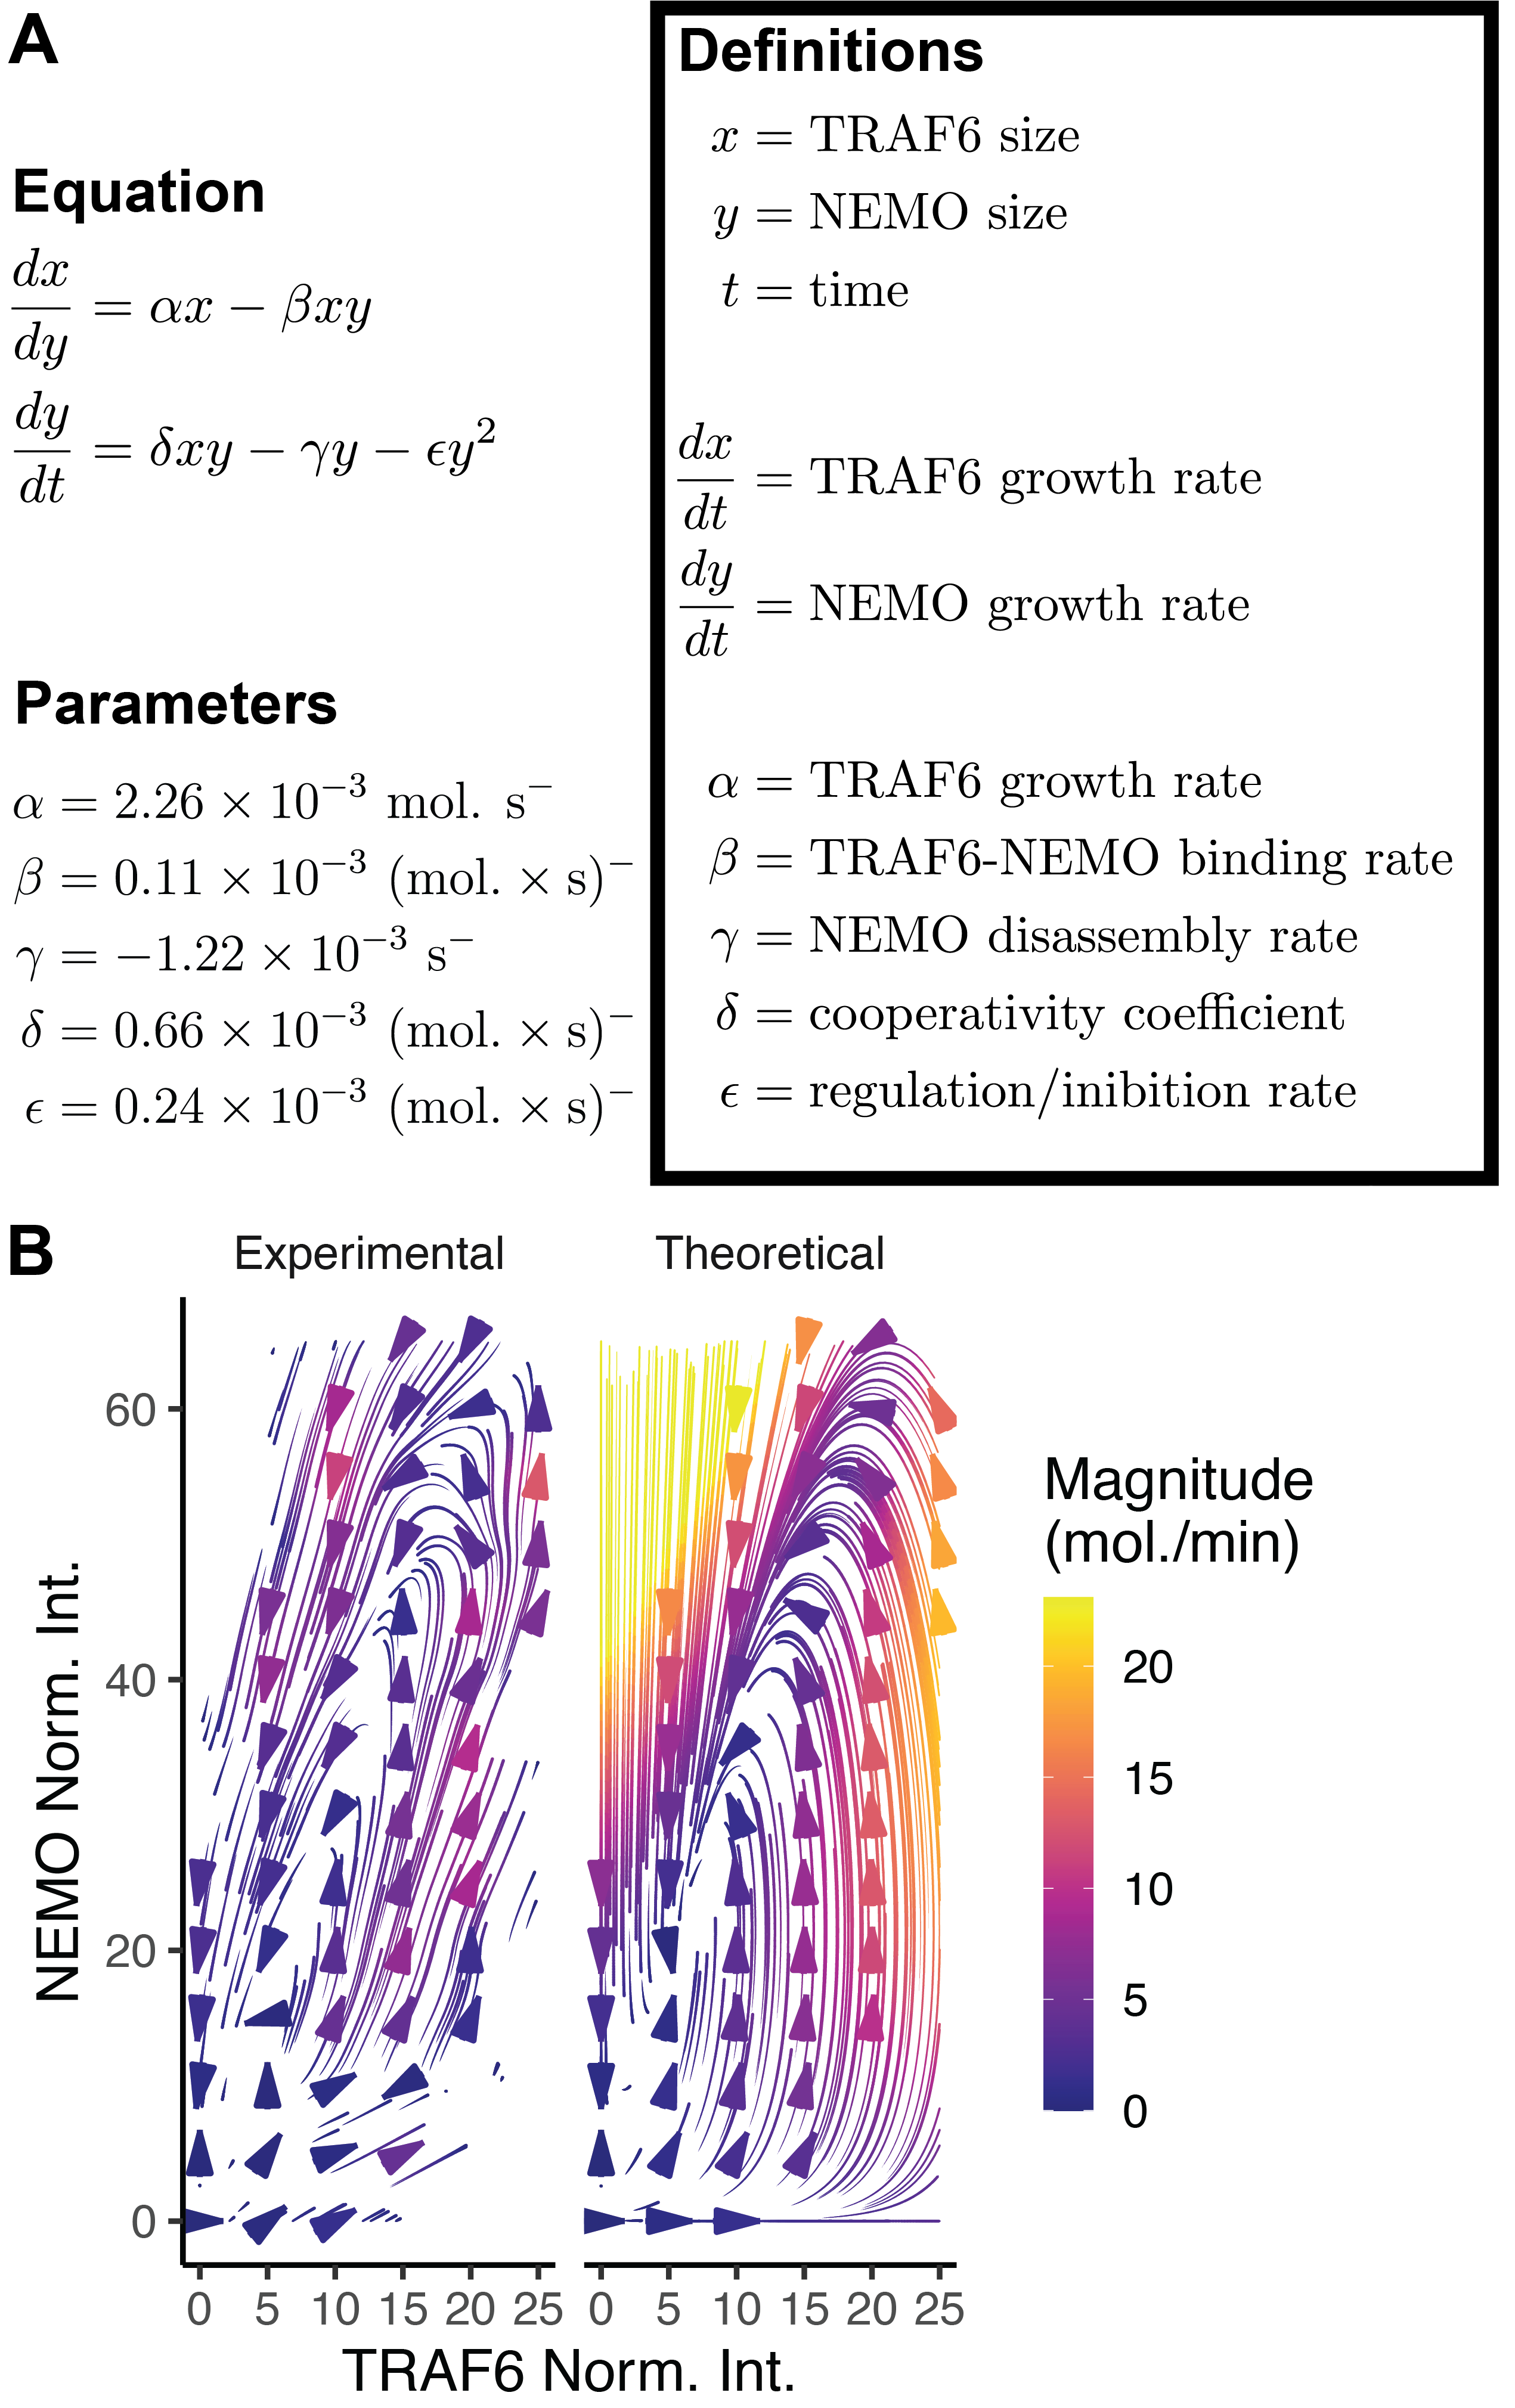
\includegraphics[width=\textwidth, height=\textheight, keepaspectratio]{mod/fig7.png}}
\captionsetup{parbox=none}
\captionof{figure}[The IL-1 pathway assembly and disassembly dynamics resemble predator-prey models]{\textbf{The IL-1 pathway assembly and disassembly dynamics resemble predator-prey models.}
\\
\\
(A) The experimental TRAF6-NEMO phase portrait displayed visual similarities to Lotka-Volterra equation phase portraits. However, while Lotka-Volterra phase portraits exhibit a “D” shape, the experimental phase portrait showed elliptical orbits. To accommodate this difference, a quadratic term, $-\epsilon y^2$, was introduced. The modified equation, parameters, and definitions are presented.
\\
\\
(B) A comparison of phase portraits for experimental data and theoretical predictions (R = 0.84) reveals a stable spiral. The theoretical model identifies a critical stoichiometry and predicts an unstable saddle point at 1.8\times TRAF6 and 22\times NEMO.
\\
\\
(B: Imaging data courtesy of Elke Ziska. Analysis, plots by the thesis author.)}
\label{p2:7}
\end{centering}


\begin{centering}
\centering{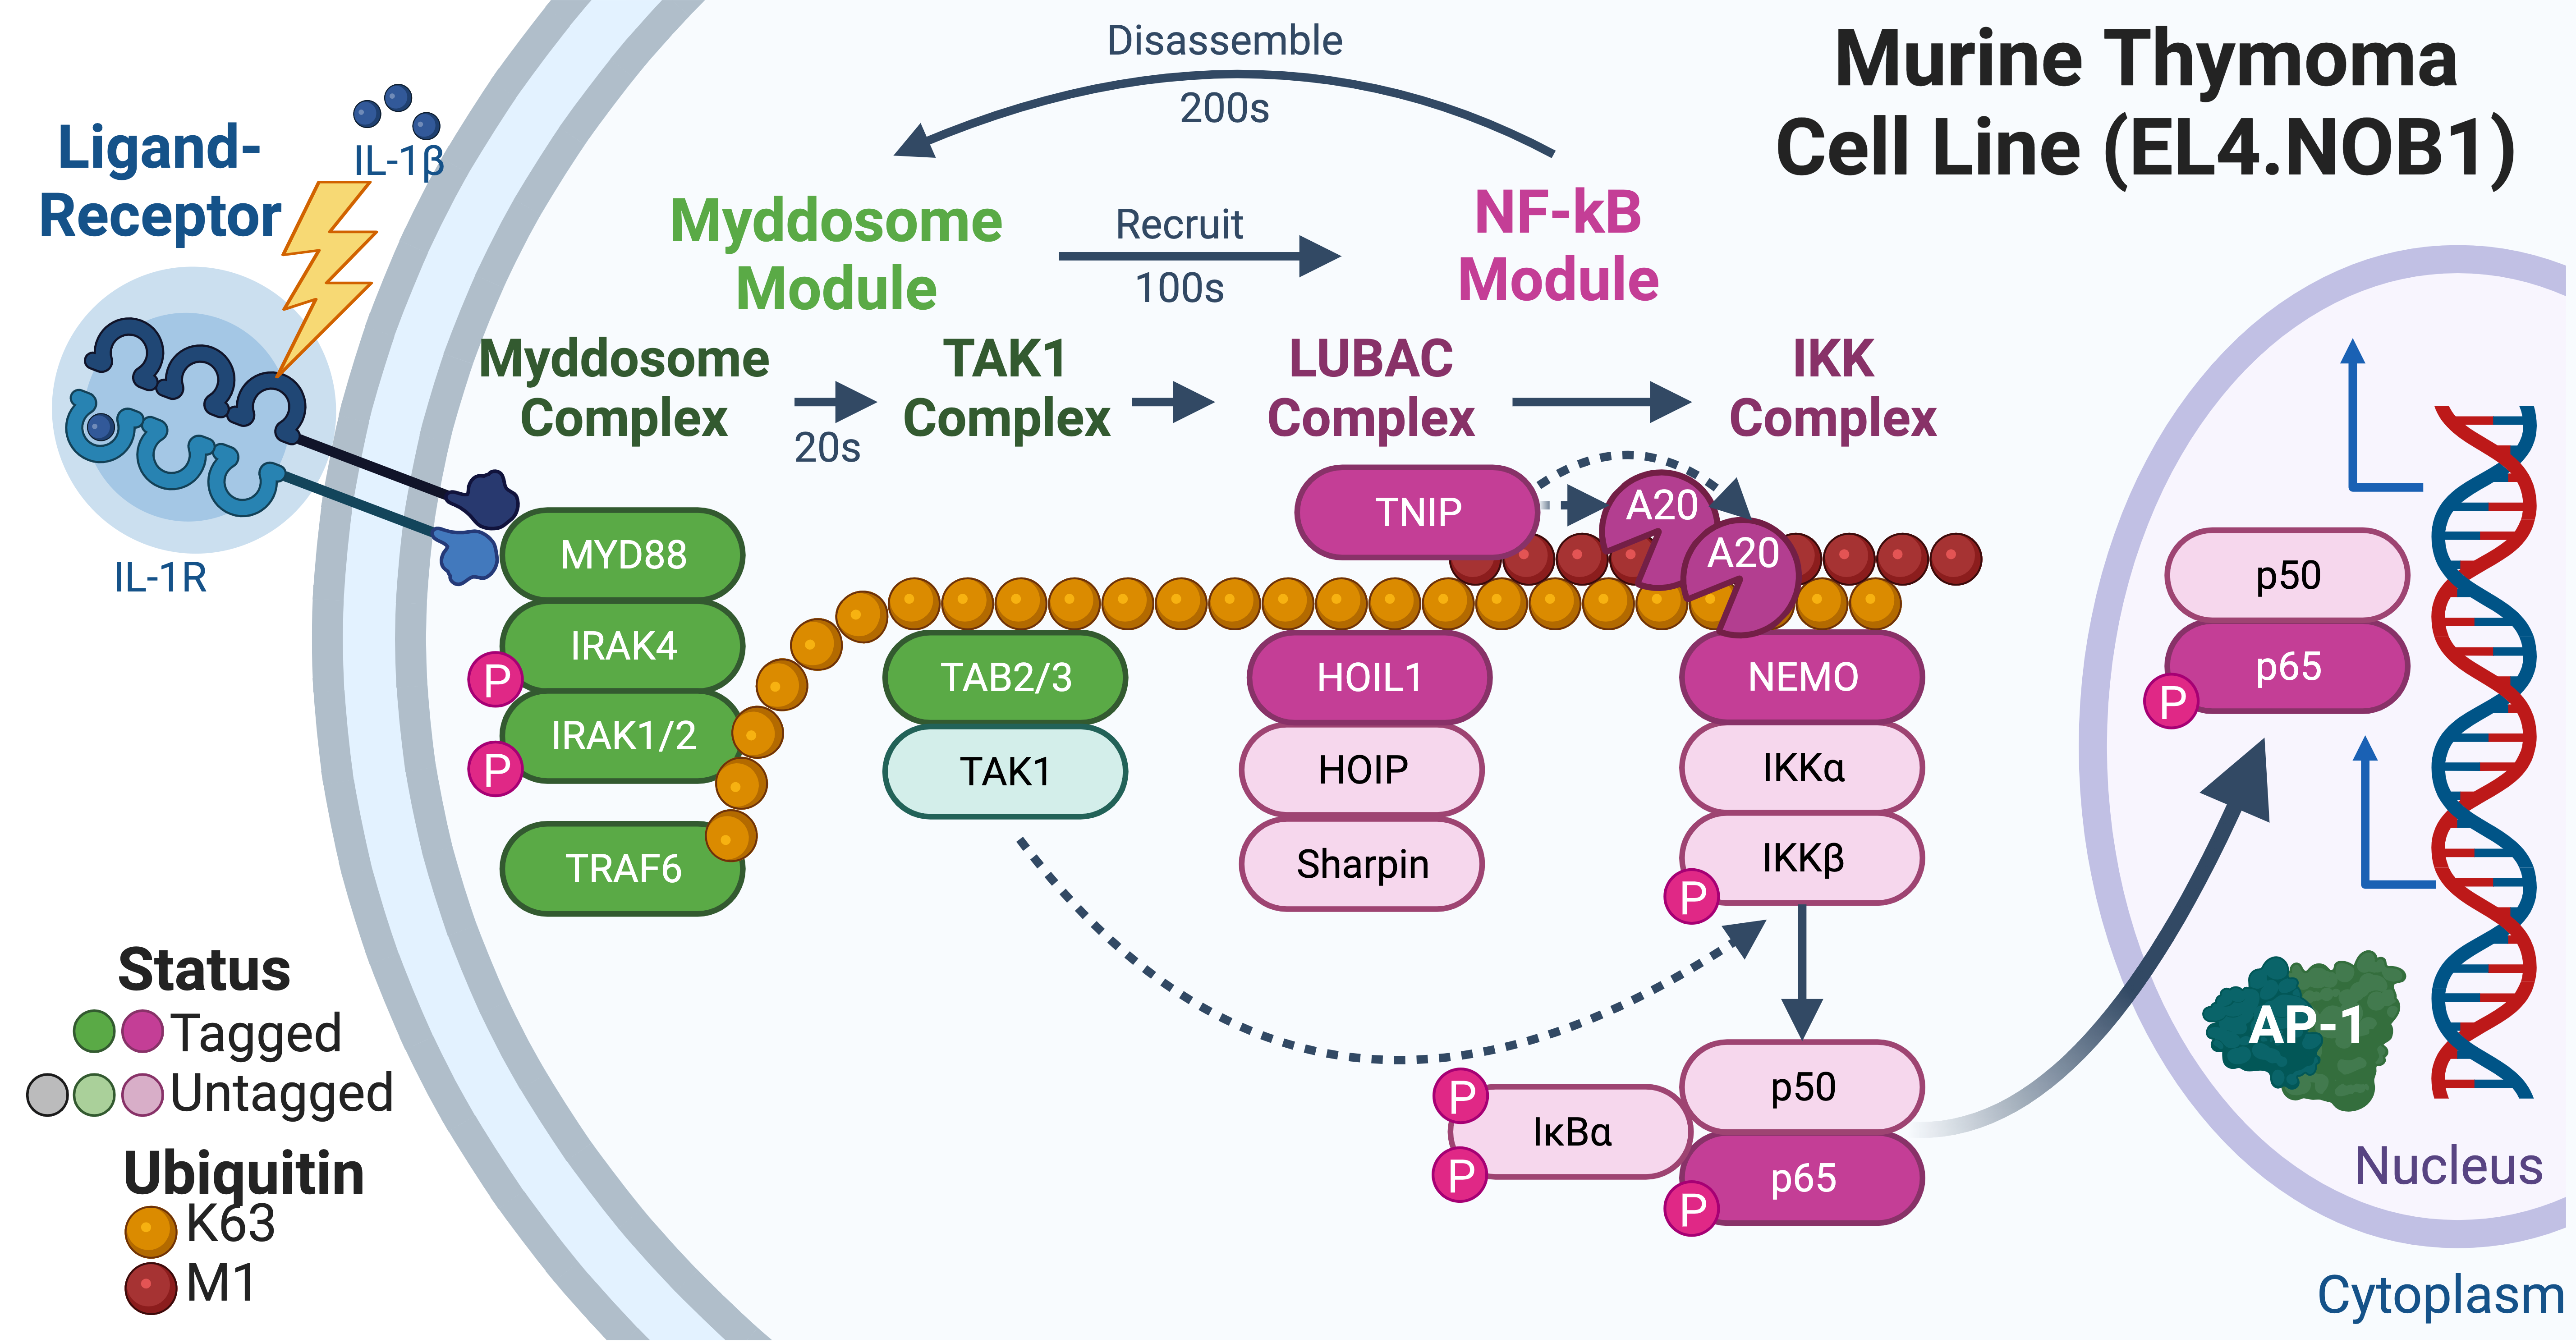
\includegraphics[width=\textwidth, height=\textheight, keepaspectratio]{mod/fig8.png}}
\captionsetup{parbox=none}
\captionof{figure}[A revisited model for the IL-1 pathway assembly and disassembly]{\textbf{A revisited model for the IL-1 pathway assembly and disassembly.} Based on this data, I propose the following model for IL-1 assembly: After IL-1 stimulates the IL-1R, the Myddosome assembles. Subsequently, TRAF6 and the TAB/TAK1 complex assemble, followed by LUBAC, the IKK complex, NF-κB, and finally, A20. The Myddosome signalosome disassembles, and lastly, the NF-κB signalosome disassembles.}
\label{p2:8}
\end{centering}

Three distinct methods have revealed two modules in the IL-1 pathway. They agreed on the proteins in each module, and showed distinct features of these modules, including their existence (Fig.~\ref{p2:1a}-~\ref{p2:1b}), their physical properties (Fig.~\ref{p2:2}), and their feedback (Fig.~\ref{p2:3},~\ref{p2:6b}-~\ref{p2:7}).

In conclusion, the modular nature of the IL-1 pathway, the distinct roles of the Myddosome and NF-κB signalosomes in signal transduction, and the utility of modified Lotka-Volterra equations in modeling protein assembly and disassembly dynamics constitute significant findings from this study. These results enhance our mechanistic understanding of the oligomerization of the IL-1 pathway, with potential implications for other Supramolecular Organizing Centers that similarly leverage oligomerization. Thus, this study may open a new paradigm in signal transduction, pending future experimentation.

\mygeometry
\part{Discussion}
\restoregeometry
\chapter{Discussion}
\section{Myddosome assembly and disassembly dynamics may apply to other SMOCs}
\sectionmark{Myddosomes and SMOCs}
I have shown how the proinflammatory IL-1 pathway transduces its signal through nine key proteins. By building a new image analysis pipeline, this work unraveled the intricate mechanisms of assembly and disassembly of the IL-1 pathway proteins, positioning it as a kinetic model for several innate immune signaling pathways called supramolecular organizing complexes, or SMOCs for short \autocite{Kagan_2014}.\footnote{More on SMOCs at Introduction~\ref{section:SMOC}}

SMOCs are higher-order punctate structures that employ oligomerization for signal transduction \autocite{Kagan_2014}. Each SMOC possesses both an input ligand and an output mediator, and is characterized by their helical filament structure. Example SMOCs are FAS DISC, PIDDosome, Myddosome, RLR complex, and the inflammasome \autocite{Kagan_2014}. Our understanding of SMOCs has largely been based on structural and biochemical approaches \autocite{Balka_2019}\autocite{Kagan_2014}. However, these approaches often leave the dynamics of SMOCs underexplored, largely missing because of the limitations of said structural and biochemical methods.

Compared to previous studies \autocite{Latty_2018}\autocite{Moncrieffe_2020}, my new angle offers improved spatial and temporal resolution of SMOC dynamics. My new approach found modularity and perhaps predator-prey interactions in the relationships between IL-1 pathway proteins,\footnote{Predator-prey interactions discussed in Introduction~\ref{subsection:predator_prey}} offering a new paradigm for the assembly and disassembly mechanisms of SMOCs, pending further testing. Given that the Myddosome is a member of the SMOC family, characteristics observed in the Myddosome, such as its disassembly, might also be relevant to other SMOCs.

My distinct interrogation of the IL-1 pathway provides a potential framework for the amplification of signals through oligomerization within SMOCs, and broadens our understanding of signaling pathways and their critical roles in orchestrating responses. These discoveries in immune responses could have a wider application in the fields of immunology, infection biology, cell biology, and synthetic biology where pathways are plentiful.

\section{IL-1 pathway oligomerize inducibly, sequentially}
\sectionmark{Inducible & sequential}
This study demonstrates the \emph{de novo} assembly of the Myddosome complex, aligning with the hypothesis proposed by \autocite{Lin_2010}. This is supported by the observed growth of MyD88 assemblies over time (Fig. ~\ref{p1:3c}B,~\ref{p2:1b}B), potentially dismissing the preformed scaffold hypothesis supported by analytical ultracentrifugation and cryoEM \autocite{Motshwene_2009}\autocite{Moncrieffe_2020}.

Prior investigation suggested that Myddosome assembly occurs in a sequential manner \autocite{Lin_2010}\autocite{Moncrieffe_2020}. This work showed that the mid-assembly timepoint is able to reproduce sequences comparable to recruitment times. The IL-1 pathway begins with the nucleation of MyD88, followed by IRAK4 recruitment 14 seconds later, and IRAK1 recruitment 27 seconds later (Fig.~\ref{p1:4c}B). The ensuing assembly sequence observed in the IL-1 pathway is TRAF6, TAB2, RelA, NEMO and finally, A20 (Fig.~\ref{p2:1b}B).

HOIL1 reached mid-assembly earlier (Fig.~\ref{p2:1b}B) than expected \autocite{Cohen_2020}. HOIL1 is a ligase that forms M1-ubiquitin chains \autocite{Kelsall_2019}. It is known that MyD88 forms M1-ubiquitin chains quickly \autocite{Cohen_2020}\autocite{Cohen_2017}. Therefore, the microscopy in this study has shown that HOIL1 interacts with the Myddosome. This supports a previously reported immunoprecipitation experiment where the Myddosome and HOIL1 were shown to interact via K63-ubiquitin chains \autocite{Kelsall_2019}.

The IL-1 pathway proteins assembly sequence (Fig.~\ref{p2:1b}) shows RelA reaching mid-assembly before NEMO. This could be that NEMO continues to coalesce even after RelA activation. Trimers of RelA were also observed in the absence of MyD88, suggesting faster mid-assembly due to the presence of RelA multimers in the cytosol (Fig.~\ref{p2:S1}D).

However, the mid-assembly timepoint approach could have limitations, such as the difficulty in identifying simultaneous assembly of multiple protein types. For example, IRAK1 and HOIL1 could have simultaneous binding to different binding sites, and thus, their mid-assembly times are indistinguishable. This could potentially be overcomed by introducing ligand titration in future experiments because downstream protein recruitment depends on stable complexes, and more stable complexes can be formed with higher ligand densities. Inversely, lower ligand density would highlight which protein assembles preferentially.

Nevertheless, the assembly sequence of the IL-1 pathway is important because it helps establish the relationship among proteins. This allows targeting at the height of activity. Moreover, the mid-assembly timepoint informs when a complex reaches an assembled state, something that the recruitment time cannot capture because of its bias to earlier timepoints due to protein sampling.

In summary, the findings of this study indicate that the IL-1 pathway protein assembly is through ligand-induced \emph{de novo} oligomerization and sequential, and not pre-assembled \autocite{Moncrieffe_2020}.

\section{IRAK4 regulates MyD88 oligomer size}
While the IRAK4 kinase activity was found to be dispensable for Myddosome assembly, its structural role remained unclear \autocite{DeNardo_2018}. This observation suggests an autoregulatory mechanism in the IL-1 pathway, with IRAK4 functioning as a limiting factor (similar to capping) to MyD88 oligomerization. The specific role of IRAK4 in this autoregulation, and particularly whether the oligomer length of IRAK4 is regulated by the kinase activities of IRAK4 or IRAK1, remains unclear. To fully understand the autoregulatory mechanisms, further investigation is required in these areas.

Future research should also aim to determine if IRAK1 is capable of capping IRAK4 oligomerization, which would offer additional insights into the autoregulatory mechanisms of the IL-1 pathway.

These findings and proposed future directions contribute to our growing understanding of the complex regulatory mechanisms underpinning immune signaling pathways.

This study showed that without IRAK4, MyD88 oligomerizes until all cytosolic MyD88 is exhausted (Figs.~\ref{p1:6a}-~\ref{p1:6b}). 
\section{Two signalosomes in the IL-1 pathway}
In this study, I reveal previously unknown feedback mechanisms of the IL-1 pathway assembly using phase portrait to analyze colocalization (Fig.~\ref{p2:S1}A-D). This novel approach allowed the delineation of the pathway into two signalosomes based on distinct feedback mechanisms: the Myddosome and the NF-κB signalosomes. Specifically, the Myddosome signalosome proteins IRAK4, IRAK1, TRAF6, and TAB2 exhibited positive feedback relative to MyD88 (Fig.~\ref{p2:S2}A), while the NF-κB signalosome proteins HOIL1, NEMO, RelA, and A20 exhibited negative feedback relative to MyD88 and TRAF6 (Fig.~\ref{p2:S2}C).

Interestingly, all NF-κB signalosome components (HOIL1, NEMO, RelA, and A20) are shared with the TNF signaling pathway, with the addition of TRAF6 and TAB2. Perhaps TRAF6 is an adaptor protein to the NF-κB signalosome, and TAK1-TAB2 to a hypothetical MAPK signalosome. I speculate that like the IL-1β pathway, the TNFα pathway also has two signalosomes: (1) the TRADDosome signalosome, and (2) the NF-κB signalosome. Furthermore, perhaps the TRADDosome and RLR complex together form filaments, given that the RLR complex is a filament \autocite{Kagan_2014}, and TRADD has death domains \autocite{Michallet_2008}. More broadly, the trend may be that SMOC adaptors are filaments and that SMOC effectors recover after photobleaching, perhaps as phase-separated condensates.

These new findings (Fig.~\ref{p2:8}) reshape our understanding of the IL-1 pathway, which was previously viewed as a mesh network (Fig~\ref{img:interactome}) \autocite{Cohen_2020}\autocite{Zarrin_2021}\autocite{Zinatizadeh_2021}. Instead, I now characterized it as having at least two distinct signalosomes. Within each signalosome (intra-modularly), there is internal feedback consistency, but between the two (inter-modularly), the feedback juxtaposes.

These results not only provide a more detailed understanding of the IL-1 pathway assembly, but also suggest a higher-order level of modularity in TLR/IL-1 pathways to achieve regulation. Furthermore, the identification of these higher-order modules offer a broader perspective on immune response regulation where they may be more prevalent as regulatory modules, and could explain similar responses to diverse inputs.

Providing a regulated modules model of the IL-1 pathway as an example, this study invites microscope users across disciplines to consider using phase portraits to analyze colocalization and identify modules and regulation. Understanding the modularity of signaling pathways could potentially pave the way to identifying new signalosomes, and open new intervention strategies for therapeutics.

\section{The IL-1 pathway disassembles}
The disassembly of the IL-1 pathway is a critical aspect of its function, but it remained largely unclear \autocite{Balka_2019}. The second aim of this study was to identify whether the IL-1 pathway undergoes disassembly. To investigate the disassembly process, Elke Ziska generated and imaged the TRAF6-NEMO cell line, and then I applied phase portrait analysis.

I found that TRAF6-NEMO puncta exhibit a disassembly phase (Fig.~\ref{p2:3}A), with TRAF6 disassembly triggered in the presence of large NEMO assemblies (Fig.~\ref{p2:S2}C). This finding contributes to our mechanistic understanding of IL-1 pathway disassembly, suggesting a possible predator-prey relationship between TRAF6 and NEMO, with a 35\% TRAF6:NEMO critical stoichiometric ratio dictating the disassembly process.

However, uncertainty remains as several modes have been proposed to describe the disassembly mechanism of the Myddosome, such as the internalization of Myddosomes via lipid rafts \autocite{Triantafilou_2004}\autocite{Triantafilou_2006}\autocite{Barbalat_2009}\autocite{Ruysschaert_2015}, Myddosomes detaching from the receptor \autocite{Latty_2018}, 

the formation of vesicles by activated Myddosomes,
\autocite{Balka_2019}\autocite{Thieblemont_1999}\autocite{Kagan_2008}\autocite{Manček-Keber_2018}\autocite{Nguyen_2017}. The diminishing puncta intensities observed could be explained by some of these disassembly models, though they do not explain how the signal intensity decreases for the Myddosome, the structure closest to the receptor, before the NF-κB signalosome. One explanation could be that TRAF6 bleached because it appeared first. Yet the fluorophore lifetime is longer than the disassembly timepoint, hence the assumption that disassembly was observed.

Overall, this study not only provides new insights into the IL-1 pathway disassembly dynamics but also highlights the potential of using predator-prey models as a means to understand signaling protein dynamics. Future research would benefit from further investigating protein interactions in the IL-1 pathway and SMOCs using predator-prey models to unveil the underlying mechanisms governing their assembly and disassembly dynamics.

\section{Cytoskeleton dynamics may inform Myddosome dynamics}
\sectionmark{Cytoskeleton dynamics}
\label{section:cytoskeleton}
\sectionmark{Cytoskeleton dynamics}
The Myddosome is a complex helical filament composed of death domains \autocite{Moncrieffe_2020} that possesses structural and dynamic properties similar to the cellular cytoskeleton component actin. The dynamic assembly and disassembly of actin, well-documented in the literature, provides a potentially insightful framework for probing the hitherto enigmatic dynamics of the Myddosome assembly and disassembly.
 
The assembly mechanism of the Myddosome remained a subject veiled in mystery.\footnote{Myddosome assembly discussed in Introduction~\ref{subsection:assembly}} However, the Myddosome is understood to use polymerization \autocite{Lin_2010}, a strategy also employed by the cytoskeleton \autocite{Mogilner_1996}. Like actin, which assembles from globular and filamentous monomers \autocite{Cooper_2000}, the Myddosome comprises an assortment of proteins: MyD88, IRAK4 and IRAK1/2 \autocite{Lin_2010}. In an intriguing parallel, we discovered that the Myddosome, like actin, demonstrates ligand-induced oligomerization \autocite{Deliz-Aguirre_2021}. This underscores the striking similarities between the Myddosome and actin assembly mechanisms.
 
When it comes to the Myddosome disassembly, it is largely uncharted territory.\footnote{Myddosome disassembly discussed in Introduction~\ref{subsection:disassembly}} Yet, I postulate that it mirrors patterns observed in other oligomeric filaments, such as the dynamic instability that precipitates the cytoskeleton’s structural collapse \autocite{Mitchison_1984}. The initial findings suggested that the Myddosome exhibits an instability akin to actin, particularly pronounced in shorter oligomers \autocite{Deliz-Aguirre_2021}. Similar to the dynamic instability of actin \autocite{Kueh_2009}, the dynamic instability model of the Myddosome I propose entails that interactions are weak, transient and highly susceptible to changes in the activation states of the interactors. This model offers a plausible explanation to how phosphorylation states of the IRAKs influence the binding affinity of Myddosome components \autocite{DeNardo_2018}. Recent research also highlighted the role of dynamic instability in mediating the actomyosin cortex activation of \emph{Caenorhabditis elegans} \autocite{Yan_2022}. They found that condensates grow, but then disassemble before dissolving completely \autocite{Yan_2022}. Their findings provide a valuable context for studying the Myddosome dynamics through the lens of cytoskeleton dynamics.
 
Actin filament dynamics are regulated by other proteins \autocite{Lee_2010}\autocite{Kashina_2020}. Similarly, the Myddosome assembly and disassembly dynamics, largely uncharted until now, may be influenced by other downstream IL-1 signaling proteins. Corroborating this possibility, we found that within the Myddosome, IRAK4 influences the length of MyD88 oligomers \autocite{Deliz-Aguirre_2021}. This thesis will provide an in-depth exploration of these other IL-1 pathway proteins using live cell imaging.

The disassembly of the TRAF6-NEMO assembly is reminiscent of cytoskeleton dynamics, where actin filaments catastrophically collapse.

\section{The new image analysis pipeline quantified images at an unprecedented scale}
\sectionmark{High-throughput pipeline}
Understanding the cellular machinery requires accurate quantification. Image analysis has emerged as a vital tool to address this in cell biology. We are now able to unravel stoichiometries and pathway dynamics using microscopy. However, efficient processing of large volumes of microscope images for molecular analysis remains a key challenge.

In this study, I present the PIRATES-PARLEYS (Pipeline for Image analysis with Reference images, Automated Tracking, Extraction of intensities, and Segmentation “PIRATES” Phase portrait Analysis and Relative kinetics comparison Localization analysis with Extraction of data Yielding Statistics “PARLEYS”), an image analysis pipeline that addresses this issue. Here, I show that this dual wet-dry bench pipeline is capable of not only converting images into meaningful stoichiometries but also rapidly analyzing a large volume of images. As revealed by phase portrait analysis, the pipeline was able to resolve molecular details down to monomers (Fig.~\ref{p2:3},~\ref{p2:S5}). This adds to the repertoire of image processing techniques by enabling analysis with unprecedented detail and speed. The improved resolution is owed to the large sample size, and the consolidation of image processing strategies (see Methods~\ref{chapter:PIRATES_PARLEYS}).

The results redefine our expectations from image analysis in molecular biology, breaking new ground in the study of protein dynamics and opening up avenues for broader applications. In a broader context, this image analysis pipeline could be extended to the puncta of proteins in the IL-1 pathway and other biological pathways, thus paving the way for future breakthroughs in cellular and molecular biology.

\chapter{Limitations}
\section{Observations are confined to diffraction-limited puncta dynamics}
\sectionmark{Diffraction-limited}
The ability of light microscopy to discern minute structures is intrinsically constrained by Abbe’s principle, stating the diffraction limit of spatial resolution cannot resolve structures smaller than half the wavelength of light \autocite{Heintzmann_2006}. Consequently, the findings from this study, predominantly reliant on Total Internal Reflection Fluorescence (TIRF) microscopy, are restricted to diffraction-limited puncta \autocite{Ruckstuhl_2003}.

Each Myddosome, a key structural module in this study, measures approximately 10-1000 nm long and 6.8 nm in diameter \autocite{Moncrieffe_2020}. Given the emission wavelengths of the fluorescent proteins employed, eGFP (507 nm) and mScarlet (594 nm), and applying Abbe's principle, we find the spatial resolution in the xy-plane is 199 nm.
\begin{equation*}
\begin{aligned}
\text{resolution}_\text{xy} &= \frac{\lambda}{2\text{ NA}} \\
&= \frac{594 \text{ nm}}{2 \times 1.49} \\
&= 199 \text{ nm}
\end{aligned}
\end{equation*}
With a camera resolution of 146 nm and puncta diameter of 730 nm, at least 20, and potentially up to 107 Myddosomes could theoretically fit within a single puncta. Thus, the observed dynamics potentially encompass more than one Myddosome assembly, leading to an underrepresentation of the full complexity of the IL-1 pathway.

Several strategies were employed to mitigate this limitation. Notably, one ligand density was chosen to allow observing dynamic events on the timescale of minutes, while minimizing the risk of Myddosome coalescence into larger super-Myddosome assemblies. Future work may use chromium grids to form cellular corrals \autocite{Huang_2019} , thereby limiting Myddosome coalescence \autocite{Cao_2023}.

Furthermore, comparing experimentally derived stoichiometries with those reported in the literature \autocite{Lin_2010}\autocite{Moncrieffe_2020}\autocite{Ye_2002} offers indications of single Myddosome observations. However, challenges in determining the precise structure of Myddosomes due to their variable length and small size (Fig.~\ref{p2:S1}, \autocite{Moncrieffe_2020} calls for alternative methodologies. Super-resolution microscopy techniques such as STORM, PALM, or SIM \autocite{Huang_2010}, along with computational tools such as AlphaFold \autocite{Nussinov_2022}, could help decipher sub-diffraction structures to better understand Myddosome and the IL-1 pathway architecture in future studies.

In summary, while the observations made in this study provide valuable insights into the IL-1 pathway dynamics, they must be considered within the inherent limitations posed by diffraction-limited microscopy. The complexity of the IL-1 pathway may extend beyond what is currently observable and future research employing more advanced imaging modalities will be pivotal to unraveling these intricacies.

\section{Current fluorophores are limited in spatiotemporal resolution}
\sectionmark{Fluorophore limits}
The 3D architecture of the Myddosome and NF-κB signalosomes remains elusive. Details inside diffraction-limited puncta could be resolved using superresolution microscopy. Theoretically, this could ascertain the filamentous nature of Myddosomes \autocite{Moncrieffe_2020}, and in particular, the Myddosome signalosome. However, the IL-1 pathway proteins present several challenges for superresolution microscopy.

Myddosomes are small relative to other SMOCs \autocite{Kagan_2014}\autocite{Lin_2010}. This means that there is a low fluorophore count when tagging Myddosome proteins. Superresolution microscopy uses an increased light power to achieve a higher spatial resolution. Imaging the fluorescent tags used in this study (eGFP, mScarlet) would result in some bleaching before details emerge. This translates to loss of signal and inaccurate quantification \autocite{Thorley_2014}.

A solution could be to switch the fluorophore for more stable ones (for example, organic dyes) \autocite{Grimm_2017}. However, selecting fluorophores presents its own set of challenges. Several factors need to be accounted for, including solubility, molecular weight, spectral properties (for example, to avoid overlap, for matching equipment), maturation times, photostability, and biological compatibility to avoid steric hindrance, function impairment \autocite{Verkhusha_2004}\autocite{Zheng_2014}. AlphaFold and similar technologies could help the user in offering a preliminary selection of the best fluorophores, but ultimately, it requires validation at the wet lab. Moreover, generating CRISPR/Cas9 edited cell lines has its own set of challenges. As previously mentioned, crystallography and cryogenic electron microscopy also have their limitations.

Assessing the 3D architecture of the IL-1 pathway using current technology remains a technical challenge. The current toolkit has a limited ability to resolve the heterogeneous structures formed.

\section{Only one ligand density regimen was thoroughly tested}
\sectionmark{One ligand density}
The IL-1 pathway response is graded by ligand density \autocite{Latty_2018}\autocite{DeFelice_2019}. Controlling the ligand density with supported lipid bilayer (SLB) technology offers an opportunity to elucidate signaling dynamics. However, the question remains: how does ligand density affect the kinetics of IL-1 pathway assembly? In this study, I show the practicality of a single ligand density emulating physiological conditions to simplify and standardize the interrogation of IL-1 pathway assembly.

Departing from the prevailing titration in medium approach, I used SLB to yield a tightly-controlled single ligand density that offers reproducible results and insights into IL-1 pathway assembly dynamics. This approach, however, acknowledges the implicit oversimplification with the potential to overlook subtleties in the ligand dose-response. Nevertheless, it offers an advantage in reducing experimental variability and enabling on-prompt oligomerization.

A limitation of this study lies in the data acquisition rate. The wet bench imaging protocol, although highly reproducible, is time-intensive and constrained by equipment availability. The introduction of additional users to increase throughput may inadvertently introduce experimental variability. Future efforts might explore automating the imaging pipeline and integrating data modeling for efficiency, thus potentially allowing the exploration of how different ligand densities affect the phase portraits.

In the broader context, while the ligand density indeed represents a crucial variable in the IL-1 pathway, comprehensive study necessitates vast resources due to the requirement for large sample sizes. Yet, the approach illustrated here reveals the potential to gather meaningful insights through targeted stimulation near physiological conditions, offering a more manageable route for future research in this area.

\section{Not all proteins and their combinations were tested}
\sectionmark{Limited protein combinations}
In the realm of inflammatory responses, the IL-1 pathway stands central. Because of that, there is a long list of protein interactors. This study focused on comparing MyD88 with key downstream proteins and also, TRAF6 with NEMO. However, the imaging of all possible protein combinations and known pathway proteins remains incomplete. The adopted methodology, CRISPR/Cas9 for gene editing of cell lines, presents significant time limitations as it spans months.

Here, I reveal that a key set of protein interactions within the IL-1 pathway, specifically, MyD88-TRAF6, MyD88-NEMO, and TRAF6-NEMO, exhibit analogous dynamics. This implies that the IL-1 pathway assembly might be modular, suggesting that exhaustive testing of all protein combinations may not necessarily expand our understanding of the pathway significantly. Nonetheless, the process of generating new cell lines is a fundamental limitation, being resource and time-intensive.

Beyond the confines of this study, dynamics within the NF-κB signalosome and Fluorescence Recovery After Photobleaching (FRAP) data for TAB2, NEMO, RelA, and A20 were not addressed. These could form the cornerstone of future work, aimed at validating the modularity of the IL-1 pathway. The addition of more cell lines might also enhance the robustness of this validation, though with a cautionary note that a saturation point may exist beyond which further testing offers minimal additional insight.

Overall, our work lays the groundwork for a new perspective on IL-1 pathway assembly, highlighting the potential modularity of its components. The limitations delineated here, while constraining, also pave the way for targeted future investigations to consolidate and broaden our understanding of IL-1 signaling dynamics.

\chapter{Outlook}
\section{Could other innate immune pathways have similar dynamics to IL-1?}
\sectionmark{Applicable to other pathways}
Signal transduction mechanisms are fundamental to the orchestration of cellular responses to stimuli. A subset of these signaling pathways, known as Supramolecular Organizing Centers (SMOCs), play a pivotal role in the innate immune system, sharing similarities in their signaling mechanism \autocite{Kagan_2014}. The Myddosome, an established SMOC, forms inducible helical filaments \autocite{Moncrieffe_2020}. The filament trait is shared with other SMOCs, including MAVS CARD and ASC, through the process of oligomerization \autocite{Xu_2014}\autocite{Nambayan_2019}.

This study probes the question of whether there are commonalities in assembly mechanisms, size thresholding, regulatory controls, and modularity across these pathways. My novel computational pipeline, PIRATES-PARLEYS, is showcased as a powerful tool to delve into these aspects of SMOCs (see Methods~\ref{chapter:PIRATES_PARLEYS}).

While each SMOC might exhibit distinct assembly and regulation mechanisms, my work suggests a shared roadmap among them. This adds a new dimension to our knowledge by proposing a unified model for SMOC oligomerization, a concept previously unexplored.

This finding not only deepens our understanding of innate immune pathways but also suggests a more interconnected and unified model that was not previously appreciated. In a broader perspective, this study opens the possibility that similar principles might apply to other signal transduction pathways as well. This could fundamentally reshape our understanding of how cells interpret and respond to their environment, with potential implications for immunology, pharmacology, and cell biology.

\section{What is the biophysical nature of the NF-κB signalosome condensation?}
\sectionmark{Signalosome biophysics}
Our understanding of Supramolecular Organizing Centers (SMOCs) like the filamentous Myddosome \autocite{Moncrieffe_2020}, has deepened over time, but the physical attributes of NF-κB signalosome proteins still remain veiled in mystery. Interestingly, I noted HOIL1 recovered post-photobleaching (Fig.~\ref{p2:2}B) which hints at underlying mechanisms that could include phase separation, among others (see Results~\ref{section:biophysical} for alternative models).

To ascertain if phase separation is indeed the foundation of NF-κB signalosome formation, reconstitution of the system may be necessary. Altering temperatures could allow us to manipulate the thermodynamics of the system. Should such changes elicit a shift in dynamics, it would imply the presence of phase separation. In a similar vein, modulating the concentrations of various components in the reconstituted system could shed light on the process. If the system exhibits concentration dependency, it could suggest the formation of a condensate.

Investigating the physical properties of the puncta could help determine their physical state whether it be gel or glass, to name a few. However, the reductionism required for such a reconstituted system may present translational challenges, particularly considering the multitude of proteins involved in the IL-1 pathway. For a more detailed discussion on phase separation, please see the review article by \autocite{Alberti_2019}.

\chapter{Conclusion}
This thesis has shown the assembly and disassembly dynamics of the IL-1 signaling pathway. The development of a high-throughput pipeline allowed for the detection of single-molecule changes across 300 timepoints, hundreds of images and millions of puncta. This pipeline enabled a comprehensive investigation of nine key proteins in the IL-1 immune signaling pathway: MyD88, IRAK4, IRAK1, TAB2, TRAF6, HOIL1, NEMO, RelA and A20.

This work confirmed that the IL-1 pathway has ligand-induced \emph{de novo} sequential assembly. The IRAK4\textsuperscript{KO} data showed that IRAK4 was found to regulate MyD88 oligomer length. IRAK4 is a physical threshold and a sensor of oligomer length. The phase portrait analysis identified intermediary steps employed by immune cells for signal transduction. It also shed light on the regulatory mechanisms governing assembly, and demonstrated the role of positive and negative feedback in these processes. This led to the identification of two distinct signalosomes within the IL-1 pathway: the Myddosome and NF-kB signalosomes.The disassembly dynamics of the IL-1 pathway were detailed, and resembled predator-prey interactions.

The intricate interactions among nine IL-1R pathway proteins have been delineated, underscoring the complexity of signal transduction in biological pathways.

In conclusion, this research developed a novel and powerful integrated assay\footnote{Combines experimental and computational approaches} that unlocked a systems-level view of a signaling pathway. It has the potential to quantify more punctate dynamics, and facilitates the exploration of other signaling pathways.

% See separate document
\sectionmark{}
\mygeometry
\pagestyle{fancy}
\renewcommand{\headrulewidth}{0pt} % No header rule

% Even page headers (left-hand pages)
\fancyhead[LE]{\thepage\quad{\scshape\footnotesize\addfontfeatures{LetterSpace=18}\MakeTextLowercase{\leftmark}}}
\fancyhead[RE]{} % Nothing on the right

% Odd page headers (right-hand pages)
\fancyhead[LO]{} % Nothing on the left
\fancyhead[RO]{{\footnotesize {}}\quad\thepage}


% Adjusting the footer of the plain page style for all chapter starting pages
\fancypagestyle{plain}{
    \fancyhf{}
    \renewcommand{\headrulewidth}{0pt}
    \renewcommand{\footrulewidth}{0pt}
    \fancyfoot[RO]{\makebox[\paperwidth][r]{\hspace*{\oddsidemargin}\thepage\hspace{\dimexpr\marginparwidth+1.75\marginparsep-0.25in\relax}}}
}

\printbibliography

\mygeometry
\pagestyle{fancy}
\fancyhf{} % Clear all header and footer fields
\renewcommand{\headrulewidth}{0pt} % No header rule
% Even page headers (left-hand pages)
\fancyhead[LE]{\thepage\quad{\scshape\footnotesize\addfontfeatures{LetterSpace=18}\MakeTextLowercase{\leftmark}}}
\fancyhead[RE]{} % Nothing on the right
% Odd page headers (right-hand pages)
\fancyhead[LO]{} % Nothing on the left
\fancyhead[RO]{{\footnotesize {\rightmark}}\quad\thepage}
\RaggedRight

\mygeometry
\part{Appendix}
\restoregeometry
\appendix
\renewcommand{\thechapter}{\alph{chapter}}
\chapter{Supplemental: MyD88 oligomer size functions as a physical threshold to trigger IL-1R Myddosome signaling}
\chaptermark{Supplement: MyD88 size as a threshold}
\justify
The supplement showcases replicates to supplement the material shown in Results~\ref{chapter:p1}.

\section{MyD88 puncta are highly dynamic}
\sectionmark{MyD88 is dynamic}
\begin{centering}
\centering{\includegraphics[width=\textwidth, height=\textheight, keepaspectratio]{jcb/figs3.png}}
\captionsetup{parbox=none}
\captionof{figure}[Analysis of MyD88-GFP puncta size, lifetime, and correlation analysis from biological replicates of Figs.\~ref{p1:3b}-\~ref{p1:3c}]{\textbf{Analysis of MyD88-GFP puncta size, lifetime, and correlation analysis from biological replicates of Figs.~\ref{p1:3b}-~\ref{p1:3c}.}
\vspace{1em}
\\
(A) Size distribution of MyD88-GFP puncta from additional experimental replicates. Density plot of the maximum fluorescence intensity of MyD88-GFP puncta (dark blue; replicate 1, n = 1,952 puncta from 16 cells; replicate 2, n = 7,637 puncta from 19 cells; replicate 3, n = 11,973 puncta from 24 cells). For comparison, we included the intensity distribution of single GFP fluorophores (green; replicate 1, n = 298,293 GFP particles; replicate 2, n = 7,995 GFP particles; replicate 3, n = 7,995 GFP particles). To estimate the distribution of a 6\times GFP multimer (light blue), a Gaussian curve was fitted to the 1\times GFP intensity distribution (see Methods~\ref{subsection:normalization}). Blue background shade indicates at least 4.5\times GFP.
\vspace{1em}
\\
(B) Proportion (\%) of the maximum intensity (less than 4.5\times or at least 4.5\times GFP) of MyD88-GFP puncta by cell across experimental replicates. Data points are the proportion of the maximum intensity less than 4.5\times GFP (red) or at least 4.5\times GFP (blue) by individual cells from six independent experiments. Percentage is the replicate’s proportion of MyD88-GFP puncta with maximum intensity at least 4.5\times GFP, n = cell, replicates 1--6: 16\% n = 6; 16\%, n = 14; 3\%, n = 13; 17\%, n = 16; 13\%, n = 19; 17\%, n = 24.
\vspace{1em}
\\
(C) Lifetime distribution of MyD88-GFP puncta from additional experimental replicates. MyD88-GFP lifetime histogram for MyD88-GFP puncta with maximum intensity less than 4.5\times GFP (red) or at least 4.5\times GFP (blue; replicate 1, n = 1,616 puncta less than 4.5\times GFP and n = 336 at least 4.5\times GFP; replicate 2, n = 6,553 puncta less than 4.5\times GFP and n = 1,084 puncta at least 4.5\times GFP; replicate 3, n = 9,913 puncta less than 4.5\times GFP, and n = 2,060 puncta at least 4.5\times GFP). Puncta count is in log scale.
\vspace{1em}
\\
(D) Proportion (\%) of the lifetimes (less than 50 seconds or at least 50 seconds) that are bright MyD88-GFP puncta ( $\geq$4.5\times GFP) in individual cells across experimental replicates. Data points are the proportion of individual cells from independent experimental replicates. Percentage of MyD88-GFP puncta with a maximum intensity of at least 4.5\times MyD88 that are less than 50 seconds (n = cells, from replicate 1--6): 7\%, n = 14; 13\%, n = 6; 2\%, n = 13; 8\%, n = 16; 7\%, n = 19; 9\%, n = 24). Percentage of MyD88-GFP puncta with a maximum intensity of at least 4.5\times GFP that have lifetimes at least 50 seconds (n = cells, replicate 1--6): 59\%, n = 14; 67\%, n = 6; 88\%, n = 13; 83\%, n = 16; 52\%, n = 19; 67\%, n = 24). Long-lived events are more likely to be brighter. Bars in B and D represent the replicate mean.
\vspace{1em}
\\
(E) Correlation between lifetime and intensity growth of MyD88-GFP puncta from additional experimental replicates. 2D histogram of MyD88-GFP puncta lifetime by change in fluorescence intensity (calculated as maximum intensity minus starting intensity). MyD88-GFP puncta with longer lifetimes have a greater increase in fluorescence intensity. Linear regression line is shown in blue with a 95\% CI in gray. There is a statistically significant strong positive correlation between lifetime and growth (n = puncta, replicate 1--3: R = 0.58, P < 0.001, n = 1,952; R = 0.62, P < 0.001, n = 7,637; R = 0.62, P < 0.001, n = 11,973). Correlations are Spearman’s rank correlation coefficient. Puncta count is shown in log scale.
\vspace{1em}
\\
(F) TIRF images of IL1{\textbeta}-JF646 and MyD88-GFP showing MyD88 puncta formation at a membrane density 0.1 IL1{\textbeta} per square micrometer. Fluo, fluorescence; Norm., normalized.
\vspace{1em}
\\
(A-E: Images acquired by Fakun Cao and the thesis author. Analysis, plots by the thesis author. Figure, descriptions extracted from \autocite{Deliz-Aguirre_2021}.)}
\label{p1:S3}
\end{centering}

\section{Larger and kinetically stable MyD88 oligomers recruit IRAK4, IRAK1 sequentially}
\label{section:supplement_IRAK_recruitment}
\sectionmark{IRAK4/1 recruitment}

\begin{centering}
\bigfig{\centering{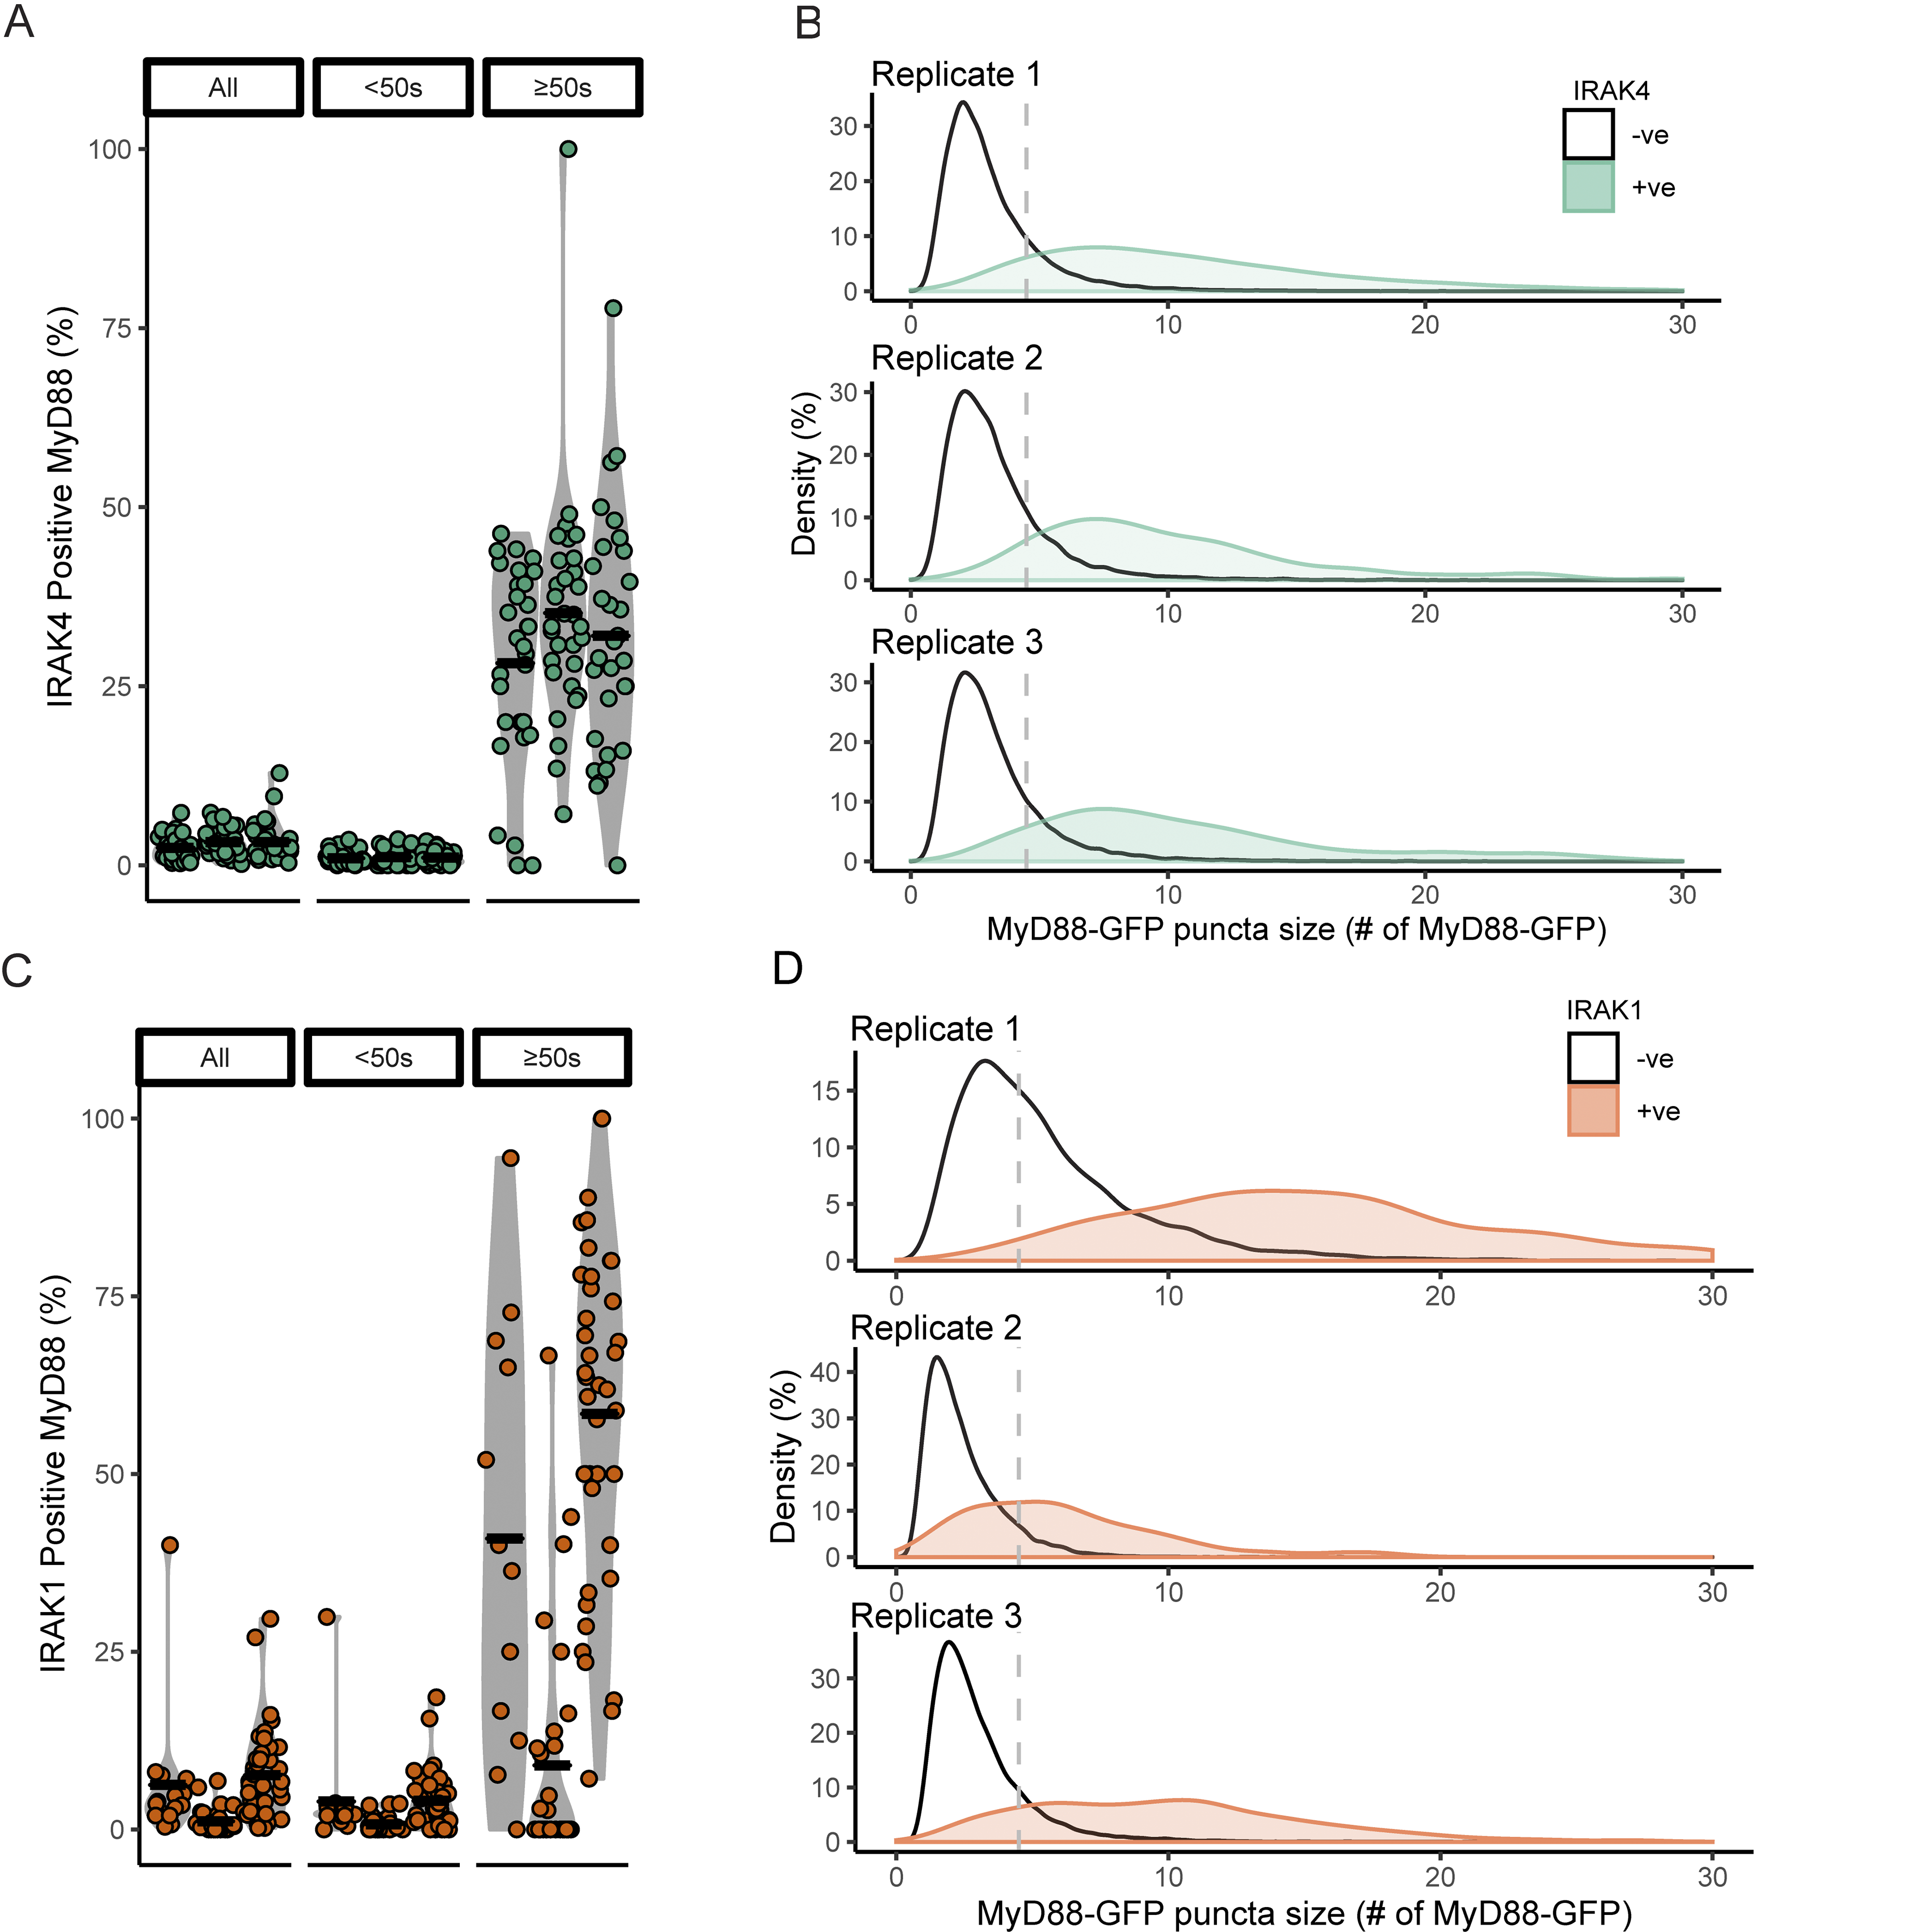
\includegraphics[width=\textwidth, height=\textheight, keepaspectratio]{jcb/figs4.png}}}
\captionsetup{parbox=none}
\captionof{figure}[Analysis of MyD88-GFP and IRAK4/1-mScarlet colocalization]{\textbf{Analysis of MyD88-GFP and IRAK4/1-mScarlet colocalization.}
\vspace{1em}
\\
(A-D) Data shown from clonal MyD88-GFP/IRAK4-mScarlet--expressing EL4 cells (green, A and B) or IRAK1-mScarlet (orange, C and D).
\vspace{1em}
\\
(A and C) Data points are the proportion of individual cells from independent experiments. Bars are experimental replicate means.
\vspace{1em}
\\
(B and D) Vertical line in B and D is at 4.5\times MyD88-GFP.
\vspace{1em}
\\
(A) Percentage (\%) of MyD88-GFP puncta that colocalizes with IRAK4-mScarlet, combined, and by MyD88-GFP lifetime (less than 50 seconds or at least 50 seconds) per cell across experimental replicates. Violin plot of the percent of MyD88-GFP puncta that is colocalized with IRAK4-mScarlet, combined, and categorized by lifetime (less than 50 seconds or at least 50 seconds). Few tracks recruit IRAK4 (“All”, n = cells, replicates 1--3: 2.4\%, n = 30; 3.2\%, n = 31; 3.3\%, n = 30). It is especially evident in MyD88-GFP puncta that persist for less than 50 seconds (“less than 50 seconds”, n = cells, replicates 1--3: 1.0\%, n = 30; 1.2\%, n = 31; 1.1\%, n = 30). However, MyD88-GFP puncta that persist for at least 50 seconds are more likely to recruit IRAK4 (“ $\geq$50 seconds”, n = cells, replicates 1--3: 28\%, n = 30; 35\%, n = 31; 32\%, n = 30).
\vspace{1em}
\\
(B) Maximum MyD88-GFP size of IRAK4-mScarlet colocalized and noncolocalized puncta across experimental replicates. Density plot of MyD88-GFP size categorized as colocalized (green) or noncolocalized (black) with IRAK4-GFP. MyD88-GFP puncta colocalized with IRAK4-mScarlet are brighter (mean colocalized versus not colocalized, n = puncta, replicates 1--3: 11\times MyD88-GFP, n = 835 versus 3.1\times MyD88-GFP, n = 29,072; 10\times MyD88-GFP, n = 601 versus 3.3\times MyD88-GFP, n = 17,221; 11.7\times MyD88-GFP, n = 552 versus 3.3\times MyD88-GFP, n = 17,854).
\vspace{1em}
\\
(C) Percentage (\%) of MyD88-GFP puncta that colocalize with IRAK1-mScarlet, combined and by MyD88-GFP lifetime (less than 50 seconds or at least 50 seconds) per cell across experimental replicates. Few tracks recruit IRAK1 (“All”, n = cells, replicates 1--3: 6.3\%, n = 15; 1.5\%, n = 32; 7.6\%, n = 40). It is especially evident in MyD88-GFP puncta that persist for less than 50 seconds (“less than 50 seconds”, n = cells, replicates 1--3: 3.9\%, n = 15; 0.74\%, n = 32; 4.1\%, n = 40). However, MyD88 puncta that persist for at least 50 seconds are more likely to recruit IRAK1 (“ $\geq$50 seconds”, n = cells, replicates 1--3: 41\%, n = 15; 9.0\%, n = 32; 59\%, n = 40).
\vspace{1em}
\\
(D) Maximum MyD88-GFP size of IRAK1-mScarlet colocalized and non-colocalized puncta across experimental replicates. Density plot of MyD88-GFP size categorized as colocalized (orange) or not colocalized (black) with IRAK1-GFP. MyD88-GFP puncta colocalized with IRAK1-mScarlet are brighter (mean colocalized versus not colocalized, n = puncta, replicates 1--3: 19\times MyD88-GFP, n = 291 versus 5.6\times MyD88-GFP, n = 5,401; 6.2\times MyD88-GFP, n = 314 versus 2.4\times MyD88-GFP, n = 14,125; 10\times MyD88-GFP, n = 1,439 versus 3.1\times MyD88-GFP, n = 16,834). -ve, negative; +ve, positive; MW, molecular weight.
\vspace{1em}
\\
(A-D: Images acquired by Fakun Cao and the thesis author. Analysis, plots by the thesis author. Figure, descriptions extracted from \autocite{Deliz-Aguirre_2021}.)}
\label{p1:S4}
\end{centering}

\section{IRAK4 regulates MyD88 oligomer size}
\sectionmark{IRAK4 regulates MyD88}
\begin{centering}
\centering{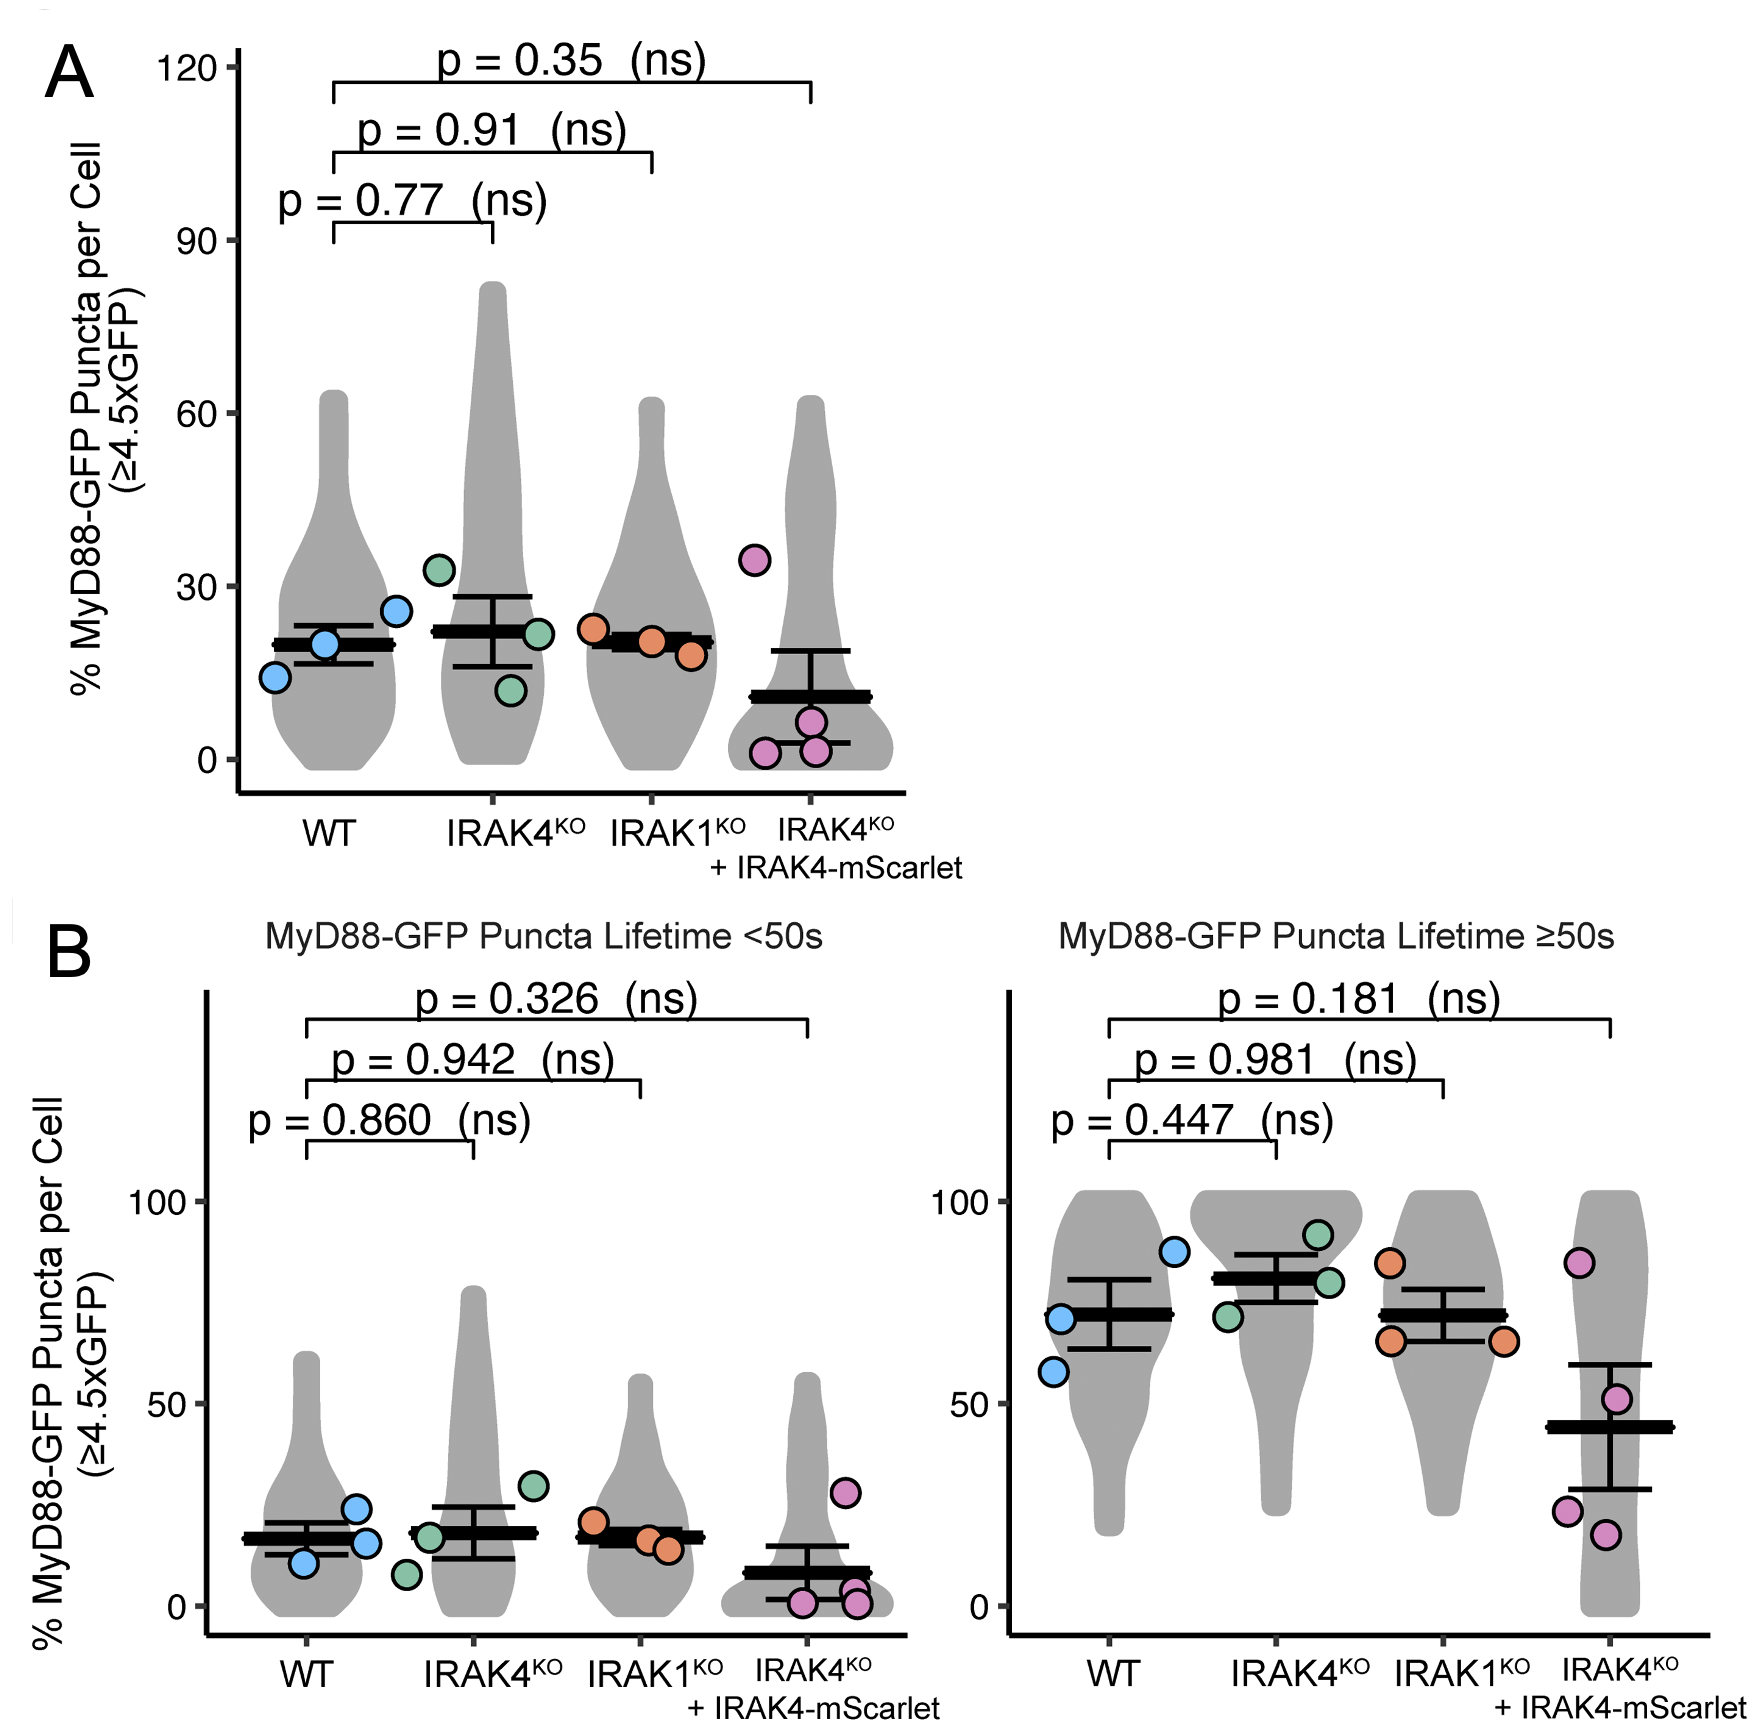
\includegraphics[width=\textwidth, height=\textheight, keepaspectratio]{jcb/figs5a.png}}
\captionsetup{parbox=none}
\captionof{figure}[MyD88-GFP dynamics in KO cell lines]{\textbf{MyD88-GFP dynamics in KO cell lines.}
\vspace{1em}
\\
(A) The percentage per cell of large MyD88 oligomers in WT, IRAK4 KO, and IRAK1 KO EL4 cell lines. Quantification of the percentage (\%) per cell of MyD88-GFP puncta with a maximum intensity at least 4.5\times GFP. Violin plots show the distribution of the cell data. Data points superimposed on violin plots are the averages of independent experimental replicates. Bars represent mean ± SEM (n = 3 or 4 experimental replicates, with more than 10 cells measured per replicate).
\vspace{1em}
\\
(B) The percentage per cell of large MyD88 oligomers is equivalent for short- and long-lived MyD88-GFP puncta across WT and KO cell lines. Quantification of the proportion (\%) per cell of MyD88-GFP puncta with a maximum intensity of at least 4.5\times GFP categorized by lifetimes of less than 50 seconds or at least 50 seconds. Violin plots show the distribution of the cell data. Data points superimposed on the violin plots are the averages from independent experiments. Bars represent mean ± SEM (n = 3 or 4 experimental replicates, with >10 cells measured per replicates). WT and KO image means were compared using an unpaired Student's t test.
\vspace{1em}
\\
(A-B: Images acquired by Fakun Cao and the thesis author. Analysis, plots by the thesis author. Figure, descriptions extracted from \autocite{Deliz-Aguirre_2021}.)}
\label{p1:S5}
\end{centering}

\chapter{Supplemental: The IL-1 pathway circuitry has coupled signalosomes with feedback loops}
\chaptermark{Supplement: IL-1 pathway circuitry}
This supplement offers experiment rationale, more details on the methodology, and findings to support the findings shown in Results~\ref{chapter:p2}.

\section{The IL-1 pathway proteins assemble sequentially}
\label{section:sequential}
\sectionmark{Sequential assembly}
To determine the assembly sequence, I had previously measured when IRAK4/1 reached 1\times (see Results~\ref{section:IRAK_recruitment}). However, this would mean relying on the fluorophore calibration. Here, a different approach was selected to identify the assembly sequence, independent of signal calibrations.

I undertook a series of steps: (1) subtract the lowest intensity thereby assigning a value of 0\% to the minimum intensity, (2) divide by the highest intensity, assigning a value of 100\% to the maximum intensity, and (3) identify when 50\% is reached. This approach rescales all intensities from 0\% to 100\% in the intensity over time plot, with the time value selected when the puncta reaches a rescaled intensity of 50\%. The benefit of this approach is its insensitivity to calibration values. One could argue that the maximum oligomer size (scaled intensity of 100\%) is preferable. However, the signal had more variability at later time points. Thus, the assembly midpoint (50\%, as indicated in line plot, Fig.~\ref{p2:1a}A) was used. Microbial growth laws, commonly employed to determine the rate of microbial growth, also use the midpoint (50\%) approach, termed mid-log phase. In short, the midpoint offered numerous advantages, namely less variability and no reliance on the calibration.

One limitation of this approach is the potential introduction of artifacts through the averaging of puncta. Individual puncta might behave differently than the average (see Fig.~\ref{p2:D1}). Yet, a similar approach is undertaken in microbiology. Growth dynamics are measured based on measuring the optical density of the entire test tube, and not the doubling rate of individual bacterium. Despite its limitations, the average measurement provides a useful rough estimate of assembly order (Fig.~\ref{p2:1a}A), which is further substantiated by other measurements presented in this study. To measure trends better, the intensities were slightly smoothed using a Savitzky-Golay filter to remove noise. They were then visually inspected to ensure similarity between the smoothed and original curves.

Like in bacterial growth curves, it was observed that puncta intensities over time appeared to follow a sigmoidal function (most dramatically seen in NEMO), characterized by slow starting growth, rapid mid-phase growth, and a plateau phase at the end (Fig.~\ref{p2:1a}B). The MyD88 intensities (black) showed an intensity decrease after reaching the plateau, suggesting potential disassembly (Fig.~\ref{p2:1a}B). This will be investigated later in Results~\ref{section:disassembly_results}.

\section{Individual puncta show heterogeneous temporal dynamics}
\sectionmark{Individual heterogeneity}
Structural methods \autocite{Lin_2010} cannot capture the heterogeneity in protein signaling dynamics. Yet the heterogeneity is important in IL-1 signaling to initiate a cellular response \autocite{DeFelice_2019}. This study examined protein puncta and showed highly heterogeneous dynamics (Fig.~\ref{p2:D1}), perhaps because proteins are probing the IL-1 induced nucleation site. To investigate this, I evaluated when each protein in individual puncta reached mid-assembly (as described in Appendix~\ref{section:sequential}), defining the assembly midpoint times for MyD88 (green) and the downstream proteins (magenta) (Fig.~\ref{p2:D1}A). By subtracting the MyD88 assembly midpoint time from the downstream protein assembly midpoint time, I established the $t_{50\%\text{ assembly}}$ parameter. 
\begin{equation*}
t_{50\%\text{ assembly}} = \text{Downstream Protein } t_{50\%\text{ assembly}} - \text{MyD88 }t_{50\%\text{ assembly}}
\end{equation*}
A positive value indicates MyD88 reaches mid-assembles first, whereas a negative value indicates the downstream protein reaches mid-assembly first (Fig.~\ref{p2:D1}A-B). Mid-assembly timepoints are informative of the final assembly state. Based on this, I hypothesized that the assembly order inferred from the averages of all puncta (Fig.~\ref{p2:1a}B) should be comparable to the order obtained by averaging mid-assembly timepoints of individual puncta (Fig.~\ref{p2:D1}A-B), and anticipate that on average, MyD88 assembles first.

The mid-assembly time difference between proteins is depicted in a density plot (Fig.~\ref{p2:D1}A-B). For most cell lines, MyD88 reached mid-assembly first, with the exception of the MyD88-IRAK4 cell line, where both proteins reached mid-assembly almost simultaneously. It is known that MyD88 and IRAK4 are part of the Myddosome complex \autocite{Lin_2010}, with IRAK4 appearing approximately 14 seconds after MyD88 (Results~\ref{chapter:p1}). Unlike the temporal resolution of Results~\ref{chapter:p1} at 1 Frame Per Second, Results~\ref{chapter:p2} had a 0.25 Frames Per Second (FPS) temporal resolution which is limiting, only capturing a relatively small percentage of data when MyD88 recruits IRAK4. The findings suggest that the pipeline can detect transient, heterogeneous puncta, which could serve a biological purpose, such as proteins sampling the plasma membrane and binding only after certain conditions are met. In a broader context, these observations of heterogeneous dynamics highlight the significance of analyzing individual puncta dynamics, as bulk analysis might conceal such dynamic information.


\begin{centering}
\centering{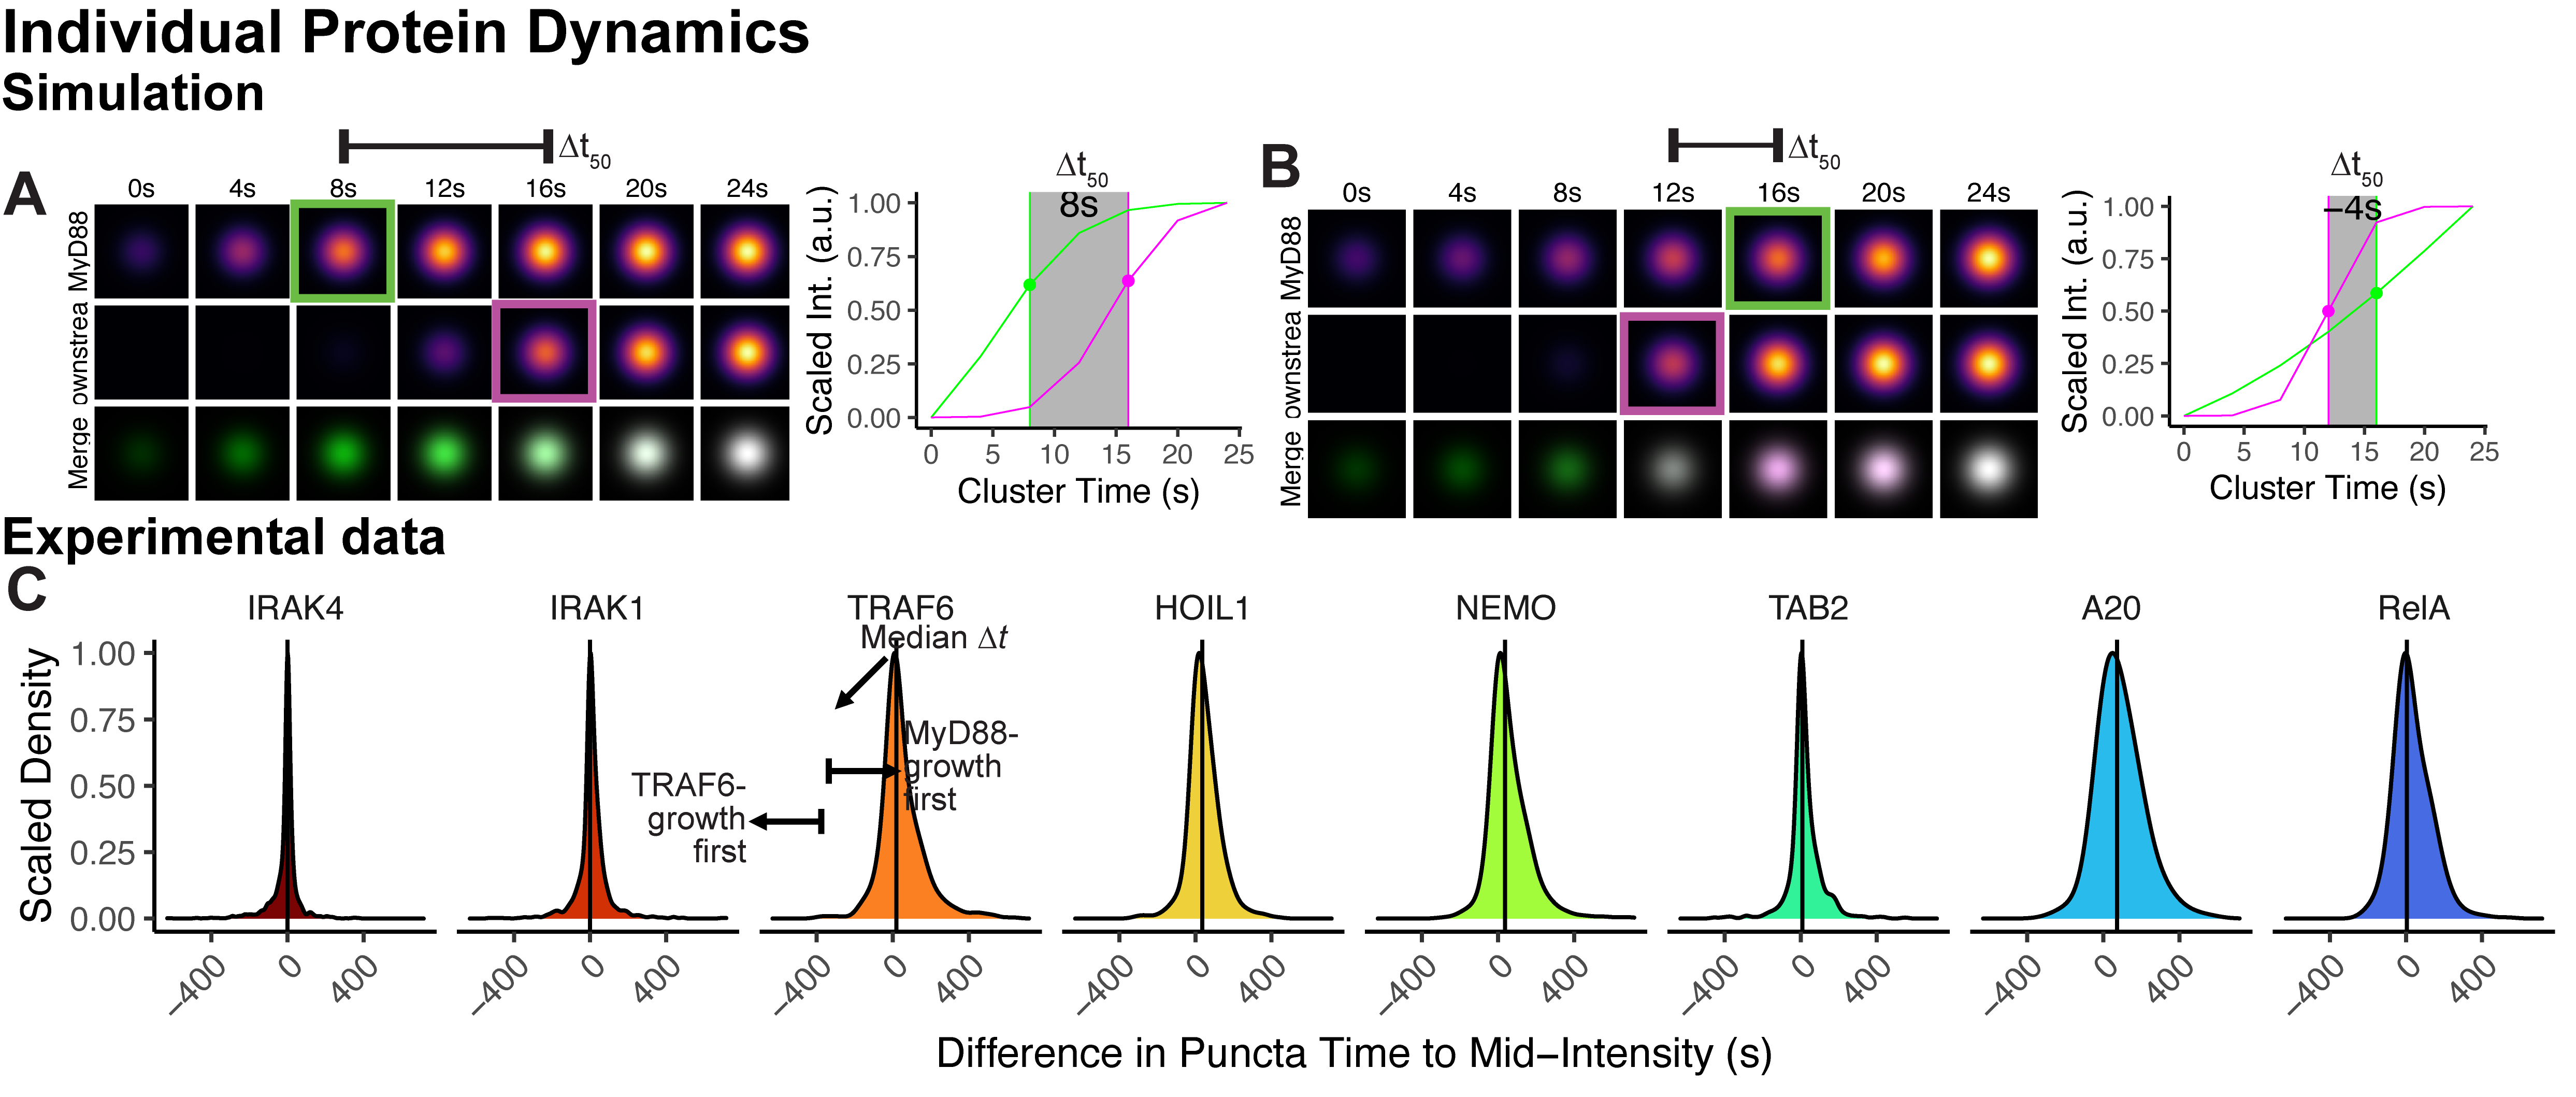
\includegraphics[height=\textwidth, width=\textheight, angle=-90, keepaspectratio]{mod/figD1.png}}
\captionsetup{parbox=none}
\captionof{figure}[Individual puncta assemblies reveal highly dynamic IL-1 pathway proteins]{\textbf{Individual puncta assemblies reveal highly dynamic IL-1 pathway proteins.}
\vspace{1em}
\\
(A-B) Montage of simulated puncta showing MyD88-growth first (A) and downstream-protein-growth first (B). Time traces of these puncta are shown to the right, with a MyD88 simulation in green and the downstream protein simulation in magenta. Boxes indicate where mid-assembly (50\% of max intensity) is reached. Next, the 50\% assembly timepoint is identified (box in montage, dot in time-trace). The time difference between the downstream protein and MyD88 is calculated for each puncta.
\vspace{1em}
\\
(C) This density plot illustrates the frequency of individual puncta time-differences in mid-intensity times. The mid-intensity time difference approach was chosen due to the heterogeneous colocalization sizes of individual puncta. A blanket size threshold would not capture growth dynamics as effectively. The high degree of heterogeneity forms the basis for using other approaches to examine colocalization dynamics.
\vspace{1em}
\\
(C: Imaging data courtesy of Fakun Cao, Niranjan Srikanth, Elba del Val and Claudia Abad-Baucells. Analysis, plots by the thesis author.)}
\label{p2:D1}
\end{centering}

\section{Variance propagates consistently with average measurements}
\label{section:propagation}
\sectionmark{Variance propagation}
I previously measured the protein assembly order using the time to mid-assembly of median curves (Fig.~\ref{p2:1a}C). However, since the IL-1 signaling pathway protein assembly is assumed to be sequential \autocite{Deliz-Aguirre_2021}, another approach would be to compare the variance at mid-assembly. In sequential assembly, variance is expected to propagate because like a relay, the delay in the recruitment of one protein leads to successive proteins to be delayed. Variance propagation is illustrated in Fig.~\ref{p2:D2}A. Assuming the assembly midpoint difference between IRAK4 and MyD88 is 7$\pm$5 seconds, and IRAK1 and MyD88 is 14$\pm$10 seconds, then the predicted IRAK1-MyD88 assembly midpoint time difference should be 21$\pm$22 seconds (Fig.~\ref{p2:D2}A).

For the experimental data, the measurements were first filtered to ensure that all puncta have a maximum size of at least 1\times MyD88 and 1\times downstream protein. To reduce noise and remove intensity fluctuations that could potentially skew the data, a Savitzky-Golay filter was employed to smooth the data, akin to the method used in Fig.~\ref{p2:1a}. Following this, the assembly midpoint was identified for all proteins. Then, the median absolute deviation was used as a measurement of variance. I observed that the variance accumulates proportionate to how downstream it is (Fig.~\ref{p2:D2}), consistent with the average Fig.~\ref{p2:1b}B and Fig.~\ref{p2:D1}.

The puncta colocalization time has been measured for both, the bulk of puncta and in individual puncta. They are self consistent. However, the requirements for colocalization remain unknown. Next, I will explore the lifetime and max oligomer size thresholds using a similar approach as before (see Results~\ref{chapter:p1}).


\begin{centering}
\centering{\includegraphics[width=\textwidth, height=\textheight, keepaspectratio]{mod/figD2.png}}
\captionsetup{parbox=none}
\captionof{figure}[Variance propagates consistent with the mid-assembly time]{\textbf{Variance propagates consistent with the mid-assembly time.}
\vspace{1em}
\\
(A) Greater variance is expected further downstream due to variance propagation. The ideal scenario depicted here demonstrates how variance theoretically propagates. In this hypothetical case, there is a mid-intensity time difference of 7$\pm$5 seconds between MyD88 and IRAK4, and 14$\pm$10 seconds between IRAK4 and IRAK1. Thus, a delay of 21$\pm$22 seconds should occur between the hypothetical MyD88 and IRAK1 growth.
\vspace{1em}
\\
(B) The variance in mid-intensity time difference from least to most variance is: IRAK4, TAB2, IRAK1, HOIL1, TRAF6 and NEMO, RelA, and A20.
\vspace{1em}
\\
(B: Imaging data courtesy of Fakun Cao, Niranjan Srikanth, Elba del Val Oriza and Claudia Abad-Baucells. Analysis, plots by the thesis author.)}
\label{p2:D2}
\end{centering}

\section{Long-lived, large MyD88 assemblies are more likely to recruit downstream proteins}
\sectionmark{Long-lived, large recruit}
In Results~\ref{chapter:p1}, I showed that when MyD88 puncta last longer ($\geq$ 50 seconds) and when the MyD88 oligomer size is larger (at least 4.5\times), the recruitment of IRAK4 and IRAK1 by MyD88 is improved (see Fig.~\ref{p1:4b}). However, these long-lived large MyD88 puncta were less common (see Fig.~\ref{p1:3b}).

It remains unknown whether these requisite MyD88 properties apply to other proteins within the IL-1 pathway. I hypothesize that like in Results~\ref{chapter:p1}, specific properties of MyD88 puncta, namely lifetime and max oligomer size, influence MyD88’s ability to recruit downstream pathway proteins. I also anticipate that, like Results~\ref{chapter:p1}, the majority of the MyD88 puncta within the new cell lines are short-lived and dim. 

To study the size and lifetime thresholds in IL-1 signaling, I will modify the thresholds because our recent findings showed that Myddosome merging enhances the recruitment of TRAF6, HOIL1, and NEMO \autocite{Cao_2023}. Here (Results~\ref{chapter:p2}), long-lived means the puncta persisted for at least 100 seconds, and large means the puncta has at least 6\times MyD88-GFP.

For each punctum, I plotted the puncta lifetime on the x-axis, and the maximum protein size on the y-axis (Fig.~\ref{p2:S1}A, left). Then, I used a two-dimensional (2D) density plot to visualize the frequency at each xy intersection in color (Fig.~\ref{p2:S1}A, center). The darker purple shades indicate frequent events while lighter yellow events are less frequent events. I added a vertical line to indicate the lifetime threshold, and a vertical line to indicate the max size thresholds (with 2\times for the downstream protein) (Fig.~\ref{p2:S1}A, center). The categorization of these puncta is denoted in Fig.~\ref{p2:S1}A to the right.

To evaluate the requirements for colocalization, I subset the data using 2\times for the downstream protein when evaluating MyD88 size properties (Fig.~\ref{p2:S1}B, left), and 6\times MyD88 when evaluating the downstream protein properties (Fig.~\ref{p2:S1}B, right). Thus, there are a total of six 2D density plots per cell line (Fig.~\ref{p2:S1}C-D). In each 2D density plot, a cyan dot indicates the median average of size and lifetime (Fig.~\ref{p2:S1}C-D).

In all plots, we can see the broad distribution of puncta lifetime and MyD88 size, showing that they are heterogeneous (Fig.~\ref{p2:S1}C). On Fig.~\ref{p2:S1}C “All’, we see the cyan dot lying inside the short dim box at the bottom-left, indicating that most MyD88 puncta are small and short-lived (Fig.~\ref{p2:S1}C, “All”). When I subset the data to include at least 2\times downstream protein, we see the cyan dot shift towards the long-lived bright box at the top-right, indicating that downstream protein recruitment by MyD88 is enhanced by long-lived puncta and bright MyD88 (Fig.~\ref{p2:S1}C, “+ Coloc. ($\geq$2\times Downstr. Prot.)”). We can also observe that bright and long-lived appear correlated, as indicated by the diagonal distribution of the frequency (Fig.~\ref{p2:S1}C, “+ Coloc. ($\geq$2\times Downstr. Prot.)”).

I then evaluated the distribution of downstream protein size and puncta lifetime. NEMO and RelA appeared at the plasma membrane transiently. Thus, based on visual inspection of the images, I expect these two proteins to appear larger than the rest of the downstream proteins, but still short-lived. The density plot showed that most downstream proteins are smaller than 2\times and live under 100 seconds (Fig.~\ref{p2:S1}D, “All”). Consistent with the visual inspection, NEMO and RelA were the exceptions, forming structures larger than 1\times (Fig.~\ref{p2:S1}D, “All”). When evaluating only complexes with large MyD88, we can see puncta are longer lived and enriched in the downstream protein (Fig.~\ref{p2:S1}D, “+ Coloc. ($\geq$6\times MyD88)”). This indicates that downstream proteins oligomerize inducibly, dependent on long-lived large MyD88.



\begin{centering}
\bigfig{\centering{\includegraphics[height=\textwidth, width=\textheight, keepaspectratio]{mod/figS1.png}}}
\captionsetup{parbox=none}
\captionof{figure}[The relationship between lifetime, maximum oligomer size and colocalization for the IL-1 pathway protein dynamics]{\textbf{The relationship between lifetime, maximum oligomer size and colocalization for the IL-1 pathway protein dynamics.} Previously, I analyzed the average behavior of puncta and examined protein growth in individual puncta. However, these approaches focused on averages, not the spread of the data. 
\vspace{1em}
\\
(A) To explore the relationship between lifetime, maximum oligomer size, and colocalization, I calculated the lifetime and maximum oligomer size for individual puncta. A one-dimensional (1D) representation of this data would be a histogram, as shown on the left. The intersection of these two variables can be plotted in two dimensions (2D), with frequency represented by color. The data can be divided into quadrants based on lifetime (threshold = 100 s) and brightness (threshold = 6\times for MyD88 and 2\times for the downstream protein). This division can be conceptualized as a 2\times2 contingency table, commonly used in epidemiological studies. Summarizing a continuous variable into a binary variable simplifies the data, making it easier to draw conclusions.
\vspace{1em}
\\
(B) I plotted the data as-is (“All”) and also sorted it based on colocalization status, using 6\times as the MyD88 threshold and 2\times as the downstream protein size threshold.
\vspace{1em}
\\
(C) The MyD88 “All” data indicates that most puncta are small and short-lived. Due to the similarity between “All” and “- colocalization,” I concluded that most puncta are small and short-lived, which aligns with my previous findings \autocite{Deliz-Aguirre_2021}. However, when the data is filtered to include only puncta with a maximum downstream protein size exceeding the 2\times threshold (“+ colocalization”), it becomes evident that size and lifetime requirements exist for binding downstream proteins.
\vspace{1em}
\\
(D) Conversely, I examined the dynamics of the downstream protein. Most puncta contain few or no downstream proteins (“All”). The same is true for complexes with less than 6\times MyD88 (“- Colocalization”). Interestingly, NEMO and RelA exhibit some activity even in puncta with <6\times MyD88, which corroborates my visual examination of the images. NEMO and RelA are present at the plasma membrane, even without MyD88. Focusing only on large ($\geq$) MyD88 structures, I observed long-lived, large downstream proteins. From this analysis, I concluded that lifetime and size are crucial criteria for the colocalization of proteins.
\vspace{1em}
\\
(C-D: Imaging data courtesy of Fakun Cao, Niranjan Srikanth, Elba del Val Oriza and Claudia Abad-Baucells. Analysis, plots by the thesis author.)}
\label{p2:S1}
\end{centering}

\section{Colocalization has size thresholds}
\label{section:thresholds}
\sectionmark{Colocalization thresholds}
To measure the lifetime and size properties of MyD88, I used 2\times2 tables. The application of 2\times2 tables in epidemiological studies is extensive, as demonstrated by the COVID-19 pandemic where multiple testing methods were available, including the gold-standard PCR tests and the cheaper antigen tests. The effectiveness of these antigen tests was scrutinized by comparing the antigen test result (positive or negative) against PCR tests. This binary categorization enabled epidemiologists to calculate the sensitivity and specificity rates, the positive predictive value, and the negative predictive value of the antigen tests. Employing a similar approach to analyze MyD88 properties, 2\times2 tables were used to establish the relationship between two variables---maximum and lifetime size (example on Fig.~\ref{p2:S2}A). Using this statistical tool, the data was binarized\footnote{Split into two categories}, making trends easier to identify, and thus, facilitating conclusions. In Fig.~\ref{p2:S2}, size and lifetime were used as features\footnote{Piece of information with properties that facilitate characterization} for analysis using dimensionality reduction (Fig.~\ref{p2:S2}A, concept explained in Methods~\ref{section:complex}). The thresholds remained unchanged from the previous section (Fig.~\ref{p2:S2}A and B, respectively).

Most events were short-lived and dim across all proteins (Fig.~\ref{p2:S2}C, center box “short-lived, dim”). Intriguingly, the next most frequent puncta bin was long-lived and bright (Fig.~\ref{p2:S2}C, top-left box “long-lived, bright”), suggesting a switch-like behavior transitioning from an unstable transitory complex to a steady state. The total sample size (N) for this analysis is denoted at the bottom right corner of Fig.~\ref{p2:S2}C. Next, I evaluated if this switch-like behavior is associated with the presence of downstream proteins in the puncta.


\begin{centering}
\bigfig{\centering{\includegraphics[height=\textwidth, width=\textheight, angle=-90, keepaspectratio]{mod/figS2.png}}}
\captionsetup{parbox=none}
\captionof{figure}[Analysis of IL-1 pathway protein colocalization reveals MyD88 size thresholds preferred over lifetime thresholds]{\textbf{Analysis of IL-1 pathway protein colocalization reveals MyD88 size thresholds preferred over lifetime thresholds.} I extracted the lifetime and maximum MyD88 size for individual puncta.
\vspace{1em}
\\
(A) Continuous variables were converted into binary variables using 100 seconds and 6\times thresholds, respectively. Puncta were classified as short-lived if their duration was under 100 s, and long-lived if they persisted for at least 100 seconds. Additionally, puncta were categorized as dim if they were under 6\times MyD88, and bright if they had at least 6\times MyD88. The 2\times2 contingency table is shown here.
\vspace{1em}
\\
(B) Colocalization was defined at least 2\times downstream protein size.
\vspace{1em}
\\
(C) I calculated the proportion of puncta meeting the long/short-lived and bright/dim criteria, and also displayed the actual N in the “Total.” Most puncta are short-lived and dim. These values are slightly skewed because puncta must have persisted for at least 44 seconds (11 frames) to be included in the analysis. Bars indicate median. Error bars indicate median absolute deviation.
\vspace{1em}
\\
(D) I also examined the proportion of puncta with a maximum downstream protein size of at least 2\times. I had established that most puncta are short-lived and dim, yet the proportion of long-lived, bright events was significantly enriched when examining colocalized MyD88 puncta. Among long-lived and bright puncta, colocalization is more likely with bright puncta. This finding indicates that there are MyD88 size thresholds, rather than time thresholds, for colocalization. Bars indicate median. Error bars indicate median absolute deviation.
\vspace{1em}
\\
(E) The best predictor of colocalization is assembly size. Larger assemblies are more likely to colocalize. This effect is enhanced with longer lifetimes.
\vspace{1em}
\\
(C-D: Imaging data courtesy of Fakun Cao, Niranjan Srikanth, Elba del Val Oriza and Claudia Abad-Baucells. Analysis, plots by the thesis author.)}
\label{p2:S2}
\end{centering}

Based on the established crystal structures \autocite{Lin_2010}\autocite{Ye_2002} and our previous work \autocite{Cao_2023}\autocite{Deliz-Aguirre_2021}, I hypothesized that the recruitment of downstream proteins must meet stoichiometric (size) requirements, suggesting the presence of size thresholds. I used the same thresholds (Fig.~\ref{p2:S3}A) and colocalization definitions (Fig.~\ref{p2:S3}B) as before. I measured the relative proportion of colocalization using the percentage of events that colocalized as a metric (Fig.~\ref{p2:S3}B). Despite being further downstream, I expected NEMO and RelA to have a higher colocalization tendency because of the observations in Fig.~\ref{p2:S1}D. I also hypothesized that an assembly order could be inferred by a decreasing colocalization percentage. This is because the further downstream, the longer the mid-assembly time point (Fig. ~\ref{p2:1b}B), and thus, a longer lifetime (stable complex) is required to successfully recruit downstream proteins.

As anticipated, the IRAK4/1 data (Fig.~\ref{p2:S3}C, top-left) aligned with previous findings in that there are lifetime and size thresholds \autocite{Deliz-Aguirre_2021}. NEMO and RelA exhibited higher colocalization rates, as expected, but an enrichment in colocalization was observed for long-lived and especially bright NEMO and RelA, corroborating the requisite threshold model. Requisite MyD88 lifetime and size properties were observed in other downstream proteins of the IL-1 pathway. However, when comparing the “long-lived, dim” and “short-lived, bright” categories, most puncta preferred to be short-lived and bright, suggesting a size threshold being more likely than a lifetime threshold when it comes to downstream protein recruitment by MyD88 (Fig.~\ref{p2:S3}C). I also observed that the colocalization percent (Fig.~\ref{p2:S3}C) and mid-assembly times (Fig. ~\ref{p2:1b}B) correlate, further substantiating the sequential assembly.

In summary, the analysis supports a requisite size threshold model (Fig.~\ref{p2:S3}C). MyD88 assemblies must surpass a minimum size threshold for the recruitment of downstream proteins, which can be amplified by a longer lifetime (Fig.~\ref{p2:S3}C). Moreover, the dynamics of protein assembly in the IL-1 pathway involve numerous intermediates and exhibit a switch-like behavior transitioning from an unstable to a steady state.


\begin{centering}
\bigfig{\centering{\includegraphics[height=\textwidth, width=\textheight, angle=-90, keepaspectratio]{mod/figS3.png}}}
\captionsetup{parbox=none}
\captionof{figure}[Analysis of IL-1 pathway protein colocalization reveals MyD88 size thresholds preferred over lifetime thresholds]{\textbf{Analysis of IL-1 pathway protein colocalization reveals MyD88 size thresholds preferred over lifetime thresholds.} I extracted the lifetime and maximum MyD88 size for individual puncta.
\vspace{1em}
\\
(A) I also examined the proportion of puncta with a maximum downstream protein size of at least 2\times. I had established that most puncta are short-lived and dim, yet the proportion of long-lived, bright events was significantly enriched when examining colocalized MyD88 puncta. Among long-lived and bright puncta, colocalization is more likely with bright puncta. This finding indicates that there are MyD88 size thresholds, rather than time thresholds, for colocalization. Bars indicate median. Error bars indicate median absolute deviation.
\vspace{1em}
\\
(B) The best predictor of colocalization is assembly size. Larger assemblies are more likely to colocalize. This effect is enhanced with longer lifetimes.
\vspace{1em}
\\
(A: Imaging data courtesy of Fakun Cao, Niranjan Srikanth, Elba del Val Oriza and Claudia Abad-Baucells. Analysis, plots by the thesis author.)}
\label{p2:S3}
\end{centering}

\section{Protein puncta have two different biophysical properties}
\label{section:biophysics}
\sectionmark{Biophysical properties}
Phase separation involves demixing of different molecules leading to the formation of an aggregate known as a condensate. In soft matter physics, diverse forms of condensed matter exist, including polymers, sand, gels, liquid crystals, foams, and polymers. The concept of phase separation has emerged as a mechanism for protein coalescence into larger assemblies, often termed as membraneless organelles \autocite{Hyman_2011}. The Myddosome is a filamentous polymer, and thus, it is a condensate \autocite{Lin_2010}\autocite{O’Carroll_2018}. Given that the puncta dynamics observed in this study appear as punctate condensates, and that the IL-1 ligand inducibly initiates the oligomerization of these condensates, it could be inferred that MyD88 assembly is a type of phase transition. A few years ago, a pivotal study by key figures in the phase separation field suggested fluorescence recovery after photobleaching (FRAP) as a microscopy technique for investigating condensate dynamics \autocite{Alberti_2019}.

To probe the biophysical properties of the IL-1 pathway condensates, Fakun Cao employed FRAP. This was initially applied to Myddosome proteins MyD88, IRAK4 and IRAK1 (Fig.~\ref{p1:5}), which showed no recovery. This observation implies the Myddosome complex is stable and lacks dynamic exchange with its surrounding environment. Similar experiments were repeated for TRAF6 and HOIL1 are shown in Fig.~\ref{p2:3} with conclusions and findings regarding expanded in Results~\ref{section:two_dynamics}.


\begin{centering}
\centering{\includegraphics[height=\textwidth, width=\textheight, angle=-90, keepaspectratio]{jcb/fig5.png}}
\captionsetup{parbox=none}
\captionof{figure}[Myddosomes are highly stable molecular assemblies that do not exchange with uncomplexed MyD88, IRAK4, or IRAK1]{\textbf{Myddosomes are highly stable molecular assemblies that do not exchange with uncomplexed MyD88, IRAK4, or IRAK1.}
\vspace{1em}
\\
(A) TIRF images of MyD88-GFP before and after (0 and 30 seconds) photobleaching. The red box indicates the position of the Myddosomes on which the FRAP beam was focused. The blue box indicates unbleached control. Right: Cropped time series of the photobleached and controlled Myddosomes.
\vspace{1em}
\\
(B and C) TIRF images of MyD88-GFP/IRAK4-mScarlet-- (B) and MyD88-GFP/IRAK4-mScarlet--(C) expressing cells before photobleaching. The green and magenta boxes indicate the position of the IRAK4-mScarlet-- and IRAK1-mScarlet--labeled Myddosome on which the FRAP beam was focused, respectively. The blue box indicates unbleached control. Right: Cropped time series of the photobleached and controlled IRAK4-mScarlet-- (B) or IRAK1-mScarlet-- (C) labeled Myddosome.
\vspace{1em}
\\
(D--F) Normalized recovery curves for MyD88 (n = 61 cells), IRAK4 (n = 22 cells), and IRAK1 (n = 53 cells). All yielded a maximal recovery of <20\% during the 60 s of observation.
\vspace{1em}
\\
(Panels courtesy of Fakun Cao. Figure, descriptions extracted from \autocite{Deliz-Aguirre_2021}.)}
\label{p1:5}
\end{centering}

\section{The two distinct modular dynamics suggest there are two signalosomes in the pathway}
\label{section:dynamics}
\sectionmark{Two dynamics}
\subsection{Building phase portraits}
To study protein colocalization dynamics, I constructed phase portraits. For each punctum, the size of two proteins over time was measured (Fig.~\ref{p2:3a}A, left plot), and these protein sizes were plotted in phase space (Fig.~\ref{p2:3a}A, right plot). This process was repeated for all trajectories (Fig.~\ref{p2:3a}B). At each intersection of protein size pairs, hundreds of puncta were present, as shown in the 2D density plot which contains the event frequencies (Fig.~\ref{p2:3a}C).

The protein sizes ($x$, $y$) were binned in steps of 3\times. For each punctum, the change in intensity was calculated with a window size of eleven frames (44 seconds) (Fig.~\ref{p2:3a}D). This can be expressed as ($\frac{dx}{dt}$, $\frac{dy}{dt}$), where $d$ represents the derivative and $t$ denotes time. For each stoichiometry (xy intersect), the median change in intensity was calculated and indicated in the arrow direction and color. The arrow direction indicates which protein was enriched, and can be calculated applying a function called the two-argument tangent ($\text{atan2}$) to the changes in intensities of the two proteins (formula: $\theta = \text{atan2}(\frac{dy}{dt}, \frac{dx}{dt})$) (Fig.~\ref{p2:3a}D). A schematic is given in Fig.~\ref{p2:3a}E to illustrate the meaning of the arrow direction. If there is exclusively MyD88 growth, the arrow points to the right ($\rightarrow$). When downstream protein growth occurs, and there is no MyD88 growth, the arrow points up ($\uparrow$). Concurrent recruitment of both proteins directs the arrow upwards-right ($\nearrow$). Disassembly reverses the arrow directions; for MyD88, the arrow is $\leftarrow$; for downstream protein disassembly, $\downarrow$; and for both disassembling, $\swarrow$. However, the arrow direction is just a ratio which does not indicate by how much the protein was enriched, that is, it cannot indicate the change in stoichiometry. To calculate the magnitude of the change in intensity, the following formula was applied: $\text{magnitude} = \sqrt{(\frac{dx}{dt})^2 + (\frac{dy}{dt})^2}$. It is important to note that magnitudes are vectors (they do not have a sign). Thus, to ascertain the growth and disassembly rates of the proteins, the angle must be considered. The MyD88 growth rate is obtained by multiplying the magnitude by the cosine of the angle of the arrow, and the downstream protein growth rate by multiplying the magnitude by the sine of the angle of the arrow. A more comprehensive description of this procedure can be found in the Methods~\ref{chapter:PIRATES_PARLEYS}.

With this understanding of how phase portraits are built, the analysis will now be applied to MyD88 against all eight downstream proteins. This will elucidate the relationship between MyD88 and the downstream protein, focusing on stoichiometries and growth rates.


\begin{centering}
\centering{\includegraphics[width=\textwidth, height=\textheight, keepaspectratio]{mod/fig3a.png}}

\captionsetup{parbox=none}
\captionof{figure}[Building and interpreting phase portraits]{\textbf{Building and interpreting phase portraits.} 
\vspace{1em}
\\
(A) Time traces were transformed into phase space, with MyD88 size on the x-axis and downstream protein size on the y-axis. The example shown depicts time through color gradients.
\vspace{1em}
\\
(B) All MyD88-IRAK4 tracks in phase space. Most puncta exhibit MyD88 growth, while some primarily show IRAK4 growth. Only a few recruit both proteins.
\vspace{1em}
\\
(C) Density of tracks in phase space. The farther from the origin (0\times MyD88, 0\times IRAK4), the fewer tracks. To better understand the overall behavior, the data needs to be summarized. In yellow are the most frequent events, and in blue, the least frequent events.
\vspace{1em}
\\
(D) Data in phase space was binned using a step size of three, leading to bins that increase in multiples of three (0\times, 3\times, 6\times, 9\times). The average change in intensity for each bin was calculated using the intensity five frames forward minus five frames backward ($\pm$5 frames, or $\pm$20 seconds). The median intensity change for each bin was plotted as an arrow, with the arrow color indicating the magnitude of growth as an absolute value. To differentiate between growth and disassembly, the arrow angle must be considered.
\vspace{1em}
\\
(E) Arrow angles indicate protein growth or disassembly. A right-pointing arrow signifies MyD88 growth, while an upward arrow indicates downstream protein growth. Conversely, a bottom-left-pointing arrow implies disassembly of both proteins. The arrow angle is calculated using the two-argument tangent (atan2) of the downstream protein and MyD88 change in intensity. Further details on this calculation can be found in Methods~\ref{chapter:PIRATES_PARLEYS}.
\vspace{1em}
\\
(A-D: Imaging data courtesy of Niranjan Srikanth. Analysis, plots by the thesis author.)}
\label{p2:3a}
\end{centering}

Because of the solved crystal structure \autocite{Lin_2010}, my hypothesis was that the phase portraits would initially show MyD88 growth ($\rightarrow$) for small downstream protein assemblies located at the bottom of the y-axis. Then, if downstream proteins have MyD88 size thresholds, the phase portrait arrows should start rotating, eventually pointing completely upwards. The inflection point would signify the size threshold. Subsequently, I anticipated growth in the downstream protein, indicated by upward-pointing arrows. Considering downstream proteins likely contain MyD88, these arrows would primarily populate larger MyD88 sizes, that is, they would primarily be located to the right of the x-axis. Upon reaching a stoichiometric ratio high on the y-axis and to the right of the x-axis, I expect these arrows to show minimal growth (small magnitude) because they have reached a state of equilibrium.

The events that follow are intriguing since there is no consensus in the field on whether the IL-1 pathway remains stable or disassembles. If the pathway remains stable, the proteins stay put and converge towards a stability point. However, if disassembly occurs, three scenarios are possible: MyD88 disassembles first, the downstream protein disassembles first, or both proteins disassemble together. Alternatively, instead of disassembly, proteins could break apart, moving outside the z-axis of the TIRF microscope’s field of view and into the cytosol. I plotted the phase portraits of MyD88 against all eight downstream proteins (Fig.~\ref{p2:3}F-G). 

\subsection{The Myddosome signalosome phase portraits}
\subsubsection{The MyD88-IRAK4/IRAK1 phase portrait}
In the absence of IRAK4 (0\times IRAK4 arrows), the arrows pointed to the right, indicating MyD88 grew (Fig.~\ref{p2:3}F). However, there were no upward-pointing arrows (IRAK4 growth) and no distinguishable inflection point (arrow switching directions) that would show upward arrows only, indicating predominant IRAK4 growth. Instead, most arrows pointed up-right, suggesting simultaneous growth of MyD88 and IRAK4.

The IRAK1 phase portrait was similar to IRAK4 (Fig.~\ref{p2:3}F). Compared to IRAK4, IRAK1 assemblies were larger. Both IRAK4 and IRAK1 showed positive feedback relative to MyD88.

\subsubsection{The MyD88-TRAF6 phase portraits}
The phase portrait of TRAF6 resembled that of IRAK4 and IRAK1, but featured diagonal arrows for all assemblies with 3\times TRAF6 which indicate and upward arrows after 6\times TRAF6 (Fig.~\ref{p2:3}F). This could suggest the absence of a fixed size threshold, and instead, MyD88 oligomers could have variable lengths. When MyD88 is large, the growth rate of TRAF6 increases, as indicated by the arrow color and direction. This indicates positive feedback between the two proteins.

I also noticed assemblies of MyD88 larger than 15\times that never recruited TRAF6 (Fig.~\ref{p2:3}F). This phenomenon was not seen in IRAK4 nor in IRAK1. This could indicate that some Myddosomes do not recruit TRAF6, possibly signaling through other pathways such as MAPK.

\subsubsection{The MyD88-TAB2 phase portrait}
The phase portrait of TAB2 mirrors that of TRAF6 in that there appear to be multiple trajectories (Fig.~\ref{p2:3}F). Note that all trajectories above 3\times TAB2 require at least 9\times MyD88 (Fig.~\ref{p2:3}F). This suggests that a MyD88 size threshold might exist before TAB2 can bind.

\subsection{The NF-κB signalosome phase portraits}
\subsubsection{The MyD88-NEMO phase portrait}
The phase portrait of NEMO shows a MyD88 size threshold, around 3-6\times MyD88, and also displays an upper boundary at 9\times MyD88. Like TRAF6 and TAB2, some large MyD88 assemblies recruit no downstream protein (Fig.~\ref{p2:3}G). NEMO also demonstrates its ability to form large structures. At the upper sizes of NEMO, arrows point downwards, with some pointing down-left, indicating a size limit for NEMO.

\subsubsection{The MyD88-HOIL1 phase portrait}
The phase portrait of HOIL1 shows MyD88 growth. When MyD88 reaches 24\times, it begins to incorporate HOIL1, and once it reaches 27\times MyD88 3\times HOIL1, the phase portrait shows almost exclusive HOIL1 growth. Then, the arrows point to the left indicating MyD88 disassembly. Since HOIL1 is still growing, this suggests that HOIL1 molecules remain at the plasma membrane. No HOIL1 structures larger than 9\times HOIL1 were observed, implying that both MyD88 and HOIL1 might have maximum assembly sizes, or in other words, assemblies might have defined stoichiometries or maximum sizes. At 12\times MyD88 6\times HOIL1, the arrow points down-left, suggesting HOIL1 might eventually disassemble, although only one arrow indicated this. The HOIL1 phase portrait provides a clear view of new phenomena: negative regulation and MyD88 disassembly.

\subsubsection{The MyD88-A20 phase portrait}
The phase portrait of A20 resembles that of HOIL1 in that it forms a horizontally flipped c, that is, $\supset$. It also shows a 3\times A20 maximum size. The 0\times MyD88 3\times A20 arrow indicates that both MyD88 and A20 eventually disassemble. This phase portrait demonstrates the ability of my phase portraits to resolve dynamics as small as 3\times molecules with minimal noise (noise would be arrows pointing in random directions).

\subsubsection{The MyD88-RelA phase portrait}
The phase portrait of RelA is similar to A20 and HOIL1 in that there is a boomerang-shaped phase portrait with (1) MyD88 growth, (2) RelA growth, and (3) MyD88 disassembly. RelA is recruited in all MyD88 sizes (0-15\times). At 12\times RelA, MyD88 disassembles. MyD88 never reaches a stoichiometry higher than 15\times MyD88.

\subsection{Overall}
Myddosmoes have been shown to have multiple stable stoichiometries of MyD88, ranging from 6-8\times MyD88 \autocite{Moncrieffe_2020}. Interestingly, the phase portraits show multiple trajectories, corroborating that there might be some flexibility regarding the size thresholds (Fig.~\ref{p2:3b}A-B).

In conclusion, I have observed that the MyD88 kinetics show dependency with the downstream protein oligomer size. In some cases, I observe a positive relationship between these two variables, while in others, we see a negative correlation between MyD88 and the downstream protein. In short, there are two types of feedback, positive feedback in the Myddosome signalosome (IRAK4, IRAK1, TRAF6 and TAB2), and negative feedback for the NF-κB signalosome (NEMO, HOIL1, A20, RelA). This is our second evidence of modularity in the IL-1 signaling pathway.


\begin{centering}
\centering{\includegraphics[width=\textwidth, height=\textheight, keepaspectratio]{mod/fig3b.png}}
\captionsetup{parbox=none}
\captionof{figure}[The IL-1 pathway has distinct signalosomes as revealed by phase portrait analysis of MyD88 and downstream protein growth dynamics]{\textbf{The IL-1 pathway has distinct signalosomes as revealed by phase portrait analysis of MyD88 and downstream protein growth dynamics.} 
\vspace{1em}
\\
(A) Phase portraits of IRAK4, IRAK1, TRAF6, and TAB2 display positive feedback with up-right-pointing arrows.
\vspace{1em}
\\
(B) Phase portraits of NEMO, HOIL1, A20, and RelA exhibit a center-like (“circular”) pattern, indicating sequential MyD88 growth, downstream protein growth, and ultimately, MyD88 disassembly. This pattern is interpreted as negative feedback.
\vspace{1em}
\\
(A-B) Overall, there are two primary categories of phase portraits: positive and negative feedback. These phase portraits suggest the existence of two signalosomes in the IL-1 pathway: the Myddosome signalosome (positive feedback) and the NF-κB signalosome (negative feedback).
\vspace{1em}
\\
(A-B: Imaging data courtesy of Fakun Cao, Niranjan Srikanth, Elba del Val Oriza and Claudia Abad-Baucells. Analysis, plots by the thesis author.)}
\label{p2:3b}
\end{centering}

\section{The signalosomes have assembly stages}
\sectionmark{Assembly stages}
Fig.~\ref{p2:3b} phase portraits illustrate how assemblies behave up to 800 seconds after the first punctum appears (Fig.~\ref{p2:3b}). Yet, how the signaling events unfolded remains unknown because the phase portraits do not explicitly show time. To unravel the sequence of events, I generated multiple phase portraits with different cumulative time cutoffs from when the first spot appeared (Fig.~\ref{p2:S4}A-B). To avoid artifacts, I calculated the fluorophore bleaching rates and limited the plots to 800 seconds (199 frames) per puncta, and up to 1200 seconds (300 frames) since the first spot appeared (details in Methods~\ref{section:PARLEYS}). I predicted assembly steps dominated by the activity of a single protein. As time passed, I anticipated that disassembly would become apparent. 

\subsection{Myddosome signalosome assembly dynamics show positive feedback}
The MyD88-IRAK4 phase portrait shows that MyD88 and IRAK4 have rapid growth at 200 seconds as indicated by the arrow colors (Fig.~\ref{p2:S4}A, up-left 200 s). Over time, the rate decreases. After the 400-second mark, growth substantially slowed down (Fig.~\ref{p2:S4}A, up-left 400 s).

The MyD88-IRAK1 phase portrait shows right-pointing arrows that indicate MyD88 oligomerizes first, followed by IRAK1. Interestingly, the $\le$400 second phase portrait shows an empty region at 24\times MyD88, indicating that some long (27-30\times) MyD88 oligomers have virtually no IRAK1 (less than 1.5\times IRAK1) (Fig.~\ref{p2:S4}A, up-right 400 s). At 600 seconds, we see that long MyD88 oligomers with IRAK1 (Fig.~\ref{p2:S4}A, up-right 600 s). Later timepoints show little to no growth as indicated by the arrow colors, with some arrows pointing down (Fig.~\ref{p2:S4}A, up-right 800s onwards), indicating IRAK1 disassembly.

The MyD88-TRAF6 phase portrait shows mostly MyD88 growth at 200 seconds (Fig.~\ref{p2:S4}A, bottom-left at 200 s), and we can start seeing TRAF6 grow at 400 seconds (Fig.~\ref{p2:S4}A, bottom-left at 400 s). This means MyD88 growth precedes TRAF6 growth, consistent with Fig~\ref{p2:1b}B. At 600-800 seconds, the MyD88-TRAF6 shows no arrows above 15\times MyD88, indicating that some MyD88 do not bind TRAF6 (Fig.~\ref{p2:S4}A, bottom-left at 600 s and 800 s). This empty space was also seen in the MyD88-IRAK1 phase portrait at 400 seconds (Fig.~\ref{p2:S4}A, up-right at 400 s). At around 800 seconds, the phase portrait shows what could be the entire lifecycle of a Myddosome signalosome: (i) left arrows indicating MyD88 growth, (ii) up arrows indicating TRAF6 growth, and (iii) Left arrows, indicating MyD88 disassembly.

The TAB2 phase portraits display only MyD88 growth at 200 seconds (Fig.~\ref{p2:S4}A, bottom-right at 200 s). At 400 seconds, TAB2 begins to be recruited, but these TAB2 assemblies are small at 3\times TAB2 (Fig.~\ref{p2:S4}A, bottom-right at 400 s). At 600 seconds, it is apparent that larger TAB2 (at least 6\times) mainly forms where there is larger MyD88 (at least 9\times) (Fig.~\ref{p2:S4}A, bottom-right at 600 s).

\subsection{NF-κB signalosome assembly dynamics show assembly stages}
The MyD88-NEMO phase portrait shows mainly right arrows indicating mainly MyD88 growth at up to 400 seconds (Fig.~\ref{p2:S4}B, up-left at 200 s and 400 s). Then, at 600 seconds, upward arrows appear, indicating recruitment of NEMO (Fig.~\ref{p2:S4}B, up-left at 600 s). Compared to the Myddosome signalosome phase portraits (Fig.~\ref{p2:S4}A), NEMO growth happens later, consistent with Fig~\ref{p2:1b}B. 

The 600 seconds phase portrait also shows upward arrows at 3-6\times MyD88, indicating NEMO growth. The color at 6\times MyD88 shows that NEMO growth is the fastest at this range (Fig.~\ref{p2:S4}B, up-left 600 s). This demonstrates that NEMO is recruited after crossing a MyD88 threshold, consistent with Figs.~\ref{p2:S1}-~\ref{p2:S3}. At 800 seconds and more, the region above 30\times NEMO continues being populated progressively, indicating NEMO growth. However, arrows begin pointing to the left at 800 seconds, which indicates that MyD88 is leaving (Fig.~\ref{p2:S4}B, up-left at 800 s). At 1000 seconds, we see right pointing arrows which means that NEMO leaves (Fig.~\ref{p2:S4}B). The disassembly of MyD88 in the MyD88-NEMO cell line supports the previous observation in Myddosome signalosomes where it was observed (Fig.~\ref{p2:S4}A). The MyD88-NEMO phase portraits have now shown the entire lifecycle of IL-1 signaling events, starting with (i) MyD88 growth, (ii) NEMO growth, (iii) MyD88 disassembly and (iv) NEMO disassembly (Fig.~\ref{p2:S4}D).

The MyD88-HOIL1 phase portrait shows only right pointing arrows at 200 seconds that indicate MyD88 growth only (Fig.~\ref{p2:S4}B, top-left at 200 s). Then, at 400 we can see arrows pointing up at 6\times MyD88 onwards, which means HOIL1 recruitment and growth (Fig.~\ref{p2:S4}B, top-left at 400 s), consistent with Fig~\ref{p2:1b}B. It also supports that there is a MyD88 size threshold before HOIL1 recruitment,consistent with Figs.~\ref{p2:S1}-~\ref{p2:S3}. At 600 seconds, the arrows point up-left that indicate HOIL1 growth and MyD88 disassembly (Fig.~\ref{p2:S4}B, top-left at 600 s). At 800 seconds and beyond, almost all arrows at 3\times HOIL1 and above are pointing left, meaning MyD88 disassembly in puncta with HOIL1 (Fig.~\ref{p2:S4}B, top-left at 600 s). At 1000-1200 seconds, at 0\times MyD88 3\times HOIL1, when almost all MyD88 is depleted, arrows point down which indicates HOIL1 disassembly (Fig.~\ref{p2:S4}B, top-left at 600 s). This shows that the assembly steps seen with NEMO also apply with HOIL1 (Fig.~\ref{p2:S4}D).

The MyD88-RelA and MyD88-A20 phase portraits are similar to NEMO and HOIL1 (Fig.~\ref{p2:S4}B, bottom row). However, the MyD88 size threshold is less evident in A20 (Fig.~\ref{p2:S4}B, bottom-right).

Interestingly, the NF-κB signalosome dynamics and especially the MyD88-RelA phase portrait has some resemblance to the arrow directions of MyD88-TRAF6, which might indicate that TRAF6 bridges these two signalosomes. A similar trend was observed in the mid-assembly times (Fig.~\ref{p2:1b},~\ref{p2:D1}).

In conclusion, IL-1 signal transduction occurs in steps, as shown across different phase portrait time cutoffs (Fig.~\ref{p2:S4}E). The Myddosome signalosome comes first, followed by the NF-κB signalosome (Fig.~\ref{p2:S4}E). There is growing evidence that the IL-1 pathway disassembles, as MyD88 shrinks in the presence of NF-κB signalosome proteins.


\begin{centering}
\bigfig{\centering{\includegraphics[width=\textwidth, height=\textheight, keepaspectratio]{mod/figS4.png}}}
\captionsetup{parbox=none}
\captionof{figure}[IL-1 pathway signalosomes have assembly stages evident in their distinct temporal dynamics]{\textbf{IL-1 pathway signalosomes have assembly stages evident in their distinct temporal dynamics.}
\vspace{1em}
\\
(A-B) Phase portraits with distinct timepoint cutoffs (facets), with each timepoint indicating the time elapsed since the appearance of the first spot.
\vspace{1em}
\\
(A) The Myddosome signalosome forms within the initial 400 seconds, suggesting the early formation of the Myddosome module.
\vspace{1em}
\\
(B) The NF-κB signalosome forms later, around 600 seconds, with MyD88 binding first followed by the recruitment of HOIL1, NEMO, RelA, and ultimately, A20. The NEMO phase portraits indicate that not all large MyD88 assemblies recruit NEMO, suggesting potential binding to a different pathway.
\vspace{1em}
\\
(C-D) Phase portraits can be employed to identify stages in protein assembly.
\vspace{1em}
\\
(C) The Myddosome signalosome displays initial MyD88 growth (right-pointing arrows, 200 seconds) and subsequent recruitment of Myddosome signalosome downstream proteins (IRAK4, IRAK1, TRAF6, TAB2) (upward-pointing arrows, 400 seconds).
\vspace{1em}
\\
(D) The NF-κB signalosome (NEMO, HOIL1, RelA, A20) exhibits similar dynamics of MyD88 assembly (right-pointing arrows), and downstream protein assembly (upward-pointing arrows) but also demonstrates MyD88 disassembly (left-pointing arrows, 800 seconds).
\vspace{1em}
\\
(E) The phase portrait analysis revealed that there are assembly steps where assemblies grow larger over time. Larger Myddosome signalosome assemblies then recruit the NF-κB signalosome. The appearance of the NF-κB signalosome triggers the disassembly of MyD88.
\vspace{1em}
\\
(A-B: Imaging data courtesy of Fakun Cao, Niranjan Srikanth, Elba del Val Oriza and Claudia Abad-Baucells. Analysis, plots by the thesis author.)}
\label{p2:S4}
\end{centering}

\section{The phase lines show the kinetics of the two modules}
\sectionmark{Module kinetics}   
\label{section:phase_lines}
The phase portraits provide insights into the interaction between two proteins. One challenge reading phase portraits is grasping individual protein dynamics. Individual protein kinetics can be obtained by multiplying the magnitude by the sine or cosine of the angle. But to simplify the visualization of protein kinetics, I used a graphical tool known as a phase line. The phase line is simply a one-dimensional representation of how the arrows in the phase portrait evolve, hence they are sometimes called one-dimensional (1D) phase portraits. In this study, phase lines depict how the growth rate of one protein (y-axis) changes as the amount of a component is kept fixed (x-axis). Growth would be shown as y-axis values above the black line, and disassembly would be shown as y-axis values below the black line. To reduce the number of phase lines shown per plot, the data was collapsed so that kinetics can be studied in the presence ($\geq$3\times in blue) or absence (<3\times in red) of a protein (Fig~\ref{p2:S5}A). For this section, the x-axis is the MyD88 oligomer size, on the y-axis the MyD88 growth rate, and in color, the size of the downstream protein (Fig.~\ref{p2:S5}A). 

\subsection{Distinct module feedback dynamics evident in MyD88 kinetics}
\subsectionmark{MyD88 kinetics}

\subsubsection{MyD88 kinetics relative to its size}
I plotted the phase lines of Myddosome signalosome proteins. As we can see in Fig.~\ref{p2:S5}B, the red phase line is above the black line (positive y-axis values), which means MyD88 grows with small Myddosome signalosome downstream proteins, namely IRAK4, IRAK1, TRAF6 and TAB2. Notice how the further along the x-axis--towards larger MyD88, the faster MyD88 grows because of the positive y-axis values increase. This positive correlation between MyD88 size and MyD88 growth (Fig.~\ref{p2:S5}B diagonal-up shape) indicates positive feedback between MyD88 molecules. Simply put, MyD88 enhances its own recruitment. The blue line in Fig.~\ref{p2:S5}B shows that when other Myddosome signalosome proteins are large ($\geq$3\times), MyD88 growth values remain positive (Fig.~\ref{p2:S5}B, blue line above black line). This means MyD88 continues assembling, even when Myddosome signalosome proteins are large.

In Fig.~\ref{p2:S5}B, we can see that the red line hovers slightly above the black line. This means that when there are small (<3\times) NF-κB signalosome proteins (red line), MyD88 grows (positive y-axis value), though less fast. The diagonal-up trend observed in Fig.~\ref{p2:S5}B remains true here, indicating that the more MyD88, the faster MyD88 grows. The blue line hovers below the black line (Fig.~\ref{p2:S5}B, $\geq$3\times). This means that in the presence of large NF-κB signalosome proteins, MyD88 disassembles (negative y-axis value). We can also observe that MyD88 size (x-axis) and MyD88 kinetics (y-axis) are inversely proportional (diagonal-down trend) and thus they are negatively correlated (Fig.~\ref{p2:S5}B, diagonal-down blue line). This means that large NF-κB signalosome proteins not only trigger MyD88 disassembly, but they also invert the MyD88 growth trends.

While these observations reduced the number of points, they still support the phase portrait data (Fig.~\ref{p2:3b}) in that each module has its own type of feedback. The Myddosome signalosome has positive feedback, and the NF-κB signalosome proteins have negative feedback. Additionally, these findings provide compelling evidence that the recruitment of the NF-κB signalosome triggers the disassembly of the Myddosome signalosome, consistent with Fig.~\ref{p2:S4}.

\subsubsection{MyD88 kinetics relative to downstream protein size}
I then plotted MyD88 growth (y-axis) as a function of the downstream protein size (x-axis), separated by small (<3\times in red) or large ($\geq$3\times in blue) of MyD88 (Fig.~\ref{p2:S5}C). We can see that in all, the red line is hovering slightly above the black line, which means that when MyD88 is under 3\times (red line), there is little to no MyD88 growth (nearing black line) (Fig.~\ref{p2:S5}D).

The blue line shows two broad types of relationships. In the Myddosome signalosome, the blue line is above the black line indicating MyD88 growth in $\geq$3\times MyD88 puncta (Fig.~\ref{p2:S5}D). This is consistent with the positive feedback between Myddosome signalosome proteins. The exception is TRAF6 where the line dips after 6\times TRAF6 (Fig.~\ref{p2:S5}D, third top-down).

In the IRAK4 plot, we see that the more IRAK4 in a puncta, the faster MyD88 grows. This suggests that IRAK4 positively promotes MyD88 growth. However, I also had observed that in the absence of IRAK4, MyD88 grows and makes large MyD88 oligomers (Fig.~\ref{p1:6a}-~\ref{p1:6b}), which would suggest IRAK4 negatively regulates MyD88 size. This indicates that the MyD88-IRAK4 interaction dynamics are complex and nonlinear. Further experimentation would be required to untangle the dynamics.

In the NF-κB signalosome, we see that the blue lines point downwards as more downstream protein is present in the puncta. This indicates that the more NF-κB signalosome protein there is in the puncta, the faster MyD88 disassembles. For HOIL1 and A20 of the NF-κB signalosome, the blue line is diagonal-down indicating that there is a negative correlation between downstream protein size (x-axis) and MyD88 growth rate (y-axis) (Fig.~\ref{p2:S5}D). This means that more downstream protein is associated with a faster MyD88 disassembly rate (Fig.~\ref{p2:S5}D). This trend happens in RelA, though to a lesser extent (Fig.~\ref{p2:S5}D).

\subsection{Downstream protein kinetics show nonlinearity}
\subsectionmark{Downstream protein kinetics}
\subsubsection{Downstream protein kinetics relative to MyD88 size}
Next, I examined the downstream protein kinetics, plotting MyD88 size on the x-axis, downstream protein growth rate on the y-axis, and distinguishing between the absence (<3\times in red) or presence ($\geq$3\times in blue) of the downstream protein (Fig.~\ref{p2:S5}E illustrates this process).

The red line hovers around the black line, irrespective of where the line is along the x-axis (Fig.~\ref{p2:S5}F, red lines). This means that when there is a negligible amount of downstream protein in the puncta (<3\times, red line), the downstream protein growth rate is negligible (values near black line on y-axis), irrespective of MyD88 size (x-axis position).

However, the blue line shows that in IRAK4, TAB2 and RelA, the further along the x-axis, the higher the y-axis value (Fig.~\ref{p2:S5}F, blue lines). This means that for IRAK4, TAB2 and RelA, when there is $\geq$3\times downstream protein (blue line), the more MyD88 (x-axis), the faster these proteins grow (y-axis). Simply put, more MyD88 enhances IRAK4, TAB2 and RelA growth.

In the blue lines of IRAK1, HOIL1 and A20, the further along the x-axis, the lower the y-axis value (Fig.~\ref{p2:S5}F, blue lines). This means that for IRAK1, HOIL1 and A20, when there is $\geq$3\times downstream protein (blue line), the more MyD88 (x-axis), the faster these proteins grow (y-axis). Simply put, more MyD88 leads to IRAK1, HOIL1 and A20 to disassemble. The sigmoidal shape of IRAK4, TAB2, and RelA suggests nonlinear dynamics at play.

The blue line of NEMO is remarkably different to the rest of the proteins. Near the origin (0\times, x-axis), NEMO growth rate is negative (y-axis), but as one moves further along the x-axis, the growth rates shifts closer to 0 molecules per minute until around 12\times MyD88, where NEMO oligomerization becomes positive (Fig.~\ref{p2:S5}F, NEMO blue line). This indicates that NEMO growth relative to MyD88 size is nonlinear. The switch-like behavior would suggest size-dependent dynamics (for example, biphasic regulation), but further experiments and analyses would be needed to confirm this.

\subsubsection{Downstream protein kinetics relative to its size}
The last set of phase lines compare the downstream protein size (x-axis) against the growth rate of the downstream protein (y-axis) with small (<3\times, red line) or large ($\geq$3\times, blue) MyD88 (Fig.~\ref{p2:S5}G).

The red curve was consistently hovering around the black line (Fig.~\ref{p2:S5}H). This means that when puncta have small (<3\times) MyD88, most downstream proteins exhibit no growth. Downstream proteins require a MyD88 size threshold before they can colocalize with MyD88 (Fig.~\ref{p2:3}). Therefore, these puncta with small MyD88 may have virtually no downstream protein.

A notable exception to this trend was NEMO, which had a diagonal-down curve indicating that the more NEMO in complex (x-axis) leads to faster NEMO disassembly (negative y-axis value) (Fig.~\ref{p2:S5}H, NEMO red line). RelA showed a similar trend, though the effect was less noticeable (Fig.~\ref{p2:S5}H, RelA red line). 

The blue curves are generally above the black line, meaning that when there is at least 3\times MyD88 (blue curve), the more downstream protein (x-axis), the faster the downstream protein assembles (y-axis). This is consistent with the requisite size threshold model presented in Figs.~\ref{p2:S1}-~\ref{p2:S3}. The effect is strongest in TAB2, NEMO and RelA. These curves also show a plateau, meaning there is a maximum growth rate. IRAK1 is the exception to the rule. When there is $\geq$3\times MyD88, the more IRAK1 there is in the puncta, the faster IRAK1 disassembles.


\begin{centering}
\bigfig{\centering{\includegraphics[width=\textwidth, height=\textheight, keepaspectratio]{mod/figS5.png}}}
\captionsetup{parbox=none}
\captionof{figure}[Phase lines show that the IL-1 pathway proteins have module-dependent feedback and nonlinearity]{\textbf{Phase lines show that the IL-1 pathway proteins have module-dependent feedback and nonlinearity.} One-dimensional (1D) phase portraits illustrating pathway dynamics. (A, C, E, G) Explanations to how phase lines were constructed. (B, D, F, H) Experimental results. Myddosome signalosome proteins are on the top four rows, and NF-κB signalosome proteins are on the bottom four rows. Points are medians. Point size indicates N.haded region is the standard error of the median.
\vspace{1em}
\\
(A) MyD88 size is in the x-axis, MyD88 growth/disassembly in the y-axis, and in color is the line which indicates kinetics for small (<3\times, red line) or large ($\geq$3\times, blue line) downstream protein (D/S prot.) assemblies.
\vspace{1em}
\\
(B) Myddosome signalosome proteins show MyD88 growth (positive y-axis). More MyD88 in puncta (x-axis) enhances the growth rate. Larger downstream proteins ($\geq$3\times, blue line) reduce the growth rate, except for IRAK4. The NF-κB signalosome proteins show that when they are small (<3\times), MyD88 grows. However, when they are large, MyD88 disassembles (y-axis), especially when there is more MyD88 (right x-axis).
\vspace{1em}
\\
(C) Downstream size is in the x-axis, MyD88 growth/disassembly in the y-axis, and in color is the line which indicates kinetics for small (<3\times, red line) or large ($\geq$3\times, blue line) MyD88 assemblies.
\vspace{1em}
\\
(D) MyD88 growth is slow when there is less than 3\times MyD88 (red line). The Myddosome signalosome proteins show slight growth (positive y-axis) with larger MyD88 ($\geq$3\times, blue line). When there are larger IRAK4 ($\geq$3\times, blue line), MyD88 oligomerization is faster than with smaller IRAK4 (<3\times, red line). The NF-κB signalosome proteins show that in large MyD88 assemblies ($\geq$3\times, blue line), more downstream protein in a puncta (right x-axis) is associated with faster MyD88 disassembly (negative y-axis). 
\vspace{1em}
\\
(E) MyD88 size is in the x-axis, downstream protein growth/disassembly in the y-axis , and in color is the line which indicates kinetics for small (<3\times, red line) or large ($\geq$3\times, blue line) downstream protein assemblies.
\vspace{1em}
\\
(F) Small downstream proteins (<3\times, red line) have slow downstream protein growth. However, when there is downstream protein ($\geq$3\times, blue line), proteins typically show growth, except NEMO, HOIL-1 and A20 where nonlinear dynamics are present. 
\vspace{1em}
\\
(G) Downstream protein size is in the x-axis, downstream protein growth/disassembly in the y-axis, and in color is the line which indicates kinetics for small (<3\times, red line) or large ($\geq$3\times, blue line) MyD88 assemblies.
\vspace{1em}
\\
(H) With small MyD88 (<3\times MyD88, red lines), most downstream proteins show slow growth, except NEMO and RelA which show disassembly. With large MyD88 ($\geq$3\times MyD88, red lines), most downstream proteins show faster growth (positive y-axis) that is enhanced by the size of the downstream protein (right x-axis), except NEMO and RelA which show disassembly (negative y-axis).
\vspace{1em}
\\
(A-H: Imaging data courtesy of Fakun Cao, Niranjan Srikanth, Elba del Val Oriza and Claudia Abad-Baucells. Analysis, plots by the thesis author.)}
\label{p2:S5}
\end{centering}

\subsection{Overall}
The plots showed that different signalosomes exhibit different kinetics. The Myddosome signalosome shows positive growth trends among its proteins, while the proteins in the NF-κB module display a negative relation to MyD88 (Fig.~\ref{p2:S5}B). Although most trends were linear, some phase lines displayed switch-like, sigmoidal and plateauing behavior (Fig.~\ref{p2:S5}), supporting our previous observations in that the IL-1 pathway is a complex system that exhibits nonlinearity (explained further in Methods~\ref{section:complex}).

\section{The assembly kinetics of TRAF6-NEMO}
\sectionmark{TRAF6-NEMO kinetics}
I have shown the dynamics between MyD88 and downstream proteins. To test modularity, MyD88 had been swapped with TRAF6 and then compared to NEMO, as explained in Results~\ref{section:disassembly_results}. I repeated the phase line procedure as explained in the previous section (Appendix~\ref{section:phase_lines}).

I analyzed the kinetics of TRAF6 (y-axis) relative to its size (x-axis) in small (<5\times, red line) or large NEMO assemblies (Fig.~\ref{p2:6c}A). I observed that TRAF6 grows (positive y-axis values) when there are small NEMO assemblies (red line), and that larger TRAF6 (right x-axis values) enhances the growth of TRAF6 (positive y-axis values) (Fig.~\ref{p2:6c}A). This means that like MyD88, TRAF6 promotes its growth (Fig.~\ref{p2:6c}A-B, large TRAF6 line in blue; Fig.~\ref{p2:S5}D). However, when there are larger NEMO in puncta ($\geq$5\times, blue line), TRAF6 disassembles (negative y-axis values), especially with larger TRAF6 (right x-axis values) (Fig.~\ref{p2:6c}A). The result confirms that the Myddosome signalosome disassembles using TRAF6 as the reference protein.

I then analyzed the kinetics of TRAF6 (y-axis) relative to NEMO size (x-axis) in small (<5\times, red lines) and large ($\geq$5\times, blue line) TRAF6 assemblies. The TRAF6 showed fast growth in both small and large NEMO size (left and right x-axis, respectively) (Fig.~\ref{p2:6c}A). Medium NEMO (middle values of the x-axis) had slower growth (lower y-axis values), as shown in  Fig.~\ref{p2:6c}A. 

I analyzed the kinetics of NEMO (y-axis) relative to TRAF6 size (x-axis) in small (<5\times, red line) or large ($\geq$5\times, blue line) NEMO assemblies (Fig.~\ref{p2:6c}C). In small NEMO assemblies, NEMO grows faster (higher positive y-axis value) the more TRAF6 is present (right x-axis values)  (Fig.~\ref{p2:6c}C, red line). In large NEMO assemblies (blue line), NEMO disassembles (negative y-axis values) when there are small TRAF6 (left x-axis values), but disassembly slows down with larger TRAF6 (middle x-axis values) until at 15\times TRAF6 (right x-axis value), NEMO grows (Fig.~\ref{p2:6c}C, blue line). This shows that NEMO grows when there are large TRAF6. It also suggests TRAF6 and NEMO disassemble together fast, perhaps catastrophically. This is reminiscent of cytoskeleton dynamics where the cytoskeleton disassembles fast (more on Discussion~\ref{section:cytoskeleton}).

Lastly, I analyzed the kinetics of NEMO (y-axis) relative to NEMO size (x-axis) in small (<5\times, red line) or large ($\geq$5\times, blue line) TRAF6 assemblies (Fig.~\ref{p2:6c}D). When TRAF6 is small (red line), the larger NEMO is (more right x-axis value), the faster it disassembles (more negative y-axis value) (Fig.~\ref{p2:6c}D). When TRAF6 is large (blue line), NEMO growth is enhanced (more positive y-axis value) with larger NEMO (right x-axis values) (Fig.~\ref{p2:6c}D).

The congruence observed in the dynamic behavior of MyD88-NEMO (Fig.~\ref{p2:S5}) and TRAF6-NEMO (Fig.~\ref{p2:6c}) indicate that MyD88 and TRAF6 are functionally interchangeable when compared with NEMO. This is additional evidence supporting the modularity model presented in Results~\ref{chapter:p2}. It also demonstrates the robustness of the model, as we have switched proteins intra-modularly and observed that the intermodule dynamics remain true.


\begin{centering}
\centering{\includegraphics[width=\textwidth, height=\textheight, keepaspectratio]{mod/fig6c.png}}
\captionsetup{parbox=none}
\captionof{figure}[A different intramodular protein shows intermodular feedback dynamics are preserved]{\textbf{A different intramodular protein shows intermodular feedback dynamics are preserved.}
\vspace{1em}
\\
(A) This phase line examines TRAF6 growth rate as a function of TRAF6 size. In small NEMO assemblies (under 5\times), TRAF6 growth increases with the size of TRAF6 (red line). With large NEMO assemblies (at least 5\times) in the puncta, the growth rate of TRAF6 decreases with its size (blue line). TRAF6 growth rates exhibit cooperativity with its size, while NEMO limits TRAF6 growth and eventually promotes its disassembly.
\vspace{1em}
\\
(B) This phase line examines TRAF6 growth rate as a function of NEMO size. With small TRAF6 assemblies, the growth of TRAF6 decreases with the size of NEMO (red line). With larger TRAF6 assemblies (at least 5\times), the growth of TRAF6 increases, although this rate generally decreases as the NEMO in the assembly grows larger (blue line). NEMO limits TRAF6 growth.
\vspace{1em}
\\
(C) This phase line examines the NEMO growth rate as a function of TRAF6 size. With small NEMO assemblies (under 5\times), the growth of NEMO increases with the size of TRAF6 (red line). With more NEMO (at least 5\times), NEMO disassembly occurs more rapidly with less TRAF6 (blue line). In both cases, NEMO oligomerization is enhanced by TRAF6. The symmetry in the NEMO kinetic lines suggests similar growth laws governing the puncta, but with an opposing force that could be related to TRAF6 or NEMO size.
\vspace{1em}
\\
(D) This phase line examines the NEMO growth rate as a function of NEMO size. NEMO shows disassembly with a small amount of TRAF6 (red line). Based on the time traces and 2D phase portraits at different time cutoffs, TRAF6 appears first, followed by NEMO. This phase line captures the end of the disassembly process of the IL-1 pathway. More specifically, the disassembly process has already removed most of TRAF6 and now NEMO is disassembling. When the puncta has a large TRAF6 assembly, NEMO enhances its own oligomerization. NEMO exhibits positive cooperativity with itself.
\vspace{1em}
\\
(A-D, I: Imaging data courtesy of Elke Ziska. Analysis, plots by the thesis author.)}
\label{p2:6c}
\end{centering}

\section{TRAF6-NEMO dynamics can be recapitulated with a modified Lotka-Volterra equation}
\sectionmark{Disassembly equations}
The shape of the phase portraits was similar to that to the phase portrait of the Lotka-Volterra equations (see Introduction~\ref{subsection:predator_prey}). However, the original set of equations do not fully fit the data (see Appendix~\ref{chapter:differential_equations}). Thus, I added an additional term to the predator dynamics ($dy$), $- \epsilon y^2$. Below are the equation parameters and fitted values of the modified Lotka-Volterra equations.

\begin{equation*}
\begin{aligned}
\frac{dx}{dt} &= \alpha x - \beta xy \\
\frac{dy}{dt} &= \delta xy -\gamma y - \epsilon y^2 
\end{aligned}
\end{equation*}
Where
\begin{equation*}
\begin{aligned}
\frac{dx}{dt} &= \text{TRAF6 growth rate} \\
\frac{dy}{dt} &= \text{NEMO growth rate} \\
\\
x &= \text{TRAF6 size} \\
y &= \text{NEMO size} \\
t &= \text{time} \\
\alpha & = \text{TRAF6 growth rate} \\
\beta & = \text{TRAF6-NEMO binding rate} \\
\gamma & = \text{NEMO disassembly rate} \\
\delta & = \text{cooperativity coefficient} \\
\epsilon & = \text{regulation/inhibition rate}
\end{aligned}
\end{equation*}

\begin{equation*}
\begin{aligned}
\alpha &= 2.26\times 10^{-3} \text{ mol.} \text{s}^-\\
\beta &= 0.11\times 10^{-3} \text{ }(\text{mol.}\times \text{s})^-\\
\gamma &= -1.22\times 10^{-3} \text{ s}^-\\
\delta &= 0.66\times 10^{-3} \text{ } (\text{mol.}\times \text{s})^-\\ 
\epsilon &= 0.24\times 10^{-3} \text{ } (\text{mol.}\times \text{s})^- 
\end{aligned}
\end{equation*}
The phase portrait using these parameters is shown in Fig.~\ref{p2:6a}A. Based on these parameters, the TRAF6 ($x$) solution is:
\begin{equation*}
x = A e^{\alpha t - \beta \frac{y^2}{2}}
\end{equation*}
Where $A$ is the starting point. Which is a population growth model, but with an additional parameter, $\beta \frac{y^2}{2}$. Thus, it could loosely be interpreted as a logistic growth model. This means that there is an upper boundary to the TRAF6 protein size in the assembly. In other words, there is a TRAF6 carrying capacity in the assembly. The NEMO solution is:
\begin{equation*}
\begin{split}
\frac{1}{y(\delta e^{\alpha t - \beta\frac{y^2}{2} + C_1} - \gamma - \epsilon y)}dy &= dt \\
\int \frac{1}{y(\delta e^{\alpha t - \beta\frac{y^2}{2} + C_1} - \gamma - \epsilon y)}dy &= \int dt
\end{split}
\end{equation*}
Which cannot be solved analytically, but it can be solved numerically. For this system, the equilibrium points are 0\times TRAF6 0\times NEMO and 37\times TRAF6 24\times NEMO, both which are stable nodes for this spiral phase portrait.

\section{The Myddosome and NF-κB signalosomes have a carrying capacity}
\sectionmark{Carrying capacity}
In comparing the experimental data with the theoretical predator-prey models, including Holling-Tanner, Gause, and Leslie-Gower (see Appendix~\ref{chapter:differential_equations}), I can see that these models fit, but do not fully capture the shape of the phase portraits nor the behavior observed in the data. The unmodified Holling-Tanner model (see Appendix~\ref{chapter:differential_equations}) had a moderately strong correlation (R = 0.72) with the experimental data, yet it failed to accurately recreate the shape of the phase portraits, demonstrating an area of disconnect between the theoretical model and the experimental results.

To overcome this limitation, I adapted these models by incorporating a logistic growth parameter in the form of a polynomial (Appendix~\ref{chapter:differential_equations}, Fig.~\ref{p2:S6}C). This change increased the resemblance of the theoretical models to the experimental data. The modified Lotka-Volterra model, in particular, provided a better fit (R = 0.85), highlighting the importance of accounting for the logistic growth in our analysis.



\begin{centering}
\centering{\includegraphics[height=\textheight, width=\textwidth, keepaspectratio]{mod/figS6.png}}
\captionsetup{parbox=none}
\captionof{figure}[The chaotic assembly and catastrophic disassembly dynamics of the IL-1 pathway]{\textbf{The chaotic assembly and catastrophic disassembly dynamics of the IL-1 pathway.}
\vspace{1em}
\\
(A) This figure presents the spiral phase portrait of NEMO-TRAF6 growth interactions, featuring elliptical orbits and diagonal symmetry. One side of the diagonal illustrates protein growth (positive), while the opposite side depicts protein disassembly (negative growth). The orbital characteristics of this phase portrait resemble the dynamics found in predator-prey interaction phase portraits.
\vspace{1em}
\\
(B) To model TRAF6-NEMO interactions, I employed differential equations that capture dynamic changes in these interactions. I used the Lotka-Volterra, Holling-Tanner, Gause, and Leslie-Gower predator-prey equations, and made a table of all possible parameter combinations ranging from 10\textsuperscript{-4} to 10\textsuperscript{2}. From this table, 3000 random samples were taken, and the optimal parameters were selected based on Pearson correlation coefficients and Euclidean distance. Holling-Tanner exhibited the best correlation (R = 0.72), followed by Lotka-Volterra (R = 0.67), Gause (R = 0.61), and Leslie-Gowler (R = 0.40). The parameters are denoted in Greek letters and the fitness parameters follow the equal sign. The Lotka-Volterra and Gause equations share similar visual orbits, and to a certain extent, the Holling-Tanner as well.
\vspace{1em}
\\
(C) To better match the experimental data, a polynomial was introduced to modify the shape of the phase portrait from the typical “D” shape seen in predator-prey models to an elliptical “0” shape. The modified Lotka-Volterra equation provided the highest correlation (R = 0.85) and best visual similarity to the experimental data. While the modified Holling-Tanner also improved its correlation (R = 0.79), it was visually less similar to the experimental data and the original equation. The modified Gause and Leslie-Gowler equations also showed improved correlations (R = 0.73 and R = 0.51, respectively), but neither surpassed the modified Lotka-Volterra in performance.
\vspace{1em}
\\
(A: Imaging data courtesy of Elke Ziska. Analysis, plots by the thesis author.)}
\label{p2:S6}
\end{centering}

To understand the contributions of individual parameters, I manipulated one and later, two variables simultaneously. The figure layout is shown in (Fig.~\ref{p2:S7a}).


\begin{centering}
\centering{\includegraphics[width=\textwidth, height=\textheight, keepaspectratio]{mod/figS7a.png}}
\captionsetup{parbox=none}
\captionof{figure}[Schematic on how variables and parameters affect dynamics]{\textbf{Schematic on how variables and parameters affect dynamics.} I further characterized the modified Lotka-Volterra equations by multiplying the parameters by a constant and observing their phase portraits. This schematic illustrates the process. For the “Changing one parameter,” each parameter was multiplied by a decimal or a whole number to visualize the effects of lower or higher parameter values. For “Changing two parameters,” I altered two variables simultaneously, using 0.32\times (lower boundary) and 3.2\times (higher boundary), to compare variable against variable, as variable relationships in differential equations may not be evident when analyzed in isolation.}
\label{p2:S7a}
\end{centering}

The original parameters were changed logarithmically, as shown in the series below:
\begin{equation*}
\sum_{k=0}^{8} 10^{-1 + 0.25k}
\end{equation*}
where the outputs are 0.1, \approx 0.18, \approx 0.32, \approx 0.56, 1, \approx 1.8, \approx 3.2, \approx 5.6 and 10.

Upon inspection of the phase portraits of the modified Lotka-Volterra, I see that modifying any single parameter influences the behavior of the system. Relative to other parameters, however, $\delta$ and $\epsilon$ displayed more dramatic change in the shape of the phase portraits (Fig.~\ref{p2:S7b}). This could suggest that these two parameters contribute the most to the shape of the phase portrait.


\begin{centering}
\bigfig{\centering{\includegraphics[height=\textheight, width=\textwidth, keepaspectratio]{mod/figS7b.png}}}
\captionsetup{parbox=none}
\captionof{figure}[The effects of modifying one parameter of the modified Lotka-Volterra equations]{\textbf{The effects of modifying one parameter of the modified Lotka-Volterra equations.} Each parameter was multiplied by a decimal or a whole number to visualize the effects of lower or higher parameter values. The parameters are in rows and the changes to the parameter, $y = 10^{\frac{x}{4}}$ for $x = -4 \text{ to } 1$ in columns.}
\label{p2:S7b}
\end{centering}

In differential equations recapitulating complex systems, altering multiple parameters simultaneously could result in different outcomes compared to adjusting a single parameter. Therefore, I changed the values of two of the parameters, with a lower value ($10^{-0.5} \approx 0.32\times$) and a higher value ($10^{0.5} \approx 3.2\times$). The plots are shown in Fig.~\ref{p2:S7b} with an explanation of the layout in Fig.~\ref{p2:S7a}.


\begin{centering}
\bigfig{\centering{\includegraphics[height=0.98\textheight, width=0.98\textwidth, keepaspectratio]{mod/figS7c.png}}}
\captionsetup{parbox=none}
\captionof{figure}[The effects of modifying two parameters of the modified Lotka-Volterra equations]{\textbf{The effects of modifying two parameters of the modified Lotka-Volterra equations.} I manipulated two variables simultaneously, using 0.32\times (lower boundary) and 3.2\times (higher boundary), to compare variable against variable, as variable relationships in differential equations may not be evident when analyzed in isolation. This panel demonstrates the effects of changing two variables simultaneously, using lower ($10^{-0.5} \approx 0.32\times$) and higher ($10^{0.5} \approx 3.2\times$) values than the parameters used in Fig.~\ref{p2:7}.}
\label{p2:S7c}
\end{centering}

\chapter{Differential equations applied}
\chaptermark{Differential equations}
\label{chapter:differential_equations}
I tested several predator-prey differential equations before choosing the Lotka-Voltera equations as the best shape. I also modified all equations to capture logistic growth. These are detailed in this Appendix chapter.

\section{Lotka-Volterra equations}
\subsection{Original equation}
% Formula:
\begin{equation*}
\begin{split}
\frac{dx}{dt} &= \alpha x - \beta x y \\
\frac{dy}{dt} &= \delta x y -\gamma y
\end{split}
\end{equation*}

Definitions:
\begin{itemize}
\item $x$: Prey population.
\item $y$: Predator population.
\item $dx$: Prey population change.
\item $dy$: Predator population change.
\item $t$: Time.
\item $\alpha$: Prey population growth rate based on prey growth without predators.
\item $\beta$: Predation rate at which the predator eats the prey; the effect of the predator on the prey population.
\item $\gamma$: Predator death rate based on predator population decline without prey.
\item $\delta$: Predator growth rate based on prey consumption, that is, the prey-to-predator population conversion rate.
\end{itemize}

\subsection{Modified Lotka-Volterra equation}
% Formula:
\begin{equation*}
\begin{split}
\frac{dx}{dt} &= \alpha x - \beta x y \\
\frac{dy}{dt} &= \delta x y -\gamma y - \epsilon y^2
\end{split}
\end{equation*}


Definitions:
\begin{itemize}
\item $x$: Prey population.
\item $y$: Predator population.
\item $dx$: Prey population change.
\item $dy$: Predator population change.
\item $t$: Time.
\item $\alpha$: Prey population growth rate based on prey growth without predators.
\item $\beta$: Predation rate at which the predator eats the prey; the effect of the predator on the prey population.
\item $\gamma$: Predator death rate based on predator population decline without prey.
\item $\delta$: Predator growth rate based on prey consumption, that is, the prey-to-predator population conversion rate.
\item $\epsilon$: Predator density-dependent death rate based on predator deaths as the population of predator increases, that is, intraspecific competition of predators.
\end{itemize}

\section{Holling-Tanner equation}
\subsection{Original equation}
% Formula:
\begin{equation*}
\begin{split}
\frac{dx}{dt} &= \rho x \left(1 - \frac{x}{\kappa}\right) - \frac{\alpha xy}{\beta + x} \\
\frac{dy}{dt} &= \frac{\epsilon \alpha xy}{\beta + x} - \delta y
\end{split}
\end{equation*}

Definitions:
\begin{itemize}
\item $x$: Prey population.
\item $y$: Predator population.
\item $dx$: Prey population change.
\item $dy$: Predator population change.
\item $t$: Time.
\item $\alpha$: Predation rate at which the predator eats the prey; the effect of the predator on the prey population.
\item $\beta$: Predation half-saturation constant, that is, the prey population size where the predation rate is half-max.
\item $\delta$: Predator death rate based on predator population decline without prey.
\item $\epsilon$: Predator growth rate based on prey consumption, that is, the prey-to-predator population conversion rate.
\item $\kappa$: Prey population carrying capacity, that is, the maximum prey population size for the environment.
\item $\rho$: Prey population growth rate based on prey growth without predators.
\end{itemize}

\subsection{Modified Holling-Tanner equation}
% Formula:
\begin{equation*}
\begin{split}
\frac{dx}{dt} &= \rho x \left(1 - \frac{x}{\kappa}\right) - \alpha x \frac{y}{1 + \beta x} + \phi x y \\
\frac{dy}{dt} &= \eta \alpha x \frac{y}{1 + \beta x} \left(1 - \frac{y}{\delta x + \epsilon}\right) - \theta y + \gamma x^2 y
\end{split}
\end{equation*}

Definitions:
\begin{itemize}
\item $x$: Prey population.
\item $y$: Predator population.
\item $dx$: Prey population change.
\item $dy$: Predator population change.
\item $t$: Time.
\item $\alpha$: Predation rate at which the predator eats the prey; the effect of the predator on the prey population.
\item $\beta$: Predation half-saturation constant, that is, the prey population size where the predation rate is half-max.
\item $\gamma$: Predator-prey interaction that changes the predator population dynamics.
% new definition
\item $\epsilon$: Predator density-dependent death rate based on predator deaths as the population of predator increases, that is, intraspecific competition of predators.
% no delta definition
% old epsilon
\item $\eta$: Predator growth rate based on prey consumption, that is, the prey-to-predator population conversion rate.
% old delta
\item $\theta$: Predator death rate based on predator population decline without prey.
\item $\kappa$: Prey population carrying capacity, that is, the maximum prey population size for the environment.
\item $\rho$: Prey population growth rate based on prey growth without predators.
\item $\phi$: Predator-prey interaction that changes the prey population dynamics.
\end{itemize}

\section{Leslie-Gower equation}
\subsection{Original equation}
% Formula:
\begin{equation*}
\begin{split}
\frac{dx}{dt} &= \rho x (1 - \frac{x}{\kappa}) - \frac{\alpha xy}{1 + \beta x + \epsilon} \\
\frac{dy}{dt} &= \phi y (1 - \frac{y}{1 + \delta y + \epsilon}) + \frac{\theta \alpha xy}{1 + \beta x + \epsilon}
\end{split}
\end{equation*}

Definitions:
\begin{itemize}
\item $x$: Prey population.
\item $y$: Predator population.
\item $dx$: Prey population change.
\item $dy$: Predator population change.
\item $t$: Time.
\item $\alpha$: Predation rate at which the predator eats the prey; the effect of the predator on the prey population.
\item $\beta$: Constant affecting predation rate.
\item $\delta$: Predator density-dependent death rate constant, that is, the predator population size that changes the predator death rate dynamics.
\item $\epsilon$: Constant affecting predation rate and predator density-dependent death rate.
\item $\theta$: Predator growth rate based on prey consumption, that is, the prey-to-predator population conversion rate.
\item $\kappa$: Prey population carrying capacity, that is, the maximum prey population size for the environment.
\item $\rho$: Prey population growth rate based on prey growth without predators.
\item $\phi$: Predator population growth rate based on prey growth without prey.
\end{itemize}

\subsection{Modified Leslie-Gower equation}
% Formula:
\begin{equation*}
\begin{split}
\frac{dx}{dt} &= \rho x \left(1 - \frac{x}{\kappa}\right) - \alpha x \frac{y}{\beta + x} \left(1 - \frac{y}{\delta x + \epsilon}\right) \\
\frac{dy}{dt} &= \phi y \left(1 - \frac{y}{\theta x + \epsilon}\right) - \gamma \frac{y^2}{\eta + x}
\end{split}
\end{equation*}

Definitions:
\begin{itemize}
\item $x$: Prey population.
\item $y$: Predator population.
\item $dx$: Prey population change.
\item $dy$: Predator population change.
\item $t$: Time.
\item $\alpha$: Predation rate at which the predator eats the prey; the effect of the predator on the prey population.
% New definition. Old beta changed
\item $\beta$: Predation half-saturation constant, that is, the prey population size where the predation rate is half-max.
\item $\gamma$: Predator density-dependent death rate based on predator density and and prey population size.
% new delta
\item $\delta$: Constant affecting predation rate based on predator-prey population relation.
\item $\epsilon$: Constant affecting predation rate and predator density-dependent death rate.
% new
\item $\eta$: Predator density-dependent death rate constant, that is, the predator population size that changes the predator density-dependent death rate dynamics.
% old delta
\item $\theta$: Predator density-dependent death rate constant, that is, the predator population size that changes the predator death rate dynamics.
\item $\kappa$: Prey population carrying capacity, that is, the maximum prey population size for the environment.
\item $\rho$: Prey population growth rate based on prey growth without predators.
\item $\phi$: Predator population growth rate based on prey growth without prey.
\end{itemize}

\section{Gause equation}
\subsection{Original equation}
% Formula:
\begin{equation*}
\begin{split}
\frac{dx}{dt} &= \rho x \left(1 - \frac{x}{\kappa}\right) - \frac{\alpha xy}{1 + \beta x} \\
\frac{dy}{dt} &= \frac{\epsilon \alpha xy}{1 + \beta x} - \delta y
\end{split}
\end{equation*}

Definitions:
\begin{itemize}
\item $x$: Prey population.
\item $y$: Predator population.
\item $dx$: Prey population change.
\item $dy$: Predator population change.
\item $t$: Time.
\item $\alpha$: Predation rate at which the predator eats the prey; the effect of the predator on the prey population.
\item $\beta$: Predation half-saturation constant, that is, the prey population size where the predation rate is half-max.
\item $\delta$: Predator death rate based on predator population decline without prey.
\item $\epsilon$: Predator growth rate based on prey consumption, that is, the prey-to-predator population conversion rate.
\item $\kappa$: Prey population carrying capacity, that is, the maximum prey population size for the environment.
\item $\rho$: Prey population growth rate based on prey growth without predators.
\end{itemize}

\subsection{Modified Gause equation}
% Formula:
\begin{equation*}
\begin{split}
\frac{dx}{dt} &= \rho x \left(1 - \frac{x}{\kappa}\right) - \alpha x \frac{y}{1 + \beta x} + \phi x y \\
\frac{dy}{dt} &= \beta x y - \phi y
\end{split}
\end{equation*}

Definitions:
\begin{itemize}
\item $x$: Prey population.
\item $y$: Predator population.
\item $dx$: Prey population change.
\item $dy$: Predator population change.
\item $t$: Time.
\item $\alpha$: Predation rate at which the predator eats the prey; the effect of the predator on the prey population.
\item $\beta$: Predation half-saturation constant, that is, the prey population size where the predation rate is half-max.
\item $\kappa$: Prey population carrying capacity, that is, the maximum prey population size for the environment.
\item $\rho$: Prey population growth rate based on prey growth without predators.
\item $\phi$: Predator-prey interaction that changes the prey growth rate and predator death rate.
\end{itemize}

